\documentclass[hidelinks, french]{article} %MAJ 1
\usepackage[a4paper, total={6.25in, 9.5in}]{geometry}
% get fontsized kido
\usepackage{fontsize}
  \changefontsize[15]{12}
\usepackage{amsmath}\usepackage{amssymb}\usepackage{mathcomp}

\usepackage{xcolor}\usepackage{mathrsfs}\usepackage{euscript}\usepackage{wasysym}[mathcal]\usepackage{stmaryrd}\usepackage{rsfso}
% pour les belles fonts
\usepackage{amsfonts}\usepackage{bbm} \DeclareMathAlphabet{\mathpzc}{OT1}{pzc}{m}{it}
% pour pouvoir utiliser les caractères accentués
\usepackage[utf8]{inputenc}
\usepackage[T1]{fontenc}
% pour des enumerate + fancy
\usepackage{enumitem}
% pour les refs
\usepackage{cite}
% pour les beaux tableaux
\usepackage{multirow}
% pour gérer les figures
\usepackage{graphicx}
\usepackage{wrapfig}
% pour des matrices infernales
\usepackage{easybmat}
% pour rendre lien cliquable
\usepackage[colorlinks=false, %true,
            linkcolor=blue,
            citecolor=black,
            urlcolor=red]{hyperref}
% pour dessins et les diagrams
\usepackage{tikz}\usepackage{tikz-cd}
% pour les maxis plots
\usepackage{pgfplots}\pgfplotsset{compat=newest}
\usepgfplotslibrary{statistics}\usepgfplotslibrary{fillbetween}
%\usetikzlibrary{external}\tikzexternalize % speed up compilation
\usepackage{nicefrac}
% pour les maxis graphs
\usepackage{scalerel}\usepackage{pict2e}\usepackage{tkz-euclide}
\usetikzlibrary{calc}\usetikzlibrary{patterns,arrows.meta} \usetikzlibrary{shadows}\usetikzlibrary{external}
% pour la prog
\usepackage{algpseudocode}
\usepackage{fancyvrb}\usepackage{listings}
% pour la prog -test-
\usepackage{pythontex}



%%%%    RACCOURCIS    %%%%
 
\newcommand{\N}{\mathbb{N}}
\newcommand{\Z}{\mathbb{Z}}   
\newcommand{\Q}{\mathbb{Q}}
\newcommand{\R}{\mathbb{R}}
\newcommand{\C}{\mathbb{C}}
\newcommand{\K}{\mathbb{K}}
\renewcommand{\k}{\Bbbk}
\newcommand{\U}{\mathbb{U}}
\renewcommand{\u}{\text{U}}
\newcommand{\A}{\mathbb{A}}
\newcommand{\T}{\mathscr{T}}
\newcommand{\I}{\mathbb{I}}
\newcommand{\F}{\mathcal{F}}
\renewcommand{\S}{\mathfrak{S}}
\newcommand{\matk}{\mathpzc{M}_n(\mathbb{K})}
\newcommand{\matr}{\mathpzc{M}_n(\mathbb{R})}
\newcommand{\lr}{\longrightarrow}
\newcommand{\Lr}{\Longrightarrow}
\renewcommand{\ll}{\longleftarrow}
\newcommand{\Ll}{\Longleftarrow}
\newcommand{\llr}{\longleftrightarrow}
\newcommand{\Llr}{\Longleftrightarrow}
\newcommand{\para}{\sslash}
\newcommand{\Arccos}{\text{Arccos}} 
\newcommand{\Arcsin}{\text{Arcsin}} 
\newcommand{\Arctan}{\text{Arctan}} 
\newcommand{\Argch}{\text{Argch}}       
\newcommand{\Argsh}{\text{Argsh}}
\newcommand{\pgcd}{\text{pgcd}}
\newcommand{\PGCD}{\text{PGCD}}
\newcommand{\ppmc}{\text{ppcm}}
\newcommand{\sign}{\text{sign}}
\renewcommand{\Vec}{\text{Vec}}
\newcommand{\Aff}{\text{Aff}}
\newcommand{\sgn}{\text{sgn}}
\newcommand{\Deg}{\text{Deg}}
\newcommand{\ord}{\text{ord}}
\renewcommand{\det}{\text{det}}
\newcommand{\Ker}{\text{Ker}}
\newcommand{\Ann}{\text{Ann}}
\newcommand{\codim}{\text{codim}}
\newcommand{\tr}{\text{tr}}
\newcommand{\rg}{\text{rg}}
\newcommand{\Co}{\text{com}}
\newcommand{\Sp}{\text{Sp}} 
\newcommand{\GL}{\text{GL}}
\newcommand{\GA}{\text{GA}}
\newcommand{\SL}{\text{SL}}
\newcommand{\SO}{\text{SO}}
\newcommand{\HT}{\text{HT}}
\newcommand{\im}{\text{Im}}
\renewcommand{\div}{\text{div}}
\newcommand{\rot}{\text{rot}}
\renewcommand{\O}{\varnothing}
\renewcommand{\epsilon}{\varepsilon}
\renewcommand{\subsetneq}{\varsubsetneq}
\renewcommand{\leq}{\leqslant}
\renewcommand{\geq}{\geqslant}
\renewcommand{\AC}{\sim}
\renewcommand{\limsup}{\varlimsup}
\renewcommand{\liminf}{\varliminf}
\renewcommand{\stop}{\text{\;{\scriptsize$\top$}\;}}
\newcommand{\sbot}{\text{\;{\scriptsize$\bot$}\;}}
% Du grec
\newcommand{\cf}{\textit{cf. }}
\newcommand{\apriori}{\textit{a priori}}
\newcommand{\afortiori}{\textit{a fortiori}}
\newcommand{\etal}{\textit{et al. }}
\newcommand{\ei}{\textit{e.i. }}
\newcommand{\eg}{\textit{e.g. }}
% Avec Paramètre
\newcommand{\argmin}[1]{\underset{#1}{\text{argmin}}}
\newcommand{\argmax}[1]{\underset{#1}{\text{argmax}}}
\newcommand{\Top}[1]{\underset{#1}{\ \text{\huge{$\top$}}}\ }
\newcommand{\Topp}[2]{\ \underset{#1}{\overset{#2}{\text{\huge{$\top$}}}}\ }
\newcommand{\Bot}[1]{\underset{#1}{\ \text{\huge{$\bot$}}}\ }
\newcommand{\Bott}[2]{\ \underset{#1}{\overset{#2}{\text{\huge{$\bot$}}}}\ }
% Spécial TOPO
\renewcommand{\bf}[1]{\boldsymbol{#1}}
\newcommand{\V}{\mathpzc{V}}
\newcommand{\BV}{\mathpzc{BV}}
\newcommand{\Fr}{\text{Fr}}
\newcommand{\Lim}{\text{Lim}}
\newcommand{\Limf}[2]{\underset{#1}{\text{Lim}}(#2)}
\newcommand{\ring}[1]{\overset{\circ}{#1}}
\newcommand{\Ring}[1]{\overset{\circ}{\widehat{#1}}}




%%%%    SET UP    %%%%




% set up bas/haut de page

\usepackage{fancyhdr}
\pagestyle{fancy}                       
\fancyhf{}
\renewcommand{\headrulewidth}{0pt}
\cfoot{\thepage}



% set up des sections (FROM SCRATCH !!!)

\usepackage[loadonly, toctitles, clearempty]{titlesec}
            
    % génère les sections
\titleclass{\part}[-2]{top}
\titleclass{\section}{straight}[\part]
\titleclass{\subsection}{straight}[\section]
\titleclass{\subsubsection}{straight}[\subsection]

    % génère les numérotations avec format
%\newcounter{part}
\renewcommand{\thepart}{\Roman{part}}
%\newcounter{section}
\renewcommand{\thesection}{\Roman{section}.}
%\newcounter{subsection}
\renewcommand{\thesubsection}{\arabic{section}.\arabic{subsection}.}
%\newcounter{subsubsection}
\renewcommand{\thesubsubsection}{\arabic{section}.\arabic{subsection}.\arabic{subsubsection}.}

    % formatage

\titleformat{\part}[display]{\bfseries\scshape\Large}{\centering \rule{3.5cm}{0.4pt}\qquad Chapitre\quad \thechapter \qquad \rule{3.5cm}{0.4pt}}{15pt}{\centering}
\titlespacing{\chapter}{0pt}{50pt}{80pt}
\newcommand{\chapterbreak}{\clearpage}


\titleformat{\section}{\bfseries\Large}{\thesection}{15pt}{}
\titlespacing{\section}{10pt}{15pt}{10pt}

\titleformat{\subsection}{\bfseries\large}{\thesubsection}{15pt}{}
\titlespacing{\subsection}{20pt}{15pt}{10pt}

\titleformat{\subsubsection}{\bfseries}{\thesubsubsection}{15pt}{}
\titlespacing{\subsubsection}{30pt}{15pt}{10pt}


% le TOC en légende

\usepackage{titletoc}
%\contentsmargin{2em}

\titlecontents{part}[]{\rule{\textwidth}{0.5}\\* \bfseries\large\scshape Partie }{\contentslabel{15em}}{}{\hfill\contentspage}[\rule{\textwidth}{0.5}\quad]

\titlecontents{section}[2em]{\addvspace{0.5em}\bfseries}{\contentslabel{1.75em}}{\hspace*{-1.75em}}{\titlerule*[0.75pc]{.}\contentspage}[\addvspace{0.25em}]

\titlecontents{subsection}[3.5em]{\normalfont}{\contentslabel{2em}}{\hspace*{-2em}}{\titlerule*[0.75pc]{.}\contentspage}

\titlecontents{subsubsection}[5.75em]{\normalfont}{\contentslabel{2.25em}}{\hspace*{-2em}}{\titlerule*[0.75pc]{.}\contentspage}

% set up annexes
\newenvironment{annexe}{%
    \newpage
    % changement title sec
    \titleformat{\section}[display]{\bfseries\scshape\Large}{\centering}{15pt}{\centering}
    \titlespacing{\section}{0pt}{30pt}{40pt}
    
    \titleformat{\subsection}{\bfseries\large}{Annexe \thesubsection\quad ---\quad}{0pt}{}
    
    \titleformat{\subsubsection}{\bfseries}{\thesubsubsection}{15pt}{}
    
    % changement title toc
    \titlecontents{section}[0.25em]{\addvspace{0.5em}\bfseries}{}{\hspace*{-1.5em}}{\titlerule*[0.75pc]{.}\contentspage}
    
    \titlecontents{subsection}[1.5em]{\normalfont Annexe\hspace*{2.5em}}{\contentslabel{2em}}{\hspace*{-2em}}{\titlerule*[0.75pc]{.}\contentspage}
    
    \titlecontents{subsubsection}[5.75em]{\normalfont}{\contentslabel{2.25em}}{\hspace*{-2em}}{\titlerule*[0.75pc]{.}\contentspage}
    
    % changment de la numéritations
    \renewcommand{\thesubsection}{\Alph{subsection}}
    \renewcommand{\thesubsubsection}{\Alph{subsection}.\arabic{subsubsection}.}
    
    % mise à zéro des compters
    %\setcounter{section}{0}
    }{}



% set up nom des tables et références
\renewcommand{\contentsname}{}%\begin{center}\textsc{Tables des Matrières}\end{center}}
\renewcommand{\listfigurename}{\begin{center}\textsc{Table des Figures}\end{center}}
\renewcommand{\lstlistlistingname}{\begin{center}\textsc{Table des Codes}\end{center}}
\renewcommand{\refname}{\begin{center}\textsc{Références}\end{center}}



% set up des captions figures (extrêmement BG) :
\usepackage{subcaption}
\usepackage{floatrow}
\captionsetup{justification=centering}
\DeclareCaptionLabelFormat{custom}{\textit{fig. #2}}
\DeclareCaptionLabelSeparator{custom}{\, ---\, }
\DeclareCaptionFormat{custom}{#1#2#3}
\DeclareCaptionFont{custom}{\itshape }
\renewcommand{\thefigure}{\arabic{figure}}
\newcommand{\figref}[1]{\textit{fig.\,\ref{#1}}}
    % espacement pour les wrapfig (casse tout pour les multirow format)
%\renewcommand{\columnsep}{1cm}

% set up ENONCES (PROP, DEF, RQ) :
\usepackage{amsthm}

\newtheoremstyle{enonce}{0pt}{25pt}{}{}{\scshape}{\quad ---\quad }{0em}{}
\newtheoremstyle{special}{0pt}{25pt}{}{}{\scshape}{\quad ---\quad }{0em}{\thmnote{#3}}
\newtheoremstyle{rq}{0pt}{25pt}{\itshape}{}{\scshape}{\quad ---\quad}{0em}{}
\newtheoremstyle{exo}{0pt}{25pt}{\color{blue}}{}{\scshape\color{blue}}{: \newline}{0em}{}
\newtheoremstyle{demo}{8pt}{0pt}{\color{mygray}}{}{\itshape\color{mygray}}{\newline\newline}{0em}{}

\theoremstyle{enonce}
\newtheorem{definition}{Définition}
\newtheorem{proposition}{Proposition}
\newtheorem{propriete}{Propriété}
\newtheorem{propricarac}[propriete]{Propriété Caractéristique}
\newtheorem{lemme}{Lemme}
\newtheorem{theoreme}{Théorème}
\newtheorem{theodef}[theoreme]{Théorème et Définition}
\newtheorem{corollaire}{\qquad Corollaire}[theoreme]
\newtheorem{assump}{Hypothèse}

\theoremstyle{special}
\newtheorem{enonce}{}

\theoremstyle{rq}
\newtheorem*{remarque}{\qquad Remarque}
\newtheorem*{rappel}{\qquad Rappel}
\newtheorem*{exemple}{\qquad Exemple}

\theoremstyle{exo}
\newtheorem{exercice}{Exercice}

\definecolor{mygray}{gray}{0.3}
\theoremstyle{demo}
\newtheorem*{demo}{\qquad\qquad\qquad\rule{3.5cm}{0.4pt}\qquad\quad Démonstration\qquad\quad \rule{3.5cm}{0.4pt}}
%\begin{center}\rule{8cm}{0.4pt}\end{center}


% set up plot
\pgfplotsset{standard/.style={width=0.4\textwidth,
    height=0.22\textwidth,
    trig format=rad,
    enlargelimits,
    enlarge x limits=0.05,
    enlarge y limits=0.05,
    every axis x label/.style={footnotesize, at={(current axis.right of origin)},anchor=north west},
    every axis y label/.style={footnotesize, at={(current axis.above origin)},anchor=south east},
    every tick label/.append style={font=\scriptsize},
    scale only axis=true}}
\pgfplotsset{compar/.style={width=0.4\textwidth,
    height=0.2\textwidth,
    trig format=rad,
    enlargelimits,
    enlarge x limits=0.05,
    enlarge y limits=0.05,
    every axis x label/.style={footnotesize, at={(current axis.right of origin)},anchor=north west},
    every axis y label/.style={footnotesize, at={(current axis.above origin)},anchor=south east},
    every tick label/.append style={font=\scriptsize},
    scale only axis=true}}
\pgfplotsset{small/.style={width=0.2\textwidth,
    height=0.08\textwidth,
    trig format=rad,
    enlargelimits,
    enlarge x limits=0.05,
    enlarge y limits=0.05,
    every axis x label/.style={footnotesize, at={(current axis.right of origin)},anchor=north west},
    every axis y label/.style={footnotesize, at={(current axis.above origin)},anchor=south east},
    every tick label/.append style={font=\scriptsize},
    scale only axis=true}}
\pgfplotsset{speAE/.style={width=0.27\textwidth,
    height=0.16\textwidth,
    trig format=rad,
    enlargelimits,
    enlarge x limits=0.05,
    enlarge y limits=0.05,
    every axis x label/.style={at={(current axis.right of origin)},anchor=north west},
    every axis y label/.style={at={(current axis.above origin)},anchor=south east},
    every tick label/.append style={font=\scriptsize},
    scale only axis=true}}
\pgfplotsset{nobox/.style={width=4.5cm,
    height=3.5cm,
    %compat=1.18,
    trig format=rad,
    enlargelimits,
    axis x line=middle,
    axis y line=middle,
    enlarge x limits=0.15,
    enlarge y limits=0.15,
    every axis x label/.style={at={(current axis.right of origin)},anchor=north west},
    every axis y label/.style={at={(current axis.above origin)},anchor=south east},
    every tick label/.append style={font=\scriptsize},
    scale only axis=true}}

    %preset prog    
\definecolor{codeblack}{rgb}{0.01,0.01,0.01}
\definecolor{codegreen}{rgb}{0,0.6,0}
\definecolor{codegray}{rgb}{0.5,0.5,0.5}
\definecolor{codepurple}{rgb}{0.58,0,0.82}
\definecolor{backcolour}{rgb}{0.98,0.98,0.95}
\definecolor{textgray}{rgb}{0.97,0.97,0.95}
\lstdefinestyle{pur}{
    backgroundcolor=\color{backcolour},   
    commentstyle=\color{codegray},
    keywordstyle=\color{orange},
    numberstyle=\tiny\color{codegray},
    stringstyle=\color{codegreen},
    basicstyle=\ttfamily\footnotesize,
    breakatwhitespace=false,         
    breaklines=true,                 
    captionpos=b,                    
    keepspaces=true,                 
    numbers=left,                    
    numbersep=5pt,                  
    showspaces=false,                
    showstringspaces=false,
    showtabs=false,                  
    tabsize=2,
    frame=single,
    rulecolor=\color{lightgray}}
\lstdefinestyle{informal}{%useless
    basicstyle=\footnotesize,
    breakatwhitespace=false,         
    breaklines=true,                 
    captionpos=b,                    
    keepspaces=true,               
    showspaces=false,                
    showstringspaces=false,
    showtabs=false,                  
    tabsize=2,
    frame=single,
    rulecolor=\color{black}}
\lstset{style=pur}
\newcommand{\pyt}[1]{{\footnotesize{\colorbox{textgray}{\color{mygray}\texttt{#1}}}}}
    



\title{\textbf{\textsc{JSP encore}\newline Rapport de Stage de M1}}
\author{}
\date{Grégoire \textsc{Doat}}
\begin{document}

\captionsetup{labelformat=custom, labelsep=custom}
\alglanguage{pseudocode}

\begin{titlepage}\centering
	{\color{white}l}

	\vspace{1cm}
	
	{\Large\textbf{\textsc{Rapport de Stage}}}
 
    \vspace{1.5cm}
    
	{\huge\scshape\textbf{Super-Résolution d'Images via}}
 
    \vspace{0.2cm}
    
    {\huge\scshape\textbf{Réseau Autoencodeur}}
    
	\vspace{1.5cm}
 
	{\large Grégoire \textsc{Doat}}\par
 
	\vspace{0.5cm}
 
	\quad{\large Sous la tutelle de M. Yann \textsc{Traonmilin}}

     %\vfill
     \vspace{0.5cm}
 
	\rule{10cm}{0.3pt}\par
 
	\vspace{0.7cm}
    {\large Mai -- Juin 2024}

    
    \vfill
    %{\Large\textbf{Résumé}}\par}
    \tableofcontents

    
    %\vspace{1cm}
	%On augmente la résolution de l'image sans apprentissage (faut voir comment) puis on utiliste un algorithme d'amélioration de la résolution. C'est pas mal parce que ça permet de réutiliser ce qui existe déjà sur l'amélioration d'image (rébruitage par exmple).

    %Clairement, ce a ses limites, l'augmentation de résolution est pas forcément la plus maligne et l'appentissage est pas possible dessus. Aussi, rien n'indique que se faisant, on ne tue pas l'information qu'un algo de néttoyage d'image utilise.


	\vspace{0.5cm}

\end{titlepage}

%\tableofcontents   \newpage

%{\color{white}l}\vfill\section*{\itshape\begin{center}Remerciements\end{center}}\emph{Lorem ipsum dolor sit amet, consectetur adipiscing elit. Sed eu tincidunt lacus. Cras scelerisque odio elementum facilisis cursus. Class aptent taciti sociosqu ad litora torquent per conubia nostra, per inceptos himenaeos. Vestibulum sollicitudin vulputate luctus. Mauris tincidunt mattis purus eu eleifend. Curabitur sodales est eu sapien fringilla volutpat. Curabitur vestibulum porta diam, ac sagittis libero commodo eu. Pellentesque elementum magna vitae eros ultrices, vel tempus orci suscipit. Praesent velit diam, bibendum eu euismod sit amet, volutpat eu erat. Suspendisse vel faucibus urna, a maximus quam. }\vfill\vfill\vfill{\color{white}l}\newpage





\phantomsection
\addcontentsline{toc}{section}{Introduction}
\section*{Introduction}
{\color{white}bllblblb}

Dans ce rapport de stage on s'intéresse au problème de super-résolution. C'est-à-dire la reconstruction d'image $\bf{x}$, disons de taille $(n,m)$, à partir d'une version sous-échantillonné $\bf{y}$ de taille $(p,q)$ et se pose ainsi\footnote{ce n'est pas nécessairement la seule façon de poser le problème cela dit} : 

Étant donnée une image $\bf{x_0}\in\R^{n\times m}$ et sa version sous-échantillonnée $\bf{y_0}\in\R^{p\times q}$ on cherche à minimiser la fonctionnelle :\begin{equation}\label{eq:F}
F :\quad \begin{aligned}\R^{n\times m}\ &\lr\qquad\quad \R \\ \bf{x}\quad\ &\longmapsto\ \frac{1}{2}{\big\|A\bf{x}-\bf{y_0}\big\|_2}^2\end{aligned}\end{equation}
\\
que l'on suppose convexe et où $A$ représente le sous-échantillonage, aussi appelée opérateur de mesure puisque l'on peut l'interpréter comme une mesure incomplètement d'une ``véritable'' image. 
\\

Par nature, l'application $A$ n'est pas injective, elle ne conserve pas toute l'information originale. Cela fait rentrer le problème de super-résolution dans la classe des problèmes inverses mal posés.
\\

Une façon de retrouver (au moins partiellement) l'injectivité de $A$ consiste à introduire une paramétrisation $\phi$ de l'espace des images $\bf{x}$ telle que $\ \phi(\theta)=\bf{x}\ $ et à chercher les bons paramètres $\theta$ plutôt que $\bf{x}$. L'intérêt étant que si le nombre de paramètre est suffisamment petit par rapport à la taille de l'espace des mesures, on peut espérer que le problème soit mieux poser en cherchant à inverser $A\phi$.
\\
Le contre coût de cette méthode est qu'elle à toute les chances  d'impacter la convexité du problème. Ce pose donc la question du comportement la fonctionnelle $\ F\circ\phi\ $ au voisinage de ses minimums. 
\\
C'est précisément ce qu'on étudier Y. Traonmilin, J.-F. Aujol et A. Leclaire  dans leur article \emph{The basins of attraction of the global minimizers of non-convex inverse problems with low-dimensional models in infinite dimension} de 2022 \cite{traonmilin_basins_2022}. Ils donnent une caractérisation d'abord générale des bassins d'attractions, c'est-à-dire l'ensemble des paramètres $\theta$ partant desquelles la descente de gradient convergerait vers un minimum globale de $\ F\circ\phi$. Puis applique leur résultat à des problèmes inverses classiques : reconstruction de matrice de bas rang, Off-the-grid sparse spike recovery, estimation de mélange de gaussiennes.
\\

Le point commun de ses trois problèmes est que l'espace des objets à reconstruire possède une paramétrisation connue et exploitable, ce qui n'est pas le cas de l'ensemble des images. En toute généralité, l'ensemble $\Sigma$ des images de taille $(n,m)$ est $\R^{n\times m}$, mais en le restreignant à un type d'images (ne serait-ce qu'en excluant les images de bruit blanc), sa structure est beaucoup moins claire et ses paramétrisations encore moins. C'est là qu'intervient le machin learning.
\\

Le but du stage est d'étudier dans quelle mesure les travaux de Traonmilin \etal s'applique au problème de super-résolution en prenant comme paramétrisation le décodeur d'un auto-encodeur entraîné sur un jeu de données (dans notre cas MNIST). 
\\
\`A côté de cela, P. Peng, S. Jalali et X. Yuan ont étudié la descente de gradient projeté pour résoudre le même problème de super-résolution en prenant comme projection un auto-encoder appris. On tentera, dans un second temps, de reproduire leur résultats pour les comparer à ceux de la descente de gradient depuis l'espace latent.
\\





\section{Cadre théorique}\label{sec:cadre theo}


\subsection{Formalisation du problème}\label{sec:forma2pb}

Soit $A$ un opérateur de mesure linéaire à valeur de $\R^{n\times m}$ dans $\R^{p\times q}$. Il se compose d'un sous-échantillonnage (projection) $S$ et d'un éventuel filtre passe-bas $C_{\bf{h}}$ pour éviter les problèmes d'aliasing. $C_{\bf{h}}$ est donc une convolution par un filtre que l'on va noter $\bf{h}$ (d'où la notation) de sorte que $A$ s'écrive :
\[\forall \bf{x}\in\R^{n\times m},\qquad A\bf{x}=S(\bf{h}*\bf{x})=SC_{\bf{h}}\bf{x}\]
Ci-dessous deux représentations de $S$ pour $(n,m)=(3, 4)$ et $(p,q)=(2, 2)$ : sur la figure \textit{\ref{fig:Simg}}, $S$ ne garde d'un pixel sur $4$ de l'image $\bf{x}$, ce qui correspond à appliquer la matrice de la figure \textit{\ref{fig:Smat}} au vecteur $\bf{x}$ aplati.

Pour affectuer la convolution avec $\bf{h}$, l'algorithme passe l'espace de fréquences, le changeant en simple produit et c'est dans cet espace que son ajuster pas les paramètres des deux filtres proposés :
\\
Le filtre gaussien à pour paramètre l'écart-type $\sigma$ de $\hat{\bf{h}}$. Pour le filtre porte, le paramètre $a$ ajuste la taille de la fenêtre $[-a,a]\times[-a,a]$ dans l'espace des fréquences. La figure \ref{fig:filtres} en donne quelque exemple, plus de détail en annexes \ref{anx:gradF}.
\\

\begin{figure}[b]
\begin{floatrow}
\ffigbox{\caption{Opérateur $S$, point de vue matriciel} \label{fig:Smat}}
{\sbox0{$\begin{array}{ c c |}
1\ 0   & 0\ 0   \\
0\ 0 &   1\ 0   \\\hline
\end{array}$}

\sbox1{$\begin{array}{| c c | c c }\hline
0\ 0  &  0\ 0  &  1\ 0   &  0\ 0   \\
0\ 0  &  0\ 0  &  0\ 0 &   1\ 0    \\%\hline
\end{array}$}



\[\left(\begin{array}{c c}
\usebox{0}  &  \makebox[\wd1]{\Large \text{$\mathbb{O}$}}  \\
\makebox[\wd0]{\huge \text{$_{\mathbb{O}}$}} &  \usebox{1}
\end{array}\right)\]
\vspace{0.4cm}


%\vphantom{\usebox{0}}}

\ffigbox{\caption{Opérateur $S$, point de vue image} \label{fig:Simg}}
{
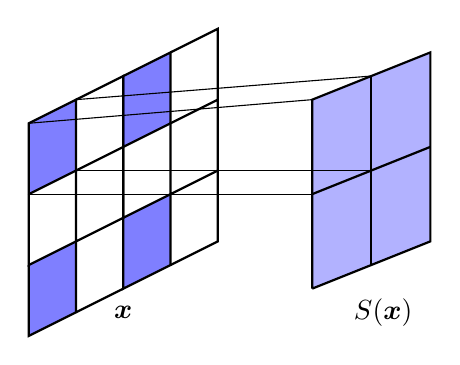
\begin{tikzpicture}[scale=0.6]
%\draw[opacity=0.5] (-4,-4) grid (4,4);

%%% grosse image

    % BLOCK (1,1)
% pixels bleu
\draw[thick, fill=blue, fill opacity=0.5] (-3,0) -- (-3,-1.5) -- (-4,-2)  -- (-4,-0.5);

% pixels blancs
\draw[thick, xshift=1cm, yshift=0.5cm] (-4,-2) -- (-3,-1.5);


    % BLOCK (2,1)
% pixels bleu
\draw[thick, fill=blue, fill opacity=0.5, xshift=2cm, yshift=1cm] (-3,0) -- (-3,-1.5) -- (-4,-2)  -- (-4,-0.5);

% pixels blancs
\draw[thick, xshift=3cm, yshift=1.5cm] (-3,0) -- (-3,-1.5) -- (-4,-2);

    % BLOCK (1,2)
% pixels bleu
\draw[thick, fill=blue, fill opacity=0.5, yshift=3cm] (-4,-2) -- (-4,-0.5) -- (-3,0) -- (-3,-1.5) -- (-4,-2);

% pixels blancs
\draw[thick, yshift=1.5cm] (-4,-0.5) -- (-4,-2) -- (-3,-1.5);
\draw[thick, xshift=1cm, yshift=3.5cm] (-4,-0.5) -- (-3,0) -- (-3,-1.5);

%pixels rouge
\draw[thick, xshift=1cm, yshift=2cm] (-4,-2) -- (-4,-0.5) -- (-3,0) -- (-3,-1.5) -- (-4,-2);

    % BLOCK (2,2)
% pixels bleu
\draw[thick, fill=blue, fill opacity=0.5, xshift=2cm, yshift=4cm] (-4,-2) -- (-4,-0.5) -- (-3,0) -- (-3,-1.5) -- (-4,-2);

% pixels blancs
\draw[thick, xshift=2cm, yshift=2.5cm] (-4,-0.5) -- (-4,-2) -- (-3,-1.5);
\draw[thick, xshift=3cm, yshift=4.5cm] (-4,-0.5) -- (-3,0) -- (-3,-1.5);

%pixels rouge
\draw[thick, xshift=3cm, yshift=3cm] (-4,-2) -- (-4,-0.5) -- (-3,0) -- (-3,-1.5) -- (-4,-2);

%%% petite image

\draw[thick, fill=blue, fill opacity=0.3, xshift=1cm] (1,-1) -- (1,3) -- (3.5,4) -- (3.5,0) -- (1,-1);
\draw[thick, xshift=2.25cm, yshift=0.5cm] (1,-1) -- (1,3);
\draw[thick, xshift=1cm, yshift=-2cm] (1,3) -- (3.5,4);

%%% lien

\draw (-4,1) -- (2,1);
\draw (-4,2.5) -- (2,3);
\draw (-3,1.5) -- (3.25,1.5);
\draw (-3,3) -- (3.25,3.5);

%%% Nom

\draw  (-2,-1.5) -- (-2,-1.5) node{$\bf{x}$};
\draw  (3.5,-1.5) -- (3.5,-1.5) node{$S(\bf{x})$};
\end{tikzpicture}}
\end{floatrow}
\end{figure}

\begin{figure}[h]\centering
    \setlength{\tabcolsep}{5pt}
\begin{tabular}{c c c c c}

\ Sans  &  $\sigma=0.5$  &  $\sigma=0.6$  &  $a=0.6$  &  $a=0.4$

\\

\rotatebox[origin=lt]{90}{{\color{white}bb}filtre}

\includegraphics[width=0.14\textwidth]{resultats/compare_filter/seed21-f-filtre=s.png}
&
\includegraphics[width=0.14\textwidth]{resultats/compare_filter/seed21-f-filtre=g_param=0.5.png}
&
\includegraphics[width=0.14\textwidth]{resultats/compare_filter/seed21-f-filtre=g_param=0.6.png}
&
\includegraphics[width=0.14\textwidth]{resultats/compare_filter/seed21-f-filtre=p_param=0.6.png}
&
\includegraphics[width=0.14\textwidth]{resultats/compare_filter/seed21-f-filtre=p_param=0.4.png}

\\

\rotatebox[origin=lb]{90}{{\color{white}b}image $\bf{x}$}

\includegraphics[width=0.14\textwidth]{resultats/compare_filter/seed21-x.png}
&
\includegraphics[width=0.14\textwidth]{resultats/compare_filter/seed21-x.png}
&
\includegraphics[width=0.14\textwidth]{resultats/compare_filter/seed21-x.png}
&
\includegraphics[width=0.14\textwidth]{resultats/compare_filter/seed21-x.png}
&
\includegraphics[width=0.14\textwidth]{resultats/compare_filter/seed21-x.png}

\\

\rotatebox[origin=lb]{90}{{\color{white}l}mesure $A\bf{x}$}

\includegraphics[width=0.14\textwidth]{resultats/compare_filter/seed21-Ax-filtre=s.png}
&
\includegraphics[width=0.14\textwidth]{resultats/compare_filter/seed21-Ax-filtre=g_param=0.5.png}
&
\includegraphics[width=0.14\textwidth]{resultats/compare_filter/seed21-Ax-filtre=g_param=0.6.png}
&
\includegraphics[width=0.14\textwidth]{resultats/compare_filter/seed21-Ax-filtre=p_param=0.6.png}
&
\includegraphics[width=0.14\textwidth]{resultats/compare_filter/seed21-Ax-filtre=p_param=0.6.png}
\end{tabular}
    \caption{Quelques exemples d'application de $A$ à un même image en fonction des filtres. }
\end{figure}

\begin{enonce}[Problématique]
On considère $\bf{x_0}\in\R^{n\times m}$ une image que l'on cherche à reconstruire et $\ \bf{y_0}:=A(\bf{x_0})\ $ sa version sous-échantillonnée. Une bonne reconstruction de $\bf{x_0}$ étant un minimiseur :
\begin{equation}\label{eq:probleme}
\bf{x^*}\in \argmin{\bf{x}\in\R^{n\times m}}\ F(\bf{x})\end{equation}\end{enonce}

Si pour le bien de l'étude $\bf{x_0}$ sera connu, il va de soit que le problème nécessite pas de le connaître \apriori.
\\
Aussi, la linéarité de $A$ assure la convexité de $F$ mais, bien évidemment, son caractère hautement non injectif (surtout pour $pq\lll nm$) fait qu'il existe tout un sous-espace affine de minimum globaux. D'où l'intérêt des deux méthodes étudiées pour ``choisir'' ce minimum.
\\

\begin{wrapfigure}{r}{0.4\textwidth}% vire le [16]
    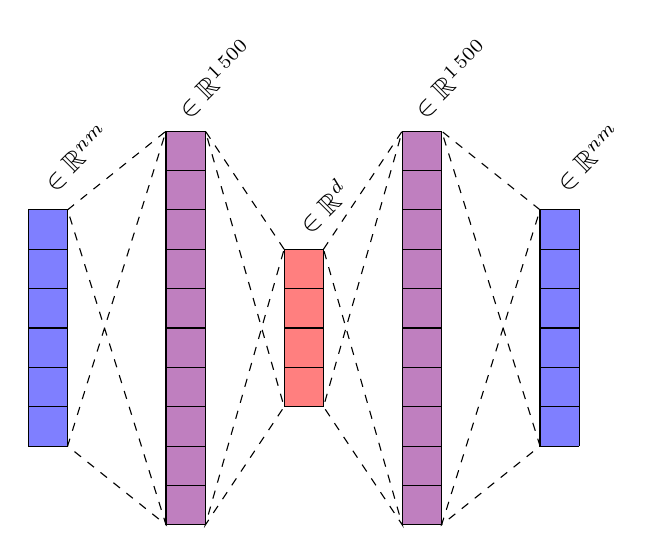
\begin{tikzpicture}[scale=0.5]
%\draw[thin, opacity=0.5] (-7.5,-6.5) grid (7.5,6.5);

%%% vecteurs

% input
\draw[fill=blue, fill opacity=0.5] (-7,-3) -- (-7,3) -- (-6,3)  -- (-6,-3) -- (-7,-3);
\draw (-7, 2) -- (-6, 2);
\draw (-7, 1) -- (-6, 1);
\draw (-7, 0) -- (-6, 0);
\draw (-7, -1) -- (-6, -1);
\draw (-7, -2) -- (-6, -2);

% hidden 1
\draw[fill=violet, fill opacity=0.5] (-3.5,-5) -- (-2.5,-5) -- (-2.5,5)  -- (-3.5,5) -- (-3.5,-5);
\draw (-3.5, 4) -- (-2.5, 4);
\draw (-3.5, 3) -- (-2.5, 3);
\draw (-3.5, 2) -- (-2.5, 2);
\draw (-3.5, 1) -- (-2.5, 1);
\draw (-3.5, 0) -- (-2.5, 0);
\draw (-3.5, -1) -- (-2.5, -1);
\draw (-3.5, -2) -- (-2.5, -2);
\draw (-3.5, -3) -- (-2.5, -3);
\draw (-3.5, -4) -- (-2.5, -4);

% latent
\draw[fill=red, fill opacity=0.5] (-0.5,-2) -- (0.5,-2) -- (0.5,2)  -- (-0.5,2) -- (-0.5,-2);
\draw (-0.5, 1) -- (0.5, 1);
\draw (-0.5, 0) -- (0.5, 0);
\draw (-0.5, -1) -- (0.5, -1);

% hidden 2
\draw[fill=violet, fill opacity=0.5] (3.5,-5) -- (2.5,-5) -- (2.5,5)  -- (3.5,5) -- (3.5,-5);
\draw (3.5, 4) -- (2.5, 4);
\draw (3.5, 3) -- (2.5, 3);
\draw (3.5, 2) -- (2.5, 2);
\draw (3.5, 1) -- (2.5, 1);
\draw (3.5, 0) -- (2.5, 0);
\draw (3.5, -1) -- (2.5, -1);
\draw (3.5, -2) -- (2.5, -2);
\draw (3.5, -3) -- (2.5, -3);
\draw (3.5, -4) -- (2.5, -4);

% output
\draw[fill=blue, fill opacity=0.5] (7,-3) -- (7,3) -- (6,3)  -- (6,-3) -- (7,-3);
\draw (7, 2) -- (6, 2);
\draw (7, 1) -- (6, 1);
\draw (7, 0) -- (6, 0);
\draw (7, -1) -- (6, -1);
\draw (7, -2) -- (6, -2);

%%% liens

\draw[dashed, thin] (-6,3) -- (-3.5,5) -- (-6,-3) -- (-3.5,-5) -- (-6,3);
\draw[dashed, thin] (-0.5,2) -- (-2.5,5) -- (-0.5,-2) -- (-2.5,-5) -- (-0.5,2);
\draw[dashed, thin] (0.5,2) -- (2.5,5) -- (0.5,-2) -- (2.5,-5) -- (0.5,2);
\draw[dashed, thin] (6,3) -- (3.5,5) -- (6,-3) -- (3.5,-5) -- (6,3);

%%% tailles

\draw (-5.75,4.25) -- (-5.75,4.25) node[]{\rotatebox[origin=lt]{45}{$\in\R^{nm}$}};
\draw (-2.25,6.25) -- (-2.25,6.25) node[]{\rotatebox[origin=lt]{45}{$\in\R^{1\,500}$}};
\draw (0.5,3) -- (0.5,3) node[]{\rotatebox[origin=lt]{45}{$\in\R^d$}};
\draw (3.75,6.25) -- (3.75,6.25) node[]{\rotatebox[origin=lt]{45}{$\in\R^{1\,500}$}};
\draw (7.25,4.25) -- (7.25,4.25) node[]{\rotatebox[origin=lt]{45}{$\in\R^{nm}$}};
\end{tikzpicture}
    \caption{Schéma des auto-encodeurs  $f$ avec $d=100,\ 200,\ 400,\ 800$}
    \label{fig:AEschem}
\end{wrapfigure}

Les auto-encodeurs utilisés pour paramétrer l'espace des images sont des réseaux MLP que l'on notera indifféremment $f$ et dont $f_E$ et $f_D$ sont les parties encodage et décodage :
\[f = f_E\circ f_D\]
Conformément à la figure \textit{\ref{fig:AEschem}}, ils se composent tous d'une couche cachées de taille $1\,500$ pour les parties encodeurs et décodeurs et la seule choses qui les différencies est la taille de leur espace latent qui variant entre $100$ et $800$. Leur entraînement s'est fait sur le jeu donnés MNIST et c'est donc uniquement sur ces images que seront présenté les résultats. Plus de détail sur les performances des auto-encodeurs en annexe \ref{anx:AE}. 
\\ 

TRANSITION ?
\\




\subsection{Cadre théorique de l'article}\label{sec:article1/2}

Comme expliqué plus tôt, tout l'objet de l'article \cite{traonmilin_basins_2022} est d'étudier dans quelle mesure il est possible de faire une descente de gradient sur une paramétrisation (non-convexe) d'un modèle plutôt que sur le modèle lui-même. 
\\
Pour cela, on note $\Sigma\subset\R^{n\times m}$ le modèle de basse-dimension et $\phi: \R^d\lr\R^{n\times m}$ une paramétrisation de ce dernier avec :
\begin{align*}\Sigma&\subset\phi\big(\R^d\big)  &  \Theta&:=\phi^{-1}(\Sigma)\end{align*}
\\
La paramétrisation $\phi$, doit vérifier certaines hypothèses de régularité pour pouvoir appliquer les résultats de l'article. Dans notre cas, $\ \phi=f_D\ $ dont les fonctions d'activations sont toutes des sigmoïdes. Elle est donc $C^{\infty}$ et pour cette raison on ne s'attardera pas outre mesure sur les questions de régularités de $\phi$.
\\

\textit{\`A noter qu'on ne suppose ni que $\ \phi(\R^d)=\Sigma\ $ ni que  $\ \Theta=\R^d$ et ce ne sera pas le cas pour nous. Aussi, le formalisme proposé par Traonmilin \etal est légèrement différent de celui donné en section précédente. Il y est considéré un espace de mesure $\mathcal{D}$ et les signaux (dans notre cas les images) sont pris dans $\mathcal{D}^*$, de sorte que la mesure par $\alpha\in\mathcal{D}$ de $x\in\mathcal{D}^*$ soit représenté par le crochet de dualité $\langle \alpha,x\rangle$. Cela à son intérêt surtout en dimension infinie, mais autrement, cette écriture est tout à fait équivalente à celle donnée en section \ref{sec:forma2pb}}
\\

\begin{wrapfigure}{r}{0.43\textwidth}
    \fbox{\begin{minipage}{15em}
\vspace{0.3cm}
\begin{algorithmic}[0]
    \State $\theta_0$ : initialisation
    \State $x$ : image à reconstruire
    \State $\tau$ : pas de descente
    \State $N$ : nombre d'itération
    \State $\hat{x}\ \longleftarrow\ f(x)$
    \State
    \For{$n\in \llbracket1,N-1\rrbracket$}
        \State $\theta_{n+1}\ \longleftarrow\ \theta_n\ - \tau \nabla g(\theta_un)$
        \State $x_{n+1}\ \longleftarrow\ f_D(\theta_{n+1})$
        \EndFor
    \State
    \Return $(x_n)_{0\leq n\leq N}$
\end{algorithmic}
\vspace{0.2cm}
\end{minipage}}
    \caption{Algorithme de descente depuis l'espace des paramètres}
    \label{fig:pcode LGD}
\end{wrapfigure}

Le problème est donc de trouver les paramètres $\theta^*$ minimisant $\ g:=A\phi\ $ sur $\Theta$, ou dans notre cas :
\[\theta^*\in\argmin{\theta\in\Theta}\ \frac{1}{2}{\big\|Af_D(\theta)-\bf{y_0}\big\|_2}^2\]
\\
Minimum que l'on cherche à les obtenir par descente de gradient. On considérera donc dans toute la suite, $(\theta_n)$ la descente de gradient à pas fixe, $\forall\theta_0\in\R^d$ :
\[\forall n\in\N^*,\qquad \theta_{n+1} = \theta_n - \tau\nabla g(\theta_n)\]
Sachant que $\phi$ est n'est pas convexe, on introduit la définition suivante :
\\ \\
\begin{definition} 
Une partie $\Lambda\subset\Theta$ de $\R^d$ sera un \emph{bassin d'attraction} de minimum globale $\theta^*\in\Lambda$ si en tout point $\theta_0\in\Lambda$, alors existe un pas de descente $\tau_0$ tel que :
\[\forall \tau\in]0,\tau_0],\qquad \lim_{n\lr+\infty}g\big(\theta_n\big)=g(\theta^*)\]
\end{definition}

Avec cette définition, $(\theta_n)$ peut tout à fait converger vers un autre minimum que $\theta^*$. Pour en tenir compte en même temps que la potentielle non-injectivité de $\phi$, ils introduisent les définitions suivantes :
\\
\begin{definition}\label{def:boule}
On note $d(\theta,\theta^*)$ la distance de $\theta$ au plus proche paramètre de même image de $\theta^*$ et $p(\theta,\theta^*)$ la projection (potentiellement multivaluée) de $\theta$ sur ce même paramètre, e.i. sur $\phi^{-1}\circ\phi(\{\theta^*\})$ :
 $\forall\theta\in\R^d$ :
\begin{align*}d(\theta,\theta^*) &:=\min_{\substack{\Tilde{\theta}\in\Theta\\ \phi(\Tilde{\theta})=\phi(\theta^*)}}\ \big\|\Tilde{\theta}-\theta\big\|_2  &  p(\theta,\theta^*)&:=\argmin{\substack{\Tilde{\theta}\in\Theta\\ \phi(\Tilde{\theta})=\phi(\theta^*)}}\ \big\|\Tilde{\theta}-\theta\big\|_2\subset\R^d\end{align*}
Avec, sont définis les bassins $\Lambda_\beta(\theta^*)$ de la forme :
\[\forall \beta\in\R^{+_*},\qquad \Lambda_\beta(\theta^*):=\big\{\theta\in\R^d\ |\ d(\theta, \theta^*)<\beta\big\}\]
\end{definition}

Contrairement aux exemples traités dans l'article, la paramétrisation par l'espace latent ne donne pas de formule vraiment exploitable pour $\phi=f_D$. En revanche, $f_D$ faisant parti d'un auto-encodeur, on peut supposer que $f_E$ est la réciproque de $f_D$ au moins sur $\Theta$ :
\begin{align*} {{f_{D}}_{\displaystyle |_{\Theta}}}^{-1}&={f_{E}}_{\displaystyle |_{\Sigma}}  & &\text{avec} & \Theta&=f_E(\Sigma)
\end{align*}
\\
En particulier, cela permet d'avoir l'injectivité de $f_D$ sur $\Theta$. Ce dont il découle que $d(\theta,\theta^*)=\|\theta-\theta^*\|_2$ est une distance (ce qui n'est pas le cas en générale), que $\Lambda_\beta(\theta^*)$ une boule ouverte et que $\ p(\theta,\theta^*)=\theta^*$.
\\

Enfin, dans toute la suite $\Sigma$ sera supposé être un cône, c'est-à-dire que pour tout $\lambda>0$, $\lambda\Sigma=\Sigma\ $ et sont introduites les deux ensembles suivants :
\\

\begin{definition} On appelle \emph{ensemble des sécantes de $\Sigma$} l'ensemble :
\[\mathcal{S}(\Sigma) := \Sigma-\Sigma = \big\{x-y\in\R^{n\times m}\ |\ x,y\in\Sigma\big\}\]
\\
En notant $\partial_u\phi(\theta)$ la dérivée directionnelle de $\phi$ en $\theta$ et dans la direction $u$, on définie l'\emph{ensemble généralisé des sécantes de $\Sigma$}, l'ensemble noté :
\[\overline{\mathcal{S}(\Sigma)}:=\mathcal{S}(\Sigma)\cup\Big\{\partial_u\phi(\theta)\ |\ \forall (\theta,u)\in\Theta\times\R^d\Big\}\]{\color{white}l}

\emph{Pour nous, $\phi=f_D\ $ est $C^\infty$, donc la dérivée directionnelle $\partial_u\phi(u)$ est équivalente à la différentiel de $\phi$ au point $\theta$ valué en $u$, $D_\theta\phi(u)$.}
\end{definition}

L'auto-encodeur $f$ n'a été entraîné que sur des images dont les pixels prennent valeur dans $[0,1]$ et il n'est capable de reconstruire que ce type d'image. Et ceux, pour la simple et bonne raison que ses fonctions d'activations sont des sigmoïdes y compris les celles sorties. Il est donc strictement impossible qu'une image $f_D(\theta)$ prenne des valeurs au delà de 1, ce qui va à l'encontre de l'hypothèse que $\Sigma$ soit un cône.
\\
Si ce choix de fonction d'activation à été fait c'était à l'origine pour reprendre les codes de l'article \cite{peng_solving_2019} sur la descente projeté (voir section \ref{sec:comparPGD}), mais en toute vraisemblance utiliser des fonctions ReLu ou autre ne devrait pas trop changer les résultats obtenus. 
La perte de régularité entraîné ne devrait pas non plus être un problème en pratique et pourrait rendre l'hypothèse un peu plus raisonnable. 
\\




\subsection{Les résultats de Traonmilin {\itshape et al.}}\label{sec:article2/2}

Le théorème de Traonmilin \etal, dans le cas sans bruit, s'énonce ainsi :
\\
\begin{theoreme}[sans bruit]\label{theo:maintheo} Soit $\theta^*\in\Theta$ un minimiseur globale de $g$. Si on a les hypothèses suivantes :
\begin{itemize}
    \item l'opérateur de mesure $A$ est continue et vérifie la \emph{propriété d'isométrie restreinte} (RIP) de constante $\gamma\in]0,1]$ :
\begin{equation}\label{eq:RIP}
\forall v\in\overline{\mathcal{S}(\Sigma)},\qquad (1-\gamma)\|v\|^2\leq \|Av\|^2\leq (1+\gamma)\|v\|^2
\end{equation}

    \item Si $\Lambda_{2\beta}(\theta^*)$, tel que définie en \ref{def:boule}, est inclus dans $\Theta$, ou autrement dit :
\begin{equation}\label{eq:LambinTheta}
\phi\big(\Lambda_{2\beta}\big)\subset\Sigma
\end{equation}

    \item Si la \emph{technical assumption} \ref{hyp:technical} (donné plus bas) est vérifier sur $\Lambda_{2\beta}$ avec la constante $C>0$ et qu'il existe $\Tilde{\theta}\in p(\theta,\theta^*)$ tel qu'on ait l'inégalité :
\begin{equation}\label{eq:majo3}
\forall z\in[\theta,\Tilde{\theta}],\qquad \frac{(1-\gamma){\big\|\partial_{\Tilde{\theta}-\theta}\phi(z)\big\|_2}^2}{\sqrt{1+\gamma}\big\|A\partial^2_{\Tilde{\theta}-\theta}\phi(z)\big\|_2}\geq C\beta
\end{equation}
\end{itemize}

Si $A$ et $\phi$ vérifie de plus la \emph{framework assumption} \ref{hyp:framework}, alors l'ensemble $\Lambda_\beta(\theta^*)$ est un bassin d'attraction.  
\end{theoreme}

\begin{corollaire}
En particulier, s'il existe une constante $\beta_1>0$ vérifiant la \emph{technical assumption} \ref{hyp:technical} et telle que $p(\,\cdot\,, \theta^*)$ soit mono-valuée sur $\Lambda_{\beta_1}(\theta^*)$ :
\[\forall \theta\in\Lambda_{\beta_1}(\theta^*),\qquad p(\theta,\theta^*)=\big\{\Tilde{\theta}\big\}\]
\\
Alors $\Lambda_{\min(\beta_1,\beta_2)}(\theta^*)$ est un bassin d'attraction, où $\beta_2$ est donné par la formule :
\[\beta_2:=\frac{1-\gamma}{C\sqrt{1+\gamma}}\inf_{\theta\in\Lambda_{\beta_1}(\theta^*)}\inf_{z\in[\theta,\Tilde{\theta}]}\frac{{\big\|\partial_{\Tilde{\theta}-\theta}\phi(z)\big\|_2}^2}{\big\|A\partial^2_{\Tilde{\theta}-\theta}\phi(z)\big\|_2}\]
\end{corollaire}

Ce théorème (et son corollaire) donne une estimation de la marge que l'on a autour de $\theta^*$ pour initialiser la descente de gradient depuis l'espace des paramètres de sorte à s'assurer sa convergence. En particulier, l'inégalité \ref{eq:majo3} donne, sachant $\gamma$ et $C$, à quel point le ``rayon'' du bassin $\beta$ peut être grand.
Estimation qui est donc valable sachant les deux hypothèses supplémentaires :
\\
\begin{assump}[Technical assumption]\label{hyp:technical}
La \emph{technical assumption} est vérifier sur $\Lambda_{2\beta}(\theta^*)$ avec la constante $C>0$ si elle donne un contrôle de $d$ sur $\|\cdot\|_2$ :
\[\forall\theta\in\Lambda_{2\beta}(\theta^*),\qquad \big\|\theta-\theta^*\big\|_2\leq C d\big(\theta, \theta^*\big)\]
et si les deux premières dérivées (directionnelles) de $A\phi$ sont uniformément bornées respectivement sur $\phi^{-1}\circ\phi(\{\theta^*\})$ et $\Lambda_{2\beta}$ :
\begin{align*}\sup_{\theta\in\phi^{-1}\circ\phi(\{\theta^*\})}\sup_{\|u\|_2=1}\big\|A\partial_u\phi(\theta)\big\|_2&<+\infty  &  \sup_{\theta\in\Lambda_{2\beta}(\theta^*)}\sup_{\|u\|_2,\|v\|_2=1}\big\|A\partial_u\partial_v\phi(\theta)\big\|_2&<+\infty 
\end{align*}
\end{assump}

Comme dit plus haut, supposer $\phi=f_D$ inversible sur $\Theta$ impose $\ d\big(\theta, \theta^*\big)=\big\|\theta-\theta^*\big\|_2$. Ainsi la première inégalité est vérifié pour tout $C\geq1$ et les majorations uniformes ne sont pas un problème non plus puisque que $f_D$ est $C^\infty$. Sachant que c'est l'inégalité \ref{eq:majo3} qui nous intéresse, on va plutôt avoir tendance à prendre $C=1$.
\\

\begin{assump}[Framework assumption]\label{hyp:framework}
La paramétrisation $\phi$ doit être deux fois (Gateaux) différentiable et il faut que pour toute suite $|h_n|\xrightarrow[n\lr+\infty]{} 0$, $\left\|\frac{\phi(\theta +|h_n|v)-\phi(\theta)}{|h_n|}\right\|_2$ converge indépendant de $(|h_n|)$ et ceux, pour tout $(\theta,v)$ tel que $\partial_v\phi(\theta)\in\overline{\mathcal{S}(\Sigma)}$.
\end{assump}

Dans l'article \cite{traonmilin_basins_2022}, la mesure de proximité des images est fait à travers une norme $\|\cdot\|_\mathcal{H}$ associé un espace hilbertien $\mathcal{H}$ contenant $\Sigma$. Cette hypothèse permet alors de s'assurer que cette norme s'étende à $\overline{\mathcal{S}(\Sigma})$. Mais encore, une fois, pour nous $\mathcal{H}=\R^{n\times m}$ et il n'y a pas de risque à ce sujet. Aussi, le fait que $\phi=f_E$ soit différentiable rend immédiat la convergence de la suite $\left\|\frac{\phi(\theta +|h_n|v)-\phi(\theta)}{|h_n|}\right\|_2$ indépendamment de $\big(|h_n|\big)_n$.
\\ \\

Revenons maintenant sur les autres hypothèses du théorèmes. 
\\
D'abord, dans la RIP (\ref{eq:RIP}), c'est surtout l'inégalité de gauche qui est important puisqu'elle garantie que $A$ soit inversible sur $\overline{\mathcal{S}(\Sigma)}$.
\\
Comme $\Sigma$ n'est pas proprement définie, le mieux qu'on puisse faire c'est de vérifier si c'est au moins le cas pour tout les $\bf{x}-\bf{y}$ avec $\bf{x}$, $\bf{y}$ du jeu de données (MNIST donc). Pour se faire, on les équivalences :
\begin{align*}(1-\gamma)\|v\|^2\leq \|Av\|^2\leq (1+\gamma)\|v\|^2\ &\Llr\ \frac{\|Av\|^2}{\|v\|^2}-1\leq \gamma\\
    &\Llr\ \left|\frac{\|Av\|^2}{\|v\|^2}-1\right|\leq \gamma\end{align*}
En calculant le rapport $\left|\frac{\|Av\|^2}{\|v\|^2}-1\right|$, on peut donc estimer une borne pour $\gamma$. Seulement, avec les moyens disponibles et notre code, passer en revue les $60\,000\times(60\,000+1)$ couples d'images du set de test demanderait quelque $11$h de calcul. On se contentera donc, faute de mieux, de faire les calculs sur $\Sigma$, ce qui nous donnes les histogrammes \textit{\ref{fig:RIP-s}} et \textit{\ref{fig:RIP-g}} :
\\

\begin{figure}[h]
\begin{floatrow}
\ffigbox{\caption{Histogramme des valeurs de $\big|{\|Av\|_2}^2/{\|v\|_2}^2-1\big|$ sans filtre passe-bas sur le set de test}\label{fig:RIP-s}}
{% This file was created with tikzplotlib v0.10.1.
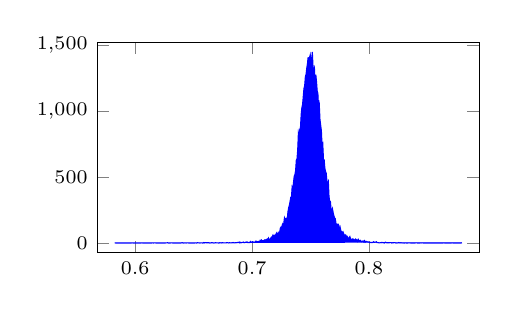
\begin{tikzpicture}

\definecolor{darkgray176}{RGB}{176,176,176}
\definecolor{steelblue31119180}{RGB}{31,119,180}

\begin{axis}[standard]
\addplot [blue, fill=blue]
table {%
0.582521796226501 1
0.583117008209229 0
0.596806526184082 0
0.597401738166809 1
0.597996950149536 0
0.605139255523682 0
0.605734586715698 1
0.606329679489136 0
0.614067316055298 0
0.614662408828735 1
0.615257740020752 0
0.615852832794189 0
0.616448044776917 1
0.617043256759644 1
0.617638468742371 0
0.62597119808197 0
0.626566410064697 1
0.627161622047424 1
0.627756834030151 2
0.628351926803589 0
0.63013768196106 0
0.630732774734497 1
0.631327986717224 1
0.631923198699951 0
0.639065504074097 0
0.640255928039551 2
0.640851140022278 0
0.642041563987732 0
0.642636775970459 1
0.643231868743896 0
0.643827199935913 0
0.644422292709351 1
0.645017623901367 1
0.645612716674805 0
0.650969505310059 0
0.651564717292786 1
0.652159929275513 0
0.65275502204895 0
0.653350353240967 2
0.653945446014404 1
0.654540777206421 1
0.655135869979858 0
0.655731081962585 0
0.656326293945312 1
0.65692150592804 1
0.657516717910767 0
0.658111810684204 0
0.658707141876221 3
0.659302234649658 0
0.659897565841675 3
0.661087870597839 1
0.661683082580566 2
0.662278294563293 1
0.662873506546021 2
0.663468599319458 0
0.664063930511475 1
0.664659023284912 0
0.665254235267639 2
0.665849447250366 2
0.66703987121582 0
0.667634963989258 0
0.668825387954712 2
0.669420719146729 1
0.670611023902893 1
0.67120623588562 0
0.671801447868347 0
0.672396659851074 2
0.673587083816528 0
0.674182176589966 2
0.674777388572693 2
0.67537260055542 1
0.677753448486328 1
0.678943872451782 3
0.67953896522522 1
0.680134177207947 0
0.680729389190674 2
0.681324601173401 1
0.682514905929565 1
0.683110237121582 3
0.68370532989502 1
0.684300661087036 3
0.684895753860474 1
0.685490965843201 1
0.686086177825928 3
0.686681389808655 2
0.688467025756836 5
0.689062118530273 1
0.689657330513 7
0.690252542495728 2
0.690847754478455 2
0.691442966461182 4
0.692038059234619 4
0.692633390426636 7
0.693228483200073 2
0.69382381439209 3
0.694418907165527 6
0.695014119148254 5
0.695609331130981 8
0.696204543113708 3
0.696799755096436 3
0.697394847869873 4
0.69799017906189 3
0.698585271835327 11
0.699180603027344 5
0.699775695800781 7
0.700370907783508 10
0.701561331748962 6
0.702156543731689 7
0.702751636505127 6
0.703346967697144 14
0.703942060470581 7
0.705132484436035 11
0.705727696418762 11
0.706322908401489 7
0.706918001174927 20
0.707513332366943 14
0.708108425140381 22
0.708703756332397 16
0.709298849105835 17
0.709894061088562 15
0.710489273071289 22
0.711084485054016 16
0.711679697036743 24
0.712274789810181 25
0.712870121002197 30
0.713465213775635 19
0.714060544967651 37
0.714655637741089 27
0.715250849723816 22
0.715846061706543 34
0.71644127368927 43
0.717036485671997 37
0.717631578445435 54
0.718226909637451 38
0.718822002410889 59
0.719417214393616 50
0.720012426376343 57
0.72060763835907 70
0.721202850341797 78
0.721797943115234 59
0.722393274307251 66
0.722988367080688 82
0.723583698272705 79
0.724178791046143 111
0.72477400302887 121
0.725369215011597 119
0.725964426994324 139
0.726559638977051 117
0.727154731750488 150
0.727750062942505 191
0.728345155715942 178
0.728940367698669 186
0.729535579681396 188
0.730130791664124 181
0.730726003646851 237
0.731321215629578 267
0.731916427612305 285
0.732511520385742 313
0.733106851577759 346
0.733701944351196 346
0.734297156333923 425
0.73489236831665 414
0.736082792282104 506
0.736677885055542 518
0.737273216247559 549
0.737868309020996 628
0.738463640213013 638
0.73905873298645 706
0.739653944969177 834
0.740249156951904 809
0.740844368934631 860
0.741439580917358 876
0.742034673690796 973
0.742630004882812 1026
0.74322509765625 1049
0.744415521621704 1171
0.745010733604431 1191
0.745605945587158 1260
0.746201038360596 1277
0.746796369552612 1324
0.74739146232605 1358
0.747986793518066 1408
0.748581886291504 1335
0.749177098274231 1405
0.749772310256958 1425
0.750367522239685 1371
0.750962734222412 1388
0.75155782699585 1447
0.752153158187866 1335
0.752748250961304 1311
0.75334358215332 1327
0.753938674926758 1198
0.754533886909485 1276
0.755129098892212 1223
0.755724310874939 1151
0.756319522857666 1134
0.756914615631104 1017
0.75750994682312 1047
0.758105039596558 934
0.759295463562012 850
0.759890675544739 735
0.760485887527466 751
0.761080980300903 635
0.76167631149292 631
0.762271404266357 566
0.762866735458374 542
0.763461828231812 527
0.764057040214539 466
0.764652252197266 455
0.765247464179993 467
0.76584267616272 350
0.766437768936157 312
0.767033100128174 314
0.767628192901611 252
0.768223404884338 237
0.768818616867065 258
0.769413828849792 227
0.77000904083252 206
0.770604252815247 190
0.771199464797974 184
0.772389888763428 112
0.772984981536865 142
0.773580193519592 143
0.774175405502319 133
0.774770617485046 97
0.775365829467773 118
0.775960922241211 94
0.776556253433228 84
0.777151346206665 81
0.777746677398682 86
0.778341770172119 70
0.778936982154846 61
0.779532194137573 54
0.7801274061203 60
0.780722618103027 50
0.781317710876465 51
0.781913042068481 39
0.782508134841919 30
0.783103346824646 40
0.783698558807373 48
0.7842937707901 28
0.784888982772827 28
0.785484075546265 29
0.786079406738281 31
0.786674499511719 29
0.787269830703735 16
0.7884601354599 30
0.789650559425354 22
0.790245771408081 13
0.790840864181519 27
0.791436195373535 18
0.792031288146973 18
0.792626619338989 20
0.793221712112427 13
0.793816924095154 10
0.794412136077881 14
0.795007348060608 15
0.795602560043335 8
0.796197652816772 17
0.796792984008789 6
0.797388076782227 11
0.797983288764954 11
0.798578500747681 9
0.799173712730408 8
0.799768924713135 8
0.800364017486572 3
0.800959348678589 5
0.801554441452026 3
0.802149772644043 4
0.80274486541748 3
0.803340077400208 5
0.803935289382935 9
0.804530501365662 5
0.805720806121826 7
0.806316137313843 9
0.80691123008728 3
0.807506561279297 3
0.808696866035461 1
0.809292078018188 1
0.809887290000916 3
0.810482501983643 2
0.81107759475708 5
0.812268018722534 1
0.812863230705261 3
0.813458442687988 0
0.814053654670715 6
0.814648866653442 4
0.81524395942688 1
0.815839290618896 2
0.816434383392334 1
0.817029714584351 2
0.817624807357788 2
0.818220019340515 3
0.818815231323242 3
0.819410443305969 0
0.820005655288696 2
0.820600748062134 0
0.82119607925415 3
0.821791172027588 3
0.822386384010315 2
0.822981595993042 0
0.823576807975769 0
0.824172019958496 1
0.824767231941223 0
0.82536244392395 3
0.825957536697388 2
0.826552867889404 0
0.827147960662842 2
0.828338384628296 0
0.828933596611023 1
0.82952880859375 0
0.830719232559204 0
0.831314325332642 1
0.831909656524658 0
0.833099961280823 0
0.83369517326355 1
0.834290385246277 0
0.834885597229004 1
0.835480690002441 0
0.839647054672241 0
0.840242385864258 1
0.840837478637695 1
0.841432809829712 0
0.843813538551331 0
0.844408750534058 1
0.845003843307495 0
0.845599174499512 1
0.846194267272949 0
0.863455057144165 0
0.864050269126892 1
0.864645481109619 0
0.870597362518311 0
0.871192693710327 1
0.871787786483765 0
0.87893009185791 0
0.879525423049927 2
};
\end{axis}

\end{tikzpicture}
}

\ffigbox{\caption{Histogramme des valeurs de $\big|{\|Av\|_2}^2/{\|v\|_2}^2-1\big|$ avec filtre gaussien ($\sigma=0,6$) sur le set de test}\label{fig:RIP-g}}
{% This file was created with tikzplotlib v0.10.1.
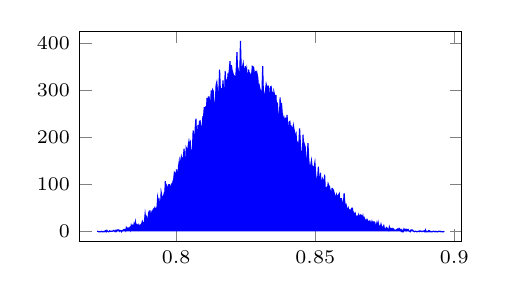
\begin{tikzpicture}

\definecolor{darkgray176}{RGB}{176,176,176}
\definecolor{steelblue31119180}{RGB}{31,119,180}

\begin{axis}[standard]
\addplot [blue, fill=blue]
table {%
0.771571159362793 1
0.771821260452271 1
0.772071480751038 0
0.772822022438049 0
0.773072242736816 1
0.773322343826294 0
0.773822784423828 0
0.774072885513306 1
0.774322986602783 0
0.77457332611084 2
0.774823427200317 0
0.775073528289795 3
0.775323867797852 1
0.775573968887329 0
0.775824069976807 0
0.776074409484863 2
0.776324510574341 1
0.777075052261353 1
0.777575373649597 3
0.777825593948364 1
0.778075695037842 0
0.778325915336609 3
0.778576135635376 1
0.778826236724854 4
0.779326677322388 4
0.779576778411865 1
0.779826998710632 3
0.780077219009399 3
0.780327320098877 0
0.780577540397644 2
0.781328082084656 5
0.781578302383423 5
0.7818284034729 2
0.782078623771667 9
0.782328844070435 6
0.782578945159912 8
0.782829165458679 8
0.783079385757446 7
0.783329486846924 9
0.783579707145691 4
0.783829927444458 14
0.784080028533936 10
0.784330248832703 13
0.78458046913147 7
0.784830570220947 16
0.785080790519714 10
0.785331010818481 21
0.785581111907959 12
0.785831332206726 15
0.786081552505493 13
0.786331653594971 15
0.786581873893738 7
0.786832094192505 14
0.787082195281982 14
0.78733241558075 15
0.787582635879517 17
0.787832736968994 22
0.788082838058472 18
0.788333177566528 17
0.788583278656006 21
0.788833379745483 38
0.78908371925354 26
0.789333820343018 31
0.789583921432495 24
0.789834260940552 24
0.790084362030029 40
0.790334463119507 44
0.790584802627563 44
0.790834903717041 31
0.791085004806519 36
0.791335225105286 44
0.791585445404053 44
0.79183554649353 48
0.792085766792297 46
0.792335987091064 51
0.792586088180542 47
0.793086528778076 51
0.793336629867554 73
0.793586850166321 64
0.793837070465088 68
0.794087171554565 54
0.794337391853333 52
0.7945876121521 84
0.794837713241577 76
0.795087933540344 72
0.795338153839111 72
0.795588254928589 79
0.795838475227356 71
0.796088695526123 107
0.796338796615601 88
0.796589016914368 96
0.796839237213135 89
0.797089338302612 94
0.797339558601379 100
0.797589778900146 100
0.797839879989624 84
0.798090100288391 96
0.798340320587158 100
0.798590421676636 94
0.798840641975403 107
0.79909086227417 110
0.799340963363647 126
0.799591183662415 124
0.799841403961182 107
0.800091505050659 132
0.800341725349426 121
0.800591945648193 122
0.800842046737671 138
0.801092267036438 149
0.801342487335205 129
0.801592588424683 150
0.80184280872345 159
0.802093029022217 151
0.802343130111694 156
0.802593231201172 159
0.802843570709229 176
0.803093671798706 144
0.803343772888184 140
0.80359411239624 178
0.803844213485718 174
0.804094314575195 169
0.804344654083252 183
0.804594755172729 192
0.804844856262207 182
0.805095195770264 188
0.805345296859741 162
0.805595397949219 172
0.805845618247986 174
0.806095838546753 215
0.80634593963623 197
0.806596159934998 189
0.806846380233765 220
0.807096481323242 240
0.807346701622009 199
0.807596921920776 198
0.807847023010254 226
0.808097243309021 199
0.808347463607788 234
0.808597564697266 235
0.8090980052948 213
0.809348106384277 222
0.809598326683044 244
0.809848546981812 244
0.810098648071289 264
0.810348868370056 232
0.810599088668823 266
0.810849189758301 256
0.811099410057068 284
0.811349630355835 261
0.811599731445312 286
0.81184995174408 286
0.812100172042847 255
0.812350273132324 267
0.812600493431091 300
0.812850713729858 267
0.813100814819336 301
0.813351035118103 298
0.81360125541687 265
0.813851356506348 259
0.814101576805115 278
0.814351797103882 311
0.814601898193359 317
0.814852118492126 298
0.815102338790894 291
0.815352439880371 298
0.815602660179138 344
0.815852880477905 305
0.816102981567383 304
0.81635308265686 298
0.816603422164917 300
0.816853523254395 321
0.817103624343872 282
0.817353963851929 271
0.817604064941406 341
0.817854166030884 310
0.81810450553894 323
0.818354606628418 303
0.818604707717896 333
0.818855047225952 331
0.81910514831543 343
0.819355249404907 362
0.819605588912964 330
0.819855690002441 353
0.820105791091919 342
0.820356011390686 338
0.820606231689453 331
0.820856332778931 331
0.821106553077698 319
0.821356773376465 323
0.821606874465942 345
0.821857094764709 381
0.822107315063477 328
0.822357416152954 341
0.822607636451721 331
0.822857856750488 331
0.823107957839966 405
0.823358178138733 352
0.8236083984375 337
0.823858499526978 349
0.824108719825745 357
0.824358940124512 342
0.824609041213989 284
0.824859261512756 351
0.825109481811523 333
0.825359582901001 344
0.825609803199768 324
0.825860023498535 327
0.826110124588013 344
0.82636034488678 290
0.826610565185547 334
0.826860666275024 331
0.827110886573792 331
0.827361106872559 351
0.827611207962036 350
0.827861428260803 348
0.82811164855957 336
0.828361749649048 305
0.828611969947815 341
0.828862190246582 307
0.82911229133606 334
0.829362511634827 326
0.829612731933594 302
0.829862833023071 310
0.830113053321838 303
0.830363273620605 298
0.830613374710083 278
0.830863475799561 299
0.831113815307617 351
0.831363916397095 290
0.831614017486572 276
0.831864356994629 293
0.832114458084106 300
0.832364559173584 313
0.832614898681641 307
0.832864999771118 291
0.833115100860596 310
0.833365440368652 286
0.83361554145813 284
0.833865642547607 307
0.834115862846375 308
0.834366083145142 297
0.834616184234619 295
0.834866404533386 274
0.835116624832153 297
0.835366725921631 290
0.835616946220398 258
0.835867166519165 290
0.836117267608643 259
0.83636748790741 274
0.836617708206177 254
0.836867809295654 241
0.837118029594421 240
0.837368249893188 285
0.837618350982666 237
0.837868571281433 273
0.8381187915802 252
0.838368892669678 246
0.838619112968445 224
0.838869333267212 239
0.839119434356689 232
0.839369654655457 242
0.839619874954224 211
0.839869976043701 248
0.840120196342468 220
0.840370416641235 187
0.840620517730713 233
0.84087073802948 234
0.841120958328247 218
0.841371059417725 223
0.841621279716492 219
0.841871500015259 217
0.842121601104736 226
0.842371821403503 217
0.842622041702271 210
0.842872142791748 199
0.843122363090515 206
0.843372583389282 185
0.84362268447876 188
0.843872904777527 173
0.844123125076294 186
0.844373226165771 219
0.844623446464539 191
0.844873666763306 171
0.845123767852783 169
0.845373868942261 160
0.845624208450317 206
0.845874309539795 159
0.846124410629272 185
0.846374750137329 180
0.846624851226807 159
0.846874952316284 149
0.847125291824341 154
0.847375392913818 188
0.847625494003296 157
0.847875833511353 139
0.84812593460083 136
0.848376035690308 141
0.848626255989075 151
0.848876476287842 139
0.849126577377319 138
0.849376797676086 127
0.849627017974854 138
0.849877119064331 147
0.850127339363098 125
0.850377559661865 110
0.850627660751343 110
0.85087788105011 114
0.851128101348877 138
0.851378202438354 91
0.851628422737122 113
0.851878643035889 125
0.852128744125366 100
0.8526291847229 112
0.852879285812378 106
0.853129506111145 101
0.853379726409912 121
0.85362982749939 88
0.853880047798157 92
0.854130268096924 94
0.854380369186401 90
0.854630589485168 102
0.854880809783936 98
0.855130910873413 96
0.85538113117218 72
0.855631351470947 83
0.855881452560425 68
0.856131672859192 93
0.856381893157959 77
0.856631994247437 86
0.856882214546204 80
0.857132434844971 72
0.857382535934448 74
0.857632756233215 79
0.857882976531982 73
0.85813307762146 76
0.858383297920227 78
0.858633518218994 81
0.858883619308472 63
0.859133839607239 70
0.859384059906006 70
0.859634160995483 65
0.859884262084961 53
0.860134601593018 58
0.860384702682495 82
0.860634803771973 62
0.860885143280029 48
0.861135244369507 56
0.861385345458984 50
0.861635684967041 46
0.861885786056519 50
0.862135887145996 41
0.862386226654053 45
0.86263632774353 40
0.862886428833008 47
0.863136649131775 50
0.863386869430542 50
0.86363697052002 36
0.863887190818787 40
0.864137411117554 36
0.864387512207031 39
0.864637732505798 33
0.864887952804565 26
0.865138053894043 32
0.86538827419281 29
0.865638494491577 36
0.865888595581055 31
0.866138815879822 34
0.866389036178589 36
0.866639137268066 34
0.866889357566833 27
0.867139577865601 33
0.867389678955078 20
0.867639899253845 29
0.867890119552612 25
0.86814022064209 25
0.868390440940857 19
0.868640661239624 26
0.868890762329102 23
0.869140982627869 21
0.869641304016113 23
0.86989152431488 18
0.870141744613647 16
0.870391845703125 22
0.870642066001892 16
0.870892286300659 21
0.871142387390137 21
0.871392607688904 20
0.871642827987671 13
0.871892929077148 11
0.872143149375916 18
0.872393369674683 9
0.87264347076416 19
0.872893691062927 11
0.873143911361694 12
0.873394012451172 10
0.873644113540649 16
0.873894453048706 10
0.874144554138184 9
0.874394655227661 10
0.874644994735718 13
0.874895095825195 6
0.875145196914673 4
0.875395536422729 7
0.875645637512207 9
0.876396179199219 3
0.876646280288696 10
0.876896619796753 4
0.87714672088623 7
0.877396821975708 6
0.877647042274475 7
0.877897262573242 4
0.87814736366272 6
0.878397583961487 4
0.878647804260254 3
0.878897905349731 3
0.879648447036743 6
0.87989866733551 4
0.880148887634277 7
0.880398988723755 5
0.880649209022522 5
0.880899429321289 1
0.881149530410767 4
0.881399750709534 0
0.881649971008301 0
0.881900072097778 6
0.882150292396545 4
0.882400512695312 5
0.88265061378479 2
0.882900834083557 5
0.883151054382324 4
0.883401155471802 5
0.883651375770569 2
0.884151697158813 0
0.884401917457581 4
0.884902238845825 4
0.885152459144592 2
0.885652780532837 0
0.885903000831604 1
0.886153221130371 1
0.886403322219849 0
0.886653542518616 0
0.886903762817383 1
0.88715386390686 1
0.887404084205627 0
0.887654304504395 2
0.887904405593872 1
0.88815450668335 1
0.888404846191406 0
0.888654947280884 1
0.888905048370361 1
0.889155387878418 2
0.889405488967896 0
0.889655590057373 4
0.88990592956543 0
0.890406131744385 0
0.890656471252441 2
0.890906572341919 0
0.891156673431396 2
0.891406893730164 0
0.892157435417175 0
0.892407655715942 1
0.89265775680542 1
0.892907977104187 0
0.893158197402954 0
0.893408298492432 1
0.893658518791199 0
0.894158840179443 0
0.89440906047821 1
0.894659280776978 1
0.894909381866455 0
0.895159602165222 1
0.895409822463989 0
0.896160364151001 0
0.896410465240479 1
};
\end{axis}

\end{tikzpicture}
}
\end{floatrow}\end{figure}

\noindent On y voit que dans les deux cas, on peut espérer que $\gamma$ soit au mieux au alentour des $0.9$. Ce serait suffisant pour vérifier la RIP mais sachant qu'on veut le restreindre le moins possible $\beta$ dans l'inégalité (\ref{eq:majo3}), cela reste contraignant. D'autant plus qu'avoir $C=1$ n'aide pas beaucoup.
\\

Enfin, l'hypothèse d'inclusion $\ \phi\big(\Lambda_{2\beta}(\theta^*)\big)\subset\Sigma$, et plus généralement à chaque occurrence de $\Lambda_{2\beta}$, le facteur $2$ est là pour s'assurer une marge de manoeuvre dans les démonstrations. Ils peuvent sans trop de difficulté être remplacé par des bassins de la forme $\Lambda_{\beta+\epsilon}(\theta^*)$ et pour cette raison, l’hypothèse (\ref{eq:LambinTheta}) sera supposer vraie pour $\epsilon$ suffisamment petit.
\\

Il reste une dernière grosse inconnue, à savoir l'infimum :\quad ${\displaystyle\inf_{\theta\in\Lambda_{\beta_1}(\theta^*)}\inf_{z\in[\theta,\Tilde{\theta}]}\frac{{\big\|\partial_{\Tilde{\theta}-\theta}\phi(z)\big\|_2}^2}{\big\|A\partial^2_{\Tilde{\theta}-\theta}\phi(z)\big\|_2}}$
\\
Le seul chose vraiment important à en dire est que si le numérateur s'annule, alors la descente de gradient ne pourra pas converger à coût sûr. Si cela arrive, c'est l'injectivité de $\phi$ qui est perdue et on peut lier cela avec la taille $d$ de l'espace latent : Plus la différence $np-d$ est grande, plus on risque de perdre l'injectivité de $f_D$ sur $\Theta$. C'est quelque chose qui sera étudié dans la section \ref{sec:LGDlat}



\newpage



\section{Descente de gradient depuis l'espace latent}\label{sec:LBD}

\`A partir de maintenant, les vecteurs de l'espace latent seront noté $\bf{u}$ et en particulier $(\bf{u_n})$ sera la suite obtenue par descente gradient d'initialisation $\bf{u_0}$. On pose aussi $(n,m)=(28,28)$, $(p,q)=(14,14)$ et $d=100$. Tout les résultats présentés sont disponibles sur le  \href{https://www.youtube.com/watch?v=dQw4w9WgXcQ&pp=ygUIcmlja3JvbGw%3D}{GitHub} et reproductibles via les codes \texttt{main\_code.py} et \texttt{LGD.py}. 



\subsection{Premier résultats, différentes initialisations}\label{sec:LDGinit}

Si la partie théorique n'est pas très prometteuse, en pratique la descente depuis l'espace latent (LGD) est pourtant très efficace et surtout robuste. Pour estimer les tailles des bassins d'attractions, la LGD est faites sur la même image cible avec différentes initialisations. 

La descente ce fait à pas fixe\footnote{\emph{Il y a aussi un pas adaptatif par backtracking dans le code mais il ne marche pas bien, plus détail dans le \texttt{main\_code.py}}} et après avoir ajusté les pas en fonction de $A$, on obtient les résultats des figures \textit{\ref{fig:LGDinits}} et \textit{\ref{fig:LGDinitg}} ci-dessous.
\\
Sur chaque figure, à gauche se trouve l'image que l'on veut reconstruire (Target) et à côté différentes initialisations décodé $f_D(\bf{u_0})$, avec en dessous le résultat de la LGD.
Le graphique de droite donne l'évolution du ``Loss'', \ei la fonctionnelle $g$ et à droite l'évolution du PSNR entre l'image $f_E(\bf{u_n})$ à l'itération et l'image cible.
\begin{figure}[H]\centering
	\begin{tabular}{c c c c c c c}
Target  &  $(1)$  &  $(2)$  &  $(3)$   &  $(4)$

\\

\multirow{2}{0.3\textwidth}[0.122\textwidth]{\includegraphics[width=0.3\textwidth]{resultats/LGD/inits/inits-target-s.png}}
&
\includegraphics[width=0.15\textwidth]{resultats/LGD/inits/inits_1-init-pas=0.05_filtre=s-None.png}
&
\includegraphics[width=0.15\textwidth]{resultats/LGD/inits/inits_2-init-pas=0.05_filtre=s-None.png}
&
\includegraphics[width=0.15\textwidth]{resultats/LGD/inits/inits_3-init-pas=0.05_filtre=s-None.png}
&
\includegraphics[width=0.15\textwidth]{resultats/LGD/inits/inits_4-init-pas=0.05_filtre=s-None.png}

\\

&
\includegraphics[width=0.15\textwidth]{resultats/LGD/inits/inits_1-guess-pas=0.05_filtre=s-None.png}
&
\includegraphics[width=0.15\textwidth]{resultats/LGD/inits/inits_2-guess-pas=0.05_filtre=s-None.png}
&
\includegraphics[width=0.15\textwidth]{resultats/LGD/inits/inits_3-guess-pas=0.05_filtre=s-None.png}
&
\includegraphics[width=0.15\textwidth]{resultats/LGD/inits/inits_4-guess-pas=0.05_filtre=s-None.png}

\\ \\

\multicolumn{2}{c}{Loss}  &  \multicolumn{4}{c}{PSNR{\color{white}bbbb}}

\\

\multicolumn{2}{c}{% This file was created with tikzplotlib v0.10.1.
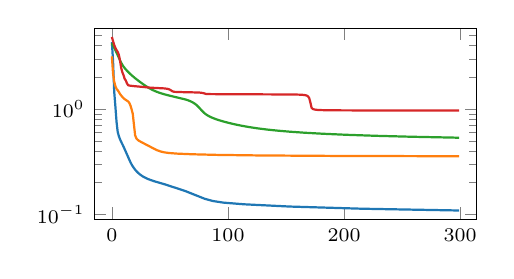
\begin{tikzpicture}

\definecolor{crimson2143940}{RGB}{214,39,40}
\definecolor{darkgray176}{RGB}{176,176,176}
\definecolor{darkorange25512714}{RGB}{255,127,14}
\definecolor{forestgreen4416044}{RGB}{44,160,44}
\definecolor{steelblue31119180}{RGB}{31,119,180}

\begin{axis}[compar,
	ymode=log]
\addplot [thick, steelblue31119180]
table {%
0 4.31118011474609
1 2.86087012290955
2 1.46213376522064
3 1.0652574300766
4 0.757783889770508
5 0.608149290084839
6 0.553772449493408
7 0.517727613449097
8 0.489268779754639
10 0.441203594207764
14 0.350765705108643
15 0.330757141113281
16 0.313158273696899
17 0.298194766044617
18 0.285662889480591
20 0.266182661056519
22 0.251716256141663
24 0.240591883659363
27 0.228317499160767
31 0.217189311981201
36 0.207478642463684
46 0.192617893218994
63 0.167274951934814
80 0.140859723091125
87 0.134231090545654
96 0.129587531089783
114 0.124923467636108
153 0.118964076042175
215 0.113466620445251
299 0.109116911888123
};
\addplot [thick, darkorange25512714]
table {%
0 3.16804385185242
1 2.1728253364563
2 1.81974112987518
3 1.65217316150665
4 1.55622470378876
5 1.50949347019196
6 1.4545316696167
7 1.39175379276276
8 1.34442985057831
9 1.30509471893311
10 1.26971399784088
11 1.24319803714752
14 1.18106353282928
15 1.14478838443756
16 1.07928073406219
17 0.99414074420929
18 0.899261236190796
19 0.711821794509888
20 0.564864158630371
21 0.529275417327881
22 0.51323676109314
23 0.502990245819092
25 0.488440990447998
36 0.422354698181152
39 0.407036423683167
42 0.396010875701904
45 0.388900637626648
49 0.383358359336853
56 0.37813663482666
69 0.372749328613281
91 0.36762523651123
127 0.363221168518066
190 0.359556078910828
299 0.356795787811279
};
\addplot [thick, forestgreen4416044]
table {%
0 4.22285127639771
1 4.01487064361572
2 3.81293964385986
3 3.61843371391296
4 3.43001246452332
5 3.24553966522217
6 3.06602549552917
7 2.89872932434082
8 2.75325393676758
9 2.63300466537476
10 2.53405690193176
11 2.45044136047363
12 2.37739825248718
13 2.31180191040039
14 2.2517294883728
15 2.19601726531982
16 2.14395308494568
17 2.09506845474243
18 2.04901480674744
19 2.00549292564392
20 1.96422600746155
22 1.88743078708649
24 1.81681656837463
26 1.75109088420868
28 1.68976640701294
30 1.63334107398987
32 1.58285140991211
34 1.53889524936676
36 1.50113666057587
38 1.46864080429077
40 1.44038474559784
42 1.41550385951996
45 1.38306832313538
48 1.35499906539917
52 1.32209038734436
63 1.23652398586273
65 1.21735787391663
67 1.1948823928833
69 1.16740524768829
70 1.15111398696899
71 1.13272404670715
72 1.11198115348816
73 1.08876585960388
75 1.03586375713348
77 0.979917526245117
78 0.953849077224731
79 0.93034839630127
80 0.909757375717163
81 0.89196240901947
82 0.876595616340637
84 0.851416349411011
86 0.831281900405884
89 0.80668306350708
92 0.786139488220215
96 0.762671232223511
101 0.737642288208008
106 0.716179132461548
112 0.694188952445984
118 0.675628066062927
125 0.657562732696533
133 0.640705108642578
142 0.625406861305237
153 0.610499143600464
166 0.596593141555786
182 0.583184480667114
202 0.570235252380371
227 0.557931184768677
258 0.54643702507019
299 0.534921646118164
};
\addplot [thick, crimson2143940]
table {%
0 4.83801460266113
1 4.40892267227173
2 4.0575966835022
3 3.81000995635986
4 3.62662363052368
5 3.4903404712677
6 3.26991677284241
7 2.88387107849121
8 2.46064591407776
9 2.23875594139099
10 2.09848737716675
11 1.93832695484161
12 1.86550188064575
13 1.75230574607849
14 1.68575251102448
15 1.67313063144684
16 1.66563010215759
18 1.65520441532135
22 1.63989841938019
27 1.62095606327057
32 1.5998467206955
35 1.59214544296265
45 1.57121884822845
47 1.56174802780151
48 1.55420339107513
49 1.54314243793488
50 1.52653920650482
52 1.47822439670563
53 1.46314704418182
54 1.45740079879761
56 1.45306062698364
61 1.44800436496735
74 1.43711578845978
76 1.43223798274994
78 1.42263174057007
79 1.4143158197403
81 1.39276945590973
82 1.3884299993515
86 1.38631105422974
103 1.38339865207672
155 1.37558126449585
161 1.37109315395355
164 1.36570847034454
166 1.35810971260071
167 1.351198554039
168 1.3394980430603
169 1.31697833538055
170 1.26625549793243
171 1.14868927001953
172 1.02802407741547
173 1.00346457958221
174 0.994166612625122
175 0.988674879074097
177 0.982434272766113
180 0.978082180023193
186 0.974670767784119
199 0.972140312194824
233 0.970206499099731
299 0.969050168991089
};
\end{axis}

\end{tikzpicture}
}
&
\multicolumn{4}{c}{% This file was created with tikzplotlib v0.10.1.
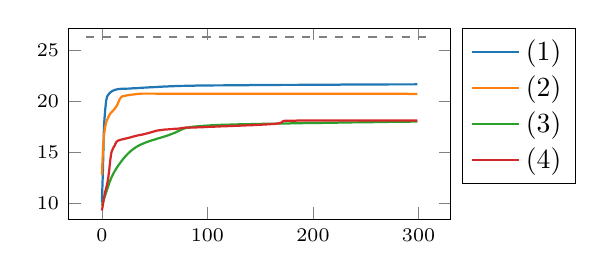
\begin{tikzpicture}

\definecolor{crimson2143940}{RGB}{214,39,40}
\definecolor{darkgray176}{RGB}{176,176,176}
\definecolor{darkorange25512714}{RGB}{255,127,14}
\definecolor{forestgreen4416044}{RGB}{44,160,44}
\definecolor{steelblue31119180}{RGB}{31,119,180}

\begin{axis}[compar, legend pos=outer north east]
\addplot [thick, steelblue31119180]
table {%
0 10.0600004196167
1 13.2399997711182
2 17.6399993896484
3 19.0200004577637
4 20.0400009155273
5 20.4799995422363
6 20.6399993896484
7 20.7700004577637
8 20.8799991607666
9 20.9599990844727
10 21.0200004577637
11 21.0699996948242
13 21.1499996185303
14 21.1700000762939
15 21.2000007629395
18 21.2299995422363
20 21.2299995422363
21 21.2399997711182
23 21.2399997711182
24 21.25
25 21.25
26 21.2600002288818
27 21.2600002288818
29 21.2800006866455
30 21.2800006866455
31 21.2900009155273
32 21.2900009155273
34 21.3099994659424
35 21.3099994659424
37 21.3299999237061
38 21.3299999237061
40 21.3500003814697
41 21.3500003814697
42 21.3600006103516
43 21.3600006103516
45 21.3799991607666
46 21.3799991607666
47 21.3899993896484
48 21.3899993896484
49 21.3999996185303
50 21.3999996185303
52 21.4200000762939
53 21.4200000762939
54 21.4300003051758
55 21.4300003051758
56 21.4400005340576
57 21.4400005340576
58 21.4500007629395
59 21.4500007629395
60 21.4599990844727
61 21.4599990844727
62 21.4699993133545
63 21.4699993133545
64 21.4799995422363
65 21.4799995422363
66 21.4899997711182
68 21.4899997711182
69 21.5
71 21.5
72 21.5100002288818
74 21.5100002288818
75 21.5200004577637
78 21.5200004577637
79 21.5300006866455
82 21.5300006866455
83 21.5400009155273
88 21.5400009155273
89 21.5499992370605
96 21.5499992370605
97 21.5599994659424
105 21.5599994659424
106 21.5699996948242
115 21.5699996948242
116 21.5799999237061
126 21.5799999237061
127 21.5900001525879
139 21.5900001525879
140 21.6000003814697
153 21.6000003814697
154 21.6100006103516
169 21.6100006103516
170 21.6200008392334
186 21.6200008392334
187 21.6299991607666
205 21.6299991607666
206 21.6399993896484
226 21.6399993896484
227 21.6499996185303
248 21.6499996185303
249 21.6599998474121
271 21.6599998474121
272 21.6700000762939
296 21.6700000762939
297 21.6800003051758
299 21.6800003051758
};
\addlegendentry{$(1)$}
\addplot [thick, darkorange25512714]
table {%
0 12.7600002288818
1 15.289999961853
2 16.6800003051758
3 17.4300003051758
4 17.9300003051758
5 18.2000007629395
6 18.4300003051758
7 18.6399993896484
8 18.8099994659424
9 18.9300003051758
10 19.0300006866455
11 19.1399993896484
12 19.2600002288818
13 19.3999996185303
14 19.5499992370605
15 19.75
16 20.0100002288818
17 20.25
18 20.3700008392334
19 20.4799995422363
20 20.5100002288818
25 20.6100006103516
26 20.6200008392334
27 20.6399993896484
28 20.6499996185303
29 20.6700000762939
31 20.6900005340576
32 20.7099990844727
36 20.75
37 20.75
38 20.7600002288818
51 20.7600002288818
52 20.75
222 20.75
223 20.7399997711182
290 20.7399997711182
291 20.7299995422363
299 20.7299995422363
};
\addlegendentry{$(2)$}
\addplot [thick, forestgreen4416044]
table {%
0 9.77999973297119
1 10.1099996566772
3 10.75
4 11.0600004196167
5 11.3800001144409
6 11.6899995803833
7 11.9899997711182
8 12.2700004577637
9 12.5200004577637
10 12.7399997711182
11 12.9399995803833
12 13.1300001144409
14 13.4700002670288
15 13.6199998855591
16 13.7799997329712
17 13.9200000762939
18 14.0699996948242
21 14.460000038147
22 14.5799999237061
24 14.8000001907349
27 15.1000003814697
28 15.1800003051758
29 15.2700004577637
30 15.3400001525879
31 15.4200000762939
32 15.4899997711182
35 15.6700000762939
38 15.8199996948242
40 15.8999996185303
41 15.9499998092651
42 15.9899997711182
43 16.0200004577637
45 16.1000003814697
46 16.1299991607666
47 16.1700000762939
51 16.2900009155273
52 16.3299999237061
58 16.5100002288818
59 16.5499992370605
61 16.6100006103516
62 16.6499996185303
63 16.6800003051758
69 16.9200000762939
72 17.0699996948242
73 17.1100006103516
76 17.2600002288818
78 17.3400001525879
80 17.3999996185303
84 17.4799995422363
85 17.4899997711182
86 17.5100002288818
95 17.6000003814697
96 17.6000003814697
98 17.6200008392334
99 17.6200008392334
101 17.6399993896484
102 17.6399993896484
103 17.6499996185303
104 17.6499996185303
105 17.6599998474121
106 17.6599998474121
107 17.6700000762939
108 17.6700000762939
109 17.6800003051758
110 17.6800003051758
111 17.6900005340576
112 17.6900005340576
113 17.7000007629395
115 17.7000007629395
116 17.7099990844727
118 17.7099990844727
119 17.7199993133545
121 17.7199993133545
122 17.7299995422363
125 17.7299995422363
126 17.7399997711182
128 17.7399997711182
129 17.75
132 17.75
133 17.7600002288818
137 17.7600002288818
138 17.7700004577637
141 17.7700004577637
142 17.7800006866455
146 17.7800006866455
147 17.7900009155273
151 17.7900009155273
152 17.7999992370605
156 17.7999992370605
157 17.8099994659424
161 17.8099994659424
162 17.8199996948242
167 17.8199996948242
168 17.8299999237061
172 17.8299999237061
173 17.8400001525879
178 17.8400001525879
179 17.8500003814697
184 17.8500003814697
185 17.8600006103516
190 17.8600006103516
191 17.8700008392334
196 17.8700008392334
197 17.8799991607666
203 17.8799991607666
204 17.8899993896484
209 17.8899993896484
210 17.8999996185303
216 17.8999996185303
217 17.9099998474121
223 17.9099998474121
224 17.9200000762939
230 17.9200000762939
231 17.9300003051758
236 17.9300003051758
237 17.9400005340576
243 17.9400005340576
244 17.9500007629395
250 17.9500007629395
251 17.9599990844727
257 17.9599990844727
258 17.9699993133545
264 17.9699993133545
265 17.9799995422363
271 17.9799995422363
272 17.9899997711182
278 17.9899997711182
279 18
285 18
286 18.0100002288818
292 18.0100002288818
293 18.0200004577637
299 18.0200004577637
};
\addlegendentry{$(3)$}
\addplot [thick, crimson2143940]
table {%
0 9.30000019073486
1 9.85999965667725
2 10.539999961853
3 11.0600004196167
4 11.4799995422363
5 11.8900003433228
6 12.4700002670288
7 13.3000001907349
8 14.289999961853
9 14.9799995422363
10 15.25
11 15.4799995422363
12 15.6400003433228
13 15.8800001144409
14 16.0599994659424
15 16.1299991607666
16 16.1800003051758
19 16.2700004577637
20 16.2900009155273
21 16.3199996948242
22 16.3400001525879
23 16.3700008392334
24 16.3899993896484
25 16.4200000762939
26 16.4400005340576
30 16.5599994659424
31 16.5799999237061
33 16.6399993896484
39 16.7600002288818
40 16.7900009155273
41 16.8099994659424
42 16.8400001525879
43 16.8600006103516
52 17.1299991607666
53 17.1399993896484
54 17.1599998474121
55 17.1700000762939
56 17.1900005340576
57 17.2000007629395
58 17.2199993133545
60 17.2399997711182
61 17.2399997711182
65 17.2800006866455
66 17.2800006866455
70 17.3199996948242
71 17.3199996948242
74 17.3500003814697
75 17.3700008392334
76 17.3799991607666
77 17.3999996185303
78 17.4099998474121
79 17.4300003051758
80 17.4400005340576
81 17.4300003051758
82 17.4300003051758
83 17.4200000762939
84 17.4300003051758
87 17.4300003051758
88 17.4400005340576
89 17.4400005340576
90 17.4500007629395
91 17.4500007629395
92 17.4599990844727
94 17.4599990844727
95 17.4699993133545
96 17.4699993133545
97 17.4799995422363
98 17.4799995422363
99 17.4899997711182
100 17.4899997711182
101 17.5
103 17.5
104 17.5100002288818
105 17.5100002288818
106 17.5200004577637
107 17.5200004577637
108 17.5300006866455
110 17.5300006866455
111 17.5400009155273
112 17.5400009155273
113 17.5499992370605
114 17.5499992370605
115 17.5599994659424
117 17.5599994659424
118 17.5699996948242
119 17.5699996948242
120 17.5799999237061
122 17.5799999237061
123 17.5900001525879
124 17.5900001525879
125 17.6000003814697
126 17.6000003814697
127 17.6100006103516
129 17.6100006103516
130 17.6200008392334
131 17.6200008392334
132 17.6299991607666
134 17.6299991607666
135 17.6399993896484
136 17.6399993896484
137 17.6499996185303
138 17.6499996185303
139 17.6599998474121
141 17.6599998474121
142 17.6700000762939
143 17.6700000762939
144 17.6800003051758
145 17.6800003051758
146 17.6900005340576
147 17.6900005340576
148 17.7000007629395
149 17.7000007629395
150 17.7099990844727
151 17.7099990844727
152 17.7199993133545
153 17.7199993133545
154 17.7299995422363
155 17.7299995422363
157 17.75
158 17.75
161 17.7800006866455
162 17.7800006866455
165 17.8099994659424
166 17.8299999237061
167 17.8400001525879
169 17.8799991607666
170 17.9200000762939
171 18.0100002288818
172 18.0799999237061
174 18.1000003814697
176 18.1000003814697
177 18.1100006103516
184 18.1100006103516
185 18.1200008392334
260 18.1200008392334
261 18.1299991607666
299 18.1299991607666
};
\addlegendentry{$(4)$}
\addplot [thick, gray, dashed]
table {%
-14.95 26.3238544464111
313.95 26.3238544464111
};
\end{axis}

\end{tikzpicture}
}
\end{tabular}
    %\includegraphics[width=1.\textwidth]{../resultats/LGD/differentes initialisation/inits-s_multiplot.png}
    \caption{En première lignes différentes initialisation avec en dessous le résultats de la LGD après 300 itérations -- sans filtre passe-bas}
    \label{fig:LGDinits}
\end{figure}

\begin{figure}[H]\centering
    \begin{tabular}{c c c c c c}
	Target  &  $(1)$  &  $(2)$  &  $(3)$  &  $(4)$  &  $(5)$
	
	\\
	
	\multirow{3}{0.32\textwidth}[0.075\textwidth]{\includegraphics[width=0.32\textwidth]{resultats/LGD/sizes/size-target-g.png}}
	&
	\includegraphics[width=0.1\textwidth]{resultats/LGD/sizes/size_big-init-pas=0.2_filtre=g-0.6.png}
	&
	\includegraphics[width=0.1\textwidth]{resultats/LGD/sizes/size_mid2-init-pas=0.1_filtre=g-0.6.png}
	&
	\includegraphics[width=0.1\textwidth]{resultats/LGD/sizes/size_mid1-init-pas=0.1_filtre=g-0.6.png}
	&
	\includegraphics[width=0.1\textwidth]{resultats/LGD/sizes/size_small-init-pas=0.5_filtre=g-0.6.png}
	&
	\includegraphics[width=0.1\textwidth]{resultats/LGD/sizes/size_mini-init-pas=0.01_filtre=g-0.6.png}
	
	\\
	
	
	&
	\includegraphics[width=0.1\textwidth]{resultats/LGD/sizes/size_big-compatarget-s.png}
	&
	\includegraphics[width=0.1\textwidth]{resultats/LGD/sizes/size_mid2-compatarget-s.png}
	&
	\includegraphics[height=0.1\textwidth]{resultats/LGD/sizes/size_mid1-compatarget-s.png}
	&
	\includegraphics[width=0.1\textwidth]{resultats/LGD/sizes/size_small-compatarget-s.png}
	&
	\includegraphics[width=0.1\textwidth]{resultats/LGD/sizes/size_mini-compatarget-s.png}
	
	\\
	
	
	&
	\includegraphics[width=0.1\textwidth]{resultats/LGD/sizes/size_big-guess-pas=0.2_filtre=g-0.6.png}
	&
	\includegraphics[width=0.1\textwidth]{resultats/LGD/sizes/size_mid2-guess-pas=0.1_filtre=g-0.6.png}
	&
	\includegraphics[width=0.1\textwidth]{resultats/LGD/sizes/size_mid1-guess-pas=0.1_filtre=g-0.6.png}
	&
	\includegraphics[width=0.1\textwidth]{resultats/LGD/sizes/size_small-guess-pas=0.5_filtre=g-0.6.png}
	&
	\includegraphics[width=0.1\textwidth]{resultats/LGD/sizes/size_mini-guess-pas=0.01_filtre=g-0.6.png}
	
	\\ \\
	
	
	
	\multicolumn{2}{c}{Loss}  &  \multicolumn{4}{c}{PSNR{\color{white}bbbb}}
	
	\\
	
	\multicolumn{2}{c}{% This file was created with tikzplotlib v0.10.1.
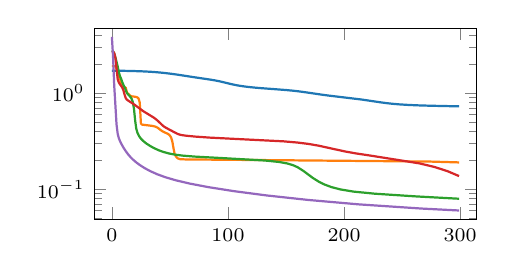
\begin{tikzpicture}

\definecolor{crimson2143940}{RGB}{214,39,40}
\definecolor{darkgray176}{RGB}{176,176,176}
\definecolor{darkorange25512714}{RGB}{255,127,14}
\definecolor{forestgreen4416044}{RGB}{44,160,44}
\definecolor{mediumpurple148103189}{RGB}{148,103,189}
\definecolor{steelblue31119180}{RGB}{31,119,180}

\begin{axis}[compar,
	ymode=log]
\addplot [thick, steelblue31119180]
table {%
0 1.72453677654266
10 1.71768462657928
18 1.709348320961
24 1.70033705234528
29 1.6901341676712
34 1.67662823200226
38 1.66295230388641
42 1.64652991294861
46 1.62746405601501
51 1.60032224655151
56 1.5699542760849
63 1.52379190921783
70 1.47829067707062
76 1.44239723682404
86 1.38365793228149
90 1.35641014575958
93 1.33313751220703
97 1.29875993728638
102 1.25543904304504
105 1.23231077194214
108 1.2123007774353
111 1.19530928134918
114 1.18089818954468
118 1.16483271121979
123 1.14839255809784
129 1.13209295272827
138 1.11113858222961
150 1.08306062221527
156 1.06606793403625
161 1.0491931438446
167 1.02564668655396
181 0.968385457992554
187 0.947251319885254
195 0.922387599945068
215 0.862796425819397
224 0.831477165222168
232 0.804347276687622
237 0.789946675300598
242 0.778159737586975
248 0.767242193222046
255 0.757997989654541
263 0.75055992603302
274 0.743492960929871
293 0.734858512878418
299 0.732345581054688
};
\addplot [thick, darkorange25512714]
table {%
0 1.93434596061707
1 1.93200349807739
2 1.92700910568237
3 1.91092967987061
4 1.82279932498932
5 1.63814675807953
6 1.49781715869904
7 1.42523396015167
8 1.27939009666443
9 1.18521678447723
10 1.17097330093384
11 1.16010677814484
12 1.13860154151917
13 1.018106341362
16 0.941693305969238
17 0.931789517402649
20 0.922242164611816
21 0.916382789611816
22 0.905909538269043
23 0.883619070053101
24 0.800576210021973
25 0.484217882156372
26 0.472478270530701
35 0.457828998565674
37 0.451737642288208
38 0.44725227355957
39 0.441246032714844
40 0.433329820632935
42 0.41453742980957
44 0.39980947971344
46 0.389489531517029
48 0.379505157470703
49 0.372840166091919
50 0.363147974014282
51 0.346918106079102
52 0.317295432090759
53 0.271204471588135
54 0.234548449516296
55 0.221139311790466
56 0.213874220848083
57 0.209440231323242
59 0.205981850624084
64 0.20487642288208
108 0.202854156494141
273 0.194810152053833
297 0.191097617149353
299 0.190571308135986
};
\addplot [thick, forestgreen4416044]
table {%
0 2.80895972251892
1 2.75048971176147
2 2.60713028907776
3 2.38255786895752
4 2.13562965393066
5 1.91229856014252
6 1.65637183189392
7 1.50856399536133
8 1.41280651092529
9 1.30485808849335
10 1.22169101238251
11 1.15476989746094
12 1.0741560459137
13 1.00716495513916
14 0.973587155342102
15 0.946269989013672
16 0.916436076164246
17 0.876654148101807
18 0.812723636627197
19 0.697008371353149
20 0.525444269180298
21 0.428455829620361
22 0.389726042747498
23 0.366618156433105
24 0.350306034088135
25 0.337761163711548
26 0.32756519317627
28 0.311413407325745
30 0.298583030700684
33 0.282851934432983
36 0.269976496696472
40 0.256317496299744
44 0.245958089828491
49 0.236628293991089
54 0.230266451835632
61 0.224518775939941
71 0.219510316848755
92 0.2126624584198
132 0.199638366699219
144 0.192842841148376
151 0.186120629310608
156 0.178535461425781
160 0.169811010360718
165 0.155425310134888
173 0.131635665893555
178 0.120536088943481
183 0.112421870231628
189 0.10558009147644
197 0.0996513366699219
208 0.0947535037994385
226 0.0901226997375488
262 0.0843832492828369
299 0.0798095464706421
};
\addplot [thick, crimson2143940]
table {%
0 2.75355887413025
1 2.72030234336853
2 2.63165354728699
3 2.34783864021301
4 1.81270730495453
5 1.40633320808411
6 1.2964209318161
7 1.23945200443268
8 1.19617938995361
9 1.146324634552
10 1.06876111030579
11 0.963654279708862
12 0.885666608810425
13 0.858596682548523
14 0.841736435890198
20 0.754436254501343
24 0.694417476654053
26 0.666041374206543
28 0.641217947006226
30 0.620044827461243
36 0.559826135635376
38 0.536990165710449
40 0.511477112770081
43 0.471526265144348
44 0.459928154945374
45 0.450082421302795
47 0.435087561607361
56 0.381032824516296
58 0.372854471206665
60 0.367727637290955
64 0.361920237541199
72 0.354321241378784
84 0.346086740493774
101 0.337772607803345
148 0.316205859184265
160 0.30713939666748
169 0.297676563262939
178 0.285158157348633
191 0.26324725151062
201 0.247857093811035
210 0.236915230751038
223 0.224390149116516
265 0.186241030693054
278 0.17077362537384
289 0.154715538024902
299 0.137419939041138
};
\addplot [thick, mediumpurple148103189]
table {%
0 3.87609815597534
1 2.41971015930176
2 1.21478092670441
3 0.759954929351807
4 0.473417043685913
5 0.378544330596924
6 0.340376138687134
7 0.318324327468872
8 0.300664186477661
9 0.285422086715698
10 0.271982550621033
12 0.249404191970825
14 0.231428861618042
16 0.216980695724487
18 0.205150842666626
21 0.190834045410156
24 0.179333209991455
28 0.166966199874878
33 0.154839515686035
39 0.143672823905945
46 0.133790850639343
55 0.124259471893311
67 0.114835143089294
83 0.105466246604919
105 0.0957608222961426
133 0.0864417552947998
169 0.0775313377380371
213 0.0696594715118408
267 0.0630255937576294
299 0.0601816177368164
};
\end{axis}

\end{tikzpicture}
}
	&
	\multicolumn{4}{c}{% This file was created with tikzplotlib v0.10.1.
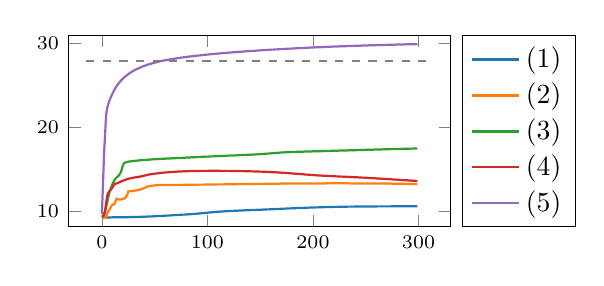
\begin{tikzpicture}

\definecolor{crimson2143940}{RGB}{214,39,40}
\definecolor{darkgray176}{RGB}{176,176,176}
\definecolor{darkorange25512714}{RGB}{255,127,14}
\definecolor{forestgreen4416044}{RGB}{44,160,44}
\definecolor{mediumpurple148103189}{RGB}{148,103,189}
\definecolor{steelblue31119180}{RGB}{31,119,180}

\begin{axis}[compar, legend pos=outer north east]
\addplot [thick, steelblue31119180]
table {%
0 9.31999969482422
9 9.31999969482422
10 9.32999992370605
17 9.32999992370605
18 9.34000015258789
22 9.34000015258789
23 9.35000038146973
26 9.35000038146973
27 9.35999965667725
30 9.35999965667725
31 9.36999988555908
33 9.36999988555908
34 9.38000011444092
36 9.38000011444092
37 9.39000034332275
38 9.39000034332275
39 9.39999961853027
40 9.39999961853027
41 9.40999984741211
42 9.40999984741211
43 9.42000007629395
44 9.42000007629395
45 9.43000030517578
46 9.43000030517578
47 9.4399995803833
48 9.4399995803833
49 9.44999980926514
50 9.44999980926514
52 9.47000026702881
53 9.47000026702881
55 9.48999977111816
56 9.48999977111816
58 9.51000022888184
59 9.51000022888184
61 9.52999973297119
62 9.52999973297119
65 9.5600004196167
66 9.5600004196167
69 9.59000015258789
70 9.59000015258789
73 9.61999988555908
74 9.61999988555908
77 9.64999961853027
78 9.64999961853027
82 9.6899995803833
83 9.6899995803833
94 9.80000019073486
95 9.81999969482422
98 9.85000038146973
99 9.86999988555908
103 9.90999984741211
104 9.93000030517578
112 10.0100002288818
113 10.0100002288818
117 10.0500001907349
118 10.0500001907349
120 10.0699996948242
121 10.0699996948242
123 10.0900001525879
124 10.0900001525879
126 10.1099996566772
127 10.1099996566772
128 10.1199998855591
129 10.1199998855591
130 10.1300001144409
131 10.1300001144409
133 10.1499996185303
134 10.1499996185303
135 10.1599998474121
136 10.1599998474121
137 10.1700000762939
138 10.1700000762939
139 10.1800003051758
140 10.1800003051758
141 10.1899995803833
142 10.1899995803833
143 10.1999998092651
144 10.1999998092651
145 10.210000038147
146 10.210000038147
147 10.2200002670288
148 10.2200002670288
149 10.2299995422363
150 10.2299995422363
151 10.2399997711182
152 10.2399997711182
153 10.25
154 10.25
155 10.2600002288818
156 10.2600002288818
157 10.2700004577637
158 10.2700004577637
159 10.2799997329712
160 10.2799997329712
161 10.289999961853
162 10.289999961853
164 10.3100004196167
165 10.3100004196167
166 10.3199996948242
167 10.3199996948242
168 10.3299999237061
169 10.3299999237061
171 10.3500003814697
172 10.3500003814697
173 10.3599996566772
174 10.3599996566772
175 10.3699998855591
176 10.3699998855591
178 10.3900003433228
179 10.3900003433228
180 10.3999996185303
181 10.3999996185303
182 10.4099998474121
183 10.4099998474121
184 10.4200000762939
185 10.4200000762939
186 10.4300003051758
187 10.4300003051758
188 10.4399995803833
189 10.4399995803833
190 10.4499998092651
191 10.4499998092651
192 10.460000038147
193 10.460000038147
194 10.4700002670288
195 10.4700002670288
196 10.4799995422363
197 10.4799995422363
198 10.4899997711182
200 10.4899997711182
201 10.5
202 10.5
203 10.5100002288818
205 10.5100002288818
206 10.5200004577637
207 10.5200004577637
208 10.5299997329712
210 10.5299997329712
211 10.539999961853
213 10.539999961853
214 10.5500001907349
216 10.5500001907349
217 10.5600004196167
219 10.5600004196167
220 10.5699996948242
223 10.5699996948242
224 10.5799999237061
227 10.5799999237061
228 10.5900001525879
232 10.5900001525879
233 10.6000003814697
239 10.6000003814697
240 10.6099996566772
248 10.6099996566772
249 10.6199998855591
260 10.6199998855591
261 10.6300001144409
274 10.6300001144409
275 10.6400003433228
287 10.6400003433228
288 10.6499996185303
299 10.6499996185303
};
\addlegendentry{$(1)$}
\addplot [thick, darkorange25512714]
table {%
0 9.28999996185303
1 9.28999996185303
2 9.30000019073486
3 9.31999969482422
4 9.4399995803833
5 9.73999977111816
6 10.0600004196167
7 10.1899995803833
8 10.4499998092651
9 10.6599998474121
10 10.8100004196167
11 10.8400001525879
12 10.9200000762939
13 11.2200002670288
14 11.5500001907349
15 11.5100002288818
16 11.460000038147
17 11.4399995803833
18 11.460000038147
19 11.4700002670288
20 11.5100002288818
21 11.5600004196167
22 11.6400003433228
23 11.75
24 12.0100002288818
25 12.3999996185303
26 12.4099998474121
27 12.4499998092651
28 12.4300003051758
29 12.4700002670288
30 12.460000038147
31 12.5
32 12.5
33 12.539999961853
34 12.5500001907349
35 12.5900001525879
36 12.6099996566772
37 12.6599998474121
38 12.6899995803833
40 12.789999961853
41 12.8599996566772
43 12.960000038147
44 13
45 13.0200004577637
46 13.0500001907349
47 13.0699996948242
48 13.0799999237061
50 13.1199998855591
51 13.1300001144409
52 13.1499996185303
53 13.1499996185303
54 13.1599998474121
60 13.1599998474121
61 13.1700000762939
69 13.1700000762939
70 13.1800003051758
77 13.1800003051758
78 13.1899995803833
84 13.1899995803833
85 13.1999998092651
91 13.1999998092651
92 13.210000038147
97 13.210000038147
98 13.2200002670288
104 13.2200002670288
105 13.2299995422363
109 13.2299995422363
110 13.2399997711182
115 13.2399997711182
116 13.25
121 13.25
122 13.2600002288818
127 13.2600002288818
128 13.2700004577637
133 13.2700004577637
134 13.2799997329712
139 13.2799997329712
140 13.289999961853
146 13.289999961853
147 13.3000001907349
153 13.3000001907349
154 13.3100004196167
160 13.3100004196167
161 13.3199996948242
168 13.3199996948242
169 13.3299999237061
178 13.3299999237061
179 13.3400001525879
190 13.3400001525879
191 13.3500003814697
211 13.3500003814697
212 13.3599996566772
234 13.3599996566772
235 13.3500003814697
255 13.3500003814697
256 13.3400001525879
266 13.3400001525879
267 13.3299999237061
274 13.3299999237061
275 13.3199996948242
280 13.3199996948242
281 13.3100004196167
285 13.3100004196167
286 13.3000001907349
289 13.3000001907349
290 13.289999961853
293 13.289999961853
294 13.2799997329712
296 13.2799997329712
297 13.2700004577637
299 13.2700004577637
};
\addlegendentry{$(2)$}
\addplot [thick, forestgreen4416044]
table {%
0 9.39999961853027
1 9.48999977111816
2 9.69999980926514
3 10.0799999237061
4 10.539999961853
5 11.039999961853
6 11.6999998092651
7 12.1999998092651
8 12.5699996948242
9 12.9499998092651
10 13.2600002288818
12 13.7399997711182
13 13.9399995803833
14 14.0600004196167
15 14.1700000762939
16 14.289999961853
17 14.460000038147
18 14.710000038147
19 15.0900001525879
20 15.5299997329712
21 15.7399997711182
22 15.8199996948242
23 15.8699998855591
25 15.9300003051758
27 15.9700002670288
28 15.9799995422363
29 16
30 16.0100002288818
31 16.0300006866455
33 16.0499992370605
34 16.0699996948242
48 16.2099990844727
49 16.2099990844727
52 16.2399997711182
53 16.2399997711182
55 16.2600002288818
56 16.2600002288818
58 16.2800006866455
59 16.2800006866455
61 16.2999992370605
62 16.2999992370605
63 16.3099994659424
64 16.3099994659424
66 16.3299999237061
67 16.3299999237061
69 16.3500003814697
70 16.3500003814697
72 16.3700008392334
73 16.3700008392334
74 16.3799991607666
75 16.3799991607666
77 16.3999996185303
78 16.3999996185303
80 16.4200000762939
81 16.4200000762939
82 16.4300003051758
83 16.4300003051758
85 16.4500007629395
86 16.4500007629395
87 16.4599990844727
88 16.4599990844727
90 16.4799995422363
91 16.4799995422363
92 16.4899997711182
93 16.4899997711182
95 16.5100002288818
96 16.5100002288818
97 16.5200004577637
98 16.5200004577637
99 16.5300006866455
100 16.5300006866455
102 16.5499992370605
103 16.5499992370605
104 16.5599994659424
105 16.5599994659424
106 16.5699996948242
107 16.5699996948242
109 16.5900001525879
110 16.5900001525879
111 16.6000003814697
112 16.6000003814697
113 16.6100006103516
114 16.6100006103516
115 16.6200008392334
116 16.6200008392334
118 16.6399993896484
119 16.6399993896484
120 16.6499996185303
121 16.6499996185303
122 16.6599998474121
123 16.6599998474121
124 16.6700000762939
125 16.6700000762939
126 16.6800003051758
127 16.6800003051758
129 16.7000007629395
130 16.7000007629395
131 16.7099990844727
132 16.7099990844727
133 16.7199993133545
134 16.7199993133545
135 16.7299995422363
136 16.7299995422363
138 16.75
139 16.75
140 16.7600002288818
141 16.7600002288818
143 16.7800006866455
144 16.7800006866455
146 16.7999992370605
147 16.7999992370605
150 16.8299999237061
151 16.8299999237061
169 17.0100002288818
170 17.0100002288818
173 17.0400009155273
174 17.0400009155273
176 17.0599994659424
177 17.0599994659424
178 17.0699996948242
179 17.0699996948242
180 17.0799999237061
181 17.0799999237061
182 17.0900001525879
183 17.0900001525879
184 17.1000003814697
186 17.1000003814697
187 17.1100006103516
188 17.1100006103516
189 17.1200008392334
191 17.1200008392334
192 17.1299991607666
194 17.1299991607666
195 17.1399993896484
197 17.1399993896484
198 17.1499996185303
199 17.1499996185303
200 17.1599998474121
202 17.1599998474121
203 17.1700000762939
205 17.1700000762939
206 17.1800003051758
208 17.1800003051758
209 17.1900005340576
211 17.1900005340576
212 17.2000007629395
214 17.2000007629395
215 17.2099990844727
216 17.2099990844727
217 17.2199993133545
219 17.2199993133545
220 17.2299995422363
222 17.2299995422363
223 17.2399997711182
224 17.2399997711182
225 17.25
227 17.25
228 17.2600002288818
230 17.2600002288818
231 17.2700004577637
233 17.2700004577637
234 17.2800006866455
235 17.2800006866455
236 17.2900009155273
238 17.2900009155273
239 17.2999992370605
241 17.2999992370605
242 17.3099994659424
243 17.3099994659424
244 17.3199996948242
246 17.3199996948242
247 17.3299999237061
249 17.3299999237061
250 17.3400001525879
252 17.3400001525879
253 17.3500003814697
255 17.3500003814697
256 17.3600006103516
257 17.3600006103516
258 17.3700008392334
260 17.3700008392334
261 17.3799991607666
263 17.3799991607666
264 17.3899993896484
266 17.3899993896484
267 17.3999996185303
269 17.3999996185303
270 17.4099998474121
272 17.4099998474121
273 17.4200000762939
275 17.4200000762939
276 17.4300003051758
278 17.4300003051758
279 17.4400005340576
281 17.4400005340576
282 17.4500007629395
284 17.4500007629395
285 17.4599990844727
287 17.4599990844727
288 17.4699993133545
291 17.4699993133545
292 17.4799995422363
294 17.4799995422363
295 17.4899997711182
297 17.4899997711182
298 17.5
299 17.5
};
\addlegendentry{$(3)$}
\addplot [thick, crimson2143940]
table {%
0 9.38000011444092
1 9.4399995803833
2 9.59000015258789
3 10.039999961853
4 11
5 11.8900003433228
6 12.210000038147
7 12.3999996185303
8 12.539999961853
9 12.6899995803833
10 12.8800001144409
11 13.1000003814697
12 13.25
13 13.3100004196167
17 13.5100002288818
18 13.5699996948242
19 13.6199998855591
20 13.6800003051758
22 13.7799997329712
25 13.8999996185303
28 13.9899997711182
29 14.0100002288818
30 14.039999961853
37 14.1800003051758
44 14.3900003433228
50 14.5100002288818
51 14.5200004577637
53 14.5600004196167
54 14.5699996948242
55 14.5900001525879
56 14.6000003814697
57 14.6199998855591
69 14.7399997711182
70 14.7399997711182
72 14.7600002288818
73 14.7600002288818
75 14.7799997329712
76 14.7799997329712
77 14.789999961853
78 14.789999961853
79 14.8000001907349
81 14.8000001907349
82 14.8100004196167
84 14.8100004196167
85 14.8199996948242
87 14.8199996948242
88 14.8299999237061
92 14.8299999237061
93 14.8400001525879
100 14.8400001525879
101 14.8500003814697
111 14.8500003814697
112 14.8400001525879
121 14.8400001525879
122 14.8299999237061
126 14.8299999237061
127 14.8199996948242
131 14.8199996948242
132 14.8100004196167
135 14.8100004196167
136 14.8000001907349
138 14.8000001907349
139 14.789999961853
141 14.789999961853
142 14.7799997329712
144 14.7799997329712
145 14.7700004577637
146 14.7700004577637
147 14.7600002288818
149 14.7600002288818
150 14.75
151 14.75
152 14.7399997711182
153 14.7399997711182
154 14.7299995422363
155 14.7299995422363
156 14.7200002670288
157 14.7200002670288
158 14.710000038147
159 14.710000038147
161 14.6899995803833
162 14.6899995803833
164 14.6700000762939
165 14.6700000762939
167 14.6499996185303
168 14.6499996185303
172 14.6099996566772
173 14.6099996566772
200 14.3400001525879
201 14.3400001525879
205 14.3000001907349
206 14.3000001907349
209 14.2700004577637
210 14.2700004577637
212 14.25
213 14.25
215 14.2299995422363
216 14.2299995422363
217 14.2200002670288
218 14.2200002670288
220 14.1999998092651
221 14.1999998092651
222 14.1899995803833
223 14.1899995803833
224 14.1800003051758
225 14.1800003051758
227 14.1599998474121
228 14.1599998474121
229 14.1499996185303
230 14.1499996185303
231 14.1400003433228
232 14.1400003433228
234 14.1199998855591
235 14.1199998855591
236 14.1099996566772
237 14.1099996566772
239 14.0900001525879
240 14.0900001525879
241 14.0799999237061
242 14.0799999237061
244 14.0600004196167
245 14.0600004196167
247 14.039999961853
248 14.039999961853
250 14.0200004577637
251 14.0200004577637
254 13.9899997711182
255 13.9899997711182
257 13.9700002670288
258 13.9700002670288
262 13.9300003051758
263 13.9300003051758
266 13.8999996185303
267 13.8999996185303
271 13.8599996566772
272 13.8599996566772
276 13.8199996948242
277 13.8199996948242
282 13.7700004577637
283 13.7700004577637
286 13.7399997711182
287 13.7399997711182
291 13.6999998092651
292 13.6999998092651
295 13.6700000762939
296 13.6700000762939
298 13.6499996185303
299 13.6499996185303
};
\addlegendentry{$(4)$}
\addplot [thick, mediumpurple148103189]
table {%
0 9.72999954223633
1 13.0900001525879
2 16.6800003051758
3 19.1000003814697
4 21.4699993133545
5 22.2900009155273
6 22.7399997711182
7 23.1100006103516
8 23.4300003051758
9 23.7299995422363
10 24.0100002288818
11 24.2600002288818
12 24.4899997711182
13 24.7099990844727
14 24.8999996185303
15 25.0799999237061
16 25.25
17 25.3999996185303
19 25.6800003051758
21 25.9200000762939
22 26.0300006866455
24 26.2299995422363
26 26.4099998474121
29 26.6499996185303
31 26.7900009155273
32 26.8500003814697
33 26.9200000762939
35 27.0400009155273
37 27.1399993896484
38 27.2000007629395
39 27.25
40 27.2900009155273
41 27.3400001525879
43 27.4200000762939
44 27.4699993133545
45 27.5
47 27.5799999237061
48 27.6100006103516
49 27.6499996185303
51 27.7099990844727
52 27.75
54 27.8099994659424
55 27.8299999237061
57 27.8899993896484
58 27.9099998474121
60 27.9699993133545
62 28.0100002288818
63 28.0400009155273
75 28.2800006866455
76 28.2900009155273
79 28.3500003814697
80 28.3600006103516
81 28.3799991607666
82 28.3899993896484
83 28.4099998474121
84 28.4200000762939
85 28.4400005340576
86 28.4500007629395
87 28.4699993133545
88 28.4799995422363
89 28.5
90 28.5100002288818
91 28.5300006866455
93 28.5499992370605
94 28.5699996948242
96 28.5900001525879
97 28.6100006103516
100 28.6399993896484
101 28.6599998474121
105 28.7000007629395
106 28.7199993133545
112 28.7800006866455
113 28.7999992370605
132 28.9899997711182
133 28.9899997711182
141 29.0699996948242
142 29.0699996948242
148 29.1299991607666
149 29.1299991607666
153 29.1700000762939
154 29.1700000762939
157 29.2000007629395
158 29.2000007629395
161 29.2299995422363
162 29.2299995422363
165 29.2600002288818
166 29.2600002288818
169 29.2900009155273
170 29.2900009155273
172 29.3099994659424
173 29.3099994659424
175 29.3299999237061
176 29.3299999237061
178 29.3500003814697
179 29.3500003814697
181 29.3700008392334
182 29.3700008392334
184 29.3899993896484
185 29.3899993896484
187 29.4099998474121
188 29.4099998474121
190 29.4300003051758
191 29.4300003051758
192 29.4400005340576
193 29.4400005340576
195 29.4599990844727
196 29.4599990844727
197 29.4699993133545
198 29.4699993133545
199 29.4799995422363
200 29.4799995422363
202 29.5
203 29.5
204 29.5100002288818
205 29.5100002288818
206 29.5200004577637
207 29.5200004577637
208 29.5300006866455
209 29.5300006866455
210 29.5400009155273
211 29.5400009155273
213 29.5599994659424
214 29.5599994659424
215 29.5699996948242
216 29.5699996948242
217 29.5799999237061
218 29.5799999237061
219 29.5900001525879
220 29.5900001525879
221 29.6000003814697
222 29.6000003814697
223 29.6100006103516
224 29.6100006103516
225 29.6200008392334
227 29.6200008392334
228 29.6299991607666
229 29.6299991607666
230 29.6399993896484
231 29.6399993896484
232 29.6499996185303
233 29.6499996185303
234 29.6599998474121
235 29.6599998474121
236 29.6700000762939
238 29.6700000762939
239 29.6800003051758
240 29.6800003051758
241 29.6900005340576
242 29.6900005340576
243 29.7000007629395
245 29.7000007629395
246 29.7099990844727
247 29.7099990844727
248 29.7199993133545
250 29.7199993133545
251 29.7299995422363
252 29.7299995422363
253 29.7399997711182
255 29.7399997711182
256 29.75
258 29.75
259 29.7600002288818
260 29.7600002288818
261 29.7700004577637
263 29.7700004577637
264 29.7800006866455
266 29.7800006866455
267 29.7900009155273
269 29.7900009155273
270 29.7999992370605
272 29.7999992370605
273 29.8099994659424
275 29.8099994659424
276 29.8199996948242
278 29.8199996948242
279 29.8299999237061
281 29.8299999237061
282 29.8400001525879
284 29.8400001525879
285 29.8500003814697
287 29.8500003814697
288 29.8600006103516
291 29.8600006103516
292 29.8700008392334
294 29.8700008392334
295 29.8799991607666
298 29.8799991607666
299 29.8899993896484
};
\addlegendentry{$(5)$}
\addplot [thick, gray, dashed]
table {%
-14.95 27.8502388000488
313.95 27.8502388000488
};
\end{axis}

\end{tikzpicture}
}
\end{tabular}
    %\includegraphics[width=1.\textwidth]{../resultats/LGD/differentes initialisation/inits-g_multiplot.png}
    \caption{En première lignes différentes initialisation avec en dessous le résultats de la LGD après 300 itérations --  avec passe-bas gaussien ($\sigma=0.5$)}
    \label{fig:LGDinitg}
\end{figure}

Il va de soit que le calcul de PSNR est à but purement indicatif et n'intervient pas dans la LGD elle-même. Les ligne en pointillé représentent PSNR$\big(\bf{x_0},f(\bf{x_0})\big)$, le PSNR entre la cible $\bf{x_0}$ est sa version auto-encodée.
Dans la première figure \textit{\ref{fig:LGDinits}} il n'y pas de filtre passe-bas (\ei $A=S$) et dans la seconde \textit{\ref{fig:LGDinitg}}, $C_{\bf{h}}$ est un filtre gaussien de paramètre $\sigma=0.6$ (voir section \ref{sec:forma2pb} pour un rappel sur $\sigma$).
\\
Les différentes initialisations sont les suivantes :
\begin{enumerate}[label=(\arabic*)]
    \item $\bf{u_0}=f_E(^tA\bf{y_0})$, la backprojection encodée de $\bf{y_0}$
    \item $\bf{u_0}=f_E(\bf{x_0})+e$, l'image cible encodée puis bruité (bruit uniforme sur $]-0.5,0.5[$)
    \item idem, avec un bruit gaussien d'écart-type $0.5$
    \item $\bf{u_0}=\bf{u}_{\text{rand}}$,  vecteur aléatoire de l'espace latent
\end{enumerate}

\noindent La première initialisation est la plus naturelle puisqu'elle utilise $^tA$, ce qui se rapproche le plus d'un inverse pour $A$ (voir figure \textit{\ref{fig:passebas-g}} et \textit{\ref{fig:passebas-g}} en annexe \ref{anx:gradF} pour les visuels) et de même pour $f_E$ par rapport à $f_D$. 
\\
Les initialisations $(2)$ et $(3)$ sont au voisinage de de la cible  pour voir à quel point il possible de s'éloigner de $\bf{x_0}$ tout en conservant la convergence de l'algorithme.
\\

Cela étant dit, le premier constat est que la méthode fonctionne et ceux même en partant d'une vecteur aléatoire.  Aussi, même s'il sont meilleurs avec un passe-bas, les résultats restent satisfaisant sans filtre. La structure très simple du jeu de données aide probablement sur ce point et il serait intéressant de voir si les différences avec/sans filtre sont plus marqués sur un jeu de données plus complexe comme Fashion-MNIST.
\\
De plus, les courbes de loss de la figure \textit{\ref{fig:LGDinitg}} suggèrent que le résultats pourrait être améliorer avec plus d'itérations. Celles de la figure \textit{\ref{fig:LGDinits}} suggèrent une convergence mais comme  les courbes fond des saut, il possible que la loss puisse encore diminuer en échappant à ces plateaux. On pourrait par exemple ajouter de l'inertie à la descente.
\\
 
Autre chose remarquable, le résultats $(4)$ est meilleur que le $(3)$ alors que l'initialisation du premier est plus éloigné de la cible que le second. Cela est dû à la façon dont est tiré $\bf{u}_{\text{rand}}$. Pour rester cohérent avec la structure des images, et le réseau $f$ (composé de sigmoïde), les coefficients de $\bf{u}_{\text{rand}}$ sont tirés suivant une loi uniforme sur $[0,1]$. et l'auto encodeur gère très mal les vecteurs à valeurs trop loin de l'intervalle $[0,1]$. 
\\

Pour le voir, dans les figures \textit{\ref{fig:LGDgauss-s}} et \textit{\ref{fig:LGDgauss-g}} page suivante, chaque lignes correspond à un LGD avec en première ligne l'initialisation (décodée), en deuxième la reconstructions dont la cible est en troisième ligne. Les coefficients des initialisations sont tirés suivant une loi normal d'écart-type 2. En comparaison, les initialisations de la figure \textit{\ref{fig:LGDunif-g}} ci-dessous ont été tiré suivant une loi uniforme sur $[0,1]$. \textbf{\color{red}IL FAUT LES R2SULTATS...}

\textbf{\color{red}PENSES AU DIRE QUE CE A PAS CV MAIS QUE J4AI MIEUX A FOUTRE}

\begin{figure}[H]\centering
	\begin{tabular}{c c c c c c c c}
$(1)$  &  $(2)$  &  $(3)$  &  $(4)$  &  $(5)$  &  $(6)$  &  $(7)$  &  $(8)$
	
\\

\includegraphics[width=0.1\textwidth]{resultats/LGD/multitarget/unif_1-init-pas=0.25_filtre=g-0.6}
&
\includegraphics[width=0.1\textwidth]{resultats/LGD/multitarget/unif_2-init-pas=0.25_filtre=g-0.6}
&
\includegraphics[width=0.1\textwidth]{resultats/LGD/multitarget/unif_3-init-pas=0.25_filtre=g-0.6}
&
\includegraphics[width=0.1\textwidth]{resultats/LGD/multitarget/unif_4-init-pas=0.25_filtre=g-0.6}
&
\includegraphics[width=0.1\textwidth]{resultats/LGD/multitarget/unif_5-init-pas=0.25_filtre=g-0.6}
&
\includegraphics[width=0.1\textwidth]{resultats/LGD/multitarget/unif_6-init-pas=0.25_filtre=g-0.6}
&
\includegraphics[width=0.1\textwidth]{resultats/LGD/multitarget/unif_7-init-pas=0.25_filtre=g-0.6}
&
\includegraphics[width=0.1\textwidth]{resultats/LGD/multitarget/unif_8-init-pas=0.25_filtre=g-0.6}

\\

\includegraphics[width=0.1\textwidth]{resultats/LGD/multitarget/unif_1-guess-pas=0.25_filtre=g-0.6}
&
\includegraphics[width=0.1\textwidth]{resultats/LGD/multitarget/unif_2-guess-pas=0.25_filtre=g-0.6}
&
\includegraphics[width=0.1\textwidth]{resultats/LGD/multitarget/unif_3-guess-pas=0.25_filtre=g-0.6}
&
\includegraphics[width=0.1\textwidth]{resultats/LGD/multitarget/unif_4-guess-pas=0.25_filtre=g-0.6}
&
\includegraphics[width=0.1\textwidth]{resultats/LGD/multitarget/unif_5-guess-pas=0.25_filtre=g-0.6}
&
\includegraphics[width=0.1\textwidth]{resultats/LGD/multitarget/unif_6-guess-pas=0.25_filtre=g-0.6}
&
\includegraphics[width=0.1\textwidth]{resultats/LGD/multitarget/unif_7-guess-pas=0.25_filtre=g-0.6}
&
\includegraphics[width=0.1\textwidth]{resultats/LGD/multitarget/unif_8-guess-pas=0.25_filtre=g-0.6}

\\

\includegraphics[width=0.1\textwidth]{resultats/LGD/multitarget/unif_1-target-pas=0.25_filtre=g-0.6}
&
\includegraphics[width=0.1\textwidth]{resultats/LGD/multitarget/unif_2-target-pas=0.25_filtre=g-0.6}
&
\includegraphics[width=0.1\textwidth]{resultats/LGD/multitarget/unif_3-target-pas=0.25_filtre=g-0.6}
&
\includegraphics[width=0.1\textwidth]{resultats/LGD/multitarget/unif_4-target-pas=0.25_filtre=g-0.6}
&
\includegraphics[width=0.1\textwidth]{resultats/LGD/multitarget/unif_5-target-pas=0.25_filtre=g-0.6}
&
\includegraphics[width=0.1\textwidth]{resultats/LGD/multitarget/unif_6-target-pas=0.25_filtre=g-0.6}
&
\includegraphics[width=0.1\textwidth]{resultats/LGD/multitarget/unif_7-target-pas=0.25_filtre=g-0.6}
&
\includegraphics[width=0.1\textwidth]{resultats/LGD/multitarget/unif_8-target-pas=0.25_filtre=g-0.6}

\\ \\



\multicolumn{2}{c}{Loss}  &  \multicolumn{4}{c}{PSNR{\color{white}bbbb}}

\\

\multicolumn{2}{c}{% This file was created with tikzplotlib v0.10.1.
\begin{tikzpicture}

\definecolor{crimson2143940}{RGB}{214,39,40}
\definecolor{darkgray176}{RGB}{176,176,176}
\definecolor{darkorange25512714}{RGB}{255,127,14}
\definecolor{forestgreen4416044}{RGB}{44,160,44}
\definecolor{gray127}{RGB}{127,127,127}
\definecolor{mediumpurple148103189}{RGB}{148,103,189}
\definecolor{orchid227119194}{RGB}{227,119,194}
\definecolor{sienna1408675}{RGB}{140,86,75}
\definecolor{steelblue31119180}{RGB}{31,119,180}

\begin{axis}[
height=\figheight,
tick align=outside,
tick pos=left,
width=\figwidth,
x grid style={darkgray176},
xmin=-14.95, xmax=313.95,
xtick style={color=black},
y grid style={darkgray176},
ymin=-0.137931874766946, ymax=4.29107548184693,
ytick style={color=black}
]
\addplot [semithick, steelblue31119180]
table {%
0 4.08975696563721
1 3.33637833595276
2 2.73532152175903
3 2.14240837097168
4 1.73033332824707
5 1.41092455387115
6 1.16093754768372
7 0.991315722465515
8 0.860567331314087
9 0.725079298019409
10 0.599795460700989
11 0.511585831642151
12 0.459132432937622
13 0.424915790557861
14 0.400811910629272
15 0.382651805877686
16 0.368227362632751
17 0.356281042098999
19 0.337035298347473
21 0.321447491645813
24 0.301400303840637
36 0.227512717247009
39 0.214333415031433
42 0.204669713973999
46 0.195551514625549
51 0.187734842300415
58 0.180206418037415
68 0.172708511352539
83 0.16473913192749
107 0.155456066131592
157 0.139991283416748
234 0.115403294563293
291 0.0978024005889893
299 0.0958188772201538
};
\addplot [semithick, darkorange25512714]
table {%
0 3.26711583137512
1 2.14453959465027
2 1.54826188087463
3 1.17449641227722
4 0.960880637168884
5 0.822623014450073
6 0.728369951248169
7 0.657516002655029
8 0.598540782928467
9 0.545978665351868
10 0.49743926525116
11 0.452995777130127
12 0.41500985622406
13 0.38573169708252
14 0.364342212677002
15 0.34827733039856
16 0.335496068000793
18 0.315586090087891
20 0.300094604492188
22 0.287321805953979
25 0.271495699882507
29 0.254361271858215
34 0.236733317375183
40 0.218833088874817
47 0.201139569282532
54 0.186703205108643
62 0.173661708831787
72 0.160796999931335
85 0.147242188453674
101 0.133771300315857
120 0.121079564094543
145 0.10771107673645
173 0.0958435535430908
205 0.0854647159576416
244 0.0760577917098999
291 0.0679656267166138
299 0.0668560266494751
};
\addplot [semithick, forestgreen4416044]
table {%
0 3.58641195297241
1 2.6538405418396
2 2.13788032531738
3 1.78784930706024
4 1.37945985794067
5 1.12811803817749
6 0.98441481590271
8 0.854376316070557
9 0.77478814125061
10 0.643280267715454
11 0.576423406600952
12 0.517259955406189
13 0.482311010360718
14 0.453768014907837
15 0.431882500648499
16 0.41350519657135
17 0.397852182388306
18 0.384169340133667
20 0.361188530921936
22 0.342472314834595
24 0.326731443405151
27 0.306684970855713
41 0.222695469856262
44 0.208269715309143
47 0.196796894073486
51 0.184648871421814
56 0.173093914985657
62 0.162851810455322
69 0.154046177864075
79 0.144849300384521
93 0.135518074035645
112 0.12615704536438
139 0.11614465713501
175 0.106065511703491
221 0.096435546875
279 0.0875242948532104
299 0.0850281715393066
};
\addplot [semithick, crimson2143940]
table {%
0 3.59980320930481
1 2.85580730438232
2 2.25819754600525
3 1.79236423969269
4 1.4870867729187
5 1.23685133457184
6 1.01497256755829
7 0.834818959236145
8 0.701505064964294
9 0.617039680480957
10 0.557190418243408
11 0.512237071990967
12 0.4766606092453
13 0.44723653793335
14 0.422152161598206
15 0.400389909744263
16 0.38130247592926
17 0.364439725875854
18 0.349431753158569
20 0.323838829994202
22 0.302755117416382
24 0.285131812095642
26 0.270244598388672
29 0.251532554626465
33 0.230435848236084
37 0.211970210075378
41 0.196309804916382
45 0.183892130851746
50 0.1722412109375
56 0.162061929702759
63 0.153334617614746
73 0.144187450408936
87 0.134868502616882
106 0.125523567199707
133 0.115573287010193
169 0.105540037155151
216 0.0956368446350098
275 0.0864048004150391
299 0.0833859443664551
};
\addplot [semithick, mediumpurple148103189]
table {%
0 3.77583575248718
1 2.80040860176086
2 2.06100153923035
3 1.67373323440552
4 1.40151214599609
5 1.19340789318085
6 1.02040004730225
8 0.643000960350037
9 0.547231912612915
10 0.501989364624023
11 0.472496509552002
12 0.450330257415771
13 0.43235981464386
14 0.417077898979187
16 0.391552448272705
18 0.370209455490112
20 0.351549386978149
23 0.326914072036743
27 0.297568202018738
31 0.270411372184753
34 0.252612829208374
37 0.238190770149231
40 0.226767897605896
44 0.214648723602295
49 0.202553629875183
56 0.189156770706177
64 0.177186012268066
74 0.165547847747803
86 0.154767632484436
101 0.144400715827942
120 0.134394407272339
144 0.124900341033936
175 0.115900635719299
214 0.107794165611267
266 0.100237846374512
299 0.0966178178787231
};
\addplot [semithick, sienna1408675]
table {%
0 3.66736721992493
1 3.04063200950623
2 2.61433243751526
3 2.23785066604614
4 1.98633766174316
5 1.82387554645538
6 1.64216637611389
7 1.47709512710571
8 1.34406971931458
9 1.15304672718048
10 0.947600126266479
11 0.748635053634644
12 0.600256681442261
13 0.531451940536499
14 0.483613252639771
15 0.447154402732849
16 0.41832709312439
17 0.394673466682434
18 0.374488592147827
19 0.35672926902771
21 0.326258420944214
23 0.300604581832886
25 0.278540849685669
27 0.25935161113739
29 0.24254834651947
32 0.22106409072876
35 0.203329801559448
38 0.188740491867065
41 0.176756978034973
45 0.163975238800049
50 0.151768088340759
56 0.140838861465454
63 0.131322026252747
72 0.122157573699951
84 0.113049268722534
100 0.104035019874573
122 0.094921350479126
151 0.0861783027648926
190 0.0777146816253662
242 0.0697096586227417
299 0.0633866786956787
};
\addplot [semithick, orchid227119194]
table {%
0 3.10344982147217
1 2.18883633613586
2 1.92422163486481
3 1.71474027633667
4 1.5747389793396
5 1.41690707206726
6 1.28026342391968
7 1.17937529087067
9 0.998045086860657
10 0.913097620010376
12 0.762445569038391
13 0.684967279434204
14 0.613244771957397
15 0.550602197647095
16 0.502213001251221
17 0.466002941131592
18 0.437830328941345
19 0.414852380752563
20 0.395334124565125
21 0.378178477287292
23 0.348371863365173
25 0.32202935218811
28 0.285735368728638
30 0.263975381851196
32 0.245723009109497
34 0.231244087219238
36 0.219715714454651
39 0.206244111061096
42 0.195900321006775
46 0.185289978981018
51 0.175272703170776
58 0.164806485176086
67 0.154733061790466
79 0.144463300704956
96 0.133213043212891
119 0.121365666389465
148 0.109667539596558
184 0.098354697227478
228 0.0877712965011597
281 0.0782246589660645
299 0.0755660533905029
};
\addplot [semithick, gray127]
table {%
0 3.63611721992493
1 2.41480541229248
2 1.53092908859253
3 1.11500060558319
4 0.889492154121399
5 0.691224336624146
6 0.566917657852173
7 0.479475259780884
8 0.413059592247009
9 0.364131331443787
10 0.328145146369934
11 0.300734043121338
12 0.279045343399048
13 0.261374950408936
14 0.246655106544495
15 0.234177708625793
17 0.214131593704224
19 0.198731899261475
21 0.186552762985229
24 0.172412276268005
27 0.161569476127625
31 0.150346517562866
36 0.139622449874878
42 0.129886627197266
50 0.120374202728271
60 0.11198353767395
73 0.104402661323547
92 0.0967868566513062
119 0.0892927646636963
160 0.0812585353851318
220 0.0728050470352173
299 0.064693808555603
};
\end{axis}

\end{tikzpicture}
}
&
\multicolumn{4}{c}{% This file was created with tikzplotlib v0.10.1.
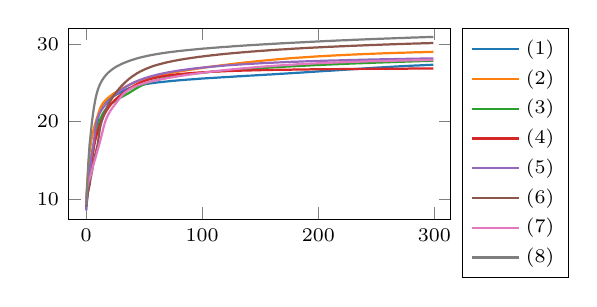
\begin{tikzpicture}

\definecolor{crimson2143940}{RGB}{214,39,40}
\definecolor{darkgray176}{RGB}{176,176,176}
\definecolor{darkorange25512714}{RGB}{255,127,14}
\definecolor{forestgreen4416044}{RGB}{44,160,44}
\definecolor{gray127}{RGB}{127,127,127}
\definecolor{mediumpurple148103189}{RGB}{148,103,189}
\definecolor{orchid227119194}{RGB}{227,119,194}
\definecolor{sienna1408675}{RGB}{140,86,75}
\definecolor{steelblue31119180}{RGB}{31,119,180}

\begin{axis}[compar, legend pos=outer north east]
\addplot [thick, steelblue31119180]
table {%
0 8.60000038146973
1 10.2700004577637
2 11.4200000762939
3 13.0299997329712
4 13.8900003433228
5 15.3999996185303
6 16.1200008392334
7 17.3600006103516
8 18.1200008392334
9 19.1800003051758
10 20.1299991607666
11 20.9400005340576
12 21.4799995422363
13 21.8500003814697
14 22.1200008392334
15 22.3299999237061
16 22.5
17 22.6499996185303
18 22.7700004577637
19 22.8799991607666
20 22.9799995422363
21 23.0699996948242
26 23.4699993133545
27 23.5400009155273
29 23.7000007629395
30 23.7700004577637
33 24.0100002288818
36 24.2199993133545
38 24.3400001525879
41 24.4899997711182
44 24.6100006103516
45 24.6399993896484
46 24.6800003051758
48 24.7399997711182
49 24.7600002288818
51 24.8199996948242
53 24.8600006103516
54 24.8899993896484
62 25.0499992370605
63 25.0599994659424
65 25.1000003814697
66 25.1100006103516
67 25.1299991607666
68 25.1399993896484
69 25.1599998474121
70 25.1700000762939
71 25.1900005340576
72 25.2000007629395
73 25.2199993133545
74 25.2299995422363
75 25.25
77 25.2700004577637
78 25.2900009155273
81 25.3199996948242
82 25.3400001525879
86 25.3799991607666
87 25.3999996185303
96 25.4899997711182
97 25.5100002288818
108 25.6200008392334
109 25.6200008392334
122 25.75
123 25.75
132 25.8400001525879
133 25.8400001525879
141 25.9200000762939
142 25.9200000762939
149 25.9899997711182
150 25.9899997711182
158 26.0699996948242
159 26.0699996948242
168 26.1599998474121
169 26.1599998474121
181 26.2800006866455
182 26.2800006866455
208 26.5400009155273
209 26.5400009155273
251 26.9599990844727
252 26.9599990844727
260 27.0400009155273
261 27.0400009155273
267 27.1000003814697
268 27.1000003814697
272 27.1399993896484
273 27.1399993896484
276 27.1700000762939
277 27.1700000762939
280 27.2000007629395
281 27.2000007629395
283 27.2199993133545
284 27.2199993133545
286 27.2399997711182
287 27.2399997711182
289 27.2600002288818
290 27.2600002288818
292 27.2800006866455
293 27.2800006866455
295 27.2999992370605
296 27.2999992370605
297 27.3099994659424
298 27.3099994659424
299 27.3199996948242
};
\addlegendentry{\scriptsize{$(1)$}}
\addplot [thick, darkorange25512714]
table {%
0 9.44999980926514
1 12.2700004577637
2 14.0500001907349
3 15.9799995422363
4 17.0699996948242
5 17.9899997711182
6 18.7000007629395
7 19.2800006866455
8 19.7900009155273
9 20.2800006866455
11 21.2199993133545
12 21.6299991607666
13 21.9699993133545
14 22.2399997711182
15 22.4500007629395
16 22.6299991607666
17 22.7900009155273
18 22.9300003051758
19 23.0599994659424
21 23.2999992370605
23 23.5200004577637
25 23.7199993133545
30 24.1700000762939
34 24.4899997711182
36 24.6299991607666
37 24.7099990844727
38 24.7800006866455
39 24.8400001525879
40 24.9099998474121
41 24.9699993133545
42 25.0400009155273
44 25.1599998474121
45 25.2099990844727
46 25.2700004577637
51 25.5200004577637
52 25.5599994659424
53 25.6100006103516
57 25.7700004577637
58 25.7999992370605
59 25.8400001525879
60 25.8700008392334
61 25.9099998474121
64 26
65 26.0400009155273
67 26.1000003814697
68 26.1200008392334
72 26.2399997711182
73 26.2600002288818
75 26.3199996948242
76 26.3400001525879
77 26.3700008392334
78 26.3899993896484
80 26.4500007629395
81 26.4699993133545
82 26.5
84 26.5400009155273
85 26.5699996948242
86 26.5900001525879
87 26.6200008392334
89 26.6599998474121
90 26.6900005340576
92 26.7299995422363
93 26.7600002288818
95 26.7999992370605
96 26.8299999237061
101 26.9300003051758
102 26.9599990844727
119 27.2999992370605
120 27.3099994659424
125 27.4099998474121
126 27.4200000762939
129 27.4799995422363
130 27.4899997711182
133 27.5499992370605
134 27.5599994659424
136 27.6000003814697
137 27.6100006103516
139 27.6499996185303
140 27.6599998474121
141 27.6800003051758
142 27.6900005340576
144 27.7299995422363
145 27.7399997711182
146 27.7600002288818
147 27.7700004577637
148 27.7900009155273
149 27.7999992370605
150 27.8199996948242
151 27.8299999237061
152 27.8500003814697
153 27.8600006103516
154 27.8799991607666
155 27.8899993896484
156 27.9099998474121
158 27.9300003051758
159 27.9500007629395
160 27.9599990844727
161 27.9799995422363
163 28
164 28.0200004577637
167 28.0499992370605
168 28.0699996948242
171 28.1000003814697
172 28.1200008392334
176 28.1599998474121
177 28.1800003051758
202 28.4300003051758
203 28.4300003051758
209 28.4899997711182
210 28.4899997711182
213 28.5200004577637
214 28.5200004577637
218 28.5599994659424
219 28.5599994659424
221 28.5799999237061
222 28.5799999237061
225 28.6100006103516
226 28.6100006103516
228 28.6299991607666
229 28.6299991607666
231 28.6499996185303
232 28.6499996185303
234 28.6700000762939
235 28.6700000762939
237 28.6900005340576
238 28.6900005340576
239 28.7000007629395
240 28.7000007629395
242 28.7199993133545
243 28.7199993133545
244 28.7299995422363
245 28.7299995422363
247 28.75
248 28.75
249 28.7600002288818
250 28.7600002288818
251 28.7700004577637
252 28.7700004577637
253 28.7800006866455
254 28.7800006866455
256 28.7999992370605
257 28.7999992370605
258 28.8099994659424
259 28.8099994659424
260 28.8199996948242
261 28.8199996948242
262 28.8299999237061
263 28.8299999237061
264 28.8400001525879
265 28.8400001525879
266 28.8500003814697
267 28.8500003814697
268 28.8600006103516
269 28.8600006103516
270 28.8700008392334
271 28.8700008392334
272 28.8799991607666
274 28.8799991607666
275 28.8899993896484
276 28.8899993896484
277 28.8999996185303
278 28.8999996185303
279 28.9099998474121
280 28.9099998474121
281 28.9200000762939
282 28.9200000762939
283 28.9300003051758
285 28.9300003051758
286 28.9400005340576
287 28.9400005340576
288 28.9500007629395
290 28.9500007629395
291 28.9599990844727
292 28.9599990844727
293 28.9699993133545
295 28.9699993133545
296 28.9799995422363
297 28.9799995422363
298 28.9899997711182
299 28.9899997711182
};
\addlegendentry{\scriptsize{$(2)$}}
\addplot [thick, forestgreen4416044]
table {%
0 9.02999973297119
1 10.9499998092651
2 12.0699996948242
3 13.0100002288818
4 14.5299997329712
5 15.7600002288818
6 16.7700004577637
7 17.2199993133545
8 17.9200000762939
9 18.3600006103516
10 19.3099994659424
11 19.7099990844727
12 20.2600002288818
13 20.5499992370605
14 20.8999996185303
15 21.1299991607666
16 21.3799991607666
17 21.5599994659424
18 21.75
19 21.9099998474121
20 22.0599994659424
21 22.2000007629395
23 22.4400005340576
24 22.5499992370605
27 22.8500003814697
28 22.9400005340576
29 23.0200004577637
30 23.1100006103516
33 23.3500003814697
34 23.4400005340576
36 23.6000003814697
38 23.7800006866455
39 23.8799991607666
41 24.0599994659424
42 24.1599998474121
43 24.25
44 24.3299999237061
45 24.4200000762939
47 24.5799999237061
51 24.8600006103516
54 25.0400009155273
58 25.2399997711182
60 25.3199996948242
61 25.3700008392334
62 25.3999996185303
64 25.4799995422363
65 25.5100002288818
66 25.5499992370605
73 25.7600002288818
74 25.7800006866455
75 25.8099994659424
76 25.8299999237061
77 25.8600006103516
79 25.8999996185303
80 25.9300003051758
90 26.1299991607666
91 26.1399993896484
94 26.2000007629395
95 26.2099990844727
97 26.25
98 26.2600002288818
99 26.2800006866455
100 26.2900009155273
101 26.3099994659424
102 26.3199996948242
103 26.3400001525879
104 26.3500003814697
105 26.3700008392334
106 26.3799991607666
107 26.3999996185303
109 26.4200000762939
110 26.4400005340576
112 26.4599990844727
113 26.4799995422363
116 26.5100002288818
117 26.5300006866455
120 26.5599994659424
121 26.5799999237061
125 26.6200008392334
126 26.6399993896484
136 26.7399997711182
137 26.7600002288818
148 26.8700008392334
149 26.8700008392334
160 26.9799995422363
161 26.9799995422363
167 27.0400009155273
168 27.0400009155273
173 27.0900001525879
174 27.0900001525879
178 27.1299991607666
179 27.1299991607666
183 27.1700000762939
184 27.1700000762939
187 27.2000007629395
188 27.2000007629395
190 27.2199993133545
191 27.2199993133545
194 27.25
195 27.25
198 27.2800006866455
199 27.2800006866455
201 27.2999992370605
202 27.2999992370605
204 27.3199996948242
205 27.3199996948242
207 27.3400001525879
208 27.3400001525879
210 27.3600006103516
211 27.3600006103516
213 27.3799991607666
214 27.3799991607666
216 27.3999996185303
217 27.3999996185303
219 27.4200000762939
220 27.4200000762939
221 27.4300003051758
222 27.4300003051758
224 27.4500007629395
225 27.4500007629395
227 27.4699993133545
228 27.4699993133545
229 27.4799995422363
230 27.4799995422363
232 27.5
233 27.5
234 27.5100002288818
235 27.5100002288818
236 27.5200004577637
237 27.5200004577637
239 27.5400009155273
240 27.5400009155273
241 27.5499992370605
242 27.5499992370605
243 27.5599994659424
244 27.5599994659424
246 27.5799999237061
247 27.5799999237061
248 27.5900001525879
249 27.5900001525879
250 27.6000003814697
251 27.6000003814697
252 27.6100006103516
253 27.6100006103516
254 27.6200008392334
255 27.6200008392334
257 27.6399993896484
258 27.6399993896484
259 27.6499996185303
260 27.6499996185303
261 27.6599998474121
262 27.6599998474121
263 27.6700000762939
264 27.6700000762939
265 27.6800003051758
266 27.6800003051758
267 27.6900005340576
268 27.6900005340576
269 27.7000007629395
270 27.7000007629395
271 27.7099990844727
272 27.7099990844727
273 27.7199993133545
274 27.7199993133545
275 27.7299995422363
276 27.7299995422363
277 27.7399997711182
278 27.7399997711182
279 27.75
280 27.75
281 27.7600002288818
282 27.7600002288818
283 27.7700004577637
285 27.7700004577637
286 27.7800006866455
287 27.7800006866455
288 27.7900009155273
289 27.7900009155273
290 27.7999992370605
291 27.7999992370605
292 27.8099994659424
293 27.8099994659424
294 27.8199996948242
296 27.8199996948242
297 27.8299999237061
298 27.8299999237061
299 27.8400001525879
};
\addlegendentry{\scriptsize{$(3)$}}
\addplot [thick, crimson2143940]
table {%
0 9.06999969482422
1 10.2600002288818
2 11.5900001525879
3 12.8900003433228
4 14.0600004196167
5 14.9799995422363
6 15.9899997711182
7 16.9200000762939
8 17.6499996185303
9 18.2299995422363
10 18.75
11 19.2099990844727
12 19.6200008392334
13 20
14 20.3600006103516
15 20.6800003051758
16 20.9799995422363
17 21.25
18 21.5100002288818
20 21.9500007629395
22 22.3299999237061
24 22.6499996185303
25 22.7900009155273
26 22.9400005340576
28 23.2000007629395
29 23.3099994659424
30 23.4400005340576
35 23.9899997711182
40 24.4899997711182
41 24.5799999237061
42 24.6599998474121
43 24.75
44 24.8199996948242
45 24.8999996185303
47 25.0400009155273
50 25.2199993133545
54 25.4200000762939
59 25.6200008392334
62 25.7099990844727
63 25.75
64 25.7700004577637
66 25.8299999237061
67 25.8500003814697
68 25.8799991607666
70 25.9200000762939
71 25.9500007629395
75 26.0300006866455
76 26.0400009155273
79 26.1000003814697
80 26.1100006103516
81 26.1299991607666
82 26.1399993896484
83 26.1599998474121
85 26.1800003051758
86 26.2000007629395
89 26.2299995422363
90 26.25
102 26.3700008392334
103 26.3700008392334
107 26.4099998474121
108 26.4099998474121
111 26.4400005340576
112 26.4400005340576
114 26.4599990844727
115 26.4599990844727
116 26.4699993133545
117 26.4699993133545
119 26.4899997711182
120 26.4899997711182
121 26.5
122 26.5
123 26.5100002288818
124 26.5100002288818
125 26.5200004577637
126 26.5200004577637
127 26.5300006866455
128 26.5300006866455
129 26.5400009155273
130 26.5400009155273
131 26.5499992370605
132 26.5499992370605
133 26.5599994659424
134 26.5599994659424
135 26.5699996948242
136 26.5699996948242
137 26.5799999237061
139 26.5799999237061
140 26.5900001525879
142 26.5900001525879
143 26.6000003814697
144 26.6000003814697
145 26.6100006103516
147 26.6100006103516
148 26.6200008392334
150 26.6200008392334
151 26.6299991607666
153 26.6299991607666
154 26.6399993896484
157 26.6399993896484
158 26.6499996185303
160 26.6499996185303
161 26.6599998474121
164 26.6599998474121
165 26.6700000762939
168 26.6700000762939
169 26.6800003051758
172 26.6800003051758
173 26.6900005340576
177 26.6900005340576
178 26.7000007629395
181 26.7000007629395
182 26.7099990844727
186 26.7099990844727
187 26.7199993133545
192 26.7199993133545
193 26.7299995422363
198 26.7299995422363
199 26.7399997711182
204 26.7399997711182
205 26.75
211 26.75
212 26.7600002288818
218 26.7600002288818
219 26.7700004577637
226 26.7700004577637
227 26.7800006866455
234 26.7800006866455
235 26.7900009155273
244 26.7900009155273
245 26.7999992370605
254 26.7999992370605
255 26.8099994659424
265 26.8099994659424
266 26.8199996948242
277 26.8199996948242
278 26.8299999237061
290 26.8299999237061
291 26.8400001525879
299 26.8400001525879
};
\addlegendentry{\scriptsize{$(4)$}}
\addplot [thick, mediumpurple148103189]
table {%
0 8.5
2 11.8900003433228
3 13.5
4 14.6099996566772
5 15.9399995803833
6 16.6800003051758
7 17.7999992370605
8 19.0499992370605
9 19.9599990844727
10 20.4599990844727
11 20.8400001525879
12 21.1399993896484
13 21.3999996185303
14 21.6299991607666
15 21.8400001525879
16 22.0300006866455
18 22.3899993896484
21 22.8700008392334
24 23.2900009155273
25 23.4200000762939
26 23.5400009155273
27 23.6700000762939
28 23.7900009155273
29 23.8999996185303
30 24.0200004577637
32 24.2399997711182
35 24.5400009155273
36 24.6299991607666
40 24.9500007629395
42 25.0900001525879
43 25.1499996185303
44 25.2199993133545
47 25.3999996185303
49 25.5
50 25.5599994659424
51 25.6100006103516
52 25.6499996185303
54 25.75
61 26.0300006866455
62 26.0599994659424
63 26.1000003814697
65 26.1599998474121
66 26.2000007629395
71 26.3500003814697
72 26.3700008392334
74 26.4300003051758
75 26.4500007629395
76 26.4799995422363
77 26.5
78 26.5300006866455
80 26.5699996948242
81 26.6000003814697
93 26.8400001525879
94 26.8500003814697
97 26.9099998474121
98 26.9200000762939
99 26.9400005340576
100 26.9500007629395
102 26.9899997711182
103 27
104 27.0200004577637
106 27.0400009155273
107 27.0599994659424
108 27.0699996948242
109 27.0900001525879
111 27.1100006103516
112 27.1299991607666
114 27.1499996185303
115 27.1700000762939
119 27.2099990844727
120 27.2299995422363
143 27.4599990844727
144 27.4599990844727
148 27.5
149 27.5
153 27.5400009155273
154 27.5400009155273
157 27.5699996948242
158 27.5699996948242
160 27.5900001525879
161 27.5900001525879
163 27.6100006103516
164 27.6100006103516
166 27.6299991607666
167 27.6299991607666
169 27.6499996185303
170 27.6499996185303
172 27.6700000762939
173 27.6700000762939
174 27.6800003051758
175 27.6800003051758
177 27.7000007629395
178 27.7000007629395
179 27.7099990844727
180 27.7099990844727
181 27.7199993133545
182 27.7199993133545
184 27.7399997711182
185 27.7399997711182
186 27.75
187 27.75
188 27.7600002288818
189 27.7600002288818
190 27.7700004577637
191 27.7700004577637
192 27.7800006866455
193 27.7800006866455
194 27.7900009155273
195 27.7900009155273
196 27.7999992370605
197 27.7999992370605
198 27.8099994659424
199 27.8099994659424
200 27.8199996948242
201 27.8199996948242
202 27.8299999237061
204 27.8299999237061
205 27.8400001525879
206 27.8400001525879
207 27.8500003814697
208 27.8500003814697
209 27.8600006103516
211 27.8600006103516
212 27.8700008392334
213 27.8700008392334
214 27.8799991607666
215 27.8799991607666
216 27.8899993896484
218 27.8899993896484
219 27.8999996185303
220 27.8999996185303
221 27.9099998474121
223 27.9099998474121
224 27.9200000762939
225 27.9200000762939
226 27.9300003051758
228 27.9300003051758
229 27.9400005340576
231 27.9400005340576
232 27.9500007629395
234 27.9500007629395
235 27.9599990844727
236 27.9599990844727
237 27.9699993133545
239 27.9699993133545
240 27.9799995422363
242 27.9799995422363
243 27.9899997711182
245 27.9899997711182
246 28
248 28
249 28.0100002288818
252 28.0100002288818
253 28.0200004577637
255 28.0200004577637
256 28.0300006866455
258 28.0300006866455
259 28.0400009155273
261 28.0400009155273
262 28.0499992370605
265 28.0499992370605
266 28.0599994659424
268 28.0599994659424
269 28.0699996948242
272 28.0699996948242
273 28.0799999237061
275 28.0799999237061
276 28.0900001525879
279 28.0900001525879
280 28.1000003814697
283 28.1000003814697
284 28.1100006103516
287 28.1100006103516
288 28.1200008392334
291 28.1200008392334
292 28.1299991607666
294 28.1299991607666
295 28.1399993896484
299 28.1399993896484
};
\addlegendentry{\scriptsize{$(5)$}}
\addplot [thick, sienna1408675]
table {%
0 9.0600004196167
1 10.4300003051758
3 11.7799997329712
4 12.7700004577637
5 13.4399995803833
6 14.3599996566772
7 15.1800003051758
8 15.7799997329712
10 17.0499992370605
11 18.1299991607666
12 19.1700000762939
13 19.7900009155273
14 20.2900009155273
15 20.75
16 21.1499996185303
17 21.5
18 21.8299999237061
19 22.1200008392334
20 22.3999996185303
21 22.6599998474121
22 22.9099998474121
23 23.1499996185303
24 23.3700008392334
25 23.5799999237061
26 23.7800006866455
28 24.1599998474121
30 24.5
31 24.6599998474121
33 24.9599990844727
35 25.2399997711182
37 25.5
38 25.6100006103516
39 25.7299995422363
40 25.8400001525879
43 26.1399993896484
44 26.2299995422363
45 26.3099994659424
46 26.3999996185303
47 26.4799995422363
51 26.7600002288818
55 27
56 27.0499992370605
57 27.1100006103516
59 27.2099990844727
60 27.25
61 27.2999992370605
68 27.5799999237061
69 27.6100006103516
70 27.6499996185303
73 27.7399997711182
74 27.7800006866455
76 27.8400001525879
77 27.8600006103516
80 27.9500007629395
81 27.9699993133545
82 28
83 28.0200004577637
84 28.0499992370605
85 28.0699996948242
86 28.1000003814697
88 28.1399993896484
89 28.1700000762939
94 28.2700004577637
95 28.2999992370605
98 28.3600006103516
99 28.3700008392334
104 28.4699993133545
105 28.4799995422363
108 28.5400009155273
109 28.5499992370605
111 28.5900001525879
112 28.6000003814697
114 28.6399993896484
115 28.6499996185303
116 28.6700000762939
117 28.6800003051758
118 28.7000007629395
119 28.7099990844727
120 28.7299995422363
121 28.7399997711182
122 28.7600002288818
124 28.7800006866455
125 28.7999992370605
126 28.8099994659424
127 28.8299999237061
129 28.8500003814697
130 28.8700008392334
132 28.8899993896484
133 28.9099998474121
136 28.9400005340576
137 28.9599990844727
140 28.9899997711182
141 29.0100002288818
146 29.0599994659424
147 29.0799999237061
156 29.1700000762939
157 29.1900005340576
169 29.3099994659424
170 29.3099994659424
180 29.4099998474121
181 29.4099998474121
187 29.4699993133545
188 29.4699993133545
192 29.5100002288818
193 29.5100002288818
197 29.5499992370605
198 29.5499992370605
201 29.5799999237061
202 29.5799999237061
205 29.6100006103516
206 29.6100006103516
209 29.6399993896484
210 29.6399993896484
212 29.6599998474121
213 29.6599998474121
215 29.6800003051758
216 29.6800003051758
218 29.7000007629395
219 29.7000007629395
221 29.7199993133545
222 29.7199993133545
224 29.7399997711182
225 29.7399997711182
227 29.7600002288818
228 29.7600002288818
230 29.7800006866455
231 29.7800006866455
232 29.7900009155273
233 29.7900009155273
235 29.8099994659424
236 29.8099994659424
237 29.8199996948242
238 29.8199996948242
240 29.8400001525879
241 29.8400001525879
242 29.8500003814697
243 29.8500003814697
245 29.8700008392334
246 29.8700008392334
247 29.8799991607666
248 29.8799991607666
249 29.8899993896484
250 29.8899993896484
251 29.8999996185303
252 29.8999996185303
254 29.9200000762939
255 29.9200000762939
256 29.9300003051758
257 29.9300003051758
258 29.9400005340576
259 29.9400005340576
260 29.9500007629395
261 29.9500007629395
262 29.9599990844727
263 29.9599990844727
264 29.9699993133545
265 29.9699993133545
266 29.9799995422363
267 29.9799995422363
268 29.9899997711182
269 29.9899997711182
270 30
271 30
272 30.0100002288818
273 30.0100002288818
274 30.0200004577637
275 30.0200004577637
276 30.0300006866455
277 30.0300006866455
278 30.0400009155273
279 30.0400009155273
280 30.0499992370605
281 30.0499992370605
282 30.0599994659424
283 30.0599994659424
284 30.0699996948242
286 30.0699996948242
287 30.0799999237061
288 30.0799999237061
289 30.0900001525879
290 30.0900001525879
291 30.1000003814697
292 30.1000003814697
293 30.1100006103516
295 30.1100006103516
296 30.1200008392334
297 30.1200008392334
298 30.1299991607666
299 30.1299991607666
};
\addlegendentry{\scriptsize{$(6)$}}
\addplot [thick, orchid227119194]
table {%
0 9.61999988555908
1 11.5
2 12.1599998474121
3 12.6300001144409
4 13.039999961853
5 13.6800003051758
6 14.2799997329712
7 14.7799997329712
8 15.2600002288818
11 16.8600006103516
12 17.4099998474121
13 17.9799995422363
14 18.5900001525879
15 19.2199993133545
16 19.7600002288818
17 20.2000007629395
18 20.5599994659424
19 20.8700008392334
20 21.1399993896484
21 21.3899993896484
23 21.8299999237061
26 22.4300003051758
29 23
31 23.3600006103516
33 23.6599998474121
34 23.7900009155273
36 24.0100002288818
37 24.1100006103516
38 24.2000007629395
40 24.3600006103516
42 24.5
45 24.6800003051758
49 24.8799991607666
50 24.9200000762939
51 24.9699993133545
55 25.1299991607666
56 25.1599998474121
57 25.2000007629395
58 25.2299995422363
59 25.2700004577637
61 25.3299999237061
62 25.3700008392334
67 25.5200004577637
68 25.5400009155273
71 25.6299991607666
72 25.6499996185303
74 25.7099990844727
75 25.7299995422363
76 25.7600002288818
77 25.7800006866455
78 25.8099994659424
79 25.8299999237061
80 25.8600006103516
82 25.8999996185303
83 25.9300003051758
86 25.9899997711182
87 26.0200004577637
94 26.1599998474121
95 26.1900005340576
97 26.2299995422363
98 26.2399997711182
106 26.3999996185303
107 26.4099998474121
110 26.4699993133545
111 26.4799995422363
114 26.5400009155273
115 26.5499992370605
117 26.5900001525879
118 26.6000003814697
119 26.6200008392334
120 26.6299991607666
122 26.6700000762939
123 26.6800003051758
124 26.7000007629395
125 26.7099990844727
126 26.7299995422363
127 26.7399997711182
128 26.7600002288818
129 26.7700004577637
130 26.7900009155273
132 26.8099994659424
133 26.8299999237061
134 26.8400001525879
135 26.8600006103516
137 26.8799991607666
138 26.8999996185303
140 26.9200000762939
141 26.9400005340576
143 26.9599990844727
144 26.9799995422363
147 27.0100002288818
148 27.0300006866455
152 27.0699996948242
153 27.0900001525879
160 27.1599998474121
161 27.1800003051758
175 27.3199996948242
176 27.3199996948242
184 27.3999996185303
185 27.3999996185303
189 27.4400005340576
190 27.4400005340576
194 27.4799995422363
195 27.4799995422363
197 27.5
198 27.5
201 27.5300006866455
202 27.5300006866455
204 27.5499992370605
205 27.5499992370605
207 27.5699996948242
208 27.5699996948242
210 27.5900001525879
211 27.5900001525879
213 27.6100006103516
214 27.6100006103516
215 27.6200008392334
216 27.6200008392334
218 27.6399993896484
219 27.6399993896484
220 27.6499996185303
221 27.6499996185303
222 27.6599998474121
223 27.6599998474121
224 27.6700000762939
225 27.6700000762939
226 27.6800003051758
227 27.6800003051758
229 27.7000007629395
230 27.7000007629395
231 27.7099990844727
232 27.7099990844727
233 27.7199993133545
235 27.7199993133545
236 27.7299995422363
237 27.7299995422363
238 27.7399997711182
239 27.7399997711182
240 27.75
241 27.75
242 27.7600002288818
243 27.7600002288818
244 27.7700004577637
246 27.7700004577637
247 27.7800006866455
248 27.7800006866455
249 27.7900009155273
251 27.7900009155273
252 27.7999992370605
253 27.7999992370605
254 27.8099994659424
256 27.8099994659424
257 27.8199996948242
259 27.8199996948242
260 27.8299999237061
262 27.8299999237061
263 27.8400001525879
264 27.8400001525879
265 27.8500003814697
267 27.8500003814697
268 27.8600006103516
271 27.8600006103516
272 27.8700008392334
274 27.8700008392334
275 27.8799991607666
277 27.8799991607666
278 27.8899993896484
281 27.8899993896484
282 27.8999996185303
285 27.8999996185303
286 27.9099998474121
289 27.9099998474121
290 27.9200000762939
293 27.9200000762939
294 27.9300003051758
297 27.9300003051758
298 27.9400005340576
299 27.9400005340576
};
\addlegendentry{\scriptsize{$(7)$}}
\addplot [thick, gray127]
table {%
0 9.1899995803833
1 11.8400001525879
2 14.8599996566772
3 17.0200004577637
4 18.4300003051758
5 19.8999996185303
6 21.0400009155273
7 22.0300006866455
8 22.8500003814697
9 23.5200004577637
10 24.0400009155273
11 24.4599990844727
12 24.8099994659424
13 25.1100006103516
14 25.3600006103516
15 25.5900001525879
16 25.7900009155273
17 25.9699993133545
18 26.1399993896484
19 26.2900009155273
20 26.4300003051758
22 26.6700000762939
23 26.7800006866455
25 26.9799995422363
26 27.0699996948242
29 27.3099994659424
32 27.5200004577637
36 27.7600002288818
37 27.8099994659424
38 27.8700008392334
40 27.9699993133545
41 28.0100002288818
42 28.0599994659424
43 28.1000003814697
44 28.1499996185303
48 28.3099994659424
49 28.3400001525879
50 28.3799991607666
52 28.4400005340576
53 28.4799995422363
57 28.6000003814697
58 28.6200008392334
60 28.6800003051758
61 28.7000007629395
62 28.7299995422363
63 28.75
64 28.7800006866455
67 28.8400001525879
68 28.8700008392334
75 29.0100002288818
76 29.0200004577637
79 29.0799999237061
80 29.0900001525879
82 29.1299991607666
83 29.1399993896484
85 29.1800003051758
86 29.1900005340576
87 29.2099990844727
88 29.2199993133545
89 29.2399997711182
90 29.25
91 29.2700004577637
92 29.2800006866455
93 29.2999992370605
95 29.3199996948242
96 29.3400001525879
97 29.3500003814697
98 29.3700008392334
100 29.3899993896484
101 29.4099998474121
104 29.4400005340576
105 29.4599990844727
108 29.4899997711182
109 29.5100002288818
114 29.5599994659424
115 29.5799999237061
124 29.6700000762939
125 29.6900005340576
143 29.8700008392334
144 29.8700008392334
154 29.9699993133545
155 29.9699993133545
162 30.0400009155273
163 30.0400009155273
168 30.0900001525879
169 30.0900001525879
174 30.1399993896484
175 30.1399993896484
178 30.1700000762939
179 30.1700000762939
183 30.2099990844727
184 30.2099990844727
187 30.2399997711182
188 30.2399997711182
191 30.2700004577637
192 30.2700004577637
195 30.2999992370605
196 30.2999992370605
199 30.3299999237061
200 30.3299999237061
202 30.3500003814697
203 30.3500003814697
206 30.3799991607666
207 30.3799991607666
209 30.3999996185303
210 30.3999996185303
212 30.4200000762939
213 30.4200000762939
216 30.4500007629395
217 30.4500007629395
219 30.4699993133545
220 30.4699993133545
222 30.4899997711182
223 30.4899997711182
224 30.5
225 30.5
227 30.5200004577637
228 30.5200004577637
230 30.5400009155273
231 30.5400009155273
233 30.5599994659424
234 30.5599994659424
236 30.5799999237061
237 30.5799999237061
238 30.5900001525879
239 30.5900001525879
241 30.6100006103516
242 30.6100006103516
243 30.6200008392334
244 30.6200008392334
246 30.6399993896484
247 30.6399993896484
248 30.6499996185303
249 30.6499996185303
251 30.6700000762939
252 30.6700000762939
253 30.6800003051758
254 30.6800003051758
255 30.6900005340576
256 30.6900005340576
258 30.7099990844727
259 30.7099990844727
260 30.7199993133545
261 30.7199993133545
262 30.7299995422363
263 30.7299995422363
265 30.75
266 30.75
267 30.7600002288818
268 30.7600002288818
269 30.7700004577637
270 30.7700004577637
271 30.7800006866455
272 30.7800006866455
273 30.7900009155273
274 30.7900009155273
275 30.7999992370605
276 30.7999992370605
278 30.8199996948242
279 30.8199996948242
280 30.8299999237061
281 30.8299999237061
282 30.8400001525879
283 30.8400001525879
284 30.8500003814697
285 30.8500003814697
286 30.8600006103516
287 30.8600006103516
288 30.8700008392334
289 30.8700008392334
290 30.8799991607666
291 30.8799991607666
292 30.8899993896484
293 30.8899993896484
294 30.8999996185303
295 30.8999996185303
296 30.9099998474121
297 30.9099998474121
298 30.9200000762939
299 30.9200000762939
};
\addlegendentry{\scriptsize{$(8)$}}
\end{axis}

\end{tikzpicture}
}
\end{tabular}
	\caption{Plein de descentes ---  avec passe-bas gaussien ($\sigma=0.6$)}
	\label{fig:LGDunif-g}
\end{figure}
\begin{figure}[H]\centering
	\begin{tabular}{c c c c c c c c c}
$(1)$  &  $(2)$  &  $(3)$  &  $(4)$  &  $(5)$  &  $(6)$  &  $(7)$  &  $(8)$

\\

\includegraphics[width=0.1\textwidth]{resultats/PGD/multitarget/rand_gauss_1-init-pas=1.25_filtre=s-None}
&
\includegraphics[width=0.1\textwidth]{resultats/PGD/multitarget/rand_gauss_2-init-pas=1.25_filtre=s-None}
&
\includegraphics[width=0.1\textwidth]{resultats/PGD/multitarget/rand_gauss_3-init-pas=1.25_filtre=s-None}
&
\includegraphics[width=0.1\textwidth]{resultats/PGD/multitarget/rand_gauss_4-init-pas=1.25_filtre=s-None}
&
\includegraphics[width=0.1\textwidth]{resultats/PGD/multitarget/rand_gauss_5-init-pas=1.25_filtre=s-None}
&
\includegraphics[width=0.1\textwidth]{resultats/PGD/multitarget/rand_gauss_6-init-pas=1.25_filtre=s-None}
&
\includegraphics[width=0.1\textwidth]{resultats/PGD/multitarget/rand_gauss_7-init-pas=1.25_filtre=s-None}
&
\includegraphics[width=0.1\textwidth]{resultats/PGD/multitarget/rand_gauss_8-init-pas=1.25_filtre=s-None}

\\

\includegraphics[width=0.1\textwidth]{resultats/PGD/multitarget/rand_gauss_1-guess-pas=1.25_filtre=s-None.png}
&
\includegraphics[width=0.1\textwidth]{resultats/PGD/multitarget/rand_gauss_2-guess-pas=1.25_filtre=s-None}
&
\includegraphics[width=0.1\textwidth]{resultats/PGD/multitarget/rand_gauss_3-guess-pas=1.25_filtre=s-None}
&
\includegraphics[width=0.1\textwidth]{resultats/PGD/multitarget/rand_gauss_4-guess-pas=1.25_filtre=s-None}
&
\includegraphics[width=0.1\textwidth]{resultats/PGD/multitarget/rand_gauss_5-guess-pas=1.25_filtre=s-None}
&
\includegraphics[width=0.1\textwidth]{resultats/PGD/multitarget/rand_gauss_6-guess-pas=1.25_filtre=s-None}
&
\includegraphics[width=0.1\textwidth]{resultats/PGD/multitarget/rand_gauss_7-guess-pas=1.25_filtre=s-None}
&
\includegraphics[width=0.1\textwidth]{resultats/PGD/multitarget/rand_gauss_8-guess-pas=1.25_filtre=s-None}

\\

\includegraphics[width=0.1\textwidth]{resultats/PGD/multitarget/rand_gauss_1-target-pas=1.25_filtre=s-None}
&
\includegraphics[width=0.1\textwidth]{resultats/PGD/multitarget/rand_gauss_2-target-pas=1.25_filtre=s-None}
&
\includegraphics[width=0.1\textwidth]{resultats/PGD/multitarget/rand_gauss_3-target-pas=1.25_filtre=s-None}
&
\includegraphics[width=0.1\textwidth]{resultats/PGD/multitarget/rand_gauss_4-target-pas=1.25_filtre=s-None}
&
\includegraphics[width=0.1\textwidth]{resultats/PGD/multitarget/rand_gauss_5-target-pas=1.25_filtre=s-None}
&
\includegraphics[width=0.1\textwidth]{resultats/PGD/multitarget/rand_gauss_6-target-pas=1.25_filtre=s-None}
&
\includegraphics[width=0.1\textwidth]{resultats/PGD/multitarget/rand_gauss_7-target-pas=1.25_filtre=s-None}
&
\includegraphics[width=0.1\textwidth]{resultats/PGD/multitarget/rand_gauss_8-target-pas=1.25_filtre=s-None}

\\ \\



\multicolumn{4}{c}{Loss}  &  \multicolumn{5}{c}{PSNR{\color{white}bbbb}}

\\

\multicolumn{4}{c}{% This file was created with tikzplotlib v0.10.1.
\begin{tikzpicture}

\definecolor{crimson2143940}{RGB}{214,39,40}
\definecolor{darkgray176}{RGB}{176,176,176}
\definecolor{darkorange25512714}{RGB}{255,127,14}
\definecolor{forestgreen4416044}{RGB}{44,160,44}
\definecolor{gray127}{RGB}{127,127,127}
\definecolor{mediumpurple148103189}{RGB}{148,103,189}
\definecolor{orchid227119194}{RGB}{227,119,194}
\definecolor{sienna1408675}{RGB}{140,86,75}
\definecolor{steelblue31119180}{RGB}{31,119,180}

\begin{axis}[
height=\figheight,
tick align=outside,
tick pos=left,
width=\figwidth,
x grid style={darkgray176},
xmin=-1.2, xmax=25.2,
xtick style={color=black},
y grid style={darkgray176},
ymin=-0.938261824846268, ymax=32.3032843649387,
ytick style={color=black}
]
\addplot [semithick, steelblue31119180]
table {%
0 27.61279296875
1 5.0438117980957
2 3.59597158432007
3 2.72845482826233
4 1.81588268280029
5 1.23482871055603
6 0.977622985839844
7 0.833596229553223
8 0.75908887386322
9 0.721545457839966
10 0.69955313205719
12 0.679590225219727
17 0.655109524726868
22 0.647685050964355
24 0.647486686706543
};
\addplot [semithick, darkorange25512714]
table {%
0 30.2018527984619
1 4.30142021179199
2 3.06181502342224
3 2.24562692642212
4 1.73758697509766
5 1.33212351799011
6 1.06765758991241
7 0.962657690048218
8 0.966707944869995
9 1.04626560211182
10 1.16426432132721
11 1.26813435554504
12 1.33266735076904
13 1.36687672138214
14 1.3843080997467
16 1.39778101444244
20 1.40165567398071
24 1.40103375911713
};
\addplot [semithick, forestgreen4416044]
table {%
0 26.8727149963379
1 3.62669920921326
2 2.8121862411499
3 2.36822080612183
4 1.9517012834549
5 1.5463719367981
6 1.19763290882111
7 1.02643001079559
8 0.948850631713867
9 0.883724808692932
10 0.804481387138367
11 0.70289421081543
12 0.610994219779968
13 0.572717547416687
14 0.57528018951416
16 0.616444230079651
18 0.657610177993774
20 0.685601949691772
23 0.712594747543335
24 0.719223141670227
};
\addplot [semithick, crimson2143940]
table {%
0 26.2570705413818
1 4.77597332000732
2 3.65266585350037
3 2.87369227409363
4 2.23165130615234
5 1.76792907714844
6 1.48932075500488
7 1.28381013870239
8 1.13417935371399
9 1.02215611934662
10 0.93181049823761
11 0.856253862380981
12 0.802581906318665
13 0.77596640586853
14 0.771467447280884
16 0.795935869216919
18 0.820542812347412
21 0.837147951126099
24 0.84443473815918
};
\addplot [semithick, mediumpurple148103189]
table {%
0 30.7923049926758
1 5.7014856338501
2 4.11674165725708
3 3.11512422561646
4 2.5389289855957
5 2.12082099914551
6 1.71534430980682
7 1.42888295650482
8 1.28847920894623
9 1.24013710021973
11 1.20909512042999
12 1.18352580070496
14 1.11899626255035
15 1.0945121049881
16 1.08555746078491
17 1.09675228595734
23 1.23627996444702
24 1.24865317344666
};
\addplot [semithick, sienna1408675]
table {%
0 29.1503982543945
1 4.32221984863281
2 3.14383268356323
3 2.47220396995544
4 2.06153249740601
5 1.81038641929626
6 1.75876605510712
7 1.79904055595398
8 1.86570477485657
9 1.91420090198517
10 1.94782483577728
11 1.96868252754211
12 1.97489655017853
17 1.96467113494873
24 2.00118184089661
};
\addplot [semithick, orchid227119194]
table {%
0 29.7836570739746
1 3.80904459953308
2 3.01426959037781
3 2.63571310043335
4 2.49578976631165
5 2.38946437835693
6 2.29241323471069
9 2.03860473632812
10 1.94246697425842
13 1.62619388103485
14 1.53589510917664
15 1.46184754371643
16 1.40454578399658
17 1.36919021606445
18 1.35092663764954
20 1.34143722057343
24 1.34655249118805
};
\addplot [semithick, gray127]
table {%
0 25.9946193695068
1 5.90621614456177
2 4.4400839805603
3 3.33432388305664
4 2.46125197410583
5 1.94792699813843
6 1.73100769519806
7 1.649658203125
8 1.63047862052917
9 1.63957488536835
11 1.67223465442657
12 1.68076062202454
13 1.68049716949463
19 1.6337628364563
24 1.6240828037262
};
\end{axis}

\end{tikzpicture}
}
&
\multicolumn{5}{c}{% This file was created with tikzplotlib v0.10.1.
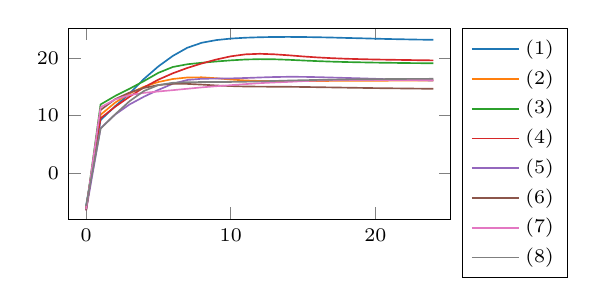
\begin{tikzpicture}

\definecolor{crimson2143940}{RGB}{214,39,40}
\definecolor{darkgray176}{RGB}{176,176,176}
\definecolor{darkorange25512714}{RGB}{255,127,14}
\definecolor{forestgreen4416044}{RGB}{44,160,44}
\definecolor{gray127}{RGB}{127,127,127}
\definecolor{mediumpurple148103189}{RGB}{148,103,189}
\definecolor{orchid227119194}{RGB}{227,119,194}
\definecolor{sienna1408675}{RGB}{140,86,75}
\definecolor{steelblue31119180}{RGB}{31,119,180}

\begin{axis}[compar, legend pos=outer north east]
\addplot [semithick, steelblue31119180]
table {%
0 -5.6399998664856
1 9.23999977111816
2 11.6199998855591
3 13.8199996948242
4 16.3600006103516
5 18.5400009155273
6 20.3500003814697
7 21.7600002288818
8 22.6200008392334
9 23.0799999237061
10 23.3400001525879
11 23.4899997711182
12 23.5699996948242
13 23.6200008392334
14 23.6299991607666
15 23.6100006103516
16 23.5699996948242
17 23.5200004577637
18 23.4500007629395
19 23.3899993896484
20 23.3199996948242
21 23.2600002288818
23 23.1599998474121
24 23.1299991607666
 };
\addlegendentry{\scriptsize{$(1)$}}
\addplot [semithick, darkorange25512714]
table {%
0 -6.28000020980835
1 10.1499996185303
2 12.25
3 13.8500003814697
4 15.0100002288818
5 15.8299999237061
6 16.3500003814697
7 16.6100006103516
8 16.6399993896484
9 16.4799995422363
10 16.2600002288818
11 16.1000003814697
12 16.0100002288818
13 15.9799995422363
14 15.9799995422363
16 16
17 16.0200004577637
22 16.0699996948242
24 16.0699996948242
 };
\addlegendentry{\scriptsize{$(2)$}}
\addplot [semithick, forestgreen4416044]
table {%
0 -6.21000003814697
1 11.9399995803833
2 13.3999996185303
3 14.6599998474121
4 15.9899997711182
5 17.4200000762939
6 18.4300003051758
7 18.8999996185303
8 19.1599998474121
9 19.3799991607666
10 19.5699996948242
11 19.7199993133545
12 19.7800006866455
13 19.7600002288818
14 19.6700000762939
15 19.5499992370605
16 19.4400005340576
17 19.3500003814697
18 19.2800006866455
20 19.1800003051758
21 19.1499996185303
22 19.1100006103516
23 19.0900001525879
24 19.0599994659424
 };
\addlegendentry{\scriptsize{$(3)$}}
\addplot [semithick, crimson2143940]
table {%
0 -6.09999990463257
1 9.55000019073486
2 11.5299997329712
3 13.2799997329712
4 14.8999996185303
5 16.2399997711182
6 17.3400001525879
7 18.2600002288818
8 19.0400009155273
9 19.7199993133545
10 20.2700004577637
11 20.6100006103516
12 20.7099990844727
13 20.6200008392334
14 20.4500007629395
15 20.25
16 20.0799999237061
17 19.9500007629395
18 19.8500003814697
19 19.7800006866455
20 19.7199993133545
23 19.6000003814697
24 19.5699996948242
 };
\addlegendentry{\scriptsize{$(4)$}}
\addplot [semithick, mediumpurple148103189]
table {%
0 -6.40000009536743
1 7.82000017166138
2 10.1800003051758
3 11.9399995803833
4 13.289999961853
5 14.4700002670288
6 15.5299997329712
7 16.1800003051758
8 16.3899993896484
10 16.4500007629395
11 16.5200004577637
12 16.6100006103516
13 16.6900005340576
14 16.7299995422363
15 16.7199993133545
16 16.6700000762939
19 16.4599990844727
20 16.3799991607666
21 16.2900009155273
22 16.2099990844727
23 16.1399993896484
24 16.0799999237061
 };
\addlegendentry{\scriptsize{$(5)$}}
\addplot [semithick, sienna1408675]
table {%
0 -6.40000009536743
1 10.9799995422363
2 12.8500003814697
3 14
4 14.8000001907349
5 15.3100004196167
6 15.5100002288818
7 15.5
8 15.3800001144409
9 15.2299995422363
10 15.1199998855591
11 15.0500001907349
13 15.0100002288818
14 15
15 14.9700002670288
20 14.7700004577637
24 14.6499996185303
 };
\addlegendentry{\scriptsize{$(6)$}}
\addplot [semithick, orchid227119194]
table {%
0 -6.15999984741211
1 11.4499998092651
2 12.8000001907349
3 13.5699996948242
4 13.9499998092651
5 14.1899995803833
6 14.4200000762939
8 14.8999996185303
9 15.1000003814697
11 15.460000038147
12 15.6300001144409
13 15.75
14 15.8500003814697
15 15.9799995422363
16 16.0699996948242
17 16.1299991607666
18 16.1700000762939
19 16.1800003051758
21 16.1800003051758
22 16.1700000762939
24 16.1700000762939
 };
\addlegendentry{\scriptsize{$(7)$}}
\addplot [semithick, gray127]
table {%
0 -5.55999994277954
1 7.76000022888184
2 10.2200002670288
3 12.5
4 14.2799997329712
5 15.3000001907349
6 15.6999998092651
7 15.8000001907349
8 15.8199996948242
9 15.8199996948242
10 15.8400001525879
11 15.8800001144409
12 15.9399995803833
14 16.0799999237061
15 16.1399993896484
16 16.1900005340576
18 16.2700004577637
19 16.2999992370605
22 16.3600006103516
24 16.3799991607666
 };
\addlegendentry{\scriptsize{$(8)$}}
\end{axis}

\end{tikzpicture}
}
\end{tabular}
    \caption{Plein de descentes --- sans passe-bas}
    \label{fig:LGDgauss-s}
\end{figure}
\begin{figure}[H]\centering
	\begin{tabular}{c c c c c c c c c}
	$(1)$  &  $(2)$  &  $(3)$  &  $(4)$  &  $(5)$  &  $(6)$  &  $(7)$  &  $(8)$
	
	\\
	
	\includegraphics[width=0.1\textwidth]{resultats/LGD/multitarget/gauss_1-init-pas=0.25_filtre=g-0.6}
	&
	\includegraphics[width=0.1\textwidth]{resultats/LGD/multitarget/gauss_2-init-pas=0.25_filtre=g-0.6}
	&
	\includegraphics[width=0.1\textwidth]{resultats/LGD/multitarget/gauss_3-init-pas=0.25_filtre=g-0.6}
	&
	\includegraphics[width=0.1\textwidth]{resultats/LGD/multitarget/gauss_4-init-pas=0.25_filtre=g-0.6}
	&
	\includegraphics[width=0.1\textwidth]{resultats/LGD/multitarget/gauss_5-init-pas=0.25_filtre=g-0.6}
	&
	\includegraphics[width=0.1\textwidth]{resultats/LGD/multitarget/gauss_6-init-pas=0.25_filtre=g-0.6}
	&
	\includegraphics[width=0.1\textwidth]{resultats/LGD/multitarget/gauss_7-init-pas=0.25_filtre=g-0.6}
	&
	\includegraphics[width=0.1\textwidth]{resultats/LGD/multitarget/gauss_8-init-pas=0.25_filtre=g-0.6}
	
	\\
	
	\includegraphics[width=0.1\textwidth]{resultats/LGD/multitarget/gauss_1-guess-pas=0.25_filtre=g-0.6}
	&
	\includegraphics[width=0.1\textwidth]{resultats/LGD/multitarget/gauss_2-guess-pas=0.25_filtre=g-0.6}
	&
	\includegraphics[width=0.1\textwidth]{resultats/LGD/multitarget/gauss_3-guess-pas=0.25_filtre=g-0.6}
	&
	\includegraphics[width=0.1\textwidth]{resultats/LGD/multitarget/gauss_4-guess-pas=0.25_filtre=g-0.6}
	&
	\includegraphics[width=0.1\textwidth]{resultats/LGD/multitarget/gauss_5-guess-pas=0.25_filtre=g-0.6}
	&
	\includegraphics[width=0.1\textwidth]{resultats/LGD/multitarget/gauss_6-guess-pas=0.25_filtre=g-0.6}
	&
	\includegraphics[width=0.1\textwidth]{resultats/LGD/multitarget/gauss_7-guess-pas=0.25_filtre=g-0.6}
	&
	\includegraphics[width=0.1\textwidth]{resultats/LGD/multitarget/gauss_8-guess-pas=0.25_filtre=g-0.6}
	
	\\
	
	\includegraphics[width=0.1\textwidth]{resultats/LGD/multitarget/gauss_1-target-pas=0.25_filtre=g-0.6}
	&
	\includegraphics[width=0.1\textwidth]{resultats/LGD/multitarget/gauss_2-target-pas=0.25_filtre=g-0.6}
	&
	\includegraphics[width=0.1\textwidth]{resultats/LGD/multitarget/gauss_3-target-pas=0.25_filtre=g-0.6}
	&
	\includegraphics[width=0.1\textwidth]{resultats/LGD/multitarget/gauss_4-target-pas=0.25_filtre=g-0.6}
	&
	\includegraphics[width=0.1\textwidth]{resultats/LGD/multitarget/gauss_5-target-pas=0.25_filtre=g-0.6}
	&
	\includegraphics[width=0.1\textwidth]{resultats/LGD/multitarget/gauss_6-target-pas=0.25_filtre=g-0.6}
	&
	\includegraphics[width=0.1\textwidth]{resultats/LGD/multitarget/gauss_7-target-pas=0.25_filtre=g-0.6}
	&
	\includegraphics[width=0.1\textwidth]{resultats/LGD/multitarget/gauss_8-target-pas=0.25_filtre=g-0.6}
	
	\\ \\
	
	
	
	\multicolumn{4}{c}{Loss}  &  \multicolumn{5}{c}{PSNR{\color{white}bbbb}}
	
	\\
	
	\multicolumn{4}{c}{% This file was created with tikzplotlib v0.10.1.
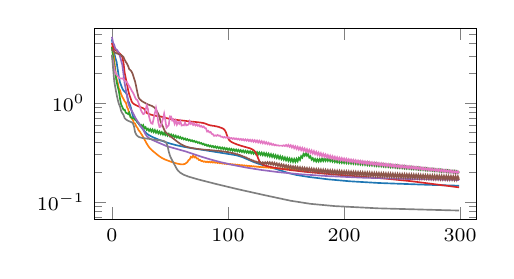
\begin{tikzpicture}

\definecolor{crimson2143940}{RGB}{214,39,40}
\definecolor{darkgray176}{RGB}{176,176,176}
\definecolor{darkorange25512714}{RGB}{255,127,14}
\definecolor{forestgreen4416044}{RGB}{44,160,44}
\definecolor{gray127}{RGB}{127,127,127}
\definecolor{mediumpurple148103189}{RGB}{148,103,189}
\definecolor{orchid227119194}{RGB}{227,119,194}
\definecolor{sienna1408675}{RGB}{140,86,75}
\definecolor{steelblue31119180}{RGB}{31,119,180}

\begin{axis}[compar,
	ymode=log]
\addplot [semithick, steelblue31119180]
table {%
0 4.40617990493774
1 3.69606566429138
2 3.2255163192749
3 2.84633851051331
4 2.62248873710632
5 2.18969368934631
6 1.84045720100403
7 1.61833596229553
8 1.50373470783234
9 1.40086615085602
10 1.33667957782745
11 1.30011606216431
12 1.26939678192139
13 1.21144664287567
14 1.05346322059631
15 0.994601011276245
16 0.930943489074707
17 0.838274955749512
18 0.737896680831909
19 0.707594513893127
20 0.683580040931702
22 0.64062762260437
26 0.557338953018188
28 0.520130634307861
29 0.504136919975281
30 0.491180896759033
31 0.481052398681641
33 0.465569615364075
36 0.447391867637634
40 0.427431344985962
45 0.406768202781677
50 0.389152765274048
55 0.375323534011841
61 0.362203121185303
69 0.348344445228577
81 0.331637144088745
107 0.296327710151672
112 0.284664392471313
117 0.268661975860596
122 0.253267884254456
127 0.241251468658447
134 0.228349685668945
145 0.208487987518311
152 0.195589780807495
159 0.187051057815552
169 0.178939342498779
186 0.169061064720154
205 0.161450624465942
230 0.155169367790222
271 0.148949861526489
299 0.145651340484619
};
\addplot [semithick, darkorange25512714]
table {%
0 3.73980402946472
1 3.27899599075317
2 2.78873038291931
3 2.1209659576416
4 1.75611484050751
5 1.61170637607574
6 1.39949643611908
7 1.34306573867798
8 1.22348916530609
9 1.15239131450653
10 1.09919130802155
11 1.03782510757446
12 1.01289129257202
13 0.913549900054932
14 0.862408518791199
15 0.775715112686157
17 0.696209669113159
18 0.676398992538452
19 0.62683629989624
20 0.618960380554199
21 0.578180313110352
22 0.561890244483948
23 0.530904054641724
24 0.51520037651062
25 0.492515325546265
26 0.473389029502869
29 0.408502221107483
30 0.388869047164917
31 0.371843576431274
32 0.357532978057861
33 0.346150517463684
35 0.328909754753113
39 0.300641179084778
41 0.288151860237122
43 0.278338313102722
46 0.267471432685852
51 0.254124760627747
56 0.244026899337769
59 0.239923715591431
61 0.239256143569946
63 0.242369890213013
65 0.252156257629395
66 0.264179229736328
67 0.268280625343323
68 0.285303711891174
69 0.281058669090271
70 0.294731020927429
71 0.281811475753784
72 0.28748083114624
73 0.274154663085938
74 0.275272607803345
75 0.265120506286621
76 0.265589952468872
77 0.258352041244507
78 0.259693503379822
79 0.254309177398682
80 0.256695508956909
81 0.252245664596558
82 0.255406618118286
83 0.251249432563782
84 0.254801511764526
85 0.250563621520996
86 0.254149675369263
87 0.249704599380493
88 0.253089547157288
89 0.248494267463684
90 0.251598119735718
91 0.246989965438843
92 0.24984872341156
93 0.245354533195496
94 0.248048782348633
95 0.243738532066345
96 0.246336460113525
97 0.242225050926208
98 0.244760751724243
99 0.240829110145569
100 0.243306398391724
101 0.239524722099304
102 0.241931080818176
103 0.238274216651917
104 0.240595102310181
105 0.237049102783203
106 0.239275932312012
107 0.235835790634155
108 0.23796808719635
109 0.234633803367615
110 0.236676931381226
111 0.233449578285217
112 0.235411524772644
113 0.232289791107178
114 0.234177827835083
115 0.231157898902893
116 0.232978224754333
117 0.230055093765259
118 0.231812000274658
119 0.228979587554932
120 0.230677008628845
121 0.227928996086121
122 0.229569554328918
123 0.226900458335876
124 0.228487968444824
125 0.225893259048462
126 0.227430582046509
127 0.224905133247375
128 0.226395964622498
129 0.223935723304749
130 0.225383281707764
131 0.222984075546265
132 0.224392056465149
133 0.222050070762634
134 0.223420977592468
135 0.221132397651672
136 0.222469687461853
137 0.220230460166931
138 0.22153639793396
139 0.219343066215515
140 0.220619916915894
141 0.218469023704529
142 0.219719529151917
143 0.217608332633972
144 0.218834519386292
145 0.21675968170166
146 0.217963695526123
147 0.215922117233276
148 0.217105746269226
149 0.215095281600952
150 0.216260552406311
151 0.214278340339661
152 0.215426921844482
153 0.213470697402954
154 0.214604377746582
155 0.212672114372253
156 0.213792324066162
157 0.211881875991821
158 0.212990164756775
159 0.2110995054245
160 0.212197184562683
161 0.21032440662384
162 0.211413145065308
163 0.209556698799133
164 0.210637450218201
165 0.20879602432251
166 0.209870457649231
167 0.20804226398468
168 0.209111571311951
169 0.207295536994934
170 0.208360910415649
171 0.206555366516113
172 0.207617998123169
173 0.205822467803955
174 0.206883907318115
175 0.205097079277039
176 0.206158399581909
177 0.204379558563232
178 0.205441832542419
179 0.203670144081116
180 0.204734802246094
181 0.202969312667847
182 0.204037547111511
183 0.202278017997742
184 0.20335066318512
185 0.201596260070801
186 0.202674746513367
187 0.200925350189209
188 0.202010750770569
189 0.200265526771545
190 0.201358795166016
191 0.199617505073547
192 0.200719714164734
193 0.198981881141663
194 0.200093388557434
195 0.198358058929443
196 0.199479579925537
197 0.197746753692627
198 0.198878407478333
199 0.197147488594055
200 0.19828999042511
201 0.196560740470886
202 0.19771420955658
203 0.195986270904541
204 0.197150707244873
205 0.195423364639282
206 0.196598410606384
207 0.194871187210083
208 0.196056604385376
209 0.194329500198364
210 0.195525169372559
211 0.193797826766968
212 0.195003032684326
213 0.193275332450867
214 0.194489598274231
215 0.192761182785034
216 0.193983912467957
217 0.192254781723022
218 0.193485379219055
219 0.191755771636963
220 0.192993402481079
221 0.191263198852539
222 0.19250750541687
223 0.190776824951172
224 0.192026972770691
225 0.190295934677124
226 0.191551446914673
227 0.189820647239685
228 0.191080927848816
229 0.189350008964539
230 0.190614223480225
231 0.188883662223816
232 0.190151214599609
233 0.188421368598938
234 0.18969190120697
235 0.187963008880615
236 0.189235925674438
237 0.187508463859558
238 0.188783407211304
239 0.187057495117188
240 0.188333749771118
241 0.186609625816345
242 0.187886714935303
243 0.186164617538452
244 0.187442302703857
245 0.185722827911377
246 0.187000751495361
247 0.185283899307251
248 0.186561584472656
249 0.184847831726074
250 0.186124801635742
251 0.184414744377136
252 0.185690879821777
253 0.183984398841858
254 0.185259342193604
255 0.183557033538818
256 0.1848304271698
257 0.183132290840149
258 0.184403896331787
259 0.182709932327271
260 0.183979392051697
261 0.182290315628052
262 0.183557629585266
263 0.181873798370361
264 0.183138489723206
265 0.18146014213562
266 0.182722449302673
267 0.181049585342407
268 0.182308912277222
269 0.180642247200012
270 0.181898713111877
271 0.180238246917725
272 0.181491255760193
273 0.179837226867676
274 0.181087017059326
275 0.179439783096313
276 0.180686235427856
277 0.179046273231506
278 0.180289030075073
279 0.178656458854675
280 0.179895520210266
281 0.178270936012268
282 0.179506182670593
283 0.177889585494995
284 0.179120779037476
285 0.177512526512146
286 0.178739786148071
287 0.1771399974823
288 0.178362607955933
289 0.176771998405457
290 0.177990198135376
291 0.176408648490906
292 0.177621841430664
293 0.176049470901489
294 0.177257537841797
295 0.175694823265076
296 0.176897883415222
297 0.175345420837402
298 0.176543235778809
299 0.175000905990601
};
\addplot [semithick, forestgreen4416044]
table {%
0 3.67940378189087
1 2.93019533157349
2 2.43471574783325
3 2.01281762123108
4 1.65761744976044
5 1.46219766139984
6 1.32063746452332
7 1.10604918003082
8 0.961245656013489
9 0.911208033561707
10 0.854409456253052
11 0.857123136520386
12 0.796026587486267
13 0.789343357086182
14 0.771284341812134
15 0.798981189727783
16 0.720513343811035
17 0.710151553153992
18 0.698009014129639
19 0.699390769004822
20 0.67522144317627
21 0.674743175506592
22 0.63738751411438
23 0.628534078598022
24 0.595621347427368
25 0.603557705879211
26 0.575085878372192
27 0.596360445022583
28 0.554007291793823
29 0.569077491760254
30 0.533450126647949
31 0.549681186676025
32 0.521344423294067
33 0.543054342269897
34 0.514695644378662
35 0.539749503135681
36 0.507904767990112
37 0.532358407974243
38 0.500342130661011
39 0.523404479026794
40 0.492777109146118
41 0.514869213104248
42 0.485900640487671
43 0.507613778114319
44 0.479504704475403
45 0.500825881958008
46 0.473396420478821
47 0.49415647983551
48 0.467438936233521
49 0.487385034561157
50 0.461739540100098
51 0.48060131072998
52 0.456370949745178
53 0.473809957504272
54 0.451216459274292
55 0.46695339679718
56 0.446010589599609
57 0.459914803504944
58 0.440494656562805
59 0.452619433403015
60 0.434565424919128
61 0.44519567489624
62 0.428452491760254
63 0.438084006309509
64 0.422637939453125
65 0.431661367416382
66 0.417298436164856
67 0.425767660140991
68 0.41215717792511
69 0.419995903968811
70 0.406880617141724
71 0.414074301719666
72 0.401265025138855
73 0.407877206802368
74 0.395194888114929
75 0.40132999420166
76 0.388608813285828
77 0.394424438476562
78 0.381601095199585
79 0.387405157089233
80 0.374626040458679
81 0.380896687507629
82 0.368383526802063
83 0.375481843948364
84 0.363188147544861
85 0.371125221252441
86 0.358786821365356
87 0.36739718914032
88 0.354832410812378
89 0.363967895507812
90 0.351144671440125
91 0.360710978507996
92 0.347663402557373
93 0.357593059539795
94 0.344362854957581
95 0.354593515396118
96 0.341216802597046
97 0.351688146591187
98 0.338198184967041
99 0.348856687545776
100 0.33528470993042
101 0.346090078353882
102 0.332459449768066
103 0.343386173248291
104 0.329710483551025
105 0.34074866771698
106 0.327028751373291
107 0.338183403015137
108 0.324407577514648
109 0.335696458816528
110 0.321841359138489
111 0.33329439163208
112 0.31932520866394
113 0.330983519554138
114 0.316855430603027
115 0.328768730163574
116 0.314427256584167
117 0.326651334762573
118 0.312034487724304
119 0.324625492095947
120 0.309666633605957
121 0.322674632072449
122 0.307306289672852
123 0.320764899253845
124 0.304927110671997
125 0.318843841552734
126 0.302493810653687
127 0.316841244697571
128 0.299965381622314
129 0.314680218696594
130 0.297302484512329
131 0.312294483184814
132 0.294477939605713
133 0.309645295143127
134 0.291482210159302
135 0.306729078292847
136 0.288322687149048
137 0.303571701049805
138 0.2850182056427
139 0.300215840339661
140 0.281589150428772
141 0.296704292297363
142 0.278052926063538
143 0.293073892593384
144 0.274423360824585
145 0.289357542991638
146 0.270718336105347
147 0.285593867301941
148 0.266972303390503
149 0.281844615936279
150 0.263256192207336
151 0.278220891952515
152 0.259711623191833
153 0.274926543235779
154 0.256603717803955
155 0.272324562072754
156 0.254412531852722
157 0.271059036254883
158 0.254010915756226
159 0.272284507751465
160 0.25695526599884
161 0.27791428565979
162 0.265474796295166
163 0.289864778518677
164 0.280057787895203
165 0.305453896522522
166 0.293200969696045
167 0.312587141990662
168 0.292814373970032
169 0.30359148979187
170 0.280547499656677
171 0.288453340530396
172 0.267788529396057
173 0.277171850204468
174 0.25978422164917
175 0.271487712860107
176 0.256303787231445
177 0.270045876502991
178 0.255953311920166
179 0.271146655082703
180 0.257334470748901
181 0.273201465606689
182 0.259106397628784
183 0.274811387062073
184 0.260095119476318
185 0.275022506713867
186 0.259649872779846
187 0.273645520210266
188 0.257884502410889
189 0.271212577819824
190 0.255439519882202
191 0.268505811691284
192 0.252985715866089
193 0.266096115112305
194 0.250914931297302
195 0.264199376106262
196 0.24931812286377
197 0.262762188911438
198 0.248097658157349
199 0.261608242988586
200 0.247086763381958
201 0.260550022125244
202 0.246127009391785
203 0.259450078010559
204 0.245111107826233
205 0.258241057395935
206 0.243993043899536
207 0.256916642189026
208 0.242778539657593
209 0.255511045455933
210 0.241503000259399
211 0.254071474075317
212 0.240208268165588
213 0.25263786315918
214 0.238928318023682
215 0.251236438751221
216 0.237681984901428
217 0.249874830245972
218 0.2364741563797
219 0.248550415039062
220 0.23530125617981
221 0.247255563735962
222 0.234154224395752
223 0.245979905128479
224 0.233024597167969
225 0.24471652507782
226 0.231904745101929
227 0.243459939956665
228 0.230790853500366
229 0.242208480834961
230 0.229681015014648
231 0.240962624549866
232 0.228575825691223
233 0.239723563194275
234 0.227476119995117
235 0.238492488861084
236 0.226383447647095
237 0.237271189689636
238 0.225299477577209
239 0.236060619354248
240 0.22422456741333
241 0.23486065864563
242 0.223159432411194
243 0.233672142028809
244 0.222103714942932
245 0.232494235038757
246 0.221056818962097
247 0.231325626373291
248 0.220017910003662
249 0.23016619682312
250 0.218986988067627
251 0.229015827178955
252 0.217963099479675
253 0.227873563766479
254 0.216946601867676
255 0.226739883422852
256 0.215936541557312
257 0.225613951683044
258 0.214933037757874
259 0.224496006965637
260 0.213936448097229
261 0.22338604927063
262 0.212945818901062
263 0.222282648086548
264 0.211960911750793
265 0.221186876296997
266 0.21098268032074
267 0.220098614692688
268 0.210010290145874
269 0.219017505645752
270 0.209043622016907
271 0.217943072319031
272 0.208082675933838
273 0.216875314712524
274 0.207127690315247
275 0.215814590454102
276 0.206178426742554
277 0.214760780334473
278 0.205234527587891
279 0.213712811470032
280 0.204295516014099
281 0.212671041488647
282 0.203361988067627
283 0.211635708808899
284 0.202433824539185
285 0.210606455802917
286 0.201510190963745
287 0.209582805633545
288 0.200591802597046
289 0.208565592765808
290 0.199678421020508
291 0.20755398273468
292 0.198769807815552
293 0.206547856330872
294 0.197865962982178
295 0.205548048019409
296 0.196967124938965
297 0.204553723335266
298 0.196073293685913
299 0.203565359115601
};
\addplot [semithick, crimson2143940]
table {%
0 4.03240489959717
1 3.66145968437195
2 3.50826072692871
3 3.43945097923279
4 3.40309906005859
5 3.29447650909424
6 3.23242688179016
7 3.15045285224915
8 3.06647610664368
9 2.90932965278625
10 2.54663157463074
11 2.02920961380005
12 1.76606631278992
13 1.5545746088028
14 1.34510231018066
15 1.21288168430328
16 1.12531435489655
17 1.03593420982361
18 0.998515844345093
19 0.976468920707703
21 0.946892976760864
23 0.922716379165649
27 0.885076999664307
28 0.867321729660034
30 0.794364929199219
31 0.781225919723511
33 0.76573657989502
36 0.748886823654175
38 0.740663290023804
39 0.736942887306213
40 0.73579216003418
41 0.731165885925293
42 0.73081111907959
43 0.723122477531433
44 0.72137713432312
45 0.712852239608765
46 0.709953904151917
47 0.702707290649414
48 0.699588298797607
49 0.693649888038635
50 0.69086766242981
51 0.685944795608521
52 0.683995485305786
53 0.679930448532104
54 0.679020643234253
55 0.675410509109497
56 0.675253748893738
57 0.671579360961914
58 0.67163610458374
59 0.667659759521484
60 0.667473316192627
61 0.663389682769775
62 0.662828207015991
63 0.65899658203125
64 0.658180952072144
65 0.654799342155457
66 0.65388035774231
67 0.650936365127563
70 0.646396160125732
73 0.640487194061279
75 0.636707663536072
77 0.632090330123901
78 0.629792928695679
80 0.621576428413391
83 0.602075576782227
85 0.593022704124451
86 0.591253280639648
87 0.587563276290894
88 0.586412191390991
89 0.582295060157776
90 0.580511331558228
91 0.575647592544556
92 0.572798848152161
95 0.555975675582886
96 0.548262357711792
97 0.534722566604614
98 0.512758255004883
100 0.441529989242554
101 0.421590447425842
102 0.411294341087341
103 0.403133153915405
106 0.388078808784485
108 0.380065679550171
111 0.369992971420288
119 0.3477783203125
121 0.339373111724854
122 0.333412289619446
123 0.325174927711487
124 0.313146591186523
125 0.29570484161377
126 0.274777770042419
127 0.258257389068604
128 0.248561859130859
129 0.24269437789917
131 0.235647439956665
134 0.229305744171143
140 0.221243858337402
150 0.212175130844116
166 0.201727867126465
190 0.189919352531433
232 0.173438787460327
258 0.161711931228638
299 0.140178918838501
};
\addplot [semithick, mediumpurple148103189]
table {%
0 4.66009426116943
1 4.09302425384521
2 3.8778133392334
3 3.52610301971436
4 3.47141408920288
5 3.36333274841309
6 3.20856022834778
7 2.94592428207397
8 2.67666721343994
9 2.41839456558228
10 1.95576667785645
11 1.58032274246216
12 1.36911773681641
13 1.18978691101074
14 1.0056711435318
15 0.931052088737488
16 0.876487016677856
18 0.799840211868286
20 0.718108415603638
21 0.684044122695923
23 0.628328561782837
24 0.603073358535767
27 0.536755919456482
29 0.482640266418457
30 0.464487671852112
31 0.451732635498047
32 0.441940784454346
34 0.427545189857483
37 0.412033319473267
47 0.366768598556519
51 0.355843067169189
64 0.322333216667175
77 0.286389470100403
85 0.268261909484863
94 0.251472353935242
104 0.236355066299438
116 0.22199285030365
129 0.20993709564209
144 0.19944441318512
162 0.190355777740479
185 0.182435870170593
215 0.175788044929504
259 0.169866561889648
299 0.166379451751709
};
\addplot [semithick, sienna1408675]
table {%
0 3.50270557403564
1 3.36141872406006
2 3.30206489562988
3 3.23297595977783
4 3.17998647689819
5 3.1468780040741
6 3.11884689331055
7 3.08162117004395
8 3.05721735954285
9 2.99129629135132
10 2.91612982749939
11 2.73877549171448
12 2.6012110710144
13 2.5010814666748
14 2.3608763217926
15 2.19062566757202
16 2.14710021018982
17 2.07490205764771
18 1.95372128486633
19 1.78838503360748
20 1.64641869068146
21 1.45485258102417
22 1.2709676027298
23 1.13231980800629
24 1.09220516681671
25 1.06450998783112
26 1.04094505310059
28 1.00996208190918
30 0.979291796684265
31 0.967232942581177
34 0.937765121459961
35 0.92590856552124
36 0.910855174064636
37 0.889240503311157
38 0.858229041099548
39 0.812992811203003
40 0.775282859802246
41 0.718624830245972
42 0.64487636089325
43 0.60725212097168
44 0.576647758483887
45 0.53918731212616
46 0.511808156967163
47 0.496371746063232
49 0.473034381866455
52 0.444973945617676
57 0.400668978691101
59 0.386002779006958
62 0.369724035263062
64 0.362025499343872
66 0.356427192687988
68 0.352195858955383
70 0.348816394805908
72 0.34598708152771
73 0.343830585479736
74 0.34353768825531
75 0.341451168060303
76 0.34136950969696
77 0.339308738708496
78 0.339421272277832
79 0.337348699569702
80 0.337650537490845
81 0.335530519485474
82 0.336022019386292
83 0.333818197250366
84 0.334500551223755
85 0.332175135612488
86 0.333045482635498
87 0.330559492111206
88 0.331608176231384
89 0.328922748565674
90 0.330130934715271
91 0.327210426330566
92 0.328548312187195
93 0.32536244392395
94 0.326790332794189
95 0.323316693305969
96 0.324785947799683
97 0.321011185646057
98 0.322466850280762
99 0.31838583946228
100 0.319769978523254
101 0.315382719039917
102 0.316637635231018
103 0.311946511268616
104 0.313019275665283
105 0.308025598526001
106 0.308873295783997
107 0.303575754165649
108 0.304173469543457
109 0.298569202423096
110 0.298922538757324
111 0.293010592460632
112 0.293167114257812
113 0.286948323249817
114 0.286999464035034
115 0.280468463897705
116 0.280538558959961
117 0.273686408996582
118 0.273932337760925
119 0.266793370246887
120 0.267447829246521
121 0.260168075561523
122 0.261555314064026
123 0.254336833953857
124 0.256779432296753
125 0.249709844589233
126 0.253453612327576
127 0.246416926383972
128 0.251643896102905
129 0.244331955909729
130 0.251141548156738
131 0.243105411529541
132 0.251431703567505
133 0.242207527160645
134 0.251762866973877
135 0.241079568862915
136 0.251419425010681
137 0.239363551139832
138 0.250062942504883
139 0.23702609539032
140 0.247823119163513
141 0.234275698661804
142 0.245086431503296
143 0.231382727622986
144 0.242231607437134
145 0.228553533554077
146 0.239500045776367
147 0.225895762443542
148 0.236991882324219
149 0.223439455032349
150 0.234713912010193
151 0.221169948577881
152 0.232630491256714
153 0.219056844711304
154 0.230696558952332
155 0.217069864273071
156 0.228874444961548
157 0.215186476707458
158 0.227141141891479
159 0.213393092155457
160 0.22548508644104
161 0.211682558059692
162 0.223901391029358
163 0.210050702095032
164 0.222388505935669
165 0.208494901657104
166 0.22094464302063
167 0.207012414932251
168 0.219568371772766
169 0.205599069595337
170 0.218255400657654
171 0.204251527786255
172 0.217002868652344
173 0.202965617179871
174 0.215806484222412
175 0.201737761497498
176 0.214663028717041
177 0.200564384460449
178 0.213569641113281
179 0.199442386627197
180 0.212522864341736
181 0.198368310928345
182 0.211519718170166
183 0.197339296340942
184 0.210557579994202
185 0.196353197097778
186 0.209634780883789
187 0.195407629013062
188 0.208748936653137
189 0.194499731063843
190 0.207897305488586
191 0.193627715110779
192 0.207078695297241
193 0.192789435386658
194 0.2062908411026
195 0.191982746124268
196 0.205531477928162
197 0.191205859184265
198 0.204799294471741
199 0.190456509590149
200 0.204092144966125
201 0.189733505249023
202 0.203408718109131
203 0.189034819602966
204 0.202747344970703
205 0.188359022140503
206 0.202106475830078
207 0.187704205513
208 0.201484322547913
209 0.187068939208984
210 0.200879216194153
211 0.186452031135559
212 0.20029079914093
213 0.18585216999054
214 0.199717044830322
215 0.185267210006714
216 0.199156165122986
217 0.184696674346924
218 0.198608160018921
219 0.184139728546143
220 0.198071956634521
221 0.183595299720764
222 0.197546243667603
223 0.183061599731445
224 0.197029590606689
225 0.182538270950317
226 0.196521759033203
227 0.182024478912354
228 0.196021795272827
229 0.181519865989685
230 0.195529460906982
231 0.181023001670837
232 0.195043325424194
233 0.180533647537231
234 0.194563150405884
235 0.18005108833313
236 0.194088578224182
237 0.179575204849243
238 0.193619728088379
239 0.179105877876282
240 0.193155646324158
241 0.17864191532135
242 0.19269597530365
243 0.178183436393738
244 0.192240476608276
245 0.177730202674866
246 0.191789031028748
247 0.177281379699707
248 0.191340804100037
249 0.17683732509613
250 0.190896272659302
251 0.176397800445557
252 0.190455436706543
253 0.175962328910828
254 0.190017223358154
255 0.175530791282654
256 0.189582228660583
257 0.175103187561035
258 0.189149618148804
259 0.174679160118103
260 0.188720107078552
261 0.174258947372437
262 0.188293695449829
263 0.173842787742615
264 0.187870144844055
265 0.1734299659729
266 0.187448859214783
267 0.173020362854004
268 0.187030553817749
269 0.172614693641663
270 0.186614990234375
271 0.172212362289429
272 0.186202049255371
273 0.171813011169434
274 0.185790777206421
275 0.171416521072388
276 0.185381889343262
277 0.171023368835449
278 0.184975624084473
279 0.17063319683075
280 0.184571385383606
281 0.170246124267578
282 0.184169769287109
283 0.169862031936646
284 0.183770537376404
285 0.169481158256531
286 0.1833735704422
287 0.169102907180786
288 0.182978630065918
289 0.168727517127991
290 0.182585954666138
291 0.168355107307434
292 0.182195663452148
293 0.167985439300537
294 0.181807637214661
295 0.167618751525879
296 0.181421637535095
297 0.167254328727722
298 0.181037306785583
299 0.166892647743225
};
\addplot [semithick, orchid227119194]
table {%
0 3.03507304191589
1 2.62677788734436
2 2.22404623031616
3 2.00302028656006
4 1.93074309825897
5 1.87389540672302
6 1.80747628211975
7 1.77715361118317
8 1.76992428302765
9 1.77597498893738
10 1.74454951286316
11 1.68282890319824
12 1.65570139884949
13 1.62520182132721
14 1.543288230896
15 1.47553563117981
16 1.41065907478333
17 1.3347202539444
18 1.28052401542664
19 1.21615839004517
20 1.13601493835449
21 1.08379185199738
22 1.06836462020874
24 0.928308963775635
25 0.84750509262085
26 0.803446292877197
27 0.772552013397217
28 0.780488610267639
29 0.852735757827759
30 0.943774461746216
31 0.873425006866455
32 0.731186389923096
33 0.657214283943176
34 0.621562004089355
35 0.616034984588623
36 0.697658061981201
38 0.891410946846008
39 0.776060461997986
40 0.634249567985535
41 0.572195053100586
42 0.57588255405426
43 0.631586670875549
44 0.693117141723633
45 0.779915809631348
46 0.674554228782654
47 0.56245231628418
49 0.598592042922974
50 0.732318043708801
51 0.729702234268188
52 0.664748072624207
53 0.681261539459229
54 0.616869926452637
55 0.665109992027283
56 0.604703903198242
57 0.641903519630432
58 0.618123531341553
59 0.655225038528442
60 0.591490745544434
61 0.596292018890381
62 0.593693733215332
63 0.632021546363831
64 0.59428858757019
66 0.605583906173706
67 0.652372717857361
68 0.613804340362549
69 0.631055116653442
70 0.599125742912292
71 0.618829250335693
72 0.593048930168152
73 0.610750913619995
74 0.587634205818176
75 0.598943710327148
76 0.577086925506592
77 0.586872935295105
78 0.569237470626831
79 0.579095840454102
80 0.559031248092651
81 0.555019855499268
82 0.514534711837769
83 0.522814512252808
84 0.504580974578857
85 0.509716749191284
86 0.487510442733765
87 0.483433365821838
88 0.465329051017761
89 0.470841288566589
90 0.46513032913208
91 0.475481271743774
92 0.465944886207581
93 0.46855354309082
94 0.45487916469574
95 0.456343412399292
96 0.446525573730469
97 0.453030943870544
98 0.445219993591309
99 0.452325344085693
100 0.442335367202759
101 0.447585582733154
102 0.436794757843018
103 0.442816615104675
104 0.432891488075256
105 0.4405357837677
106 0.43044650554657
107 0.438501238822937
108 0.427446365356445
109 0.435743570327759
110 0.424083352088928
111 0.43322229385376
112 0.421099424362183
113 0.431197166442871
114 0.4183030128479
115 0.42923104763031
116 0.415366888046265
117 0.427178502082825
118 0.41231381893158
119 0.425109267234802
120 0.409200310707092
121 0.422964930534363
122 0.405974149703979
123 0.420593738555908
124 0.402591228485107
125 0.417858719825745
126 0.399062275886536
127 0.414642095565796
128 0.395418643951416
129 0.410842895507812
130 0.391695499420166
131 0.406414031982422
132 0.38792896270752
133 0.401387453079224
134 0.384150743484497
135 0.395874261856079
136 0.380411148071289
137 0.390061616897583
138 0.376815915107727
139 0.384197950363159
140 0.373575806617737
141 0.378606081008911
142 0.371074557304382
143 0.373719334602356
144 0.369924306869507
146 0.370811820030212
147 0.368040919303894
148 0.373677611351013
149 0.366933822631836
150 0.376636505126953
151 0.364891171455383
152 0.376962900161743
153 0.360595941543579
154 0.37393581867218
155 0.354702711105347
156 0.369175434112549
157 0.348684906959534
158 0.36435079574585
159 0.343278169631958
160 0.35991644859314
161 0.338352680206299
162 0.355574131011963
163 0.333539485931396
164 0.351011157035828
165 0.328634858131409
166 0.346156597137451
167 0.323622584342957
168 0.341087937355042
169 0.318560004234314
170 0.33590304851532
171 0.313505172729492
172 0.330673933029175
173 0.308504819869995
174 0.325455188751221
175 0.30359947681427
176 0.320297360420227
177 0.298830032348633
178 0.315252780914307
179 0.294234752655029
180 0.310369729995728
181 0.289844989776611
182 0.305689454078674
183 0.285683512687683
184 0.301241159439087
185 0.281761765480042
186 0.297041416168213
187 0.278083086013794
188 0.293098092079163
189 0.274644255638123
190 0.289408206939697
191 0.27143406867981
192 0.285962581634521
193 0.268439292907715
194 0.282746911048889
195 0.26564347743988
196 0.279744863510132
197 0.263030052185059
198 0.276938438415527
199 0.260582447052002
200 0.274309039115906
201 0.258282542228699
202 0.271838068962097
203 0.256115078926086
204 0.269508361816406
205 0.254065275192261
206 0.267304182052612
207 0.252119541168213
208 0.26521098613739
209 0.250266194343567
210 0.26321542263031
211 0.248493432998657
212 0.261305212974548
213 0.246792197227478
214 0.25947105884552
215 0.245154619216919
216 0.25770378112793
217 0.24357283115387
218 0.255995035171509
219 0.242040038108826
220 0.254338145256042
221 0.240550398826599
222 0.252725839614868
223 0.23909866809845
224 0.251153469085693
225 0.237680792808533
226 0.249616742134094
227 0.236293435096741
228 0.248111486434937
229 0.234932541847229
230 0.246633887290955
231 0.233595609664917
232 0.245181560516357
233 0.232280492782593
234 0.243752241134644
235 0.230984926223755
236 0.242342829704285
237 0.229706764221191
238 0.240952253341675
239 0.228444814682007
240 0.239577889442444
241 0.227197051048279
242 0.238218784332275
243 0.225962519645691
244 0.236873269081116
245 0.224740266799927
246 0.235540628433228
247 0.223528861999512
248 0.234219551086426
249 0.222328186035156
250 0.232909679412842
251 0.221137285232544
252 0.231610298156738
253 0.219955682754517
254 0.230320453643799
255 0.218782544136047
256 0.229040145874023
257 0.217618346214294
258 0.227768898010254
259 0.216461896896362
260 0.226505756378174
261 0.215312838554382
262 0.225250363349915
263 0.214171171188354
264 0.224002838134766
265 0.213036060333252
266 0.222761988639832
267 0.211907505989075
268 0.221528649330139
269 0.210785388946533
270 0.220301866531372
271 0.209669947624207
272 0.219082355499268
273 0.208560824394226
274 0.217869520187378
275 0.207457661628723
276 0.216662406921387
277 0.20635998249054
278 0.215461730957031
279 0.205268621444702
280 0.214267492294312
281 0.204182624816895
282 0.213079214096069
283 0.203102707862854
284 0.211897611618042
285 0.202028870582581
286 0.210721969604492
287 0.200960397720337
288 0.209551930427551
289 0.199896931648254
290 0.20838737487793
291 0.198838710784912
292 0.207228422164917
293 0.197785615921021
294 0.206074953079224
295 0.196738004684448
296 0.204927802085876
297 0.195696115493774
298 0.203786373138428
299 0.194659352302551
};
\addplot [semithick, gray127]
table {%
0 3.07018613815308
1 2.26682066917419
2 1.66534912586212
3 1.42185187339783
4 1.22849655151367
5 1.08568918704987
6 0.979161262512207
7 0.920129299163818
8 0.82662034034729
9 0.787699699401855
10 0.757268786430359
11 0.703811645507812
12 0.683829307556152
13 0.670875430107117
14 0.660512685775757
17 0.638788104057312
18 0.624574661254883
19 0.583323955535889
20 0.506173968315125
21 0.478316783905029
22 0.464001893997192
23 0.454689860343933
24 0.449524879455566
26 0.443619251251221
30 0.436510682106018
44 0.415118813514709
45 0.411405444145203
46 0.405284881591797
47 0.393077611923218
48 0.365192174911499
49 0.321544408798218
50 0.294076204299927
51 0.275607228279114
54 0.237131357192993
55 0.224776268005371
56 0.214474439620972
57 0.206750154495239
59 0.196680426597595
62 0.187744379043579
66 0.180032253265381
74 0.169020652770996
90 0.151325583457947
108 0.134682416915894
131 0.117222309112549
154 0.102617263793945
171 0.0954985618591309
192 0.0906010866165161
229 0.0860358476638794
292 0.0820772647857666
299 0.0817854404449463
};
\end{axis}

\end{tikzpicture}
}
	&
	\multicolumn{5}{c}{% This file was created with tikzplotlib v0.10.1.
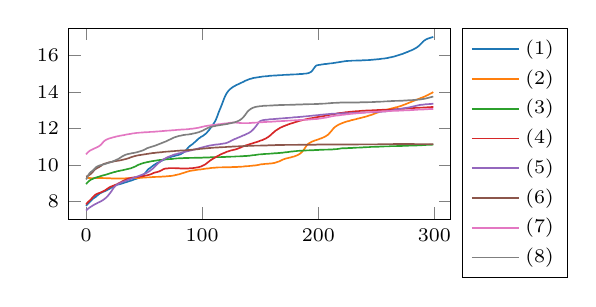
\begin{tikzpicture}

\definecolor{crimson2143940}{RGB}{214,39,40}
\definecolor{darkgray176}{RGB}{176,176,176}
\definecolor{darkorange25512714}{RGB}{255,127,14}
\definecolor{forestgreen4416044}{RGB}{44,160,44}
\definecolor{gray127}{RGB}{127,127,127}
\definecolor{mediumpurple148103189}{RGB}{148,103,189}
\definecolor{orchid227119194}{RGB}{227,119,194}
\definecolor{sienna1408675}{RGB}{140,86,75}
\definecolor{steelblue31119180}{RGB}{31,119,180}

\begin{axis}[compar, legend pos=outer north east]
\addplot [semithick, steelblue31119180]
table {%
0 7.76000022888184
1 7.84000015258789
2 7.90000009536743
3 7.96999979019165
4 8.02999973297119
5 8.10000038146973
6 8.15999984741211
8 8.23999977111816
9 8.28999996185303
10 8.35000038146973
12 8.44999980926514
15 8.53999996185303
16 8.5600004196167
18 8.61999988555908
19 8.65999984741211
20 8.6899995803833
24 8.85000038146973
25 8.88000011444092
28 8.9399995803833
29 8.94999980926514
40 9.17000007629395
41 9.19999980926514
45 9.27999973297119
46 9.3100004196167
47 9.35000038146973
48 9.39999961853027
49 9.4399995803833
50 9.5
51 9.56999969482422
53 9.72999954223633
54 9.78999996185303
55 9.82999992370605
58 9.97999954223633
61 10.1000003814697
63 10.1599998474121
64 10.1999998092651
68 10.3199996948242
69 10.3400001525879
71 10.3999996185303
75 10.4799995422363
76 10.4899997711182
78 10.5299997329712
79 10.539999961853
81 10.5799999237061
82 10.6099996566772
84 10.6899995803833
85 10.7399997711182
86 10.8000001907349
88 10.960000038147
89 11.0200004577637
90 11.0699996948242
91 11.1099996566772
92 11.1599998474121
93 11.2200002670288
94 11.2700004577637
97 11.4499998092651
98 11.4899997711182
99 11.539999961853
100 11.5699996948242
101 11.6099996566772
103 11.710000038147
104 11.7700004577637
105 11.8500003814697
106 11.9200000762939
107 12.0100002288818
108 12.0900001525879
109 12.1800003051758
111 12.3800001144409
112 12.5100002288818
113 12.6700000762939
114 12.8500003814697
115 13.0100002288818
116 13.1599998474121
117 13.3199996948242
119 13.6599998474121
120 13.8000001907349
121 13.9200000762939
122 14.0100002288818
123 14.0900001525879
124 14.1499996185303
126 14.25
127 14.289999961853
128 14.3199996948242
129 14.3599996566772
136 14.5699996948242
137 14.6099996566772
138 14.6300001144409
139 14.6599998474121
140 14.6800003051758
141 14.710000038147
142 14.7200002670288
144 14.7600002288818
153 14.8500003814697
154 14.8500003814697
155 14.8599996566772
156 14.8599996566772
158 14.8800001144409
159 14.8800001144409
160 14.8900003433228
161 14.8900003433228
162 14.8999996185303
164 14.8999996185303
165 14.9099998474121
166 14.9099998474121
167 14.9200000762939
169 14.9200000762939
170 14.9300003051758
172 14.9300003051758
173 14.9399995803833
175 14.9399995803833
176 14.9499998092651
178 14.9499998092651
179 14.960000038147
181 14.960000038147
182 14.9700002670288
183 14.9700002670288
184 14.9799995422363
186 14.9799995422363
188 15
189 15
191 15.0200004577637
192 15.039999961853
193 15.0699996948242
194 15.1099996566772
195 15.1800003051758
197 15.3599996566772
198 15.4300003051758
199 15.460000038147
206 15.5299997329712
207 15.5299997329712
210 15.5600004196167
211 15.5600004196167
224 15.6899995803833
225 15.6899995803833
226 15.6999998092651
228 15.6999998092651
229 15.710000038147
232 15.710000038147
233 15.7200002670288
237 15.7200002670288
238 15.7299995422363
240 15.7299995422363
241 15.7399997711182
243 15.7399997711182
244 15.75
245 15.75
246 15.7600002288818
247 15.7600002288818
248 15.7700004577637
249 15.7700004577637
251 15.789999961853
252 15.789999961853
255 15.8199996948242
256 15.8199996948242
260 15.8599996566772
261 15.8800001144409
263 15.8999996185303
264 15.9200000762939
265 15.9300003051758
273 16.0900001525879
274 16.1200008392334
275 16.1399993896484
276 16.1700000762939
277 16.1900005340576
279 16.25
280 16.2700004577637
282 16.3299999237061
283 16.3700008392334
284 16.3999996185303
285 16.4400005340576
287 16.5400009155273
288 16.6100006103516
289 16.6700000762939
290 16.7399997711182
291 16.7999992370605
293 16.8799991607666
294 16.9099998474121
299 17.0100002288818
};
\addlegendentry{\scriptsize{$(1)$}}
\addplot [semithick, darkorange25512714]
table {%
0 9.30000019073486
1 9.30000019073486
2 9.28999996185303
3 9.28999996185303
4 9.27999973297119
10 9.27999973297119
11 9.28999996185303
14 9.28999996185303
15 9.27999973297119
17 9.27999973297119
18 9.27000045776367
21 9.27000045776367
22 9.26000022888184
33 9.26000022888184
34 9.27000045776367
36 9.27000045776367
37 9.27999973297119
39 9.27999973297119
40 9.28999996185303
46 9.28999996185303
47 9.30000019073486
48 9.30000019073486
49 9.3100004196167
51 9.3100004196167
52 9.31999969482422
54 9.31999969482422
55 9.32999992370605
56 9.32999992370605
57 9.34000015258789
59 9.34000015258789
60 9.35000038146973
62 9.35000038146973
63 9.35999965667725
65 9.35999965667725
66 9.36999988555908
68 9.36999988555908
69 9.38000011444092
70 9.38000011444092
72 9.39999961853027
73 9.39999961853027
76 9.43000030517578
77 9.44999980926514
78 9.46000003814697
79 9.47999954223633
80 9.48999977111816
89 9.67000007629395
97 9.75
98 9.75
104 9.8100004196167
105 9.8100004196167
108 9.84000015258789
109 9.84000015258789
110 9.85000038146973
111 9.85000038146973
112 9.85999965667725
113 9.85999965667725
114 9.86999988555908
117 9.86999988555908
118 9.88000011444092
125 9.88000011444092
126 9.89000034332275
130 9.89000034332275
131 9.89999961853027
133 9.89999961853027
134 9.90999984741211
135 9.90999984741211
137 9.93000030517578
138 9.93000030517578
139 9.9399995803833
140 9.9399995803833
141 9.94999980926514
142 9.94999980926514
144 9.97000026702881
145 9.97000026702881
149 10.0100002288818
150 10.0299997329712
151 10.039999961853
152 10.039999961853
154 10.0600004196167
155 10.0600004196167
156 10.0699996948242
157 10.0699996948242
158 10.0799999237061
159 10.0799999237061
162 10.1099996566772
166 10.1899995803833
170 10.3100004196167
173 10.3699998855591
174 10.3800001144409
175 10.3999996185303
176 10.4099998474121
178 10.4499998092651
179 10.460000038147
180 10.4899997711182
181 10.5100002288818
183 10.5699996948242
184 10.6099996566772
185 10.6599998474121
186 10.7200002670288
187 10.789999961853
188 10.8800001144409
189 10.9799995422363
190 11.0699996948242
191 11.1400003433228
192 11.1899995803833
193 11.2200002670288
194 11.2600002288818
195 11.289999961853
196 11.3100004196167
197 11.3400001525879
200 11.3999996185303
201 11.4300003051758
203 11.4700002670288
206 11.5600004196167
208 11.6400003433228
209 11.6999998092651
211 11.8400001525879
213 12
214 12.0600004196167
215 12.1099996566772
217 12.1899995803833
220 12.2799997329712
221 12.3000001907349
222 12.3299999237061
225 12.3900003433228
226 12.3999996185303
229 12.460000038147
230 12.4700002670288
231 12.4899997711182
232 12.5
234 12.539999961853
235 12.5500001907349
236 12.5699996948242
237 12.5799999237061
239 12.6199998855591
240 12.6300001144409
247 12.7700004577637
248 12.8000001907349
249 12.8199996948242
250 12.8500003814697
252 12.8900003433228
253 12.9200000762939
257 13
258 13.0100002288818
259 13.0299997329712
260 13.039999961853
262 13.0799999237061
263 13.0900001525879
264 13.1099996566772
265 13.1199998855591
267 13.1599998474121
268 13.1700000762939
272 13.25
273 13.2799997329712
275 13.3199996948242
277 13.3800001144409
278 13.3999996185303
279 13.4300003051758
280 13.4499998092651
282 13.5100002288818
283 13.5299997329712
284 13.5600004196167
285 13.5799999237061
286 13.6099996566772
287 13.6300001144409
288 13.6599998474121
289 13.6800003051758
290 13.710000038147
291 13.7299995422363
295 13.8500003814697
296 13.8900003433228
298 13.9499998092651
299 13.9899997711182
};
\addlegendentry{\scriptsize{$(2)$}}
\addplot [semithick, forestgreen4416044]
table {%
0 8.94999980926514
1 9.02999973297119
3 9.14999961853027
4 9.1899995803833
7 9.27999973297119
15 9.4399995803833
16 9.44999980926514
24 9.60999965667725
25 9.61999988555908
27 9.65999984741211
29 9.68000030517578
30 9.69999980926514
32 9.72000026702881
33 9.73999977111816
34 9.75
35 9.77000045776367
36 9.77999973297119
37 9.80000019073486
38 9.8100004196167
39 9.82999992370605
40 9.85999965667725
41 9.88000011444092
43 9.9399995803833
44 9.97999954223633
45 10.0100002288818
46 10.0299997329712
47 10.0600004196167
50 10.1199998855591
51 10.1300001144409
52 10.1499996185303
54 10.1700000762939
55 10.1899995803833
64 10.2799997329712
65 10.2799997329712
67 10.3000001907349
68 10.3000001907349
69 10.3100004196167
70 10.3100004196167
71 10.3199996948242
72 10.3199996948242
73 10.3299999237061
74 10.3299999237061
76 10.3500003814697
77 10.3500003814697
78 10.3599996566772
79 10.3599996566772
80 10.3699998855591
83 10.3699998855591
84 10.3800001144409
88 10.3800001144409
89 10.3900003433228
93 10.3900003433228
94 10.3999996185303
100 10.3999996185303
101 10.4099998474121
106 10.4099998474121
107 10.4200000762939
111 10.4200000762939
112 10.4300003051758
116 10.4300003051758
117 10.4399995803833
120 10.4399995803833
121 10.4499998092651
124 10.4499998092651
125 10.460000038147
128 10.460000038147
129 10.4700002670288
132 10.4700002670288
133 10.4799995422363
135 10.4799995422363
136 10.4899997711182
138 10.4899997711182
140 10.5100002288818
141 10.5100002288818
144 10.539999961853
145 10.539999961853
149 10.5799999237061
150 10.5799999237061
151 10.5900001525879
152 10.5900001525879
153 10.6000003814697
154 10.6000003814697
155 10.6099996566772
157 10.6099996566772
158 10.6199998855591
159 10.6199998855591
160 10.6300001144409
161 10.6300001144409
162 10.6400003433228
164 10.6400003433228
166 10.6599998474121
167 10.6599998474121
168 10.6700000762939
169 10.6700000762939
172 10.6999998092651
173 10.6999998092651
177 10.7399997711182
178 10.7399997711182
180 10.7600002288818
181 10.7600002288818
182 10.7700004577637
183 10.7700004577637
184 10.7799997329712
186 10.7799997329712
187 10.789999961853
189 10.789999961853
190 10.8000001907349
192 10.8000001907349
193 10.8100004196167
196 10.8100004196167
197 10.8199996948242
200 10.8199996948242
201 10.8299999237061
204 10.8299999237061
205 10.8400001525879
208 10.8400001525879
209 10.8500003814697
212 10.8500003814697
213 10.8599996566772
214 10.8599996566772
215 10.8699998855591
216 10.8699998855591
221 10.9200000762939
225 10.9200000762939
226 10.9300003051758
229 10.9300003051758
230 10.9399995803833
232 10.9399995803833
233 10.9499998092651
235 10.9499998092651
236 10.960000038147
238 10.960000038147
239 10.9700002670288
241 10.9700002670288
242 10.9799995422363
244 10.9799995422363
245 10.9899997711182
248 10.9899997711182
249 11
252 11
253 11.0100002288818
256 11.0100002288818
257 11.0200004577637
261 11.0200004577637
262 11.0299997329712
267 11.0299997329712
268 11.039999961853
272 11.039999961853
273 11.0500001907349
277 11.0500001907349
278 11.0600004196167
281 11.0600004196167
282 11.0699996948242
285 11.0699996948242
286 11.0799999237061
289 11.0799999237061
290 11.0900001525879
292 11.0900001525879
293 11.1000003814697
295 11.1000003814697
296 11.1099996566772
298 11.1099996566772
299 11.1199998855591
};
\addlegendentry{\scriptsize{$(3)$}}
\addplot [semithick, crimson2143940]
table {%
0 7.84000015258789
1 7.92999982833862
4 8.10999965667725
6 8.25
8 8.36999988555908
9 8.40999984741211
10 8.4399995803833
12 8.47999954223633
16 8.60000038146973
17 8.64000034332275
18 8.6899995803833
21 8.8100004196167
22 8.82999992370605
23 8.85999965667725
24 8.88000011444092
25 8.90999984741211
26 8.93000030517578
27 8.96000003814697
28 9
30 9.0600004196167
31 9.10000038146973
36 9.25
37 9.27000045776367
38 9.27999973297119
39 9.30000019073486
42 9.32999992370605
43 9.32999992370605
50 9.39999961853027
51 9.42000007629395
53 9.4399995803833
56 9.5
58 9.5600004196167
60 9.60000038146973
61 9.60999965667725
63 9.64999961853027
65 9.71000003814697
66 9.75
67 9.77999973297119
68 9.80000019073486
69 9.8100004196167
70 9.8100004196167
72 9.82999992370605
76 9.82999992370605
77 9.81999969482422
80 9.81999969482422
81 9.8100004196167
88 9.8100004196167
89 9.81999969482422
91 9.81999969482422
97 9.88000011444092
99 9.92000007629395
102 10.0100002288818
103 10.0500001907349
107 10.25
111 10.4099998474121
112 10.4399995803833
113 10.4799995422363
114 10.5100002288818
115 10.5500001907349
118 10.6400003433228
119 10.6599998474121
121 10.7200002670288
125 10.8000001907349
126 10.8100004196167
127 10.8299999237061
128 10.8400001525879
131 10.8999996185303
132 10.9300003051758
133 10.9499998092651
135 11.0100002288818
136 11.0299997329712
137 11.0600004196167
149 11.3000001907349
150 11.3299999237061
152 11.3699998855591
155 11.460000038147
157 11.539999961853
159 11.6400003433228
161 11.7600002288818
162 11.8100004196167
163 11.8699998855591
167 12.0299997329712
170 12.1199998855591
171 12.1400003433228
172 12.1700000762939
173 12.1899995803833
174 12.2200002670288
184 12.4200000762939
185 12.4300003051758
187 12.4700002670288
188 12.4799995422363
189 12.5
191 12.5200004577637
192 12.539999961853
196 12.5799999237061
197 12.6000003814697
205 12.6800003051758
206 12.6999998092651
209 12.7299995422363
210 12.75
215 12.8000001907349
216 12.8199996948242
219 12.8500003814697
220 12.8500003814697
224 12.8900003433228
225 12.8900003433228
227 12.9099998474121
228 12.9099998474121
230 12.9300003051758
231 12.9300003051758
232 12.9399995803833
233 12.9399995803833
234 12.9499998092651
235 12.9499998092651
236 12.960000038147
237 12.960000038147
238 12.9700002670288
240 12.9700002670288
241 12.9799995422363
242 12.9799995422363
243 12.9899997711182
246 12.9899997711182
247 13
250 13
251 13.0100002288818
254 13.0100002288818
255 13.0200004577637
258 13.0200004577637
259 13.0299997329712
262 13.0299997329712
263 13.039999961853
265 13.039999961853
266 13.0500001907349
267 13.0500001907349
268 13.0600004196167
270 13.0600004196167
271 13.0699996948242
272 13.0699996948242
273 13.0799999237061
274 13.0799999237061
275 13.0900001525879
276 13.0900001525879
277 13.1000003814697
278 13.1000003814697
279 13.1099996566772
281 13.1099996566772
282 13.1199998855591
283 13.1199998855591
284 13.1300001144409
287 13.1300001144409
288 13.1400003433228
290 13.1400003433228
291 13.1499996185303
293 13.1499996185303
294 13.1599998474121
296 13.1599998474121
297 13.1700000762939
299 13.1700000762939
};
\addlegendentry{\scriptsize{$(4)$}}
\addplot [semithick, mediumpurple148103189]
table {%
0 7.51000022888184
1 7.57000017166138
3 7.67000007629395
7 7.82999992370605
9 7.8899998664856
10 7.92999982833862
13 8.02000045776367
15 8.10000038146973
17 8.19999980926514
18 8.26000022888184
19 8.32999992370605
21 8.48999977111816
22 8.57999992370605
23 8.68000030517578
24 8.77000045776367
25 8.84000015258789
26 8.89999961853027
27 8.9399995803833
31 9.0600004196167
32 9.07999992370605
33 9.10999965667725
35 9.14999961853027
36 9.18000030517578
38 9.22000026702881
39 9.25
40 9.27000045776367
41 9.30000019073486
43 9.34000015258789
44 9.36999988555908
46 9.40999984741211
47 9.4399995803833
48 9.46000003814697
49 9.48999977111816
50 9.51000022888184
53 9.60000038146973
55 9.68000030517578
58 9.82999992370605
59 9.89999961853027
60 9.96000003814697
61 10.0299997329712
62 10.0900001525879
65 10.2399997711182
67 10.3199996948242
68 10.3500003814697
69 10.3900003433228
71 10.4499998092651
72 10.4700002670288
73 10.5
74 10.5200004577637
75 10.5500001907349
77 10.5900001525879
78 10.6000003814697
80 10.6400003433228
81 10.6499996185303
83 10.6899995803833
84 10.6999998092651
85 10.7200002670288
86 10.7299995422363
87 10.75
88 10.7600002288818
89 10.7799997329712
90 10.789999961853
92 10.8299999237061
93 10.8400001525879
95 10.8800001144409
96 10.8900003433228
99 10.9499998092651
100 10.960000038147
102 11
103 11.0100002288818
104 11.0299997329712
105 11.039999961853
106 11.0600004196167
112 11.1199998855591
113 11.1199998855591
120 11.1899995803833
122 11.2299995422363
124 11.289999961853
125 11.3299999237061
128 11.4200000762939
129 11.4399995803833
131 11.5
132 11.5200004577637
135 11.6099996566772
136 11.6300001144409
140 11.75
142 11.8299999237061
144 11.9499998092651
145 12.0200004577637
147 12.1800003051758
148 12.2700004577637
149 12.3500003814697
150 12.4099998474121
152 12.4499998092651
155 12.4799995422363
156 12.4799995422363
158 12.5
159 12.5
160 12.5100002288818
161 12.5100002288818
162 12.5200004577637
163 12.5200004577637
164 12.5299997329712
165 12.5299997329712
166 12.539999961853
167 12.539999961853
168 12.5500001907349
169 12.5500001907349
170 12.5600004196167
171 12.5600004196167
172 12.5699996948242
173 12.5699996948242
174 12.5799999237061
175 12.5799999237061
176 12.5900001525879
177 12.5900001525879
179 12.6099996566772
180 12.6099996566772
181 12.6199998855591
182 12.6199998855591
183 12.6300001144409
184 12.6300001144409
185 12.6400003433228
186 12.6400003433228
188 12.6599998474121
189 12.6599998474121
190 12.6700000762939
191 12.6700000762939
193 12.6899995803833
194 12.6899995803833
196 12.710000038147
197 12.710000038147
199 12.7299995422363
200 12.7299995422363
202 12.75
203 12.75
205 12.7700004577637
206 12.7700004577637
207 12.7799997329712
208 12.7799997329712
209 12.789999961853
210 12.789999961853
211 12.8000001907349
213 12.8000001907349
214 12.8100004196167
216 12.8100004196167
217 12.8199996948242
220 12.8199996948242
221 12.8299999237061
224 12.8299999237061
225 12.8400001525879
229 12.8400001525879
230 12.8500003814697
233 12.8500003814697
234 12.8599996566772
237 12.8599996566772
238 12.8699998855591
240 12.8699998855591
241 12.8800001144409
244 12.8800001144409
245 12.8900003433228
248 12.8900003433228
249 12.8999996185303
251 12.8999996185303
252 12.9099998474121
254 12.9099998474121
255 12.9200000762939
256 12.9200000762939
257 12.9300003051758
258 12.9300003051758
265 13
266 13.0200004577637
267 13.0299997329712
268 13.0500001907349
279 13.1599998474121
280 13.1800003051758
281 13.1899995803833
282 13.210000038147
283 13.2200002670288
284 13.2399997711182
285 13.25
286 13.2700004577637
289 13.3000001907349
290 13.3000001907349
292 13.3199996948242
293 13.3199996948242
294 13.3299999237061
295 13.3299999237061
296 13.3400001525879
297 13.3400001525879
298 13.3500003814697
299 13.3500003814697
};
\addlegendentry{\scriptsize{$(5)$}}
\addplot [semithick, sienna1408675]
table {%
0 9.35999965667725
2 9.42000007629395
3 9.46000003814697
4 9.51000022888184
5 9.56999969482422
7 9.71000003814697
8 9.77000045776367
10 9.85000038146973
11 9.88000011444092
13 9.96000003814697
14 10.0200004577637
15 10.0500001907349
20 10.1499996185303
23 10.1800003051758
24 10.1999998092651
30 10.2600002288818
31 10.2799997329712
32 10.289999961853
33 10.3100004196167
34 10.3199996948242
37 10.3800001144409
38 10.4099998474121
42 10.4899997711182
43 10.5
44 10.5200004577637
58 10.6599998474121
59 10.6599998474121
61 10.6800003051758
62 10.6800003051758
64 10.6999998092651
65 10.6999998092651
67 10.7200002670288
68 10.7200002670288
69 10.7299995422363
70 10.7299995422363
71 10.7399997711182
72 10.7399997711182
73 10.75
74 10.75
75 10.7600002288818
76 10.7600002288818
77 10.7700004577637
78 10.7700004577637
79 10.7799997329712
80 10.7799997329712
81 10.789999961853
83 10.789999961853
84 10.8000001907349
85 10.8000001907349
86 10.8100004196167
87 10.8100004196167
88 10.8199996948242
89 10.8199996948242
90 10.8299999237061
91 10.8299999237061
93 10.8500003814697
94 10.8500003814697
95 10.8599996566772
96 10.8599996566772
98 10.8800001144409
99 10.8800001144409
101 10.8999996185303
102 10.8999996185303
104 10.9200000762939
105 10.9200000762939
106 10.9300003051758
107 10.9300003051758
108 10.9399995803833
109 10.9399995803833
110 10.9499998092651
111 10.9499998092651
112 10.960000038147
114 10.960000038147
115 10.9700002670288
117 10.9700002670288
118 10.9799995422363
120 10.9799995422363
121 10.9899997711182
122 10.9899997711182
123 11
125 11
126 11.0100002288818
128 11.0100002288818
129 11.0200004577637
131 11.0200004577637
132 11.0299997329712
135 11.0299997329712
136 11.039999961853
139 11.039999961853
140 11.0500001907349
144 11.0500001907349
145 11.0600004196167
150 11.0600004196167
151 11.0699996948242
156 11.0699996948242
157 11.0799999237061
162 11.0799999237061
163 11.0900001525879
170 11.0900001525879
171 11.1000003814697
182 11.1000003814697
183 11.1099996566772
198 11.1099996566772
199 11.1199998855591
234 11.1199998855591
235 11.1300001144409
251 11.1300001144409
252 11.1400003433228
264 11.1400003433228
265 11.1499996185303
282 11.1499996185303
283 11.1400003433228
299 11.1400003433228
};
\addlegendentry{\scriptsize{$(6)$}}
\addplot [semithick, orchid227119194]
table {%
0 10.5799999237061
1 10.6599998474121
2 10.7200002670288
3 10.7700004577637
4 10.8100004196167
11 11.0200004577637
13 11.1199998855591
14 11.1999998092651
15 11.2700004577637
16 11.3299999237061
17 11.3699998855591
19 11.4300003051758
23 11.5100002288818
24 11.5200004577637
26 11.5600004196167
28 11.5799999237061
29 11.6000003814697
33 11.6400003433228
34 11.6599998474121
39 11.710000038147
40 11.7299995422363
41 11.7299995422363
44 11.7600002288818
45 11.7600002288818
46 11.7700004577637
47 11.7700004577637
48 11.7799997329712
49 11.7799997329712
50 11.789999961853
52 11.789999961853
53 11.8000001907349
54 11.8000001907349
55 11.8100004196167
57 11.8100004196167
58 11.8199996948242
59 11.8199996948242
60 11.8299999237061
61 11.8299999237061
62 11.8400001525879
63 11.8400001525879
64 11.8500003814697
65 11.8500003814697
66 11.8599996566772
67 11.8599996566772
68 11.8699998855591
69 11.8699998855591
70 11.8800001144409
71 11.8800001144409
72 11.8900003433228
73 11.8900003433228
74 11.8999996185303
75 11.8999996185303
76 11.9099998474121
77 11.9099998474121
78 11.9200000762939
79 11.9200000762939
80 11.9300003051758
81 11.9300003051758
82 11.9399995803833
84 11.9399995803833
85 11.9499998092651
86 11.9499998092651
87 11.960000038147
88 11.960000038147
90 11.9799995422363
91 11.9799995422363
97 12.039999961853
98 12.0600004196167
99 12.0699996948242
100 12.0900001525879
101 12.1000003814697
102 12.1199998855591
109 12.1899995803833
110 12.1899995803833
114 12.2299995422363
115 12.2299995422363
119 12.2700004577637
120 12.2700004577637
125 12.3199996948242
126 12.3199996948242
127 12.3299999237061
128 12.3199996948242
129 12.3199996948242
130 12.3100004196167
131 12.3100004196167
132 12.3000001907349
133 12.3000001907349
134 12.289999961853
140 12.289999961853
141 12.3000001907349
142 12.3000001907349
143 12.3100004196167
145 12.3100004196167
146 12.3199996948242
147 12.3199996948242
148 12.3299999237061
150 12.3299999237061
151 12.3400001525879
152 12.3400001525879
153 12.3500003814697
155 12.3500003814697
156 12.3599996566772
158 12.3599996566772
159 12.3699998855591
160 12.3699998855591
161 12.3800001144409
163 12.3800001144409
164 12.3900003433228
166 12.3900003433228
167 12.3999996185303
168 12.3999996185303
169 12.4099998474121
171 12.4099998474121
172 12.4200000762939
173 12.4200000762939
174 12.4300003051758
176 12.4300003051758
177 12.4399995803833
179 12.4399995803833
180 12.4499998092651
182 12.4499998092651
183 12.460000038147
185 12.460000038147
186 12.4700002670288
188 12.4700002670288
189 12.4799995422363
191 12.4799995422363
192 12.4899997711182
193 12.4899997711182
194 12.5
195 12.5
196 12.5100002288818
197 12.5100002288818
198 12.5200004577637
199 12.5200004577637
207 12.6000003814697
208 12.6199998855591
210 12.6400003433228
211 12.6599998474121
216 12.710000038147
217 12.710000038147
221 12.75
222 12.75
225 12.7799997329712
226 12.7799997329712
228 12.8000001907349
229 12.8000001907349
231 12.8199996948242
232 12.8199996948242
233 12.8299999237061
234 12.8299999237061
236 12.8500003814697
237 12.8500003814697
238 12.8599996566772
239 12.8599996566772
241 12.8800001144409
242 12.8800001144409
243 12.8900003433228
244 12.8900003433228
245 12.8999996185303
246 12.8999996185303
247 12.9099998474121
248 12.9099998474121
249 12.9200000762939
251 12.9200000762939
252 12.9300003051758
254 12.9300003051758
255 12.9399995803833
258 12.9399995803833
259 12.9499998092651
262 12.9499998092651
263 12.960000038147
266 12.960000038147
267 12.9700002670288
269 12.9700002670288
270 12.9799995422363
273 12.9799995422363
274 12.9899997711182
276 12.9899997711182
277 13
279 13
280 13.0100002288818
282 13.0100002288818
283 13.0200004577637
285 13.0200004577637
286 13.0299997329712
288 13.0299997329712
289 13.039999961853
291 13.039999961853
292 13.0500001907349
294 13.0500001907349
295 13.0600004196167
298 13.0600004196167
299 13.0699996948242
};
\addlegendentry{\scriptsize{$(7)$}}
\addplot [semithick, gray127]
table {%
0 9.21000003814697
1 9.32999992370605
2 9.46000003814697
3 9.55000019073486
4 9.60999965667725
6 9.71000003814697
7 9.77000045776367
8 9.84000015258789
9 9.89999961853027
11 9.96000003814697
13 10
14 10.0100002288818
22 10.1700000762939
23 10.1999998092651
24 10.2200002670288
28 10.3400001525879
30 10.4200000762939
31 10.4700002670288
34 10.5600004196167
36 10.6000003814697
38 10.6199998855591
39 10.6400003433228
42 10.6700000762939
43 10.6899995803833
44 10.6999998092651
49 10.8000001907349
51 10.8599996566772
52 10.8999996185303
53 10.9300003051758
60 11.0699996948242
61 11.1000003814697
62 11.1199998855591
63 11.1499996185303
64 11.1700000762939
65 11.1999998092651
66 11.2200002670288
67 11.25
68 11.2700004577637
76 11.5100002288818
80 11.5900001525879
82 11.6099996566772
83 11.6300001144409
86 11.6599998474121
87 11.6599998474121
91 11.6999998092651
92 11.7200002670288
94 11.7399997711182
96 11.7799997329712
97 11.789999961853
98 11.8199996948242
99 11.8400001525879
101 11.8999996185303
102 11.9399995803833
106 12.0600004196167
107 12.0799999237061
108 12.0900001525879
109 12.1099996566772
111 12.1300001144409
112 12.1499996185303
122 12.25
123 12.2700004577637
125 12.289999961853
126 12.3100004196167
127 12.3199996948242
130 12.3800001144409
132 12.4399995803833
133 12.4799995422363
134 12.5299997329712
135 12.5900001525879
136 12.6599998474121
137 12.7399997711182
139 12.9200000762939
140 12.9799995422363
142 13.0799999237061
144 13.1400003433228
146 13.1800003051758
150 13.2200002670288
151 13.2200002670288
153 13.2399997711182
155 13.2399997711182
156 13.25
158 13.25
159 13.2600002288818
161 13.2600002288818
162 13.2700004577637
165 13.2700004577637
166 13.2799997329712
170 13.2799997329712
171 13.289999961853
175 13.289999961853
176 13.3000001907349
180 13.3000001907349
181 13.3100004196167
186 13.3100004196167
187 13.3199996948242
191 13.3199996948242
192 13.3299999237061
196 13.3299999237061
197 13.3400001525879
200 13.3400001525879
201 13.3500003814697
203 13.3500003814697
204 13.3599996566772
206 13.3599996566772
207 13.3699998855591
208 13.3699998855591
209 13.3800001144409
210 13.3800001144409
211 13.3900003433228
212 13.3900003433228
213 13.3999996185303
215 13.3999996185303
216 13.4099998474121
218 13.4099998474121
219 13.4200000762939
235 13.4200000762939
236 13.4300003051758
242 13.4300003051758
243 13.4399995803833
246 13.4399995803833
247 13.4499998092651
249 13.4499998092651
250 13.460000038147
253 13.460000038147
254 13.4700002670288
256 13.4700002670288
257 13.4799995422363
259 13.4799995422363
260 13.4899997711182
262 13.4899997711182
263 13.5
265 13.5
266 13.5100002288818
269 13.5100002288818
270 13.5200004577637
273 13.5200004577637
274 13.5299997329712
276 13.5299997329712
277 13.539999961853
279 13.539999961853
280 13.5500001907349
281 13.5500001907349
282 13.5600004196167
283 13.5600004196167
284 13.5699996948242
285 13.5699996948242
286 13.5799999237061
287 13.5799999237061
292 13.6300001144409
293 13.6499996185303
294 13.6599998474121
296 13.6999998092651
297 13.710000038147
298 13.7299995422363
299 13.7399997711182
};
\addlegendentry{\scriptsize{$(8)$}}
\end{axis}

\end{tikzpicture}
}
\end{tabular}
    \caption{Plein de descentes ---  avec passe-bas gaussien ($\sigma=0.6$)}
    \label{fig:LGDgauss-g}
\end{figure}

%\begin{figure}[H]\centering
	%\begin{tabular}{c c c c c c c c}
	$(1)$  &  $(2)$  &  $(3)$  &  $(4)$  &  $(5)$  &  $(6)$  &  $(7)$  &  $(8)$
	
	\\
	
	\includegraphics[width=0.1\textwidth]{resultats/LGD/multitarget/unif_1-init-pas=0.05_filtre=s-None}
	&
	\includegraphics[width=0.1\textwidth]{resultats/LGD/multitarget/unif_2-init-pas=0.05_filtre=s-None}
	&
	\includegraphics[width=0.1\textwidth]{resultats/LGD/multitarget/unif_3-init-pas=0.05_filtre=s-None}
	&
	\includegraphics[width=0.1\textwidth]{resultats/LGD/multitarget/unif_4-init-pas=0.05_filtre=s-None}
	&
	\includegraphics[width=0.1\textwidth]{resultats/LGD/multitarget/unif_5-init-pas=0.05_filtre=s-None}
	&
	\includegraphics[width=0.1\textwidth]{resultats/LGD/multitarget/unif_6-init-pas=0.05_filtre=s-None}
	&
	\includegraphics[width=0.1\textwidth]{resultats/LGD/multitarget/unif_7-init-pas=0.05_filtre=s-None}
	&
	\includegraphics[width=0.1\textwidth]{resultats/LGD/multitarget/unif_8-init-pas=0.05_filtre=s-None}
	
	\\
	
	\includegraphics[width=0.1\textwidth]{resultats/LGD/multitarget/unif_1-guess-pas=0.05_filtre=s-None}
	&
	\includegraphics[width=0.1\textwidth]{resultats/LGD/multitarget/unif_2-guess-pas=0.05_filtre=s-None}
	&
	\includegraphics[width=0.1\textwidth]{resultats/LGD/multitarget/unif_3-guess-pas=0.05_filtre=s-None}
	&
	\includegraphics[width=0.1\textwidth]{resultats/LGD/multitarget/unif_4-guess-pas=0.05_filtre=s-None}
	&
	\includegraphics[width=0.1\textwidth]{resultats/LGD/multitarget/unif_5-guess-pas=0.05_filtre=s-None}
	&
	\includegraphics[width=0.1\textwidth]{resultats/LGD/multitarget/unif_6-guess-pas=0.05_filtre=s-None}
	&
	\includegraphics[width=0.1\textwidth]{resultats/LGD/multitarget/unif_7-guess-pas=0.05_filtre=s-None}
	&
	\includegraphics[width=0.1\textwidth]{resultats/LGD/multitarget/unif_8-guess-pas=0.05_filtre=s-None}
	
	\\
	
	\includegraphics[width=0.1\textwidth]{resultats/LGD/multitarget/unif_1-target-pas=0.05_filtre=s-None}
	&
	\includegraphics[width=0.1\textwidth]{resultats/LGD/multitarget/unif_2-target-pas=0.05_filtre=s-None}
	&
	\includegraphics[width=0.1\textwidth]{resultats/LGD/multitarget/unif_3-target-pas=0.05_filtre=s-None}
	&
	\includegraphics[width=0.1\textwidth]{resultats/LGD/multitarget/unif_4-target-pas=0.05_filtre=s-None}
	&
	\includegraphics[width=0.1\textwidth]{resultats/LGD/multitarget/unif_5-target-pas=0.05_filtre=s-None}
	&
	\includegraphics[width=0.1\textwidth]{resultats/LGD/multitarget/unif_6-target-pas=0.05_filtre=s-None}
	&
	\includegraphics[width=0.1\textwidth]{resultats/LGD/multitarget/unif_7-target-pas=0.05_filtre=s-None}
	&
	\includegraphics[width=0.1\textwidth]{resultats/LGD/multitarget/unif_8-target-pas=0.05_filtre=s-None}
	
	\\ \\
	
	
	
	\multicolumn{2}{c}{Loss}  &  \multicolumn{4}{c}{PSNR{\color{white}bbbb}}
	
	\\
	
	\multicolumn{2}{c}{% This file was created with tikzplotlib v0.10.1.
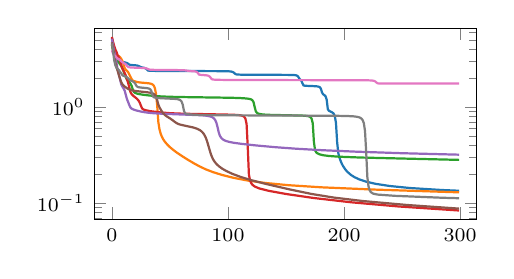
\begin{tikzpicture}

\definecolor{crimson2143940}{RGB}{214,39,40}
\definecolor{darkgray176}{RGB}{176,176,176}
\definecolor{darkorange25512714}{RGB}{255,127,14}
\definecolor{forestgreen4416044}{RGB}{44,160,44}
\definecolor{gray127}{RGB}{127,127,127}
\definecolor{mediumpurple148103189}{RGB}{148,103,189}
\definecolor{orchid227119194}{RGB}{227,119,194}
\definecolor{sienna1408675}{RGB}{140,86,75}
\definecolor{steelblue31119180}{RGB}{31,119,180}

\begin{axis}[compar,
	ymode=log]
\addplot [thick, steelblue31119180]
table {%
0 5.28534698486328
1 4.56153583526611
2 4.15292692184448
3 3.77370262145996
4 3.47898125648499
5 3.31976199150085
6 3.19493985176086
7 3.10722255706787
8 3.03175711631775
9 2.97216963768005
10 2.94989323616028
12 2.91763210296631
13 2.89196872711182
14 2.84459686279297
15 2.78304696083069
16 2.76125717163086
17 2.75360822677612
20 2.73654866218567
21 2.72841548919678
22 2.7157461643219
23 2.69315505027771
25 2.61465978622437
26 2.59747767448425
27 2.58550000190735
28 2.57104706764221
29 2.54467082023621
30 2.48471784591675
31 2.41675543785095
32 2.40443253517151
34 2.39707183837891
37 2.39240050315857
43 2.38842940330505
56 2.38508582115173
95 2.37702870368958
99 2.37219524383545
101 2.3663010597229
102 2.36077666282654
103 2.35122561454773
104 2.33280158042908
105 2.29480004310608
106 2.23531317710876
107 2.20305252075195
108 2.19411134719849
110 2.18735361099243
113 2.18347454071045
120 2.18023037910461
142 2.17671942710876
152 2.17329335212708
155 2.16992664337158
157 2.16440415382385
158 2.15848612785339
159 2.1463565826416
160 2.11564350128174
161 2.03211307525635
162 1.95217657089233
163 1.90615499019623
164 1.79179537296295
165 1.68968415260315
166 1.67894756793976
168 1.67080318927765
172 1.66327273845673
175 1.65709567070007
177 1.64831936359406
178 1.63878691196442
179 1.61808812618256
180 1.56098234653473
181 1.42287838459015
182 1.36243319511414
183 1.33858788013458
184 1.30298972129822
185 1.19579434394836
186 0.949332118034363
187 0.917175769805908
190 0.879632592201233
191 0.857038736343384
192 0.809222936630249
193 0.683176517486572
194 0.432179570198059
195 0.332457780838013
196 0.298513174057007
197 0.275679111480713
198 0.258496284484863
199 0.244974851608276
201 0.225065946578979
203 0.211152195930481
206 0.196685552597046
209 0.186670541763306
213 0.177221775054932
219 0.167648196220398
227 0.159289002418518
239 0.151263952255249
257 0.143872141838074
284 0.137304782867432
299 0.13481867313385
};
\addplot [thick, darkorange25512714]
table {%
0 4.50131416320801
1 3.95711445808411
2 3.67994379997253
3 3.55212593078613
4 3.48827695846558
5 3.45385670661926
6 3.41005182266235
7 3.32293748855591
8 3.20924520492554
9 3.04128003120422
10 2.79263401031494
11 2.56510400772095
12 2.45271468162537
13 2.39788055419922
14 2.31529831886292
15 2.19441223144531
16 2.07752537727356
17 1.9688333272934
18 1.89682364463806
19 1.87376499176025
20 1.85760772228241
22 1.83091926574707
23 1.82071053981781
25 1.80813956260681
31 1.78046262264252
32 1.7734591960907
33 1.76414728164673
34 1.75061798095703
35 1.72844576835632
36 1.68554985523224
37 1.58604943752289
38 1.37616801261902
39 1.05395615100861
40 0.702062726020813
41 0.58890974521637
42 0.531301259994507
43 0.494812965393066
44 0.468652009963989
45 0.448300123214722
46 0.43159008026123
48 0.404909491539001
50 0.383750319480896
53 0.357998251914978
56 0.336583375930786
60 0.312110662460327
65 0.285808563232422
71 0.258890986442566
76 0.240169525146484
81 0.225087404251099
87 0.211062431335449
95 0.196824789047241
105 0.183586239814758
117 0.172252178192139
132 0.162585258483887
152 0.154121279716492
181 0.146317362785339
226 0.138709187507629
299 0.129801988601685
};
\addplot [thick, forestgreen4416044]
table {%
0 4.47338724136353
1 3.9275074005127
2 3.47654843330383
3 3.1991856098175
4 3.07996201515198
5 3.00516390800476
6 2.92055535316467
8 2.69160628318787
9 2.54988622665405
10 2.38093900680542
11 2.20568799972534
12 2.0478630065918
13 1.9407764673233
14 1.87290275096893
15 1.82248294353485
16 1.76344203948975
17 1.67256844043732
18 1.53161752223969
19 1.44284379482269
20 1.41287267208099
21 1.39554369449615
22 1.38357353210449
24 1.3669685125351
27 1.34970653057098
32 1.3270138502121
36 1.31232845783234
40 1.30166745185852
45 1.29237055778503
52 1.28373658657074
62 1.27589654922485
79 1.2674309015274
102 1.25584721565247
109 1.2486720085144
113 1.24171185493469
116 1.2333402633667
118 1.22409927845001
119 1.21676564216614
120 1.20514059066772
121 1.18317639827728
122 1.13119554519653
123 1.0026034116745
124 0.902767896652222
125 0.873719453811646
126 0.860376596450806
127 0.852508783340454
129 0.843727469444275
132 0.837365388870239
137 0.832292079925537
147 0.827195405960083
164 0.818519115447998
167 0.813942193984985
169 0.807292699813843
170 0.800832509994507
171 0.788833022117615
172 0.761661767959595
173 0.679948568344116
174 0.433222532272339
175 0.356298446655273
176 0.338122129440308
177 0.331034660339355
179 0.322796583175659
182 0.316219449043274
187 0.310437917709351
196 0.305037021636963
214 0.29924201965332
255 0.291140198707581
299 0.282871007919312
};
\addplot [thick, crimson2143940]
table {%
0 5.40752077102661
1 4.80597066879272
2 4.34973621368408
3 3.99502491950989
4 3.77043628692627
5 3.46941494941711
6 3.28981733322144
7 3.04488277435303
8 2.76343560218811
9 2.55216836929321
10 2.40857458114624
11 2.27203774452209
12 2.14232540130615
13 1.95633113384247
14 1.79061222076416
15 1.60597443580627
16 1.43814432621002
17 1.37066066265106
18 1.3303142786026
19 1.29934370517731
21 1.2424384355545
22 1.21000385284424
23 1.17056477069855
24 1.11592221260071
25 1.03759384155273
26 0.973942995071411
27 0.951019287109375
28 0.939494371414185
30 0.925424098968506
33 0.911274909973145
37 0.897227048873901
43 0.881175398826599
49 0.869409322738647
55 0.861672639846802
64 0.854896068572998
82 0.846638917922974
103 0.836658596992493
108 0.830847978591919
110 0.826242446899414
112 0.817450284957886
113 0.80912446975708
114 0.794094800949097
115 0.761519908905029
116 0.670065879821777
117 0.388494729995728
118 0.198593378067017
119 0.172587394714355
120 0.161874175071716
121 0.155910491943359
123 0.14928412437439
127 0.14246666431427
135 0.134658575057983
150 0.124749779701233
174 0.113229036331177
206 0.102245092391968
247 0.0924400091171265
299 0.0839601755142212
};
\addplot [thick, mediumpurple148103189]
table {%
0 5.17525148391724
1 4.46839714050293
2 3.80240082740784
3 3.44209265708923
4 2.8909809589386
5 2.4438169002533
6 2.21504378318787
7 1.96019554138184
8 1.73629140853882
9 1.64245116710663
10 1.57516121864319
11 1.49089217185974
13 1.21304488182068
14 1.13481259346008
15 1.05267584323883
16 0.992837190628052
17 0.967523336410522
18 0.953469276428223
20 0.934060335159302
22 0.919294834136963
25 0.901761293411255
28 0.888113975524902
32 0.874915719032288
36 0.866126775741577
42 0.857444047927856
52 0.847656726837158
77 0.82517671585083
81 0.817153215408325
83 0.810553789138794
85 0.799945116043091
86 0.791765928268433
87 0.780100703239441
88 0.762548446655273
89 0.734684944152832
90 0.689247131347656
91 0.621073722839355
92 0.549208164215088
93 0.505539417266846
94 0.482447862625122
95 0.468284964561462
96 0.458671450614929
98 0.446300745010376
101 0.435381889343262
105 0.426153421401978
112 0.414862155914307
124 0.400126934051514
141 0.383313894271851
159 0.369489431381226
181 0.356883645057678
210 0.344543933868408
249 0.332169413566589
299 0.320428729057312
};
\addplot [thick, sienna1408675]
table {%
0 4.75643062591553
1 4.1914005279541
2 3.47525811195374
3 2.88570737838745
4 2.61973404884338
5 2.38577365875244
6 2.16668939590454
7 1.98173344135284
8 1.83440661430359
9 1.74078953266144
10 1.68478417396545
11 1.64463210105896
12 1.6110132932663
13 1.57983684539795
14 1.55150067806244
15 1.52962636947632
16 1.51454961299896
17 1.50337076187134
19 1.48675310611725
21 1.47439277172089
24 1.45991122722626
31 1.42926943302155
33 1.41640782356262
34 1.40747559070587
35 1.39526689052582
36 1.37699663639069
37 1.34645593166351
38 1.28956162929535
39 1.18561172485352
40 1.06652176380157
41 0.997581481933594
42 0.948961496353149
43 0.906554222106934
44 0.871098518371582
45 0.844008803367615
46 0.823452830314636
47 0.806931614875793
50 0.76608669757843
52 0.737357497215271
55 0.692076802253723
56 0.68034839630127
57 0.671283006668091
59 0.658873558044434
62 0.646246910095215
70 0.615732073783875
73 0.599675416946411
75 0.584678769111633
76 0.574977517127991
77 0.563131809234619
78 0.548411846160889
79 0.529876470565796
80 0.506437420845032
81 0.477160453796387
82 0.442031145095825
84 0.364915251731873
85 0.332339882850647
86 0.30746328830719
87 0.289269089698792
88 0.275739669799805
90 0.256766676902771
92 0.243579864501953
95 0.229178786277771
99 0.215105056762695
104 0.201792478561401
111 0.187622547149658
120 0.173835873603821
133 0.158452033996582
153 0.139310598373413
172 0.124820351600647
191 0.114520788192749
216 0.10539448261261
254 0.0958684682846069
299 0.0878281593322754
};
\addplot [thick, orchid227119194]
table {%
0 3.92581963539124
1 3.62428879737854
2 3.50237894058228
4 3.29934787750244
5 3.22077679634094
6 3.17503428459167
7 3.11121678352356
8 3.02285242080688
9 2.95440888404846
10 2.88839912414551
11 2.84978413581848
12 2.79799509048462
13 2.694087266922
14 2.62791323661804
15 2.60879683494568
16 2.59960126876831
18 2.58981251716614
21 2.58129811286926
26 2.56831240653992
28 2.55806279182434
29 2.54855990409851
30 2.53228116035461
31 2.50512218475342
32 2.47463154792786
33 2.46057319641113
34 2.45607542991638
37 2.45103740692139
44 2.44611835479736
57 2.43760013580322
60 2.43288254737854
62 2.42689085006714
63 2.42199087142944
64 2.41487622261047
67 2.38373684883118
69 2.37653660774231
71 2.36821150779724
72 2.3587474822998
73 2.33697152137756
74 2.27789807319641
75 2.19410443305969
76 2.17872285842896
78 2.16747260093689
81 2.15323996543884
82 2.1449875831604
83 2.1304075717926
84 2.09984397888184
85 2.03417944908142
86 1.9649453163147
87 1.9470202922821
88 1.94024085998535
90 1.93394339084625
94 1.92891371250153
102 1.92459678649902
117 1.92115819454193
154 1.91786587238312
215 1.9126809835434
220 1.90924370288849
223 1.90314972400665
224 1.89878904819489
225 1.89139986038208
226 1.8775829076767
227 1.84988975524902
228 1.80392038822174
229 1.77495551109314
230 1.77035427093506
233 1.76810431480408
246 1.76625168323517
296 1.76444911956787
299 1.76439142227173
};
\addplot [thick, gray127]
table {%
0 4.62645816802979
1 3.82897400856018
2 3.08408236503601
3 2.74020624160767
4 2.57154560089111
5 2.52055215835571
6 2.43933486938477
7 2.33540630340576
8 2.26016235351562
9 2.16121315956116
10 2.12668991088867
11 2.10705399513245
12 2.08516407012939
13 2.05312442779541
14 2.00198650360107
15 1.94113075733185
16 1.90422368049622
18 1.86040651798248
19 1.828782081604
20 1.7698358297348
21 1.67915534973145
22 1.63166451454163
23 1.61739706993103
24 1.60937428474426
26 1.59932458400726
30 1.58254396915436
31 1.57559275627136
32 1.56404781341553
33 1.54018616676331
34 1.47669565677643
35 1.32811915874481
36 1.27303850650787
37 1.26257264614105
39 1.25119519233704
42 1.24236702919006
47 1.23410260677338
54 1.22252595424652
56 1.2155601978302
57 1.20972204208374
58 1.2003880739212
59 1.18358397483826
60 1.14852833747864
61 1.06632125377655
62 0.925085783004761
63 0.865402698516846
64 0.853776216506958
66 0.844574213027954
69 0.838217496871948
74 0.83280622959137
83 0.827857255935669
98 0.824196815490723
133 0.820943117141724
192 0.815026998519897
203 0.810038328170776
208 0.803974270820618
211 0.795929193496704
213 0.785049915313721
214 0.77564263343811
215 0.760635256767273
216 0.734225511550903
217 0.681595325469971
218 0.564618945121765
219 0.343624830245972
220 0.187771201133728
221 0.149633288383484
222 0.136356472969055
223 0.130478620529175
225 0.125778198242188
229 0.122974395751953
244 0.119310140609741
284 0.114052653312683
299 0.11266028881073
};
\end{axis}

\end{tikzpicture}
}
	&
	\multicolumn{4}{c}{% This file was created with tikzplotlib v0.10.1.
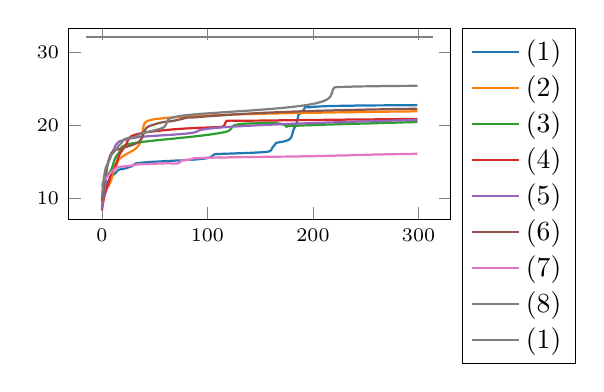
\begin{tikzpicture}

\definecolor{crimson2143940}{RGB}{214,39,40}
\definecolor{darkgray176}{RGB}{176,176,176}
\definecolor{darkorange25512714}{RGB}{255,127,14}
\definecolor{forestgreen4416044}{RGB}{44,160,44}
\definecolor{gray127}{RGB}{127,127,127}
\definecolor{mediumpurple148103189}{RGB}{148,103,189}
\definecolor{orchid227119194}{RGB}{227,119,194}
\definecolor{sienna1408675}{RGB}{140,86,75}
\definecolor{steelblue31119180}{RGB}{31,119,180}

\begin{axis}[compar, legend pos=outer north east]
\addplot [thick, steelblue31119180]
table {%
0 8.68000030517578
1 9.89999961853027
2 10.6599998474121
3 11.2799997329712
4 11.6899995803833
5 12
6 12.2600002288818
7 12.4799995422363
8 12.6899995803833
9 12.9099998474121
10 13.0600004196167
11 13.1700000762939
12 13.289999961853
13 13.4200000762939
14 13.5900001525879
15 13.7700004577637
16 13.8500003814697
17 13.8900003433228
19 13.9499998092651
20 13.9700002670288
22 14.0299997329712
23 14.0699996948242
25 14.1700000762939
26 14.210000038147
28 14.3100004196167
29 14.3800001144409
30 14.4899997711182
31 14.6400003433228
32 14.6999998092651
33 14.7299995422363
37 14.8100004196167
38 14.8199996948242
39 14.8400001525879
41 14.8599996566772
42 14.8800001144409
49 14.9499998092651
50 14.9499998092651
55 15
56 15
59 15.0299997329712
60 15.0299997329712
63 15.0600004196167
64 15.0600004196167
66 15.0799999237061
67 15.0799999237061
70 15.1099996566772
71 15.1099996566772
73 15.1300001144409
74 15.1300001144409
77 15.1599998474121
78 15.1599998474121
83 15.210000038147
84 15.210000038147
91 15.2799997329712
92 15.3000001907349
94 15.3199996948242
95 15.3400001525879
96 15.3500003814697
98 15.3900003433228
101 15.4799995422363
102 15.5299997329712
103 15.5900001525879
104 15.6700000762939
105 15.789999961853
106 15.9200000762939
107 15.9799995422363
109 16
110 16
111 16.0100002288818
112 16.0100002288818
114 16.0300006866455
115 16.0300006866455
116 16.0400009155273
117 16.0400009155273
118 16.0499992370605
119 16.0499992370605
120 16.0599994659424
121 16.0599994659424
122 16.0699996948242
123 16.0699996948242
124 16.0799999237061
125 16.0799999237061
127 16.1000003814697
128 16.1000003814697
129 16.1100006103516
130 16.1100006103516
131 16.1200008392334
132 16.1200008392334
133 16.1299991607666
134 16.1299991607666
135 16.1399993896484
136 16.1399993896484
137 16.1499996185303
138 16.1499996185303
139 16.1599998474121
140 16.1599998474121
142 16.1800003051758
143 16.1800003051758
145 16.2000007629395
146 16.2000007629395
149 16.2299995422363
150 16.2299995422363
154 16.2700004577637
155 16.2900009155273
156 16.2999992370605
157 16.3199996948242
158 16.3500003814697
159 16.3899993896484
160 16.4799995422363
161 16.7099990844727
162 17
163 17.1100006103516
164 17.2900009155273
165 17.5300006866455
166 17.5599994659424
167 17.5799999237061
168 17.6100006103516
169 17.6299991607666
170 17.6599998474121
171 17.6800003051758
172 17.7099990844727
175 17.8299999237061
176 17.8899993896484
177 17.9599990844727
178 18.0599994659424
179 18.2199993133545
180 18.5100002288818
181 19.0799999237061
182 19.5200004577637
183 19.7199993133545
184 20
185 20.4899997711182
186 21.2999992370605
187 21.4699993133545
188 21.5699996948242
189 21.6800003051758
190 21.8299999237061
191 22.0200004577637
192 22.2700004577637
193 22.5599994659424
194 22.5699996948242
195 22.3899993896484
196 22.3999996185303
197 22.4200000762939
198 22.4300003051758
199 22.4500007629395
207 22.5300006866455
208 22.5300006866455
210 22.5499992370605
211 22.5499992370605
212 22.5599994659424
213 22.5599994659424
214 22.5699996948242
215 22.5699996948242
216 22.5799999237061
218 22.5799999237061
219 22.5900001525879
221 22.5900001525879
222 22.6000003814697
225 22.6000003814697
226 22.6100006103516
229 22.6100006103516
230 22.6200008392334
233 22.6200008392334
234 22.6299991607666
239 22.6299991607666
240 22.6399993896484
245 22.6399993896484
246 22.6499996185303
251 22.6499996185303
252 22.6599998474121
259 22.6599998474121
260 22.6700000762939
267 22.6700000762939
268 22.6800003051758
276 22.6800003051758
277 22.6900005340576
286 22.6900005340576
287 22.7000007629395
297 22.7000007629395
298 22.7099990844727
299 22.7099990844727
};
\addlegendentry{$(1)$}
\addplot [thick, darkorange25512714]
table {%
0 9.68000030517578
1 10.539999961853
2 10.960000038147
3 11.1499996185303
4 11.289999961853
5 11.4099998474121
6 11.5500001907349
7 11.789999961853
8 12.1199998855591
9 12.4799995422363
11 13.6400003433228
12 14.0299997329712
13 14.25
14 14.5100002288818
15 14.9200000762939
16 15.2200002670288
17 15.3800001144409
18 15.5200004577637
19 15.6099996566772
20 15.6899995803833
21 15.7799997329712
23 15.9799995422363
25 16.1399993896484
26 16.2099990844727
29 16.4500007629395
30 16.5400009155273
31 16.6399993896484
32 16.75
33 16.8799991607666
34 17.0300006866455
35 17.2299995422363
36 17.5
37 17.9200000762939
38 18.6000003814697
39 19.4300003051758
40 20.1200008392334
41 20.3199996948242
42 20.4400005340576
43 20.5100002288818
44 20.5699996948242
45 20.6200008392334
46 20.6599998474121
48 20.7199993133545
49 20.7399997711182
50 20.7700004577637
54 20.8500003814697
55 20.8600006103516
57 20.8999996185303
59 20.9200000762939
60 20.9400005340576
63 20.9699993133545
64 20.9899997711182
73 21.0799999237061
74 21.0799999237061
79 21.1299991607666
80 21.1299991607666
83 21.1599998474121
84 21.1599998474121
87 21.1900005340576
88 21.1900005340576
90 21.2099990844727
91 21.2099990844727
93 21.2299995422363
94 21.2299995422363
96 21.25
97 21.25
99 21.2700004577637
100 21.2700004577637
102 21.2900009155273
103 21.2900009155273
105 21.3099994659424
106 21.3099994659424
107 21.3199996948242
108 21.3199996948242
110 21.3400001525879
111 21.3400001525879
112 21.3500003814697
113 21.3500003814697
115 21.3700008392334
116 21.3700008392334
117 21.3799991607666
118 21.3799991607666
119 21.3899993896484
120 21.3899993896484
121 21.3999996185303
122 21.3999996185303
123 21.4099998474121
124 21.4099998474121
125 21.4200000762939
126 21.4200000762939
127 21.4300003051758
128 21.4300003051758
129 21.4400005340576
131 21.4400005340576
132 21.4500007629395
133 21.4500007629395
134 21.4599990844727
135 21.4599990844727
136 21.4699993133545
138 21.4699993133545
139 21.4799995422363
140 21.4799995422363
141 21.4899997711182
143 21.4899997711182
144 21.5
146 21.5
147 21.5100002288818
149 21.5100002288818
150 21.5200004577637
152 21.5200004577637
153 21.5300006866455
155 21.5300006866455
156 21.5400009155273
158 21.5400009155273
159 21.5499992370605
161 21.5499992370605
162 21.5599994659424
164 21.5599994659424
165 21.5699996948242
168 21.5699996948242
169 21.5799999237061
171 21.5799999237061
172 21.5900001525879
175 21.5900001525879
176 21.6000003814697
179 21.6000003814697
180 21.6100006103516
182 21.6100006103516
183 21.6200008392334
186 21.6200008392334
187 21.6299991607666
190 21.6299991607666
191 21.6399993896484
195 21.6399993896484
196 21.6499996185303
199 21.6499996185303
200 21.6599998474121
203 21.6599998474121
204 21.6700000762939
208 21.6700000762939
209 21.6800003051758
212 21.6800003051758
213 21.6900005340576
217 21.6900005340576
218 21.7000007629395
221 21.7000007629395
222 21.7099990844727
226 21.7099990844727
227 21.7199993133545
231 21.7199993133545
232 21.7299995422363
236 21.7299995422363
237 21.7399997711182
241 21.7399997711182
242 21.75
246 21.75
247 21.7600002288818
251 21.7600002288818
252 21.7700004577637
256 21.7700004577637
257 21.7800006866455
261 21.7800006866455
262 21.7900009155273
266 21.7900009155273
267 21.7999992370605
271 21.7999992370605
272 21.8099994659424
276 21.8099994659424
277 21.8199996948242
282 21.8199996948242
283 21.8299999237061
287 21.8299999237061
288 21.8400001525879
292 21.8400001525879
293 21.8500003814697
297 21.8500003814697
298 21.8600006103516
299 21.8600006103516
};
\addlegendentry{$(2)$}
\addplot [thick, forestgreen4416044]
table {%
0 9.94999980926514
1 10.8699998855591
2 11.7399997711182
3 12.3800001144409
4 12.6800003051758
5 12.9300003051758
6 13.1499996185303
7 13.3999996185303
8 13.6099996566772
9 13.8999996185303
10 14.2799997329712
12 15.2200002670288
13 15.5500001907349
14 15.7600002288818
15 15.9399995803833
16 16.1399993896484
17 16.4099998474121
18 16.75
19 16.9899997711182
20 17.0699996948242
21 17.1399993896484
24 17.2900009155273
26 17.3700008392334
27 17.3999996185303
28 17.4400005340576
29 17.4699993133545
30 17.4899997711182
31 17.5200004577637
36 17.6200008392334
37 17.6299991607666
41 17.7099990844727
42 17.7199993133545
45 17.7800006866455
46 17.7900009155273
47 17.8099994659424
48 17.8199996948242
49 17.8400001525879
50 17.8500003814697
52 17.8899993896484
53 17.8999996185303
54 17.9200000762939
55 17.9300003051758
56 17.9500007629395
58 17.9699993133545
59 17.9899997711182
60 18
61 18.0200004577637
62 18.0300006866455
63 18.0499992370605
64 18.0599994659424
65 18.0799999237061
67 18.1000003814697
68 18.1200008392334
69 18.1299991607666
70 18.1499996185303
71 18.1599998474121
72 18.1800003051758
73 18.1900005340576
74 18.2099990844727
75 18.2199993133545
76 18.2399997711182
77 18.25
78 18.2700004577637
79 18.2800006866455
80 18.2999992370605
81 18.3099994659424
82 18.3299999237061
83 18.3400001525879
84 18.3600006103516
85 18.3700008392334
87 18.4099998474121
88 18.4200000762939
90 18.4599990844727
91 18.4699993133545
93 18.5100002288818
94 18.5200004577637
99 18.6200008392334
100 18.6299991607666
105 18.7299995422363
106 18.7600002288818
110 18.8400001525879
111 18.8700008392334
112 18.8899993896484
113 18.9200000762939
114 18.9400005340576
117 19.0300006866455
118 19.0699996948242
119 19.1200008392334
120 19.1800003051758
121 19.2700004577637
122 19.4099998474121
123 19.6299991607666
124 19.8099994659424
125 19.9099998474121
126 19.9699993133545
127 20.0100002288818
129 20.0699996948242
131 20.1100006103516
138 20.1800003051758
139 20.1800003051758
140 20.1900005340576
141 20.1900005340576
143 20.2099990844727
145 20.2099990844727
146 20.2199993133545
148 20.2199993133545
149 20.2299995422363
151 20.2299995422363
152 20.2399997711182
162 20.2399997711182
163 20.2299995422363
164 20.2299995422363
167 20.2000007629395
170 20.1399993896484
171 20.1000003814697
173 19.9799995422363
174 19.8899993896484
175 19.7199993133545
176 19.8199996948242
180 19.8600006103516
181 19.8600006103516
183 19.8799991607666
184 19.8799991607666
185 19.8899993896484
186 19.8899993896484
188 19.9099998474121
189 19.9099998474121
190 19.9200000762939
191 19.9200000762939
192 19.9300003051758
193 19.9300003051758
194 19.9400005340576
195 19.9400005340576
196 19.9500007629395
197 19.9500007629395
198 19.9599990844727
199 19.9599990844727
200 19.9699993133545
201 19.9699993133545
202 19.9799995422363
203 19.9799995422363
204 19.9899997711182
205 19.9899997711182
206 20
207 20
208 20.0100002288818
209 20.0100002288818
210 20.0200004577637
211 20.0200004577637
212 20.0300006866455
214 20.0300006866455
215 20.0400009155273
216 20.0400009155273
217 20.0499992370605
218 20.0499992370605
219 20.0599994659424
220 20.0599994659424
221 20.0699996948242
223 20.0699996948242
224 20.0799999237061
225 20.0799999237061
226 20.0900001525879
227 20.0900001525879
228 20.1000003814697
230 20.1000003814697
231 20.1100006103516
232 20.1100006103516
233 20.1200008392334
234 20.1200008392334
235 20.1299991607666
237 20.1299991607666
238 20.1399993896484
239 20.1399993896484
240 20.1499996185303
242 20.1499996185303
243 20.1599998474121
244 20.1599998474121
245 20.1700000762939
246 20.1700000762939
247 20.1800003051758
249 20.1800003051758
250 20.1900005340576
251 20.1900005340576
252 20.2000007629395
254 20.2000007629395
255 20.2099990844727
256 20.2099990844727
257 20.2199993133545
259 20.2199993133545
260 20.2299995422363
261 20.2299995422363
262 20.2399997711182
263 20.2399997711182
264 20.25
266 20.25
267 20.2600002288818
268 20.2600002288818
269 20.2700004577637
271 20.2700004577637
272 20.2800006866455
273 20.2800006866455
274 20.2900009155273
275 20.2900009155273
276 20.2999992370605
278 20.2999992370605
279 20.3099994659424
280 20.3099994659424
281 20.3199996948242
283 20.3199996948242
284 20.3299999237061
285 20.3299999237061
286 20.3400001525879
287 20.3400001525879
288 20.3500003814697
290 20.3500003814697
291 20.3600006103516
292 20.3600006103516
293 20.3700008392334
294 20.3700008392334
295 20.3799991607666
296 20.3799991607666
297 20.3899993896484
299 20.3899993896484
};
\addlegendentry{$(3)$}
\addplot [thick, crimson2143940]
table {%
0 8.27000045776367
1 9.25
3 10.5799999237061
4 11
5 11.5799999237061
6 11.9499998092651
7 12.3699998855591
8 12.9300003051758
9 13.3699998855591
10 13.6599998474121
11 13.8999996185303
12 14.1599998474121
13 14.5200004577637
14 14.8699998855591
16 15.710000038147
17 16.0300006866455
19 16.4699993133545
20 16.6700000762939
21 16.8799991607666
22 17.1000003814697
23 17.3500003814697
24 17.6299991607666
25 17.9599990844727
26 18.2299995422363
27 18.3600006103516
28 18.4400005340576
29 18.5100002288818
30 18.5699996948242
32 18.6700000762939
35 18.7900009155273
39 18.9099998474121
41 18.9500007629395
42 18.9799995422363
46 19.0599994659424
47 19.0699996948242
49 19.1100006103516
50 19.1200008392334
52 19.1599998474121
53 19.1700000762939
54 19.1900005340576
55 19.2000007629395
56 19.2199993133545
57 19.2299995422363
58 19.25
59 19.2600002288818
60 19.2800006866455
61 19.2900009155273
62 19.3099994659424
64 19.3299999237061
65 19.3500003814697
67 19.3700008392334
68 19.3899993896484
81 19.5200004577637
82 19.5200004577637
85 19.5499992370605
86 19.5499992370605
88 19.5699996948242
89 19.5699996948242
91 19.5900001525879
92 19.5900001525879
93 19.6000003814697
94 19.6000003814697
95 19.6100006103516
96 19.6100006103516
97 19.6200008392334
98 19.6200008392334
99 19.6299991607666
100 19.6299991607666
101 19.6399993896484
102 19.6399993896484
103 19.6499996185303
104 19.6499996185303
105 19.6599998474121
106 19.6599998474121
107 19.6700000762939
108 19.6700000762939
109 19.6800003051758
110 19.6800003051758
112 19.7000007629395
113 19.7199993133545
114 19.75
115 19.7999992370605
116 19.9400005340576
117 20.2800006866455
118 20.5200004577637
119 20.5499992370605
120 20.5699996948242
121 20.5699996948242
122 20.5799999237061
123 20.5799999237061
124 20.5699996948242
142 20.5699996948242
143 20.5799999237061
149 20.5799999237061
150 20.5900001525879
156 20.5900001525879
157 20.6000003814697
162 20.6000003814697
163 20.6100006103516
167 20.6100006103516
168 20.6200008392334
173 20.6200008392334
174 20.6299991607666
179 20.6299991607666
180 20.6399993896484
185 20.6399993896484
186 20.6499996185303
191 20.6499996185303
192 20.6599998474121
198 20.6599998474121
199 20.6700000762939
204 20.6700000762939
205 20.6800003051758
210 20.6800003051758
211 20.6900005340576
217 20.6900005340576
218 20.7000007629395
223 20.7000007629395
224 20.7099990844727
230 20.7099990844727
231 20.7199993133545
237 20.7199993133545
238 20.7299995422363
244 20.7299995422363
245 20.7399997711182
251 20.7399997711182
252 20.75
258 20.75
259 20.7600002288818
265 20.7600002288818
266 20.7700004577637
272 20.7700004577637
273 20.7800006866455
279 20.7800006866455
280 20.7900009155273
286 20.7900009155273
287 20.7999992370605
294 20.7999992370605
295 20.8099994659424
299 20.8099994659424
};
\addlegendentry{$(4)$}
\addplot [thick, mediumpurple148103189]
table {%
0 8.46000003814697
1 9.48999977111816
2 10.7399997711182
3 11.5
4 12.8900003433228
5 14.2299995422363
6 14.7799997329712
7 15.25
8 15.7600002288818
9 16.0599994659424
10 16.2999992370605
11 16.5499992370605
12 16.8799991607666
13 17.2000007629395
14 17.3999996185303
15 17.5699996948242
16 17.6900005340576
17 17.75
18 17.7999992370605
23 18
24 18.0300006866455
25 18.0699996948242
29 18.1900005340576
30 18.2099990844727
31 18.2399997711182
35 18.3199996948242
36 18.3299999237061
37 18.3500003814697
38 18.3600006103516
39 18.3799991607666
42 18.4099998474121
43 18.4300003051758
50 18.5
51 18.5
63 18.6200008392334
64 18.6200008392334
68 18.6599998474121
69 18.6800003051758
76 18.75
77 18.7700004577637
79 18.7900009155273
80 18.8099994659424
81 18.8199996948242
83 18.8600006103516
84 18.8700008392334
85 18.8899993896484
86 18.9200000762939
87 18.9400005340576
89 19.0200004577637
90 19.0799999237061
91 19.1599998474121
92 19.2299995422363
93 19.2900009155273
96 19.3799991607666
101 19.4799995422363
102 19.4899997711182
103 19.5100002288818
104 19.5200004577637
105 19.5400009155273
106 19.5499992370605
107 19.5699996948242
109 19.5900001525879
110 19.6100006103516
113 19.6399993896484
114 19.6599998474121
125 19.7700004577637
126 19.7700004577637
131 19.8199996948242
132 19.8199996948242
136 19.8600006103516
137 19.8600006103516
140 19.8899993896484
141 19.8899993896484
144 19.9200000762939
145 19.9200000762939
147 19.9400005340576
148 19.9400005340576
150 19.9599990844727
151 19.9599990844727
153 19.9799995422363
154 19.9799995422363
156 20
157 20
159 20.0200004577637
160 20.0200004577637
162 20.0400009155273
163 20.0400009155273
164 20.0499992370605
165 20.0499992370605
167 20.0699996948242
168 20.0699996948242
169 20.0799999237061
170 20.0799999237061
172 20.1000003814697
173 20.1000003814697
174 20.1100006103516
175 20.1100006103516
177 20.1299991607666
178 20.1299991607666
179 20.1399993896484
180 20.1399993896484
181 20.1499996185303
182 20.1499996185303
184 20.1700000762939
185 20.1700000762939
186 20.1800003051758
187 20.1800003051758
188 20.1900005340576
189 20.1900005340576
190 20.2000007629395
191 20.2000007629395
192 20.2099990844727
193 20.2099990844727
194 20.2199993133545
195 20.2199993133545
196 20.2299995422363
197 20.2299995422363
199 20.25
200 20.25
201 20.2600002288818
202 20.2600002288818
203 20.2700004577637
204 20.2700004577637
205 20.2800006866455
206 20.2800006866455
207 20.2900009155273
208 20.2900009155273
209 20.2999992370605
211 20.2999992370605
212 20.3099994659424
213 20.3099994659424
214 20.3199996948242
215 20.3199996948242
216 20.3299999237061
217 20.3299999237061
218 20.3400001525879
219 20.3400001525879
220 20.3500003814697
221 20.3500003814697
222 20.3600006103516
223 20.3600006103516
224 20.3700008392334
226 20.3700008392334
227 20.3799991607666
228 20.3799991607666
229 20.3899993896484
230 20.3899993896484
231 20.3999996185303
232 20.3999996185303
233 20.4099998474121
235 20.4099998474121
236 20.4200000762939
237 20.4200000762939
238 20.4300003051758
239 20.4300003051758
240 20.4400005340576
241 20.4400005340576
242 20.4500007629395
244 20.4500007629395
245 20.4599990844727
246 20.4599990844727
247 20.4699993133545
249 20.4699993133545
250 20.4799995422363
251 20.4799995422363
252 20.4899997711182
254 20.4899997711182
255 20.5
256 20.5
257 20.5100002288818
258 20.5100002288818
259 20.5200004577637
261 20.5200004577637
262 20.5300006866455
263 20.5300006866455
264 20.5400009155273
266 20.5400009155273
267 20.5499992370605
269 20.5499992370605
270 20.5599994659424
271 20.5599994659424
272 20.5699996948242
274 20.5699996948242
275 20.5799999237061
276 20.5799999237061
277 20.5900001525879
279 20.5900001525879
280 20.6000003814697
282 20.6000003814697
283 20.6100006103516
284 20.6100006103516
285 20.6200008392334
287 20.6200008392334
288 20.6299991607666
290 20.6299991607666
291 20.6399993896484
292 20.6399993896484
293 20.6499996185303
295 20.6499996185303
296 20.6599998474121
298 20.6599998474121
299 20.6700000762939
};
\addlegendentry{$(5)$}
\addplot [thick, sienna1408675]
table {%
0 9.52999973297119
1 10.4399995803833
2 11.7700004577637
3 13.039999961853
4 13.7799997329712
5 14.3900003433228
6 14.9399995803833
7 15.4099998474121
8 15.8000001907349
9 16.0699996948242
10 16.2600002288818
11 16.3899993896484
12 16.4899997711182
13 16.5499992370605
14 16.6000003814697
15 16.6299991607666
17 16.7099990844727
18 16.7600002288818
19 16.7999992370605
20 16.8500003814697
21 16.8899993896484
22 16.9400005340576
25 17.0599994659424
26 17.1100006103516
27 17.1499996185303
30 17.2999992370605
32 17.4200000762939
33 17.4899997711182
34 17.5699996948242
35 17.6700000762939
36 17.7999992370605
37 17.9799995422363
38 18.2299995422363
39 18.6200008392334
40 19.0699996948242
41 19.3500003814697
42 19.5300006866455
43 19.6599998474121
44 19.7600002288818
45 19.8299999237061
47 19.9300003051758
48 19.9699993133545
50 20.0699996948242
51 20.1100006103516
53 20.2099990844727
55 20.2900009155273
56 20.3199996948242
59 20.3799991607666
60 20.3899993896484
66 20.5100002288818
67 20.5400009155273
68 20.5599994659424
72 20.6800003051758
73 20.7199993133545
75 20.7800006866455
76 20.8199996948242
77 20.8500003814697
78 20.8899993896484
81 20.9799995422363
82 21
84 21.0200004577637
87 21.0200004577637
94 21.0900001525879
95 21.1100006103516
99 21.1499996185303
100 21.1700000762939
128 21.4500007629395
129 21.4500007629395
135 21.5100002288818
136 21.5100002288818
140 21.5499992370605
141 21.5499992370605
145 21.5900001525879
146 21.5900001525879
149 21.6200008392334
150 21.6200008392334
152 21.6399993896484
153 21.6399993896484
155 21.6599998474121
156 21.6599998474121
158 21.6800003051758
159 21.6800003051758
161 21.7000007629395
162 21.7000007629395
164 21.7199993133545
165 21.7199993133545
167 21.7399997711182
168 21.7399997711182
169 21.75
170 21.75
172 21.7700004577637
173 21.7700004577637
174 21.7800006866455
175 21.7800006866455
176 21.7900009155273
177 21.7900009155273
178 21.7999992370605
179 21.7999992370605
181 21.8199996948242
182 21.8199996948242
183 21.8299999237061
184 21.8299999237061
185 21.8400001525879
186 21.8400001525879
187 21.8500003814697
188 21.8500003814697
189 21.8600006103516
190 21.8600006103516
191 21.8700008392334
193 21.8700008392334
194 21.8799991607666
195 21.8799991607666
196 21.8899993896484
197 21.8899993896484
198 21.8999996185303
199 21.8999996185303
200 21.9099998474121
202 21.9099998474121
203 21.9200000762939
204 21.9200000762939
205 21.9300003051758
206 21.9300003051758
207 21.9400005340576
209 21.9400005340576
210 21.9500007629395
211 21.9500007629395
212 21.9599990844727
214 21.9599990844727
215 21.9699993133545
216 21.9699993133545
217 21.9799995422363
219 21.9799995422363
220 21.9899997711182
222 21.9899997711182
223 22
225 22
226 22.0100002288818
228 22.0100002288818
229 22.0200004577637
230 22.0200004577637
231 22.0300006866455
233 22.0300006866455
234 22.0400009155273
236 22.0400009155273
237 22.0499992370605
240 22.0499992370605
241 22.0599994659424
243 22.0599994659424
244 22.0699996948242
246 22.0699996948242
247 22.0799999237061
249 22.0799999237061
250 22.0900001525879
253 22.0900001525879
254 22.1000003814697
256 22.1000003814697
257 22.1100006103516
260 22.1100006103516
261 22.1200008392334
263 22.1200008392334
264 22.1299991607666
267 22.1299991607666
268 22.1399993896484
271 22.1399993896484
272 22.1499996185303
275 22.1499996185303
276 22.1599998474121
279 22.1599998474121
280 22.1700000762939
283 22.1700000762939
284 22.1800003051758
287 22.1800003051758
288 22.1900005340576
291 22.1900005340576
292 22.2000007629395
295 22.2000007629395
296 22.2099990844727
299 22.2099990844727
};
\addlegendentry{$(6)$}
\addplot [thick, orchid227119194]
table {%
0 11.5100002288818
1 12.1800003051758
2 12.3999996185303
3 12.5600004196167
4 12.7399997711182
5 12.8999996185303
6 13.0299997329712
7 13.1899995803833
8 13.3800001144409
9 13.539999961853
10 13.6800003051758
11 13.789999961853
12 13.9300003051758
13 14.1099996566772
14 14.1199998855591
15 14.210000038147
16 14.2200002670288
19 14.2799997329712
20 14.289999961853
21 14.3100004196167
22 14.3199996948242
23 14.3400001525879
24 14.3500003814697
29 14.4499998092651
31 14.5100002288818
32 14.5500001907349
33 14.5699996948242
35 14.5900001525879
36 14.5900001525879
38 14.6099996566772
39 14.6099996566772
40 14.6199998855591
41 14.6199998855591
43 14.6400003433228
44 14.6400003433228
45 14.6499996185303
46 14.6499996185303
47 14.6599998474121
48 14.6599998474121
49 14.6700000762939
50 14.6700000762939
51 14.6800003051758
52 14.6800003051758
53 14.6899995803833
54 14.6899995803833
56 14.710000038147
57 14.710000038147
58 14.7200002670288
59 14.7200002670288
60 14.7299995422363
64 14.7299995422363
66 14.710000038147
67 14.6899995803833
69 14.6899995803833
71 14.710000038147
72 14.7299995422363
73 14.7799997329712
74 14.8800001144409
75 15.0799999237061
76 15.1400003433228
78 15.1800003051758
83 15.2299995422363
84 15.25
85 15.3000001907349
86 15.3800001144409
87 15.4099998474121
91 15.4499998092651
92 15.4499998092651
93 15.460000038147
94 15.460000038147
95 15.4700002670288
96 15.4700002670288
97 15.4799995422363
99 15.4799995422363
100 15.4899997711182
101 15.4899997711182
102 15.5
104 15.5
105 15.5100002288818
107 15.5100002288818
108 15.5200004577637
111 15.5200004577637
112 15.5299997329712
114 15.5299997329712
115 15.539999961853
119 15.539999961853
120 15.5500001907349
123 15.5500001907349
124 15.5600004196167
127 15.5600004196167
128 15.5699996948242
132 15.5699996948242
133 15.5799999237061
137 15.5799999237061
138 15.5900001525879
142 15.5900001525879
143 15.6000003814697
148 15.6000003814697
149 15.6099996566772
153 15.6099996566772
154 15.6199998855591
158 15.6199998855591
159 15.6300001144409
164 15.6300001144409
165 15.6400003433228
169 15.6400003433228
170 15.6499996185303
174 15.6499996185303
175 15.6599998474121
179 15.6599998474121
180 15.6700000762939
184 15.6700000762939
185 15.6800003051758
188 15.6800003051758
189 15.6899995803833
193 15.6899995803833
194 15.6999998092651
197 15.6999998092651
198 15.710000038147
200 15.710000038147
201 15.7200002670288
204 15.7200002670288
205 15.7299995422363
207 15.7299995422363
208 15.7399997711182
210 15.7399997711182
211 15.75
213 15.75
214 15.7600002288818
216 15.7600002288818
217 15.7700004577637
219 15.7700004577637
220 15.7799997329712
221 15.7799997329712
222 15.789999961853
230 15.789999961853
234 15.8299999237061
235 15.8299999237061
237 15.8500003814697
238 15.8500003814697
239 15.8599996566772
240 15.8599996566772
241 15.8699998855591
243 15.8699998855591
244 15.8800001144409
245 15.8800001144409
246 15.8900003433228
248 15.8900003433228
249 15.8999996185303
250 15.8999996185303
251 15.9099998474121
253 15.9099998474121
254 15.9200000762939
256 15.9200000762939
257 15.9300003051758
260 15.9300003051758
261 15.9399995803833
263 15.9399995803833
264 15.9499998092651
266 15.9499998092651
267 15.960000038147
270 15.960000038147
271 15.9700002670288
274 15.9700002670288
275 15.9799995422363
278 15.9799995422363
279 15.9899997711182
282 15.9899997711182
283 16
286 16
287 16.0100002288818
290 16.0100002288818
291 16.0200004577637
294 16.0200004577637
295 16.0300006866455
299 16.0300006866455
};
\addlegendentry{$(7)$}
\addplot [thick, gray127]
table {%
0 10.0299997329712
1 11.4300003051758
2 12.8699998855591
3 13.7200002670288
4 14.2799997329712
5 14.5299997329712
6 14.8000001907349
7 15.1599998474121
8 15.4700002670288
9 15.8400001525879
10 16.0499992370605
12 16.3700008392334
13 16.5400009155273
14 16.7399997711182
15 16.9599990844727
16 17.1499996185303
18 17.4500007629395
19 17.6100006103516
21 17.9899997711182
22 18.0799999237061
23 18.1200008392334
26 18.2099990844727
27 18.2299995422363
28 18.2600002288818
29 18.2800006866455
32 18.3700008392334
33 18.4300003051758
34 18.5200004577637
35 18.6599998474121
36 18.7299995422363
37 18.7900009155273
38 18.8400001525879
41 18.9599990844727
42 18.9899997711182
43 19.0300006866455
46 19.1200008392334
47 19.1599998474121
49 19.2199993133545
50 19.2600002288818
51 19.2900009155273
55 19.4500007629395
56 19.5
58 19.6200008392334
59 19.7099990844727
60 19.8600006103516
61 20.1299991607666
62 20.5499992370605
63 20.7600002288818
64 20.8400001525879
65 20.9099998474121
66 20.9599990844727
69 21.0799999237061
71 21.1399993896484
72 21.1599998474121
73 21.1900005340576
79 21.3099994659424
80 21.3199996948242
81 21.3400001525879
82 21.3500003814697
83 21.3700008392334
84 21.3799991607666
85 21.3999996185303
87 21.4200000762939
88 21.4400005340576
92 21.4799995422363
93 21.5
129 21.8600006103516
130 21.8600006103516
146 22.0200004577637
147 22.0400009155273
156 22.1299991607666
157 22.1499996185303
162 22.2000007629395
163 22.2199993133545
166 22.25
167 22.2700004577637
169 22.2900009155273
170 22.3099994659424
172 22.3299999237061
173 22.3500003814697
174 22.3600006103516
175 22.3799991607666
176 22.3899993896484
177 22.4099998474121
178 22.4200000762939
179 22.4400005340576
180 22.4500007629395
182 22.4899997711182
183 22.5
187 22.5799999237061
188 22.5900001525879
191 22.6499996185303
192 22.6800003051758
195 22.7399997711182
196 22.7700004577637
197 22.7900009155273
199 22.8500003814697
200 22.8700008392334
202 22.9300003051758
203 22.9699993133545
204 23
208 23.1599998474121
210 23.2600002288818
211 23.3199996948242
213 23.4599990844727
214 23.5499992370605
215 23.6599998474121
216 23.8099994659424
217 24.0200004577637
218 24.3700008392334
219 24.8600006103516
220 25.0900001525879
221 25.1399993896484
222 25.1599998474121
223 25.1700000762939
224 25.1700000762939
226 25.1900005340576
227 25.1900005340576
228 25.2000007629395
229 25.2000007629395
230 25.2099990844727
231 25.2099990844727
232 25.2199993133545
234 25.2199993133545
235 25.2299995422363
236 25.2299995422363
237 25.2399997711182
239 25.2399997711182
240 25.25
242 25.25
243 25.2600002288818
246 25.2600002288818
247 25.2700004577637
250 25.2700004577637
251 25.2800006866455
254 25.2800006866455
255 25.2900009155273
258 25.2900009155273
259 25.2999992370605
263 25.2999992370605
264 25.3099994659424
269 25.3099994659424
270 25.3199996948242
275 25.3199996948242
276 25.3299999237061
282 25.3299999237061
283 25.3400001525879
289 25.3400001525879
290 25.3500003814697
298 25.3500003814697
299 25.3600006103516
};
\addlegendentry{$(8)$}
\addplot [thick, gray]
table {%
-14.95 32.0471801757813
313.95 32.0471801757813
};
\addlegendentry{$(1)$}
\end{axis}

\end{tikzpicture}
}
\end{tabular}
	%\caption{Plein de descentes --- sans passe-bas}
	%\label{fig:LGDunif-s}
%\end{figure}
%\begin{figure}[H]\centering
	%\begin{tabular}{c c c c c c c c}
$(1)$  &  $(2)$  &  $(3)$  &  $(4)$  &  $(5)$  &  $(6)$  &  $(7)$  &  $(8)$
	
\\

\includegraphics[width=0.1\textwidth]{resultats/LGD/multitarget/unif_1-init-pas=0.25_filtre=g-0.6}
&
\includegraphics[width=0.1\textwidth]{resultats/LGD/multitarget/unif_2-init-pas=0.25_filtre=g-0.6}
&
\includegraphics[width=0.1\textwidth]{resultats/LGD/multitarget/unif_3-init-pas=0.25_filtre=g-0.6}
&
\includegraphics[width=0.1\textwidth]{resultats/LGD/multitarget/unif_4-init-pas=0.25_filtre=g-0.6}
&
\includegraphics[width=0.1\textwidth]{resultats/LGD/multitarget/unif_5-init-pas=0.25_filtre=g-0.6}
&
\includegraphics[width=0.1\textwidth]{resultats/LGD/multitarget/unif_6-init-pas=0.25_filtre=g-0.6}
&
\includegraphics[width=0.1\textwidth]{resultats/LGD/multitarget/unif_7-init-pas=0.25_filtre=g-0.6}
&
\includegraphics[width=0.1\textwidth]{resultats/LGD/multitarget/unif_8-init-pas=0.25_filtre=g-0.6}

\\

\includegraphics[width=0.1\textwidth]{resultats/LGD/multitarget/unif_1-guess-pas=0.25_filtre=g-0.6}
&
\includegraphics[width=0.1\textwidth]{resultats/LGD/multitarget/unif_2-guess-pas=0.25_filtre=g-0.6}
&
\includegraphics[width=0.1\textwidth]{resultats/LGD/multitarget/unif_3-guess-pas=0.25_filtre=g-0.6}
&
\includegraphics[width=0.1\textwidth]{resultats/LGD/multitarget/unif_4-guess-pas=0.25_filtre=g-0.6}
&
\includegraphics[width=0.1\textwidth]{resultats/LGD/multitarget/unif_5-guess-pas=0.25_filtre=g-0.6}
&
\includegraphics[width=0.1\textwidth]{resultats/LGD/multitarget/unif_6-guess-pas=0.25_filtre=g-0.6}
&
\includegraphics[width=0.1\textwidth]{resultats/LGD/multitarget/unif_7-guess-pas=0.25_filtre=g-0.6}
&
\includegraphics[width=0.1\textwidth]{resultats/LGD/multitarget/unif_8-guess-pas=0.25_filtre=g-0.6}

\\

\includegraphics[width=0.1\textwidth]{resultats/LGD/multitarget/unif_1-target-pas=0.25_filtre=g-0.6}
&
\includegraphics[width=0.1\textwidth]{resultats/LGD/multitarget/unif_2-target-pas=0.25_filtre=g-0.6}
&
\includegraphics[width=0.1\textwidth]{resultats/LGD/multitarget/unif_3-target-pas=0.25_filtre=g-0.6}
&
\includegraphics[width=0.1\textwidth]{resultats/LGD/multitarget/unif_4-target-pas=0.25_filtre=g-0.6}
&
\includegraphics[width=0.1\textwidth]{resultats/LGD/multitarget/unif_5-target-pas=0.25_filtre=g-0.6}
&
\includegraphics[width=0.1\textwidth]{resultats/LGD/multitarget/unif_6-target-pas=0.25_filtre=g-0.6}
&
\includegraphics[width=0.1\textwidth]{resultats/LGD/multitarget/unif_7-target-pas=0.25_filtre=g-0.6}
&
\includegraphics[width=0.1\textwidth]{resultats/LGD/multitarget/unif_8-target-pas=0.25_filtre=g-0.6}

\\ \\



\multicolumn{2}{c}{Loss}  &  \multicolumn{4}{c}{PSNR{\color{white}bbbb}}

\\

\multicolumn{2}{c}{% This file was created with tikzplotlib v0.10.1.
\begin{tikzpicture}

\definecolor{crimson2143940}{RGB}{214,39,40}
\definecolor{darkgray176}{RGB}{176,176,176}
\definecolor{darkorange25512714}{RGB}{255,127,14}
\definecolor{forestgreen4416044}{RGB}{44,160,44}
\definecolor{gray127}{RGB}{127,127,127}
\definecolor{mediumpurple148103189}{RGB}{148,103,189}
\definecolor{orchid227119194}{RGB}{227,119,194}
\definecolor{sienna1408675}{RGB}{140,86,75}
\definecolor{steelblue31119180}{RGB}{31,119,180}

\begin{axis}[
height=\figheight,
tick align=outside,
tick pos=left,
width=\figwidth,
x grid style={darkgray176},
xmin=-14.95, xmax=313.95,
xtick style={color=black},
y grid style={darkgray176},
ymin=-0.137931874766946, ymax=4.29107548184693,
ytick style={color=black}
]
\addplot [semithick, steelblue31119180]
table {%
0 4.08975696563721
1 3.33637833595276
2 2.73532152175903
3 2.14240837097168
4 1.73033332824707
5 1.41092455387115
6 1.16093754768372
7 0.991315722465515
8 0.860567331314087
9 0.725079298019409
10 0.599795460700989
11 0.511585831642151
12 0.459132432937622
13 0.424915790557861
14 0.400811910629272
15 0.382651805877686
16 0.368227362632751
17 0.356281042098999
19 0.337035298347473
21 0.321447491645813
24 0.301400303840637
36 0.227512717247009
39 0.214333415031433
42 0.204669713973999
46 0.195551514625549
51 0.187734842300415
58 0.180206418037415
68 0.172708511352539
83 0.16473913192749
107 0.155456066131592
157 0.139991283416748
234 0.115403294563293
291 0.0978024005889893
299 0.0958188772201538
};
\addplot [semithick, darkorange25512714]
table {%
0 3.26711583137512
1 2.14453959465027
2 1.54826188087463
3 1.17449641227722
4 0.960880637168884
5 0.822623014450073
6 0.728369951248169
7 0.657516002655029
8 0.598540782928467
9 0.545978665351868
10 0.49743926525116
11 0.452995777130127
12 0.41500985622406
13 0.38573169708252
14 0.364342212677002
15 0.34827733039856
16 0.335496068000793
18 0.315586090087891
20 0.300094604492188
22 0.287321805953979
25 0.271495699882507
29 0.254361271858215
34 0.236733317375183
40 0.218833088874817
47 0.201139569282532
54 0.186703205108643
62 0.173661708831787
72 0.160796999931335
85 0.147242188453674
101 0.133771300315857
120 0.121079564094543
145 0.10771107673645
173 0.0958435535430908
205 0.0854647159576416
244 0.0760577917098999
291 0.0679656267166138
299 0.0668560266494751
};
\addplot [semithick, forestgreen4416044]
table {%
0 3.58641195297241
1 2.6538405418396
2 2.13788032531738
3 1.78784930706024
4 1.37945985794067
5 1.12811803817749
6 0.98441481590271
8 0.854376316070557
9 0.77478814125061
10 0.643280267715454
11 0.576423406600952
12 0.517259955406189
13 0.482311010360718
14 0.453768014907837
15 0.431882500648499
16 0.41350519657135
17 0.397852182388306
18 0.384169340133667
20 0.361188530921936
22 0.342472314834595
24 0.326731443405151
27 0.306684970855713
41 0.222695469856262
44 0.208269715309143
47 0.196796894073486
51 0.184648871421814
56 0.173093914985657
62 0.162851810455322
69 0.154046177864075
79 0.144849300384521
93 0.135518074035645
112 0.12615704536438
139 0.11614465713501
175 0.106065511703491
221 0.096435546875
279 0.0875242948532104
299 0.0850281715393066
};
\addplot [semithick, crimson2143940]
table {%
0 3.59980320930481
1 2.85580730438232
2 2.25819754600525
3 1.79236423969269
4 1.4870867729187
5 1.23685133457184
6 1.01497256755829
7 0.834818959236145
8 0.701505064964294
9 0.617039680480957
10 0.557190418243408
11 0.512237071990967
12 0.4766606092453
13 0.44723653793335
14 0.422152161598206
15 0.400389909744263
16 0.38130247592926
17 0.364439725875854
18 0.349431753158569
20 0.323838829994202
22 0.302755117416382
24 0.285131812095642
26 0.270244598388672
29 0.251532554626465
33 0.230435848236084
37 0.211970210075378
41 0.196309804916382
45 0.183892130851746
50 0.1722412109375
56 0.162061929702759
63 0.153334617614746
73 0.144187450408936
87 0.134868502616882
106 0.125523567199707
133 0.115573287010193
169 0.105540037155151
216 0.0956368446350098
275 0.0864048004150391
299 0.0833859443664551
};
\addplot [semithick, mediumpurple148103189]
table {%
0 3.77583575248718
1 2.80040860176086
2 2.06100153923035
3 1.67373323440552
4 1.40151214599609
5 1.19340789318085
6 1.02040004730225
8 0.643000960350037
9 0.547231912612915
10 0.501989364624023
11 0.472496509552002
12 0.450330257415771
13 0.43235981464386
14 0.417077898979187
16 0.391552448272705
18 0.370209455490112
20 0.351549386978149
23 0.326914072036743
27 0.297568202018738
31 0.270411372184753
34 0.252612829208374
37 0.238190770149231
40 0.226767897605896
44 0.214648723602295
49 0.202553629875183
56 0.189156770706177
64 0.177186012268066
74 0.165547847747803
86 0.154767632484436
101 0.144400715827942
120 0.134394407272339
144 0.124900341033936
175 0.115900635719299
214 0.107794165611267
266 0.100237846374512
299 0.0966178178787231
};
\addplot [semithick, sienna1408675]
table {%
0 3.66736721992493
1 3.04063200950623
2 2.61433243751526
3 2.23785066604614
4 1.98633766174316
5 1.82387554645538
6 1.64216637611389
7 1.47709512710571
8 1.34406971931458
9 1.15304672718048
10 0.947600126266479
11 0.748635053634644
12 0.600256681442261
13 0.531451940536499
14 0.483613252639771
15 0.447154402732849
16 0.41832709312439
17 0.394673466682434
18 0.374488592147827
19 0.35672926902771
21 0.326258420944214
23 0.300604581832886
25 0.278540849685669
27 0.25935161113739
29 0.24254834651947
32 0.22106409072876
35 0.203329801559448
38 0.188740491867065
41 0.176756978034973
45 0.163975238800049
50 0.151768088340759
56 0.140838861465454
63 0.131322026252747
72 0.122157573699951
84 0.113049268722534
100 0.104035019874573
122 0.094921350479126
151 0.0861783027648926
190 0.0777146816253662
242 0.0697096586227417
299 0.0633866786956787
};
\addplot [semithick, orchid227119194]
table {%
0 3.10344982147217
1 2.18883633613586
2 1.92422163486481
3 1.71474027633667
4 1.5747389793396
5 1.41690707206726
6 1.28026342391968
7 1.17937529087067
9 0.998045086860657
10 0.913097620010376
12 0.762445569038391
13 0.684967279434204
14 0.613244771957397
15 0.550602197647095
16 0.502213001251221
17 0.466002941131592
18 0.437830328941345
19 0.414852380752563
20 0.395334124565125
21 0.378178477287292
23 0.348371863365173
25 0.32202935218811
28 0.285735368728638
30 0.263975381851196
32 0.245723009109497
34 0.231244087219238
36 0.219715714454651
39 0.206244111061096
42 0.195900321006775
46 0.185289978981018
51 0.175272703170776
58 0.164806485176086
67 0.154733061790466
79 0.144463300704956
96 0.133213043212891
119 0.121365666389465
148 0.109667539596558
184 0.098354697227478
228 0.0877712965011597
281 0.0782246589660645
299 0.0755660533905029
};
\addplot [semithick, gray127]
table {%
0 3.63611721992493
1 2.41480541229248
2 1.53092908859253
3 1.11500060558319
4 0.889492154121399
5 0.691224336624146
6 0.566917657852173
7 0.479475259780884
8 0.413059592247009
9 0.364131331443787
10 0.328145146369934
11 0.300734043121338
12 0.279045343399048
13 0.261374950408936
14 0.246655106544495
15 0.234177708625793
17 0.214131593704224
19 0.198731899261475
21 0.186552762985229
24 0.172412276268005
27 0.161569476127625
31 0.150346517562866
36 0.139622449874878
42 0.129886627197266
50 0.120374202728271
60 0.11198353767395
73 0.104402661323547
92 0.0967868566513062
119 0.0892927646636963
160 0.0812585353851318
220 0.0728050470352173
299 0.064693808555603
};
\end{axis}

\end{tikzpicture}
}
&
\multicolumn{4}{c}{% This file was created with tikzplotlib v0.10.1.
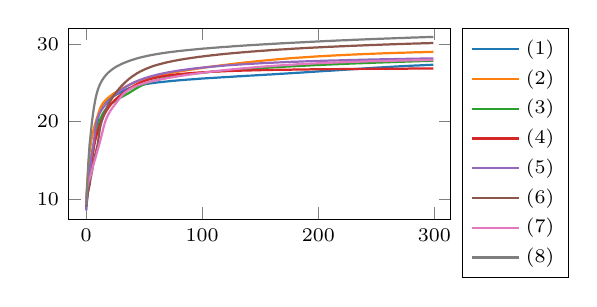
\begin{tikzpicture}

\definecolor{crimson2143940}{RGB}{214,39,40}
\definecolor{darkgray176}{RGB}{176,176,176}
\definecolor{darkorange25512714}{RGB}{255,127,14}
\definecolor{forestgreen4416044}{RGB}{44,160,44}
\definecolor{gray127}{RGB}{127,127,127}
\definecolor{mediumpurple148103189}{RGB}{148,103,189}
\definecolor{orchid227119194}{RGB}{227,119,194}
\definecolor{sienna1408675}{RGB}{140,86,75}
\definecolor{steelblue31119180}{RGB}{31,119,180}

\begin{axis}[compar, legend pos=outer north east]
\addplot [thick, steelblue31119180]
table {%
0 8.60000038146973
1 10.2700004577637
2 11.4200000762939
3 13.0299997329712
4 13.8900003433228
5 15.3999996185303
6 16.1200008392334
7 17.3600006103516
8 18.1200008392334
9 19.1800003051758
10 20.1299991607666
11 20.9400005340576
12 21.4799995422363
13 21.8500003814697
14 22.1200008392334
15 22.3299999237061
16 22.5
17 22.6499996185303
18 22.7700004577637
19 22.8799991607666
20 22.9799995422363
21 23.0699996948242
26 23.4699993133545
27 23.5400009155273
29 23.7000007629395
30 23.7700004577637
33 24.0100002288818
36 24.2199993133545
38 24.3400001525879
41 24.4899997711182
44 24.6100006103516
45 24.6399993896484
46 24.6800003051758
48 24.7399997711182
49 24.7600002288818
51 24.8199996948242
53 24.8600006103516
54 24.8899993896484
62 25.0499992370605
63 25.0599994659424
65 25.1000003814697
66 25.1100006103516
67 25.1299991607666
68 25.1399993896484
69 25.1599998474121
70 25.1700000762939
71 25.1900005340576
72 25.2000007629395
73 25.2199993133545
74 25.2299995422363
75 25.25
77 25.2700004577637
78 25.2900009155273
81 25.3199996948242
82 25.3400001525879
86 25.3799991607666
87 25.3999996185303
96 25.4899997711182
97 25.5100002288818
108 25.6200008392334
109 25.6200008392334
122 25.75
123 25.75
132 25.8400001525879
133 25.8400001525879
141 25.9200000762939
142 25.9200000762939
149 25.9899997711182
150 25.9899997711182
158 26.0699996948242
159 26.0699996948242
168 26.1599998474121
169 26.1599998474121
181 26.2800006866455
182 26.2800006866455
208 26.5400009155273
209 26.5400009155273
251 26.9599990844727
252 26.9599990844727
260 27.0400009155273
261 27.0400009155273
267 27.1000003814697
268 27.1000003814697
272 27.1399993896484
273 27.1399993896484
276 27.1700000762939
277 27.1700000762939
280 27.2000007629395
281 27.2000007629395
283 27.2199993133545
284 27.2199993133545
286 27.2399997711182
287 27.2399997711182
289 27.2600002288818
290 27.2600002288818
292 27.2800006866455
293 27.2800006866455
295 27.2999992370605
296 27.2999992370605
297 27.3099994659424
298 27.3099994659424
299 27.3199996948242
};
\addlegendentry{\scriptsize{$(1)$}}
\addplot [thick, darkorange25512714]
table {%
0 9.44999980926514
1 12.2700004577637
2 14.0500001907349
3 15.9799995422363
4 17.0699996948242
5 17.9899997711182
6 18.7000007629395
7 19.2800006866455
8 19.7900009155273
9 20.2800006866455
11 21.2199993133545
12 21.6299991607666
13 21.9699993133545
14 22.2399997711182
15 22.4500007629395
16 22.6299991607666
17 22.7900009155273
18 22.9300003051758
19 23.0599994659424
21 23.2999992370605
23 23.5200004577637
25 23.7199993133545
30 24.1700000762939
34 24.4899997711182
36 24.6299991607666
37 24.7099990844727
38 24.7800006866455
39 24.8400001525879
40 24.9099998474121
41 24.9699993133545
42 25.0400009155273
44 25.1599998474121
45 25.2099990844727
46 25.2700004577637
51 25.5200004577637
52 25.5599994659424
53 25.6100006103516
57 25.7700004577637
58 25.7999992370605
59 25.8400001525879
60 25.8700008392334
61 25.9099998474121
64 26
65 26.0400009155273
67 26.1000003814697
68 26.1200008392334
72 26.2399997711182
73 26.2600002288818
75 26.3199996948242
76 26.3400001525879
77 26.3700008392334
78 26.3899993896484
80 26.4500007629395
81 26.4699993133545
82 26.5
84 26.5400009155273
85 26.5699996948242
86 26.5900001525879
87 26.6200008392334
89 26.6599998474121
90 26.6900005340576
92 26.7299995422363
93 26.7600002288818
95 26.7999992370605
96 26.8299999237061
101 26.9300003051758
102 26.9599990844727
119 27.2999992370605
120 27.3099994659424
125 27.4099998474121
126 27.4200000762939
129 27.4799995422363
130 27.4899997711182
133 27.5499992370605
134 27.5599994659424
136 27.6000003814697
137 27.6100006103516
139 27.6499996185303
140 27.6599998474121
141 27.6800003051758
142 27.6900005340576
144 27.7299995422363
145 27.7399997711182
146 27.7600002288818
147 27.7700004577637
148 27.7900009155273
149 27.7999992370605
150 27.8199996948242
151 27.8299999237061
152 27.8500003814697
153 27.8600006103516
154 27.8799991607666
155 27.8899993896484
156 27.9099998474121
158 27.9300003051758
159 27.9500007629395
160 27.9599990844727
161 27.9799995422363
163 28
164 28.0200004577637
167 28.0499992370605
168 28.0699996948242
171 28.1000003814697
172 28.1200008392334
176 28.1599998474121
177 28.1800003051758
202 28.4300003051758
203 28.4300003051758
209 28.4899997711182
210 28.4899997711182
213 28.5200004577637
214 28.5200004577637
218 28.5599994659424
219 28.5599994659424
221 28.5799999237061
222 28.5799999237061
225 28.6100006103516
226 28.6100006103516
228 28.6299991607666
229 28.6299991607666
231 28.6499996185303
232 28.6499996185303
234 28.6700000762939
235 28.6700000762939
237 28.6900005340576
238 28.6900005340576
239 28.7000007629395
240 28.7000007629395
242 28.7199993133545
243 28.7199993133545
244 28.7299995422363
245 28.7299995422363
247 28.75
248 28.75
249 28.7600002288818
250 28.7600002288818
251 28.7700004577637
252 28.7700004577637
253 28.7800006866455
254 28.7800006866455
256 28.7999992370605
257 28.7999992370605
258 28.8099994659424
259 28.8099994659424
260 28.8199996948242
261 28.8199996948242
262 28.8299999237061
263 28.8299999237061
264 28.8400001525879
265 28.8400001525879
266 28.8500003814697
267 28.8500003814697
268 28.8600006103516
269 28.8600006103516
270 28.8700008392334
271 28.8700008392334
272 28.8799991607666
274 28.8799991607666
275 28.8899993896484
276 28.8899993896484
277 28.8999996185303
278 28.8999996185303
279 28.9099998474121
280 28.9099998474121
281 28.9200000762939
282 28.9200000762939
283 28.9300003051758
285 28.9300003051758
286 28.9400005340576
287 28.9400005340576
288 28.9500007629395
290 28.9500007629395
291 28.9599990844727
292 28.9599990844727
293 28.9699993133545
295 28.9699993133545
296 28.9799995422363
297 28.9799995422363
298 28.9899997711182
299 28.9899997711182
};
\addlegendentry{\scriptsize{$(2)$}}
\addplot [thick, forestgreen4416044]
table {%
0 9.02999973297119
1 10.9499998092651
2 12.0699996948242
3 13.0100002288818
4 14.5299997329712
5 15.7600002288818
6 16.7700004577637
7 17.2199993133545
8 17.9200000762939
9 18.3600006103516
10 19.3099994659424
11 19.7099990844727
12 20.2600002288818
13 20.5499992370605
14 20.8999996185303
15 21.1299991607666
16 21.3799991607666
17 21.5599994659424
18 21.75
19 21.9099998474121
20 22.0599994659424
21 22.2000007629395
23 22.4400005340576
24 22.5499992370605
27 22.8500003814697
28 22.9400005340576
29 23.0200004577637
30 23.1100006103516
33 23.3500003814697
34 23.4400005340576
36 23.6000003814697
38 23.7800006866455
39 23.8799991607666
41 24.0599994659424
42 24.1599998474121
43 24.25
44 24.3299999237061
45 24.4200000762939
47 24.5799999237061
51 24.8600006103516
54 25.0400009155273
58 25.2399997711182
60 25.3199996948242
61 25.3700008392334
62 25.3999996185303
64 25.4799995422363
65 25.5100002288818
66 25.5499992370605
73 25.7600002288818
74 25.7800006866455
75 25.8099994659424
76 25.8299999237061
77 25.8600006103516
79 25.8999996185303
80 25.9300003051758
90 26.1299991607666
91 26.1399993896484
94 26.2000007629395
95 26.2099990844727
97 26.25
98 26.2600002288818
99 26.2800006866455
100 26.2900009155273
101 26.3099994659424
102 26.3199996948242
103 26.3400001525879
104 26.3500003814697
105 26.3700008392334
106 26.3799991607666
107 26.3999996185303
109 26.4200000762939
110 26.4400005340576
112 26.4599990844727
113 26.4799995422363
116 26.5100002288818
117 26.5300006866455
120 26.5599994659424
121 26.5799999237061
125 26.6200008392334
126 26.6399993896484
136 26.7399997711182
137 26.7600002288818
148 26.8700008392334
149 26.8700008392334
160 26.9799995422363
161 26.9799995422363
167 27.0400009155273
168 27.0400009155273
173 27.0900001525879
174 27.0900001525879
178 27.1299991607666
179 27.1299991607666
183 27.1700000762939
184 27.1700000762939
187 27.2000007629395
188 27.2000007629395
190 27.2199993133545
191 27.2199993133545
194 27.25
195 27.25
198 27.2800006866455
199 27.2800006866455
201 27.2999992370605
202 27.2999992370605
204 27.3199996948242
205 27.3199996948242
207 27.3400001525879
208 27.3400001525879
210 27.3600006103516
211 27.3600006103516
213 27.3799991607666
214 27.3799991607666
216 27.3999996185303
217 27.3999996185303
219 27.4200000762939
220 27.4200000762939
221 27.4300003051758
222 27.4300003051758
224 27.4500007629395
225 27.4500007629395
227 27.4699993133545
228 27.4699993133545
229 27.4799995422363
230 27.4799995422363
232 27.5
233 27.5
234 27.5100002288818
235 27.5100002288818
236 27.5200004577637
237 27.5200004577637
239 27.5400009155273
240 27.5400009155273
241 27.5499992370605
242 27.5499992370605
243 27.5599994659424
244 27.5599994659424
246 27.5799999237061
247 27.5799999237061
248 27.5900001525879
249 27.5900001525879
250 27.6000003814697
251 27.6000003814697
252 27.6100006103516
253 27.6100006103516
254 27.6200008392334
255 27.6200008392334
257 27.6399993896484
258 27.6399993896484
259 27.6499996185303
260 27.6499996185303
261 27.6599998474121
262 27.6599998474121
263 27.6700000762939
264 27.6700000762939
265 27.6800003051758
266 27.6800003051758
267 27.6900005340576
268 27.6900005340576
269 27.7000007629395
270 27.7000007629395
271 27.7099990844727
272 27.7099990844727
273 27.7199993133545
274 27.7199993133545
275 27.7299995422363
276 27.7299995422363
277 27.7399997711182
278 27.7399997711182
279 27.75
280 27.75
281 27.7600002288818
282 27.7600002288818
283 27.7700004577637
285 27.7700004577637
286 27.7800006866455
287 27.7800006866455
288 27.7900009155273
289 27.7900009155273
290 27.7999992370605
291 27.7999992370605
292 27.8099994659424
293 27.8099994659424
294 27.8199996948242
296 27.8199996948242
297 27.8299999237061
298 27.8299999237061
299 27.8400001525879
};
\addlegendentry{\scriptsize{$(3)$}}
\addplot [thick, crimson2143940]
table {%
0 9.06999969482422
1 10.2600002288818
2 11.5900001525879
3 12.8900003433228
4 14.0600004196167
5 14.9799995422363
6 15.9899997711182
7 16.9200000762939
8 17.6499996185303
9 18.2299995422363
10 18.75
11 19.2099990844727
12 19.6200008392334
13 20
14 20.3600006103516
15 20.6800003051758
16 20.9799995422363
17 21.25
18 21.5100002288818
20 21.9500007629395
22 22.3299999237061
24 22.6499996185303
25 22.7900009155273
26 22.9400005340576
28 23.2000007629395
29 23.3099994659424
30 23.4400005340576
35 23.9899997711182
40 24.4899997711182
41 24.5799999237061
42 24.6599998474121
43 24.75
44 24.8199996948242
45 24.8999996185303
47 25.0400009155273
50 25.2199993133545
54 25.4200000762939
59 25.6200008392334
62 25.7099990844727
63 25.75
64 25.7700004577637
66 25.8299999237061
67 25.8500003814697
68 25.8799991607666
70 25.9200000762939
71 25.9500007629395
75 26.0300006866455
76 26.0400009155273
79 26.1000003814697
80 26.1100006103516
81 26.1299991607666
82 26.1399993896484
83 26.1599998474121
85 26.1800003051758
86 26.2000007629395
89 26.2299995422363
90 26.25
102 26.3700008392334
103 26.3700008392334
107 26.4099998474121
108 26.4099998474121
111 26.4400005340576
112 26.4400005340576
114 26.4599990844727
115 26.4599990844727
116 26.4699993133545
117 26.4699993133545
119 26.4899997711182
120 26.4899997711182
121 26.5
122 26.5
123 26.5100002288818
124 26.5100002288818
125 26.5200004577637
126 26.5200004577637
127 26.5300006866455
128 26.5300006866455
129 26.5400009155273
130 26.5400009155273
131 26.5499992370605
132 26.5499992370605
133 26.5599994659424
134 26.5599994659424
135 26.5699996948242
136 26.5699996948242
137 26.5799999237061
139 26.5799999237061
140 26.5900001525879
142 26.5900001525879
143 26.6000003814697
144 26.6000003814697
145 26.6100006103516
147 26.6100006103516
148 26.6200008392334
150 26.6200008392334
151 26.6299991607666
153 26.6299991607666
154 26.6399993896484
157 26.6399993896484
158 26.6499996185303
160 26.6499996185303
161 26.6599998474121
164 26.6599998474121
165 26.6700000762939
168 26.6700000762939
169 26.6800003051758
172 26.6800003051758
173 26.6900005340576
177 26.6900005340576
178 26.7000007629395
181 26.7000007629395
182 26.7099990844727
186 26.7099990844727
187 26.7199993133545
192 26.7199993133545
193 26.7299995422363
198 26.7299995422363
199 26.7399997711182
204 26.7399997711182
205 26.75
211 26.75
212 26.7600002288818
218 26.7600002288818
219 26.7700004577637
226 26.7700004577637
227 26.7800006866455
234 26.7800006866455
235 26.7900009155273
244 26.7900009155273
245 26.7999992370605
254 26.7999992370605
255 26.8099994659424
265 26.8099994659424
266 26.8199996948242
277 26.8199996948242
278 26.8299999237061
290 26.8299999237061
291 26.8400001525879
299 26.8400001525879
};
\addlegendentry{\scriptsize{$(4)$}}
\addplot [thick, mediumpurple148103189]
table {%
0 8.5
2 11.8900003433228
3 13.5
4 14.6099996566772
5 15.9399995803833
6 16.6800003051758
7 17.7999992370605
8 19.0499992370605
9 19.9599990844727
10 20.4599990844727
11 20.8400001525879
12 21.1399993896484
13 21.3999996185303
14 21.6299991607666
15 21.8400001525879
16 22.0300006866455
18 22.3899993896484
21 22.8700008392334
24 23.2900009155273
25 23.4200000762939
26 23.5400009155273
27 23.6700000762939
28 23.7900009155273
29 23.8999996185303
30 24.0200004577637
32 24.2399997711182
35 24.5400009155273
36 24.6299991607666
40 24.9500007629395
42 25.0900001525879
43 25.1499996185303
44 25.2199993133545
47 25.3999996185303
49 25.5
50 25.5599994659424
51 25.6100006103516
52 25.6499996185303
54 25.75
61 26.0300006866455
62 26.0599994659424
63 26.1000003814697
65 26.1599998474121
66 26.2000007629395
71 26.3500003814697
72 26.3700008392334
74 26.4300003051758
75 26.4500007629395
76 26.4799995422363
77 26.5
78 26.5300006866455
80 26.5699996948242
81 26.6000003814697
93 26.8400001525879
94 26.8500003814697
97 26.9099998474121
98 26.9200000762939
99 26.9400005340576
100 26.9500007629395
102 26.9899997711182
103 27
104 27.0200004577637
106 27.0400009155273
107 27.0599994659424
108 27.0699996948242
109 27.0900001525879
111 27.1100006103516
112 27.1299991607666
114 27.1499996185303
115 27.1700000762939
119 27.2099990844727
120 27.2299995422363
143 27.4599990844727
144 27.4599990844727
148 27.5
149 27.5
153 27.5400009155273
154 27.5400009155273
157 27.5699996948242
158 27.5699996948242
160 27.5900001525879
161 27.5900001525879
163 27.6100006103516
164 27.6100006103516
166 27.6299991607666
167 27.6299991607666
169 27.6499996185303
170 27.6499996185303
172 27.6700000762939
173 27.6700000762939
174 27.6800003051758
175 27.6800003051758
177 27.7000007629395
178 27.7000007629395
179 27.7099990844727
180 27.7099990844727
181 27.7199993133545
182 27.7199993133545
184 27.7399997711182
185 27.7399997711182
186 27.75
187 27.75
188 27.7600002288818
189 27.7600002288818
190 27.7700004577637
191 27.7700004577637
192 27.7800006866455
193 27.7800006866455
194 27.7900009155273
195 27.7900009155273
196 27.7999992370605
197 27.7999992370605
198 27.8099994659424
199 27.8099994659424
200 27.8199996948242
201 27.8199996948242
202 27.8299999237061
204 27.8299999237061
205 27.8400001525879
206 27.8400001525879
207 27.8500003814697
208 27.8500003814697
209 27.8600006103516
211 27.8600006103516
212 27.8700008392334
213 27.8700008392334
214 27.8799991607666
215 27.8799991607666
216 27.8899993896484
218 27.8899993896484
219 27.8999996185303
220 27.8999996185303
221 27.9099998474121
223 27.9099998474121
224 27.9200000762939
225 27.9200000762939
226 27.9300003051758
228 27.9300003051758
229 27.9400005340576
231 27.9400005340576
232 27.9500007629395
234 27.9500007629395
235 27.9599990844727
236 27.9599990844727
237 27.9699993133545
239 27.9699993133545
240 27.9799995422363
242 27.9799995422363
243 27.9899997711182
245 27.9899997711182
246 28
248 28
249 28.0100002288818
252 28.0100002288818
253 28.0200004577637
255 28.0200004577637
256 28.0300006866455
258 28.0300006866455
259 28.0400009155273
261 28.0400009155273
262 28.0499992370605
265 28.0499992370605
266 28.0599994659424
268 28.0599994659424
269 28.0699996948242
272 28.0699996948242
273 28.0799999237061
275 28.0799999237061
276 28.0900001525879
279 28.0900001525879
280 28.1000003814697
283 28.1000003814697
284 28.1100006103516
287 28.1100006103516
288 28.1200008392334
291 28.1200008392334
292 28.1299991607666
294 28.1299991607666
295 28.1399993896484
299 28.1399993896484
};
\addlegendentry{\scriptsize{$(5)$}}
\addplot [thick, sienna1408675]
table {%
0 9.0600004196167
1 10.4300003051758
3 11.7799997329712
4 12.7700004577637
5 13.4399995803833
6 14.3599996566772
7 15.1800003051758
8 15.7799997329712
10 17.0499992370605
11 18.1299991607666
12 19.1700000762939
13 19.7900009155273
14 20.2900009155273
15 20.75
16 21.1499996185303
17 21.5
18 21.8299999237061
19 22.1200008392334
20 22.3999996185303
21 22.6599998474121
22 22.9099998474121
23 23.1499996185303
24 23.3700008392334
25 23.5799999237061
26 23.7800006866455
28 24.1599998474121
30 24.5
31 24.6599998474121
33 24.9599990844727
35 25.2399997711182
37 25.5
38 25.6100006103516
39 25.7299995422363
40 25.8400001525879
43 26.1399993896484
44 26.2299995422363
45 26.3099994659424
46 26.3999996185303
47 26.4799995422363
51 26.7600002288818
55 27
56 27.0499992370605
57 27.1100006103516
59 27.2099990844727
60 27.25
61 27.2999992370605
68 27.5799999237061
69 27.6100006103516
70 27.6499996185303
73 27.7399997711182
74 27.7800006866455
76 27.8400001525879
77 27.8600006103516
80 27.9500007629395
81 27.9699993133545
82 28
83 28.0200004577637
84 28.0499992370605
85 28.0699996948242
86 28.1000003814697
88 28.1399993896484
89 28.1700000762939
94 28.2700004577637
95 28.2999992370605
98 28.3600006103516
99 28.3700008392334
104 28.4699993133545
105 28.4799995422363
108 28.5400009155273
109 28.5499992370605
111 28.5900001525879
112 28.6000003814697
114 28.6399993896484
115 28.6499996185303
116 28.6700000762939
117 28.6800003051758
118 28.7000007629395
119 28.7099990844727
120 28.7299995422363
121 28.7399997711182
122 28.7600002288818
124 28.7800006866455
125 28.7999992370605
126 28.8099994659424
127 28.8299999237061
129 28.8500003814697
130 28.8700008392334
132 28.8899993896484
133 28.9099998474121
136 28.9400005340576
137 28.9599990844727
140 28.9899997711182
141 29.0100002288818
146 29.0599994659424
147 29.0799999237061
156 29.1700000762939
157 29.1900005340576
169 29.3099994659424
170 29.3099994659424
180 29.4099998474121
181 29.4099998474121
187 29.4699993133545
188 29.4699993133545
192 29.5100002288818
193 29.5100002288818
197 29.5499992370605
198 29.5499992370605
201 29.5799999237061
202 29.5799999237061
205 29.6100006103516
206 29.6100006103516
209 29.6399993896484
210 29.6399993896484
212 29.6599998474121
213 29.6599998474121
215 29.6800003051758
216 29.6800003051758
218 29.7000007629395
219 29.7000007629395
221 29.7199993133545
222 29.7199993133545
224 29.7399997711182
225 29.7399997711182
227 29.7600002288818
228 29.7600002288818
230 29.7800006866455
231 29.7800006866455
232 29.7900009155273
233 29.7900009155273
235 29.8099994659424
236 29.8099994659424
237 29.8199996948242
238 29.8199996948242
240 29.8400001525879
241 29.8400001525879
242 29.8500003814697
243 29.8500003814697
245 29.8700008392334
246 29.8700008392334
247 29.8799991607666
248 29.8799991607666
249 29.8899993896484
250 29.8899993896484
251 29.8999996185303
252 29.8999996185303
254 29.9200000762939
255 29.9200000762939
256 29.9300003051758
257 29.9300003051758
258 29.9400005340576
259 29.9400005340576
260 29.9500007629395
261 29.9500007629395
262 29.9599990844727
263 29.9599990844727
264 29.9699993133545
265 29.9699993133545
266 29.9799995422363
267 29.9799995422363
268 29.9899997711182
269 29.9899997711182
270 30
271 30
272 30.0100002288818
273 30.0100002288818
274 30.0200004577637
275 30.0200004577637
276 30.0300006866455
277 30.0300006866455
278 30.0400009155273
279 30.0400009155273
280 30.0499992370605
281 30.0499992370605
282 30.0599994659424
283 30.0599994659424
284 30.0699996948242
286 30.0699996948242
287 30.0799999237061
288 30.0799999237061
289 30.0900001525879
290 30.0900001525879
291 30.1000003814697
292 30.1000003814697
293 30.1100006103516
295 30.1100006103516
296 30.1200008392334
297 30.1200008392334
298 30.1299991607666
299 30.1299991607666
};
\addlegendentry{\scriptsize{$(6)$}}
\addplot [thick, orchid227119194]
table {%
0 9.61999988555908
1 11.5
2 12.1599998474121
3 12.6300001144409
4 13.039999961853
5 13.6800003051758
6 14.2799997329712
7 14.7799997329712
8 15.2600002288818
11 16.8600006103516
12 17.4099998474121
13 17.9799995422363
14 18.5900001525879
15 19.2199993133545
16 19.7600002288818
17 20.2000007629395
18 20.5599994659424
19 20.8700008392334
20 21.1399993896484
21 21.3899993896484
23 21.8299999237061
26 22.4300003051758
29 23
31 23.3600006103516
33 23.6599998474121
34 23.7900009155273
36 24.0100002288818
37 24.1100006103516
38 24.2000007629395
40 24.3600006103516
42 24.5
45 24.6800003051758
49 24.8799991607666
50 24.9200000762939
51 24.9699993133545
55 25.1299991607666
56 25.1599998474121
57 25.2000007629395
58 25.2299995422363
59 25.2700004577637
61 25.3299999237061
62 25.3700008392334
67 25.5200004577637
68 25.5400009155273
71 25.6299991607666
72 25.6499996185303
74 25.7099990844727
75 25.7299995422363
76 25.7600002288818
77 25.7800006866455
78 25.8099994659424
79 25.8299999237061
80 25.8600006103516
82 25.8999996185303
83 25.9300003051758
86 25.9899997711182
87 26.0200004577637
94 26.1599998474121
95 26.1900005340576
97 26.2299995422363
98 26.2399997711182
106 26.3999996185303
107 26.4099998474121
110 26.4699993133545
111 26.4799995422363
114 26.5400009155273
115 26.5499992370605
117 26.5900001525879
118 26.6000003814697
119 26.6200008392334
120 26.6299991607666
122 26.6700000762939
123 26.6800003051758
124 26.7000007629395
125 26.7099990844727
126 26.7299995422363
127 26.7399997711182
128 26.7600002288818
129 26.7700004577637
130 26.7900009155273
132 26.8099994659424
133 26.8299999237061
134 26.8400001525879
135 26.8600006103516
137 26.8799991607666
138 26.8999996185303
140 26.9200000762939
141 26.9400005340576
143 26.9599990844727
144 26.9799995422363
147 27.0100002288818
148 27.0300006866455
152 27.0699996948242
153 27.0900001525879
160 27.1599998474121
161 27.1800003051758
175 27.3199996948242
176 27.3199996948242
184 27.3999996185303
185 27.3999996185303
189 27.4400005340576
190 27.4400005340576
194 27.4799995422363
195 27.4799995422363
197 27.5
198 27.5
201 27.5300006866455
202 27.5300006866455
204 27.5499992370605
205 27.5499992370605
207 27.5699996948242
208 27.5699996948242
210 27.5900001525879
211 27.5900001525879
213 27.6100006103516
214 27.6100006103516
215 27.6200008392334
216 27.6200008392334
218 27.6399993896484
219 27.6399993896484
220 27.6499996185303
221 27.6499996185303
222 27.6599998474121
223 27.6599998474121
224 27.6700000762939
225 27.6700000762939
226 27.6800003051758
227 27.6800003051758
229 27.7000007629395
230 27.7000007629395
231 27.7099990844727
232 27.7099990844727
233 27.7199993133545
235 27.7199993133545
236 27.7299995422363
237 27.7299995422363
238 27.7399997711182
239 27.7399997711182
240 27.75
241 27.75
242 27.7600002288818
243 27.7600002288818
244 27.7700004577637
246 27.7700004577637
247 27.7800006866455
248 27.7800006866455
249 27.7900009155273
251 27.7900009155273
252 27.7999992370605
253 27.7999992370605
254 27.8099994659424
256 27.8099994659424
257 27.8199996948242
259 27.8199996948242
260 27.8299999237061
262 27.8299999237061
263 27.8400001525879
264 27.8400001525879
265 27.8500003814697
267 27.8500003814697
268 27.8600006103516
271 27.8600006103516
272 27.8700008392334
274 27.8700008392334
275 27.8799991607666
277 27.8799991607666
278 27.8899993896484
281 27.8899993896484
282 27.8999996185303
285 27.8999996185303
286 27.9099998474121
289 27.9099998474121
290 27.9200000762939
293 27.9200000762939
294 27.9300003051758
297 27.9300003051758
298 27.9400005340576
299 27.9400005340576
};
\addlegendentry{\scriptsize{$(7)$}}
\addplot [thick, gray127]
table {%
0 9.1899995803833
1 11.8400001525879
2 14.8599996566772
3 17.0200004577637
4 18.4300003051758
5 19.8999996185303
6 21.0400009155273
7 22.0300006866455
8 22.8500003814697
9 23.5200004577637
10 24.0400009155273
11 24.4599990844727
12 24.8099994659424
13 25.1100006103516
14 25.3600006103516
15 25.5900001525879
16 25.7900009155273
17 25.9699993133545
18 26.1399993896484
19 26.2900009155273
20 26.4300003051758
22 26.6700000762939
23 26.7800006866455
25 26.9799995422363
26 27.0699996948242
29 27.3099994659424
32 27.5200004577637
36 27.7600002288818
37 27.8099994659424
38 27.8700008392334
40 27.9699993133545
41 28.0100002288818
42 28.0599994659424
43 28.1000003814697
44 28.1499996185303
48 28.3099994659424
49 28.3400001525879
50 28.3799991607666
52 28.4400005340576
53 28.4799995422363
57 28.6000003814697
58 28.6200008392334
60 28.6800003051758
61 28.7000007629395
62 28.7299995422363
63 28.75
64 28.7800006866455
67 28.8400001525879
68 28.8700008392334
75 29.0100002288818
76 29.0200004577637
79 29.0799999237061
80 29.0900001525879
82 29.1299991607666
83 29.1399993896484
85 29.1800003051758
86 29.1900005340576
87 29.2099990844727
88 29.2199993133545
89 29.2399997711182
90 29.25
91 29.2700004577637
92 29.2800006866455
93 29.2999992370605
95 29.3199996948242
96 29.3400001525879
97 29.3500003814697
98 29.3700008392334
100 29.3899993896484
101 29.4099998474121
104 29.4400005340576
105 29.4599990844727
108 29.4899997711182
109 29.5100002288818
114 29.5599994659424
115 29.5799999237061
124 29.6700000762939
125 29.6900005340576
143 29.8700008392334
144 29.8700008392334
154 29.9699993133545
155 29.9699993133545
162 30.0400009155273
163 30.0400009155273
168 30.0900001525879
169 30.0900001525879
174 30.1399993896484
175 30.1399993896484
178 30.1700000762939
179 30.1700000762939
183 30.2099990844727
184 30.2099990844727
187 30.2399997711182
188 30.2399997711182
191 30.2700004577637
192 30.2700004577637
195 30.2999992370605
196 30.2999992370605
199 30.3299999237061
200 30.3299999237061
202 30.3500003814697
203 30.3500003814697
206 30.3799991607666
207 30.3799991607666
209 30.3999996185303
210 30.3999996185303
212 30.4200000762939
213 30.4200000762939
216 30.4500007629395
217 30.4500007629395
219 30.4699993133545
220 30.4699993133545
222 30.4899997711182
223 30.4899997711182
224 30.5
225 30.5
227 30.5200004577637
228 30.5200004577637
230 30.5400009155273
231 30.5400009155273
233 30.5599994659424
234 30.5599994659424
236 30.5799999237061
237 30.5799999237061
238 30.5900001525879
239 30.5900001525879
241 30.6100006103516
242 30.6100006103516
243 30.6200008392334
244 30.6200008392334
246 30.6399993896484
247 30.6399993896484
248 30.6499996185303
249 30.6499996185303
251 30.6700000762939
252 30.6700000762939
253 30.6800003051758
254 30.6800003051758
255 30.6900005340576
256 30.6900005340576
258 30.7099990844727
259 30.7099990844727
260 30.7199993133545
261 30.7199993133545
262 30.7299995422363
263 30.7299995422363
265 30.75
266 30.75
267 30.7600002288818
268 30.7600002288818
269 30.7700004577637
270 30.7700004577637
271 30.7800006866455
272 30.7800006866455
273 30.7900009155273
274 30.7900009155273
275 30.7999992370605
276 30.7999992370605
278 30.8199996948242
279 30.8199996948242
280 30.8299999237061
281 30.8299999237061
282 30.8400001525879
283 30.8400001525879
284 30.8500003814697
285 30.8500003814697
286 30.8600006103516
287 30.8600006103516
288 30.8700008392334
289 30.8700008392334
290 30.8799991607666
291 30.8799991607666
292 30.8899993896484
293 30.8899993896484
294 30.8999996185303
295 30.8999996185303
296 30.9099998474121
297 30.9099998474121
298 30.9200000762939
299 30.9200000762939
};
\addlegendentry{\scriptsize{$(8)$}}
\end{axis}

\end{tikzpicture}
}
\end{tabular}
	%\caption{Plein de descentes ---  avec passe-bas gaussien ($\sigma=0.6$)}
	%\label{fig:LGDunif-g}
%\end{figure}
%\\ \\



\subsection{Variation de la qualité de mesure (e.i. $\bf{p}\times\bf{q}$)}\label{sec:LGDsize}

Pour tester les limites de la méthode par rapport au rapports $n/p$ et $m/q$, la LGD à été effectuée avec les valeurs suivantes (les pas ont été ajustés en fonction des cas) :
\begin{enumerate}[label=(\arabic*)]
	\item $(p,q)$ = (14, 14)
	\item $(p,q)$ = (14, 7)
	\item $(p,q)$ = (7, 14)
	\item $(p,q)$ = (7, 7)
	\item $(p,q)$ = (5, 5)
\end{enumerate}

Les résultats, \textit{fig. \ref{fig:LGDsizes-s} \& \ref{fig:LGDsizes-g}}, restent concluant malgré le haut niveau de compression. La première ligne correspond aux initialisations (par backprojection), la seconde au sous-échantillonnage $A\bf{x_0}$ de la cible $\bf{x_0}$ et la troisième à la reconstruction par LGD. Notons également que l'impact du filtre se fait sentir, sans passe-bas l'algorithme à beaucoup plus de mal à reconstruire l'information perdue. Du point de vue des courbes, on voit aussi que la filtre passe-bas à tendance à bien plus les lisser, ce qui sous-entend une potentielle meilleure convexité de $g$.

\begin{figure}[H]\centering
	\begin{tabular}{c c c c c c c}
Target  &  $(1)$  &  $(2)$  &  $(3)$   &  $(4)$

\\

\multirow{2}{0.3\textwidth}[0.122\textwidth]{\includegraphics[width=0.3\textwidth]{resultats/LGD/inits/inits-target-s.png}}
&
\includegraphics[width=0.15\textwidth]{resultats/LGD/inits/inits_1-init-pas=0.05_filtre=s-None.png}
&
\includegraphics[width=0.15\textwidth]{resultats/LGD/inits/inits_2-init-pas=0.05_filtre=s-None.png}
&
\includegraphics[width=0.15\textwidth]{resultats/LGD/inits/inits_3-init-pas=0.05_filtre=s-None.png}
&
\includegraphics[width=0.15\textwidth]{resultats/LGD/inits/inits_4-init-pas=0.05_filtre=s-None.png}

\\

&
\includegraphics[width=0.15\textwidth]{resultats/LGD/inits/inits_1-guess-pas=0.05_filtre=s-None.png}
&
\includegraphics[width=0.15\textwidth]{resultats/LGD/inits/inits_2-guess-pas=0.05_filtre=s-None.png}
&
\includegraphics[width=0.15\textwidth]{resultats/LGD/inits/inits_3-guess-pas=0.05_filtre=s-None.png}
&
\includegraphics[width=0.15\textwidth]{resultats/LGD/inits/inits_4-guess-pas=0.05_filtre=s-None.png}

\\ \\

\multicolumn{2}{c}{Loss}  &  \multicolumn{4}{c}{PSNR{\color{white}bbbb}}

\\

\multicolumn{2}{c}{% This file was created with tikzplotlib v0.10.1.
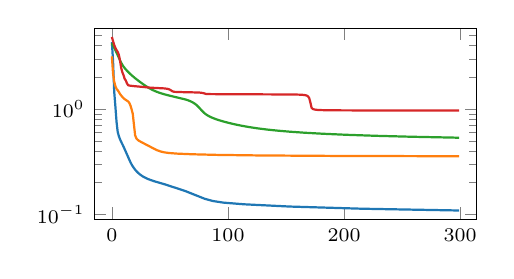
\begin{tikzpicture}

\definecolor{crimson2143940}{RGB}{214,39,40}
\definecolor{darkgray176}{RGB}{176,176,176}
\definecolor{darkorange25512714}{RGB}{255,127,14}
\definecolor{forestgreen4416044}{RGB}{44,160,44}
\definecolor{steelblue31119180}{RGB}{31,119,180}

\begin{axis}[compar,
	ymode=log]
\addplot [thick, steelblue31119180]
table {%
0 4.31118011474609
1 2.86087012290955
2 1.46213376522064
3 1.0652574300766
4 0.757783889770508
5 0.608149290084839
6 0.553772449493408
7 0.517727613449097
8 0.489268779754639
10 0.441203594207764
14 0.350765705108643
15 0.330757141113281
16 0.313158273696899
17 0.298194766044617
18 0.285662889480591
20 0.266182661056519
22 0.251716256141663
24 0.240591883659363
27 0.228317499160767
31 0.217189311981201
36 0.207478642463684
46 0.192617893218994
63 0.167274951934814
80 0.140859723091125
87 0.134231090545654
96 0.129587531089783
114 0.124923467636108
153 0.118964076042175
215 0.113466620445251
299 0.109116911888123
};
\addplot [thick, darkorange25512714]
table {%
0 3.16804385185242
1 2.1728253364563
2 1.81974112987518
3 1.65217316150665
4 1.55622470378876
5 1.50949347019196
6 1.4545316696167
7 1.39175379276276
8 1.34442985057831
9 1.30509471893311
10 1.26971399784088
11 1.24319803714752
14 1.18106353282928
15 1.14478838443756
16 1.07928073406219
17 0.99414074420929
18 0.899261236190796
19 0.711821794509888
20 0.564864158630371
21 0.529275417327881
22 0.51323676109314
23 0.502990245819092
25 0.488440990447998
36 0.422354698181152
39 0.407036423683167
42 0.396010875701904
45 0.388900637626648
49 0.383358359336853
56 0.37813663482666
69 0.372749328613281
91 0.36762523651123
127 0.363221168518066
190 0.359556078910828
299 0.356795787811279
};
\addplot [thick, forestgreen4416044]
table {%
0 4.22285127639771
1 4.01487064361572
2 3.81293964385986
3 3.61843371391296
4 3.43001246452332
5 3.24553966522217
6 3.06602549552917
7 2.89872932434082
8 2.75325393676758
9 2.63300466537476
10 2.53405690193176
11 2.45044136047363
12 2.37739825248718
13 2.31180191040039
14 2.2517294883728
15 2.19601726531982
16 2.14395308494568
17 2.09506845474243
18 2.04901480674744
19 2.00549292564392
20 1.96422600746155
22 1.88743078708649
24 1.81681656837463
26 1.75109088420868
28 1.68976640701294
30 1.63334107398987
32 1.58285140991211
34 1.53889524936676
36 1.50113666057587
38 1.46864080429077
40 1.44038474559784
42 1.41550385951996
45 1.38306832313538
48 1.35499906539917
52 1.32209038734436
63 1.23652398586273
65 1.21735787391663
67 1.1948823928833
69 1.16740524768829
70 1.15111398696899
71 1.13272404670715
72 1.11198115348816
73 1.08876585960388
75 1.03586375713348
77 0.979917526245117
78 0.953849077224731
79 0.93034839630127
80 0.909757375717163
81 0.89196240901947
82 0.876595616340637
84 0.851416349411011
86 0.831281900405884
89 0.80668306350708
92 0.786139488220215
96 0.762671232223511
101 0.737642288208008
106 0.716179132461548
112 0.694188952445984
118 0.675628066062927
125 0.657562732696533
133 0.640705108642578
142 0.625406861305237
153 0.610499143600464
166 0.596593141555786
182 0.583184480667114
202 0.570235252380371
227 0.557931184768677
258 0.54643702507019
299 0.534921646118164
};
\addplot [thick, crimson2143940]
table {%
0 4.83801460266113
1 4.40892267227173
2 4.0575966835022
3 3.81000995635986
4 3.62662363052368
5 3.4903404712677
6 3.26991677284241
7 2.88387107849121
8 2.46064591407776
9 2.23875594139099
10 2.09848737716675
11 1.93832695484161
12 1.86550188064575
13 1.75230574607849
14 1.68575251102448
15 1.67313063144684
16 1.66563010215759
18 1.65520441532135
22 1.63989841938019
27 1.62095606327057
32 1.5998467206955
35 1.59214544296265
45 1.57121884822845
47 1.56174802780151
48 1.55420339107513
49 1.54314243793488
50 1.52653920650482
52 1.47822439670563
53 1.46314704418182
54 1.45740079879761
56 1.45306062698364
61 1.44800436496735
74 1.43711578845978
76 1.43223798274994
78 1.42263174057007
79 1.4143158197403
81 1.39276945590973
82 1.3884299993515
86 1.38631105422974
103 1.38339865207672
155 1.37558126449585
161 1.37109315395355
164 1.36570847034454
166 1.35810971260071
167 1.351198554039
168 1.3394980430603
169 1.31697833538055
170 1.26625549793243
171 1.14868927001953
172 1.02802407741547
173 1.00346457958221
174 0.994166612625122
175 0.988674879074097
177 0.982434272766113
180 0.978082180023193
186 0.974670767784119
199 0.972140312194824
233 0.970206499099731
299 0.969050168991089
};
\end{axis}

\end{tikzpicture}
}
&
\multicolumn{4}{c}{% This file was created with tikzplotlib v0.10.1.
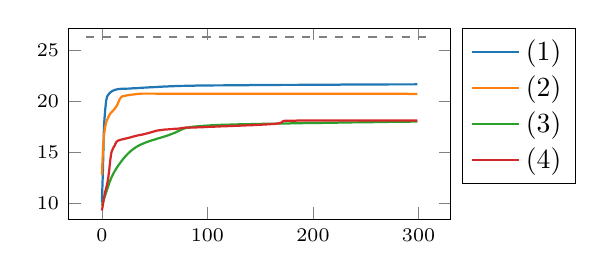
\begin{tikzpicture}

\definecolor{crimson2143940}{RGB}{214,39,40}
\definecolor{darkgray176}{RGB}{176,176,176}
\definecolor{darkorange25512714}{RGB}{255,127,14}
\definecolor{forestgreen4416044}{RGB}{44,160,44}
\definecolor{steelblue31119180}{RGB}{31,119,180}

\begin{axis}[compar, legend pos=outer north east]
\addplot [thick, steelblue31119180]
table {%
0 10.0600004196167
1 13.2399997711182
2 17.6399993896484
3 19.0200004577637
4 20.0400009155273
5 20.4799995422363
6 20.6399993896484
7 20.7700004577637
8 20.8799991607666
9 20.9599990844727
10 21.0200004577637
11 21.0699996948242
13 21.1499996185303
14 21.1700000762939
15 21.2000007629395
18 21.2299995422363
20 21.2299995422363
21 21.2399997711182
23 21.2399997711182
24 21.25
25 21.25
26 21.2600002288818
27 21.2600002288818
29 21.2800006866455
30 21.2800006866455
31 21.2900009155273
32 21.2900009155273
34 21.3099994659424
35 21.3099994659424
37 21.3299999237061
38 21.3299999237061
40 21.3500003814697
41 21.3500003814697
42 21.3600006103516
43 21.3600006103516
45 21.3799991607666
46 21.3799991607666
47 21.3899993896484
48 21.3899993896484
49 21.3999996185303
50 21.3999996185303
52 21.4200000762939
53 21.4200000762939
54 21.4300003051758
55 21.4300003051758
56 21.4400005340576
57 21.4400005340576
58 21.4500007629395
59 21.4500007629395
60 21.4599990844727
61 21.4599990844727
62 21.4699993133545
63 21.4699993133545
64 21.4799995422363
65 21.4799995422363
66 21.4899997711182
68 21.4899997711182
69 21.5
71 21.5
72 21.5100002288818
74 21.5100002288818
75 21.5200004577637
78 21.5200004577637
79 21.5300006866455
82 21.5300006866455
83 21.5400009155273
88 21.5400009155273
89 21.5499992370605
96 21.5499992370605
97 21.5599994659424
105 21.5599994659424
106 21.5699996948242
115 21.5699996948242
116 21.5799999237061
126 21.5799999237061
127 21.5900001525879
139 21.5900001525879
140 21.6000003814697
153 21.6000003814697
154 21.6100006103516
169 21.6100006103516
170 21.6200008392334
186 21.6200008392334
187 21.6299991607666
205 21.6299991607666
206 21.6399993896484
226 21.6399993896484
227 21.6499996185303
248 21.6499996185303
249 21.6599998474121
271 21.6599998474121
272 21.6700000762939
296 21.6700000762939
297 21.6800003051758
299 21.6800003051758
};
\addlegendentry{$(1)$}
\addplot [thick, darkorange25512714]
table {%
0 12.7600002288818
1 15.289999961853
2 16.6800003051758
3 17.4300003051758
4 17.9300003051758
5 18.2000007629395
6 18.4300003051758
7 18.6399993896484
8 18.8099994659424
9 18.9300003051758
10 19.0300006866455
11 19.1399993896484
12 19.2600002288818
13 19.3999996185303
14 19.5499992370605
15 19.75
16 20.0100002288818
17 20.25
18 20.3700008392334
19 20.4799995422363
20 20.5100002288818
25 20.6100006103516
26 20.6200008392334
27 20.6399993896484
28 20.6499996185303
29 20.6700000762939
31 20.6900005340576
32 20.7099990844727
36 20.75
37 20.75
38 20.7600002288818
51 20.7600002288818
52 20.75
222 20.75
223 20.7399997711182
290 20.7399997711182
291 20.7299995422363
299 20.7299995422363
};
\addlegendentry{$(2)$}
\addplot [thick, forestgreen4416044]
table {%
0 9.77999973297119
1 10.1099996566772
3 10.75
4 11.0600004196167
5 11.3800001144409
6 11.6899995803833
7 11.9899997711182
8 12.2700004577637
9 12.5200004577637
10 12.7399997711182
11 12.9399995803833
12 13.1300001144409
14 13.4700002670288
15 13.6199998855591
16 13.7799997329712
17 13.9200000762939
18 14.0699996948242
21 14.460000038147
22 14.5799999237061
24 14.8000001907349
27 15.1000003814697
28 15.1800003051758
29 15.2700004577637
30 15.3400001525879
31 15.4200000762939
32 15.4899997711182
35 15.6700000762939
38 15.8199996948242
40 15.8999996185303
41 15.9499998092651
42 15.9899997711182
43 16.0200004577637
45 16.1000003814697
46 16.1299991607666
47 16.1700000762939
51 16.2900009155273
52 16.3299999237061
58 16.5100002288818
59 16.5499992370605
61 16.6100006103516
62 16.6499996185303
63 16.6800003051758
69 16.9200000762939
72 17.0699996948242
73 17.1100006103516
76 17.2600002288818
78 17.3400001525879
80 17.3999996185303
84 17.4799995422363
85 17.4899997711182
86 17.5100002288818
95 17.6000003814697
96 17.6000003814697
98 17.6200008392334
99 17.6200008392334
101 17.6399993896484
102 17.6399993896484
103 17.6499996185303
104 17.6499996185303
105 17.6599998474121
106 17.6599998474121
107 17.6700000762939
108 17.6700000762939
109 17.6800003051758
110 17.6800003051758
111 17.6900005340576
112 17.6900005340576
113 17.7000007629395
115 17.7000007629395
116 17.7099990844727
118 17.7099990844727
119 17.7199993133545
121 17.7199993133545
122 17.7299995422363
125 17.7299995422363
126 17.7399997711182
128 17.7399997711182
129 17.75
132 17.75
133 17.7600002288818
137 17.7600002288818
138 17.7700004577637
141 17.7700004577637
142 17.7800006866455
146 17.7800006866455
147 17.7900009155273
151 17.7900009155273
152 17.7999992370605
156 17.7999992370605
157 17.8099994659424
161 17.8099994659424
162 17.8199996948242
167 17.8199996948242
168 17.8299999237061
172 17.8299999237061
173 17.8400001525879
178 17.8400001525879
179 17.8500003814697
184 17.8500003814697
185 17.8600006103516
190 17.8600006103516
191 17.8700008392334
196 17.8700008392334
197 17.8799991607666
203 17.8799991607666
204 17.8899993896484
209 17.8899993896484
210 17.8999996185303
216 17.8999996185303
217 17.9099998474121
223 17.9099998474121
224 17.9200000762939
230 17.9200000762939
231 17.9300003051758
236 17.9300003051758
237 17.9400005340576
243 17.9400005340576
244 17.9500007629395
250 17.9500007629395
251 17.9599990844727
257 17.9599990844727
258 17.9699993133545
264 17.9699993133545
265 17.9799995422363
271 17.9799995422363
272 17.9899997711182
278 17.9899997711182
279 18
285 18
286 18.0100002288818
292 18.0100002288818
293 18.0200004577637
299 18.0200004577637
};
\addlegendentry{$(3)$}
\addplot [thick, crimson2143940]
table {%
0 9.30000019073486
1 9.85999965667725
2 10.539999961853
3 11.0600004196167
4 11.4799995422363
5 11.8900003433228
6 12.4700002670288
7 13.3000001907349
8 14.289999961853
9 14.9799995422363
10 15.25
11 15.4799995422363
12 15.6400003433228
13 15.8800001144409
14 16.0599994659424
15 16.1299991607666
16 16.1800003051758
19 16.2700004577637
20 16.2900009155273
21 16.3199996948242
22 16.3400001525879
23 16.3700008392334
24 16.3899993896484
25 16.4200000762939
26 16.4400005340576
30 16.5599994659424
31 16.5799999237061
33 16.6399993896484
39 16.7600002288818
40 16.7900009155273
41 16.8099994659424
42 16.8400001525879
43 16.8600006103516
52 17.1299991607666
53 17.1399993896484
54 17.1599998474121
55 17.1700000762939
56 17.1900005340576
57 17.2000007629395
58 17.2199993133545
60 17.2399997711182
61 17.2399997711182
65 17.2800006866455
66 17.2800006866455
70 17.3199996948242
71 17.3199996948242
74 17.3500003814697
75 17.3700008392334
76 17.3799991607666
77 17.3999996185303
78 17.4099998474121
79 17.4300003051758
80 17.4400005340576
81 17.4300003051758
82 17.4300003051758
83 17.4200000762939
84 17.4300003051758
87 17.4300003051758
88 17.4400005340576
89 17.4400005340576
90 17.4500007629395
91 17.4500007629395
92 17.4599990844727
94 17.4599990844727
95 17.4699993133545
96 17.4699993133545
97 17.4799995422363
98 17.4799995422363
99 17.4899997711182
100 17.4899997711182
101 17.5
103 17.5
104 17.5100002288818
105 17.5100002288818
106 17.5200004577637
107 17.5200004577637
108 17.5300006866455
110 17.5300006866455
111 17.5400009155273
112 17.5400009155273
113 17.5499992370605
114 17.5499992370605
115 17.5599994659424
117 17.5599994659424
118 17.5699996948242
119 17.5699996948242
120 17.5799999237061
122 17.5799999237061
123 17.5900001525879
124 17.5900001525879
125 17.6000003814697
126 17.6000003814697
127 17.6100006103516
129 17.6100006103516
130 17.6200008392334
131 17.6200008392334
132 17.6299991607666
134 17.6299991607666
135 17.6399993896484
136 17.6399993896484
137 17.6499996185303
138 17.6499996185303
139 17.6599998474121
141 17.6599998474121
142 17.6700000762939
143 17.6700000762939
144 17.6800003051758
145 17.6800003051758
146 17.6900005340576
147 17.6900005340576
148 17.7000007629395
149 17.7000007629395
150 17.7099990844727
151 17.7099990844727
152 17.7199993133545
153 17.7199993133545
154 17.7299995422363
155 17.7299995422363
157 17.75
158 17.75
161 17.7800006866455
162 17.7800006866455
165 17.8099994659424
166 17.8299999237061
167 17.8400001525879
169 17.8799991607666
170 17.9200000762939
171 18.0100002288818
172 18.0799999237061
174 18.1000003814697
176 18.1000003814697
177 18.1100006103516
184 18.1100006103516
185 18.1200008392334
260 18.1200008392334
261 18.1299991607666
299 18.1299991607666
};
\addlegendentry{$(4)$}
\addplot [thick, gray, dashed]
table {%
-14.95 26.3238544464111
313.95 26.3238544464111
};
\end{axis}

\end{tikzpicture}
}
\end{tabular}
	\caption{Resultats de la LGD avec différents niveau de compression --- sans passe-bas}
	\label{fig:LGDsizes-s}
\end{figure}

\begin{figure}[H]\centering
	\begin{tabular}{c c c c c c}
	Target  &  $(1)$  &  $(2)$  &  $(3)$  &  $(4)$  &  $(5)$
	
	\\
	
	\multirow{3}{0.32\textwidth}[0.075\textwidth]{\includegraphics[width=0.32\textwidth]{resultats/LGD/sizes/size-target-g.png}}
	&
	\includegraphics[width=0.1\textwidth]{resultats/LGD/sizes/size_big-init-pas=0.2_filtre=g-0.6.png}
	&
	\includegraphics[width=0.1\textwidth]{resultats/LGD/sizes/size_mid2-init-pas=0.1_filtre=g-0.6.png}
	&
	\includegraphics[width=0.1\textwidth]{resultats/LGD/sizes/size_mid1-init-pas=0.1_filtre=g-0.6.png}
	&
	\includegraphics[width=0.1\textwidth]{resultats/LGD/sizes/size_small-init-pas=0.5_filtre=g-0.6.png}
	&
	\includegraphics[width=0.1\textwidth]{resultats/LGD/sizes/size_mini-init-pas=0.01_filtre=g-0.6.png}
	
	\\
	
	
	&
	\includegraphics[width=0.1\textwidth]{resultats/LGD/sizes/size_big-compatarget-s.png}
	&
	\includegraphics[width=0.1\textwidth]{resultats/LGD/sizes/size_mid2-compatarget-s.png}
	&
	\includegraphics[height=0.1\textwidth]{resultats/LGD/sizes/size_mid1-compatarget-s.png}
	&
	\includegraphics[width=0.1\textwidth]{resultats/LGD/sizes/size_small-compatarget-s.png}
	&
	\includegraphics[width=0.1\textwidth]{resultats/LGD/sizes/size_mini-compatarget-s.png}
	
	\\
	
	
	&
	\includegraphics[width=0.1\textwidth]{resultats/LGD/sizes/size_big-guess-pas=0.2_filtre=g-0.6.png}
	&
	\includegraphics[width=0.1\textwidth]{resultats/LGD/sizes/size_mid2-guess-pas=0.1_filtre=g-0.6.png}
	&
	\includegraphics[width=0.1\textwidth]{resultats/LGD/sizes/size_mid1-guess-pas=0.1_filtre=g-0.6.png}
	&
	\includegraphics[width=0.1\textwidth]{resultats/LGD/sizes/size_small-guess-pas=0.5_filtre=g-0.6.png}
	&
	\includegraphics[width=0.1\textwidth]{resultats/LGD/sizes/size_mini-guess-pas=0.01_filtre=g-0.6.png}
	
	\\ \\
	
	
	
	\multicolumn{2}{c}{Loss}  &  \multicolumn{4}{c}{PSNR{\color{white}bbbb}}
	
	\\
	
	\multicolumn{2}{c}{% This file was created with tikzplotlib v0.10.1.
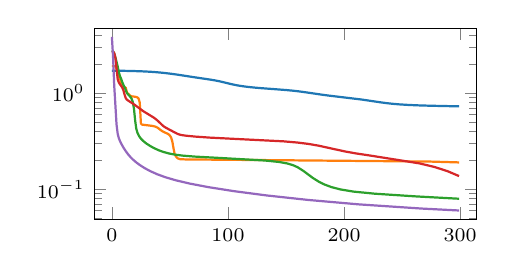
\begin{tikzpicture}

\definecolor{crimson2143940}{RGB}{214,39,40}
\definecolor{darkgray176}{RGB}{176,176,176}
\definecolor{darkorange25512714}{RGB}{255,127,14}
\definecolor{forestgreen4416044}{RGB}{44,160,44}
\definecolor{mediumpurple148103189}{RGB}{148,103,189}
\definecolor{steelblue31119180}{RGB}{31,119,180}

\begin{axis}[compar,
	ymode=log]
\addplot [thick, steelblue31119180]
table {%
0 1.72453677654266
10 1.71768462657928
18 1.709348320961
24 1.70033705234528
29 1.6901341676712
34 1.67662823200226
38 1.66295230388641
42 1.64652991294861
46 1.62746405601501
51 1.60032224655151
56 1.5699542760849
63 1.52379190921783
70 1.47829067707062
76 1.44239723682404
86 1.38365793228149
90 1.35641014575958
93 1.33313751220703
97 1.29875993728638
102 1.25543904304504
105 1.23231077194214
108 1.2123007774353
111 1.19530928134918
114 1.18089818954468
118 1.16483271121979
123 1.14839255809784
129 1.13209295272827
138 1.11113858222961
150 1.08306062221527
156 1.06606793403625
161 1.0491931438446
167 1.02564668655396
181 0.968385457992554
187 0.947251319885254
195 0.922387599945068
215 0.862796425819397
224 0.831477165222168
232 0.804347276687622
237 0.789946675300598
242 0.778159737586975
248 0.767242193222046
255 0.757997989654541
263 0.75055992603302
274 0.743492960929871
293 0.734858512878418
299 0.732345581054688
};
\addplot [thick, darkorange25512714]
table {%
0 1.93434596061707
1 1.93200349807739
2 1.92700910568237
3 1.91092967987061
4 1.82279932498932
5 1.63814675807953
6 1.49781715869904
7 1.42523396015167
8 1.27939009666443
9 1.18521678447723
10 1.17097330093384
11 1.16010677814484
12 1.13860154151917
13 1.018106341362
16 0.941693305969238
17 0.931789517402649
20 0.922242164611816
21 0.916382789611816
22 0.905909538269043
23 0.883619070053101
24 0.800576210021973
25 0.484217882156372
26 0.472478270530701
35 0.457828998565674
37 0.451737642288208
38 0.44725227355957
39 0.441246032714844
40 0.433329820632935
42 0.41453742980957
44 0.39980947971344
46 0.389489531517029
48 0.379505157470703
49 0.372840166091919
50 0.363147974014282
51 0.346918106079102
52 0.317295432090759
53 0.271204471588135
54 0.234548449516296
55 0.221139311790466
56 0.213874220848083
57 0.209440231323242
59 0.205981850624084
64 0.20487642288208
108 0.202854156494141
273 0.194810152053833
297 0.191097617149353
299 0.190571308135986
};
\addplot [thick, forestgreen4416044]
table {%
0 2.80895972251892
1 2.75048971176147
2 2.60713028907776
3 2.38255786895752
4 2.13562965393066
5 1.91229856014252
6 1.65637183189392
7 1.50856399536133
8 1.41280651092529
9 1.30485808849335
10 1.22169101238251
11 1.15476989746094
12 1.0741560459137
13 1.00716495513916
14 0.973587155342102
15 0.946269989013672
16 0.916436076164246
17 0.876654148101807
18 0.812723636627197
19 0.697008371353149
20 0.525444269180298
21 0.428455829620361
22 0.389726042747498
23 0.366618156433105
24 0.350306034088135
25 0.337761163711548
26 0.32756519317627
28 0.311413407325745
30 0.298583030700684
33 0.282851934432983
36 0.269976496696472
40 0.256317496299744
44 0.245958089828491
49 0.236628293991089
54 0.230266451835632
61 0.224518775939941
71 0.219510316848755
92 0.2126624584198
132 0.199638366699219
144 0.192842841148376
151 0.186120629310608
156 0.178535461425781
160 0.169811010360718
165 0.155425310134888
173 0.131635665893555
178 0.120536088943481
183 0.112421870231628
189 0.10558009147644
197 0.0996513366699219
208 0.0947535037994385
226 0.0901226997375488
262 0.0843832492828369
299 0.0798095464706421
};
\addplot [thick, crimson2143940]
table {%
0 2.75355887413025
1 2.72030234336853
2 2.63165354728699
3 2.34783864021301
4 1.81270730495453
5 1.40633320808411
6 1.2964209318161
7 1.23945200443268
8 1.19617938995361
9 1.146324634552
10 1.06876111030579
11 0.963654279708862
12 0.885666608810425
13 0.858596682548523
14 0.841736435890198
20 0.754436254501343
24 0.694417476654053
26 0.666041374206543
28 0.641217947006226
30 0.620044827461243
36 0.559826135635376
38 0.536990165710449
40 0.511477112770081
43 0.471526265144348
44 0.459928154945374
45 0.450082421302795
47 0.435087561607361
56 0.381032824516296
58 0.372854471206665
60 0.367727637290955
64 0.361920237541199
72 0.354321241378784
84 0.346086740493774
101 0.337772607803345
148 0.316205859184265
160 0.30713939666748
169 0.297676563262939
178 0.285158157348633
191 0.26324725151062
201 0.247857093811035
210 0.236915230751038
223 0.224390149116516
265 0.186241030693054
278 0.17077362537384
289 0.154715538024902
299 0.137419939041138
};
\addplot [thick, mediumpurple148103189]
table {%
0 3.87609815597534
1 2.41971015930176
2 1.21478092670441
3 0.759954929351807
4 0.473417043685913
5 0.378544330596924
6 0.340376138687134
7 0.318324327468872
8 0.300664186477661
9 0.285422086715698
10 0.271982550621033
12 0.249404191970825
14 0.231428861618042
16 0.216980695724487
18 0.205150842666626
21 0.190834045410156
24 0.179333209991455
28 0.166966199874878
33 0.154839515686035
39 0.143672823905945
46 0.133790850639343
55 0.124259471893311
67 0.114835143089294
83 0.105466246604919
105 0.0957608222961426
133 0.0864417552947998
169 0.0775313377380371
213 0.0696594715118408
267 0.0630255937576294
299 0.0601816177368164
};
\end{axis}

\end{tikzpicture}
}
	&
	\multicolumn{4}{c}{% This file was created with tikzplotlib v0.10.1.
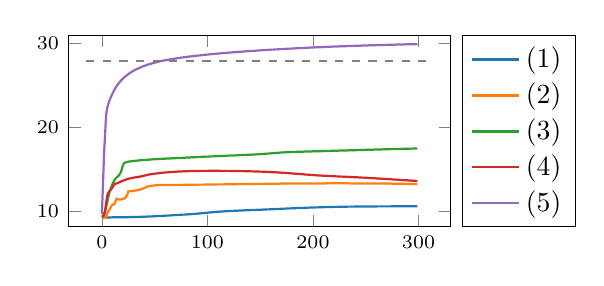
\begin{tikzpicture}

\definecolor{crimson2143940}{RGB}{214,39,40}
\definecolor{darkgray176}{RGB}{176,176,176}
\definecolor{darkorange25512714}{RGB}{255,127,14}
\definecolor{forestgreen4416044}{RGB}{44,160,44}
\definecolor{mediumpurple148103189}{RGB}{148,103,189}
\definecolor{steelblue31119180}{RGB}{31,119,180}

\begin{axis}[compar, legend pos=outer north east]
\addplot [thick, steelblue31119180]
table {%
0 9.31999969482422
9 9.31999969482422
10 9.32999992370605
17 9.32999992370605
18 9.34000015258789
22 9.34000015258789
23 9.35000038146973
26 9.35000038146973
27 9.35999965667725
30 9.35999965667725
31 9.36999988555908
33 9.36999988555908
34 9.38000011444092
36 9.38000011444092
37 9.39000034332275
38 9.39000034332275
39 9.39999961853027
40 9.39999961853027
41 9.40999984741211
42 9.40999984741211
43 9.42000007629395
44 9.42000007629395
45 9.43000030517578
46 9.43000030517578
47 9.4399995803833
48 9.4399995803833
49 9.44999980926514
50 9.44999980926514
52 9.47000026702881
53 9.47000026702881
55 9.48999977111816
56 9.48999977111816
58 9.51000022888184
59 9.51000022888184
61 9.52999973297119
62 9.52999973297119
65 9.5600004196167
66 9.5600004196167
69 9.59000015258789
70 9.59000015258789
73 9.61999988555908
74 9.61999988555908
77 9.64999961853027
78 9.64999961853027
82 9.6899995803833
83 9.6899995803833
94 9.80000019073486
95 9.81999969482422
98 9.85000038146973
99 9.86999988555908
103 9.90999984741211
104 9.93000030517578
112 10.0100002288818
113 10.0100002288818
117 10.0500001907349
118 10.0500001907349
120 10.0699996948242
121 10.0699996948242
123 10.0900001525879
124 10.0900001525879
126 10.1099996566772
127 10.1099996566772
128 10.1199998855591
129 10.1199998855591
130 10.1300001144409
131 10.1300001144409
133 10.1499996185303
134 10.1499996185303
135 10.1599998474121
136 10.1599998474121
137 10.1700000762939
138 10.1700000762939
139 10.1800003051758
140 10.1800003051758
141 10.1899995803833
142 10.1899995803833
143 10.1999998092651
144 10.1999998092651
145 10.210000038147
146 10.210000038147
147 10.2200002670288
148 10.2200002670288
149 10.2299995422363
150 10.2299995422363
151 10.2399997711182
152 10.2399997711182
153 10.25
154 10.25
155 10.2600002288818
156 10.2600002288818
157 10.2700004577637
158 10.2700004577637
159 10.2799997329712
160 10.2799997329712
161 10.289999961853
162 10.289999961853
164 10.3100004196167
165 10.3100004196167
166 10.3199996948242
167 10.3199996948242
168 10.3299999237061
169 10.3299999237061
171 10.3500003814697
172 10.3500003814697
173 10.3599996566772
174 10.3599996566772
175 10.3699998855591
176 10.3699998855591
178 10.3900003433228
179 10.3900003433228
180 10.3999996185303
181 10.3999996185303
182 10.4099998474121
183 10.4099998474121
184 10.4200000762939
185 10.4200000762939
186 10.4300003051758
187 10.4300003051758
188 10.4399995803833
189 10.4399995803833
190 10.4499998092651
191 10.4499998092651
192 10.460000038147
193 10.460000038147
194 10.4700002670288
195 10.4700002670288
196 10.4799995422363
197 10.4799995422363
198 10.4899997711182
200 10.4899997711182
201 10.5
202 10.5
203 10.5100002288818
205 10.5100002288818
206 10.5200004577637
207 10.5200004577637
208 10.5299997329712
210 10.5299997329712
211 10.539999961853
213 10.539999961853
214 10.5500001907349
216 10.5500001907349
217 10.5600004196167
219 10.5600004196167
220 10.5699996948242
223 10.5699996948242
224 10.5799999237061
227 10.5799999237061
228 10.5900001525879
232 10.5900001525879
233 10.6000003814697
239 10.6000003814697
240 10.6099996566772
248 10.6099996566772
249 10.6199998855591
260 10.6199998855591
261 10.6300001144409
274 10.6300001144409
275 10.6400003433228
287 10.6400003433228
288 10.6499996185303
299 10.6499996185303
};
\addlegendentry{$(1)$}
\addplot [thick, darkorange25512714]
table {%
0 9.28999996185303
1 9.28999996185303
2 9.30000019073486
3 9.31999969482422
4 9.4399995803833
5 9.73999977111816
6 10.0600004196167
7 10.1899995803833
8 10.4499998092651
9 10.6599998474121
10 10.8100004196167
11 10.8400001525879
12 10.9200000762939
13 11.2200002670288
14 11.5500001907349
15 11.5100002288818
16 11.460000038147
17 11.4399995803833
18 11.460000038147
19 11.4700002670288
20 11.5100002288818
21 11.5600004196167
22 11.6400003433228
23 11.75
24 12.0100002288818
25 12.3999996185303
26 12.4099998474121
27 12.4499998092651
28 12.4300003051758
29 12.4700002670288
30 12.460000038147
31 12.5
32 12.5
33 12.539999961853
34 12.5500001907349
35 12.5900001525879
36 12.6099996566772
37 12.6599998474121
38 12.6899995803833
40 12.789999961853
41 12.8599996566772
43 12.960000038147
44 13
45 13.0200004577637
46 13.0500001907349
47 13.0699996948242
48 13.0799999237061
50 13.1199998855591
51 13.1300001144409
52 13.1499996185303
53 13.1499996185303
54 13.1599998474121
60 13.1599998474121
61 13.1700000762939
69 13.1700000762939
70 13.1800003051758
77 13.1800003051758
78 13.1899995803833
84 13.1899995803833
85 13.1999998092651
91 13.1999998092651
92 13.210000038147
97 13.210000038147
98 13.2200002670288
104 13.2200002670288
105 13.2299995422363
109 13.2299995422363
110 13.2399997711182
115 13.2399997711182
116 13.25
121 13.25
122 13.2600002288818
127 13.2600002288818
128 13.2700004577637
133 13.2700004577637
134 13.2799997329712
139 13.2799997329712
140 13.289999961853
146 13.289999961853
147 13.3000001907349
153 13.3000001907349
154 13.3100004196167
160 13.3100004196167
161 13.3199996948242
168 13.3199996948242
169 13.3299999237061
178 13.3299999237061
179 13.3400001525879
190 13.3400001525879
191 13.3500003814697
211 13.3500003814697
212 13.3599996566772
234 13.3599996566772
235 13.3500003814697
255 13.3500003814697
256 13.3400001525879
266 13.3400001525879
267 13.3299999237061
274 13.3299999237061
275 13.3199996948242
280 13.3199996948242
281 13.3100004196167
285 13.3100004196167
286 13.3000001907349
289 13.3000001907349
290 13.289999961853
293 13.289999961853
294 13.2799997329712
296 13.2799997329712
297 13.2700004577637
299 13.2700004577637
};
\addlegendentry{$(2)$}
\addplot [thick, forestgreen4416044]
table {%
0 9.39999961853027
1 9.48999977111816
2 9.69999980926514
3 10.0799999237061
4 10.539999961853
5 11.039999961853
6 11.6999998092651
7 12.1999998092651
8 12.5699996948242
9 12.9499998092651
10 13.2600002288818
12 13.7399997711182
13 13.9399995803833
14 14.0600004196167
15 14.1700000762939
16 14.289999961853
17 14.460000038147
18 14.710000038147
19 15.0900001525879
20 15.5299997329712
21 15.7399997711182
22 15.8199996948242
23 15.8699998855591
25 15.9300003051758
27 15.9700002670288
28 15.9799995422363
29 16
30 16.0100002288818
31 16.0300006866455
33 16.0499992370605
34 16.0699996948242
48 16.2099990844727
49 16.2099990844727
52 16.2399997711182
53 16.2399997711182
55 16.2600002288818
56 16.2600002288818
58 16.2800006866455
59 16.2800006866455
61 16.2999992370605
62 16.2999992370605
63 16.3099994659424
64 16.3099994659424
66 16.3299999237061
67 16.3299999237061
69 16.3500003814697
70 16.3500003814697
72 16.3700008392334
73 16.3700008392334
74 16.3799991607666
75 16.3799991607666
77 16.3999996185303
78 16.3999996185303
80 16.4200000762939
81 16.4200000762939
82 16.4300003051758
83 16.4300003051758
85 16.4500007629395
86 16.4500007629395
87 16.4599990844727
88 16.4599990844727
90 16.4799995422363
91 16.4799995422363
92 16.4899997711182
93 16.4899997711182
95 16.5100002288818
96 16.5100002288818
97 16.5200004577637
98 16.5200004577637
99 16.5300006866455
100 16.5300006866455
102 16.5499992370605
103 16.5499992370605
104 16.5599994659424
105 16.5599994659424
106 16.5699996948242
107 16.5699996948242
109 16.5900001525879
110 16.5900001525879
111 16.6000003814697
112 16.6000003814697
113 16.6100006103516
114 16.6100006103516
115 16.6200008392334
116 16.6200008392334
118 16.6399993896484
119 16.6399993896484
120 16.6499996185303
121 16.6499996185303
122 16.6599998474121
123 16.6599998474121
124 16.6700000762939
125 16.6700000762939
126 16.6800003051758
127 16.6800003051758
129 16.7000007629395
130 16.7000007629395
131 16.7099990844727
132 16.7099990844727
133 16.7199993133545
134 16.7199993133545
135 16.7299995422363
136 16.7299995422363
138 16.75
139 16.75
140 16.7600002288818
141 16.7600002288818
143 16.7800006866455
144 16.7800006866455
146 16.7999992370605
147 16.7999992370605
150 16.8299999237061
151 16.8299999237061
169 17.0100002288818
170 17.0100002288818
173 17.0400009155273
174 17.0400009155273
176 17.0599994659424
177 17.0599994659424
178 17.0699996948242
179 17.0699996948242
180 17.0799999237061
181 17.0799999237061
182 17.0900001525879
183 17.0900001525879
184 17.1000003814697
186 17.1000003814697
187 17.1100006103516
188 17.1100006103516
189 17.1200008392334
191 17.1200008392334
192 17.1299991607666
194 17.1299991607666
195 17.1399993896484
197 17.1399993896484
198 17.1499996185303
199 17.1499996185303
200 17.1599998474121
202 17.1599998474121
203 17.1700000762939
205 17.1700000762939
206 17.1800003051758
208 17.1800003051758
209 17.1900005340576
211 17.1900005340576
212 17.2000007629395
214 17.2000007629395
215 17.2099990844727
216 17.2099990844727
217 17.2199993133545
219 17.2199993133545
220 17.2299995422363
222 17.2299995422363
223 17.2399997711182
224 17.2399997711182
225 17.25
227 17.25
228 17.2600002288818
230 17.2600002288818
231 17.2700004577637
233 17.2700004577637
234 17.2800006866455
235 17.2800006866455
236 17.2900009155273
238 17.2900009155273
239 17.2999992370605
241 17.2999992370605
242 17.3099994659424
243 17.3099994659424
244 17.3199996948242
246 17.3199996948242
247 17.3299999237061
249 17.3299999237061
250 17.3400001525879
252 17.3400001525879
253 17.3500003814697
255 17.3500003814697
256 17.3600006103516
257 17.3600006103516
258 17.3700008392334
260 17.3700008392334
261 17.3799991607666
263 17.3799991607666
264 17.3899993896484
266 17.3899993896484
267 17.3999996185303
269 17.3999996185303
270 17.4099998474121
272 17.4099998474121
273 17.4200000762939
275 17.4200000762939
276 17.4300003051758
278 17.4300003051758
279 17.4400005340576
281 17.4400005340576
282 17.4500007629395
284 17.4500007629395
285 17.4599990844727
287 17.4599990844727
288 17.4699993133545
291 17.4699993133545
292 17.4799995422363
294 17.4799995422363
295 17.4899997711182
297 17.4899997711182
298 17.5
299 17.5
};
\addlegendentry{$(3)$}
\addplot [thick, crimson2143940]
table {%
0 9.38000011444092
1 9.4399995803833
2 9.59000015258789
3 10.039999961853
4 11
5 11.8900003433228
6 12.210000038147
7 12.3999996185303
8 12.539999961853
9 12.6899995803833
10 12.8800001144409
11 13.1000003814697
12 13.25
13 13.3100004196167
17 13.5100002288818
18 13.5699996948242
19 13.6199998855591
20 13.6800003051758
22 13.7799997329712
25 13.8999996185303
28 13.9899997711182
29 14.0100002288818
30 14.039999961853
37 14.1800003051758
44 14.3900003433228
50 14.5100002288818
51 14.5200004577637
53 14.5600004196167
54 14.5699996948242
55 14.5900001525879
56 14.6000003814697
57 14.6199998855591
69 14.7399997711182
70 14.7399997711182
72 14.7600002288818
73 14.7600002288818
75 14.7799997329712
76 14.7799997329712
77 14.789999961853
78 14.789999961853
79 14.8000001907349
81 14.8000001907349
82 14.8100004196167
84 14.8100004196167
85 14.8199996948242
87 14.8199996948242
88 14.8299999237061
92 14.8299999237061
93 14.8400001525879
100 14.8400001525879
101 14.8500003814697
111 14.8500003814697
112 14.8400001525879
121 14.8400001525879
122 14.8299999237061
126 14.8299999237061
127 14.8199996948242
131 14.8199996948242
132 14.8100004196167
135 14.8100004196167
136 14.8000001907349
138 14.8000001907349
139 14.789999961853
141 14.789999961853
142 14.7799997329712
144 14.7799997329712
145 14.7700004577637
146 14.7700004577637
147 14.7600002288818
149 14.7600002288818
150 14.75
151 14.75
152 14.7399997711182
153 14.7399997711182
154 14.7299995422363
155 14.7299995422363
156 14.7200002670288
157 14.7200002670288
158 14.710000038147
159 14.710000038147
161 14.6899995803833
162 14.6899995803833
164 14.6700000762939
165 14.6700000762939
167 14.6499996185303
168 14.6499996185303
172 14.6099996566772
173 14.6099996566772
200 14.3400001525879
201 14.3400001525879
205 14.3000001907349
206 14.3000001907349
209 14.2700004577637
210 14.2700004577637
212 14.25
213 14.25
215 14.2299995422363
216 14.2299995422363
217 14.2200002670288
218 14.2200002670288
220 14.1999998092651
221 14.1999998092651
222 14.1899995803833
223 14.1899995803833
224 14.1800003051758
225 14.1800003051758
227 14.1599998474121
228 14.1599998474121
229 14.1499996185303
230 14.1499996185303
231 14.1400003433228
232 14.1400003433228
234 14.1199998855591
235 14.1199998855591
236 14.1099996566772
237 14.1099996566772
239 14.0900001525879
240 14.0900001525879
241 14.0799999237061
242 14.0799999237061
244 14.0600004196167
245 14.0600004196167
247 14.039999961853
248 14.039999961853
250 14.0200004577637
251 14.0200004577637
254 13.9899997711182
255 13.9899997711182
257 13.9700002670288
258 13.9700002670288
262 13.9300003051758
263 13.9300003051758
266 13.8999996185303
267 13.8999996185303
271 13.8599996566772
272 13.8599996566772
276 13.8199996948242
277 13.8199996948242
282 13.7700004577637
283 13.7700004577637
286 13.7399997711182
287 13.7399997711182
291 13.6999998092651
292 13.6999998092651
295 13.6700000762939
296 13.6700000762939
298 13.6499996185303
299 13.6499996185303
};
\addlegendentry{$(4)$}
\addplot [thick, mediumpurple148103189]
table {%
0 9.72999954223633
1 13.0900001525879
2 16.6800003051758
3 19.1000003814697
4 21.4699993133545
5 22.2900009155273
6 22.7399997711182
7 23.1100006103516
8 23.4300003051758
9 23.7299995422363
10 24.0100002288818
11 24.2600002288818
12 24.4899997711182
13 24.7099990844727
14 24.8999996185303
15 25.0799999237061
16 25.25
17 25.3999996185303
19 25.6800003051758
21 25.9200000762939
22 26.0300006866455
24 26.2299995422363
26 26.4099998474121
29 26.6499996185303
31 26.7900009155273
32 26.8500003814697
33 26.9200000762939
35 27.0400009155273
37 27.1399993896484
38 27.2000007629395
39 27.25
40 27.2900009155273
41 27.3400001525879
43 27.4200000762939
44 27.4699993133545
45 27.5
47 27.5799999237061
48 27.6100006103516
49 27.6499996185303
51 27.7099990844727
52 27.75
54 27.8099994659424
55 27.8299999237061
57 27.8899993896484
58 27.9099998474121
60 27.9699993133545
62 28.0100002288818
63 28.0400009155273
75 28.2800006866455
76 28.2900009155273
79 28.3500003814697
80 28.3600006103516
81 28.3799991607666
82 28.3899993896484
83 28.4099998474121
84 28.4200000762939
85 28.4400005340576
86 28.4500007629395
87 28.4699993133545
88 28.4799995422363
89 28.5
90 28.5100002288818
91 28.5300006866455
93 28.5499992370605
94 28.5699996948242
96 28.5900001525879
97 28.6100006103516
100 28.6399993896484
101 28.6599998474121
105 28.7000007629395
106 28.7199993133545
112 28.7800006866455
113 28.7999992370605
132 28.9899997711182
133 28.9899997711182
141 29.0699996948242
142 29.0699996948242
148 29.1299991607666
149 29.1299991607666
153 29.1700000762939
154 29.1700000762939
157 29.2000007629395
158 29.2000007629395
161 29.2299995422363
162 29.2299995422363
165 29.2600002288818
166 29.2600002288818
169 29.2900009155273
170 29.2900009155273
172 29.3099994659424
173 29.3099994659424
175 29.3299999237061
176 29.3299999237061
178 29.3500003814697
179 29.3500003814697
181 29.3700008392334
182 29.3700008392334
184 29.3899993896484
185 29.3899993896484
187 29.4099998474121
188 29.4099998474121
190 29.4300003051758
191 29.4300003051758
192 29.4400005340576
193 29.4400005340576
195 29.4599990844727
196 29.4599990844727
197 29.4699993133545
198 29.4699993133545
199 29.4799995422363
200 29.4799995422363
202 29.5
203 29.5
204 29.5100002288818
205 29.5100002288818
206 29.5200004577637
207 29.5200004577637
208 29.5300006866455
209 29.5300006866455
210 29.5400009155273
211 29.5400009155273
213 29.5599994659424
214 29.5599994659424
215 29.5699996948242
216 29.5699996948242
217 29.5799999237061
218 29.5799999237061
219 29.5900001525879
220 29.5900001525879
221 29.6000003814697
222 29.6000003814697
223 29.6100006103516
224 29.6100006103516
225 29.6200008392334
227 29.6200008392334
228 29.6299991607666
229 29.6299991607666
230 29.6399993896484
231 29.6399993896484
232 29.6499996185303
233 29.6499996185303
234 29.6599998474121
235 29.6599998474121
236 29.6700000762939
238 29.6700000762939
239 29.6800003051758
240 29.6800003051758
241 29.6900005340576
242 29.6900005340576
243 29.7000007629395
245 29.7000007629395
246 29.7099990844727
247 29.7099990844727
248 29.7199993133545
250 29.7199993133545
251 29.7299995422363
252 29.7299995422363
253 29.7399997711182
255 29.7399997711182
256 29.75
258 29.75
259 29.7600002288818
260 29.7600002288818
261 29.7700004577637
263 29.7700004577637
264 29.7800006866455
266 29.7800006866455
267 29.7900009155273
269 29.7900009155273
270 29.7999992370605
272 29.7999992370605
273 29.8099994659424
275 29.8099994659424
276 29.8199996948242
278 29.8199996948242
279 29.8299999237061
281 29.8299999237061
282 29.8400001525879
284 29.8400001525879
285 29.8500003814697
287 29.8500003814697
288 29.8600006103516
291 29.8600006103516
292 29.8700008392334
294 29.8700008392334
295 29.8799991607666
298 29.8799991607666
299 29.8899993896484
};
\addlegendentry{$(5)$}
\addplot [thick, gray, dashed]
table {%
-14.95 27.8502388000488
313.95 27.8502388000488
};
\end{axis}

\end{tikzpicture}
}
\end{tabular}
	\caption{Idem, cette fois avec un passe-bas gaussien ($\sigma=0.5$)}
	\label{fig:LGDsizes-g}
\end{figure}
%\\ \\



\subsection{Variation de la taille de l'espace latent}\label{sec:LGDlat}

Toujours dans l'optique de voir les limites de la méthodes, trois autres auto-encodeurs ont été entraînés avec différentes taille d'espace latent. Pour chaque --- \textit{fig. \ref{fig:LGDlat100-s}} à \textit{ \ref{fig:LGDlat800-g}} --- la LGD est effectuée avec différentes initialisations (toujours en première ligne). En fonction des cas, la loss fait parfois des zig-zags, ce qui indique que le pas est parfois trop grand. Mais même sachant cela, les résultats sont étonnamment bons. En particulier pour le deux dernières figures, où $d=800$ ce qui est plus que la taille des images, à savoir $28\times28=784$. \`A noter tout de même qu'à mesure que $d$ augmente les PSNR reste de plus en plus loin du PSNR de référence (PSNR$(\bf{x_0}, f(\bf{x_0}))$), qui lui reste globalement stable.
\\

\newpage

\begin{figure}[H]\centering
    \begin{tabular}{c c c c c c}
Target  &  $(1)$  &  $(2)$  &  $(3)$  &  $(4)$  &  $(5)$

\\

\multirow{3}{0.3\textwidth}[0.05\textwidth]{\includegraphics[width=0.3\textwidth]{resultats/LGD/sizes/size-target-s.png}}
&
\includegraphics[width=0.12\textwidth]{resultats/LGD/sizes/size_big-init-pas=0.1_filtre=s-None.png}
&
\includegraphics[width=0.12\textwidth]{resultats/LGD/sizes/size_mid2-init-pas=0.1_filtre=s-None.png}
&
\includegraphics[width=0.12\textwidth]{resultats/LGD/sizes/size_mid1-init-pas=0.1_filtre=s-None.png}
&
\includegraphics[width=0.12\textwidth]{resultats/LGD/sizes/size_small-init-pas=0.05_filtre=s-None.png}
&
\includegraphics[width=0.12\textwidth]{resultats/LGD/sizes/size_mini-init-pas=0.01_filtre=s-None.png}

\\


&
\includegraphics[width=0.12\textwidth]{resultats/LGD/sizes/size_big-compatarget-s.png}
&
\includegraphics[width=0.12\textwidth]{resultats/LGD/sizes/size_mid2-compatarget-s.png}
&
\includegraphics[height=0.12\textwidth]{resultats/LGD/sizes/size_mid1-compatarget-s.png}
&
\includegraphics[width=0.12\textwidth]{resultats/LGD/sizes/size_small-compatarget-s.png}
&
\includegraphics[width=0.12\textwidth]{resultats/LGD/sizes/size_mini-compatarget-s.png}

\\


&
\includegraphics[width=0.12\textwidth]{resultats/LGD/sizes/size_big-guess-pas=0.1_filtre=s-None.png}
&
\includegraphics[width=0.12\textwidth]{resultats/LGD/sizes/size_mid2-guess-pas=0.1_filtre=s-None.png}
&
\includegraphics[width=0.12\textwidth]{resultats/LGD/sizes/size_mid1-guess-pas=0.1_filtre=s-None.png}
&
\includegraphics[width=0.12\textwidth]{resultats/LGD/sizes/size_small-guess-pas=0.05_filtre=s-None.png}
&
\includegraphics[width=0.12\textwidth]{resultats/LGD/sizes/size_mini-guess-pas=0.01_filtre=s-None.png}

\\ \\



\multicolumn{2}{c}{Loss}  &  \multicolumn{4}{c}{PSNR{\color{white}bbbb}}

\\

\multicolumn{2}{c}{% This file was created with tikzplotlib v0.10.1.
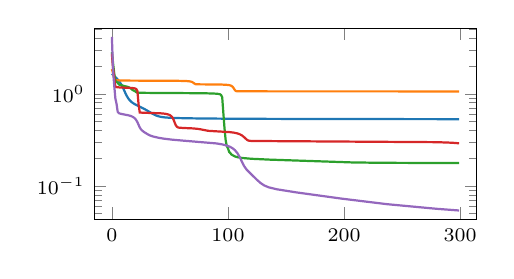
\begin{tikzpicture}

\definecolor{crimson2143940}{RGB}{214,39,40}
\definecolor{darkgray176}{RGB}{176,176,176}
\definecolor{darkorange25512714}{RGB}{255,127,14}
\definecolor{forestgreen4416044}{RGB}{44,160,44}
\definecolor{mediumpurple148103189}{RGB}{148,103,189}
\definecolor{steelblue31119180}{RGB}{31,119,180}

\begin{axis}[compar,
	ymode=log]
\addplot [thick, steelblue31119180]
table {%
0 1.65230560302734
1 1.60967218875885
3 1.51980757713318
5 1.4276807308197
6 1.37903583049774
7 1.32599353790283
8 1.26667380332947
9 1.20057117938995
11 1.05875587463379
12 0.993848085403442
13 0.939155459403992
14 0.895524501800537
15 0.861427426338196
16 0.834641695022583
17 0.813176393508911
18 0.795508742332458
19 0.780535697937012
21 0.755721092224121
24 0.724630355834961
28 0.684367299079895
32 0.640052795410156
35 0.6075519323349
37 0.589563608169556
39 0.575842380523682
41 0.56618332862854
43 0.559664726257324
46 0.553641200065613
50 0.549216270446777
57 0.545149207115173
70 0.541172504425049
93 0.53755521774292
135 0.534475564956665
221 0.531806707382202
299 0.530493259429932
};
\addplot [thick, darkorange25512714]
table {%
0 1.85211646556854
1 1.67770111560822
2 1.46272897720337
3 1.41593718528748
4 1.40484702587128
5 1.39981067180634
7 1.39501214027405
10 1.39188122749329
16 1.38930439949036
32 1.38671922683716
55 1.38247323036194
61 1.37871134281158
64 1.3742892742157
66 1.36830806732178
67 1.36319196224213
68 1.3552680015564
69 1.34236979484558
70 1.32132458686829
71 1.292635679245
72 1.27158439159393
73 1.26629757881165
76 1.26518905162811
89 1.26179456710815
95 1.25753927230835
98 1.25268864631653
100 1.24624443054199
101 1.24075663089752
102 1.23218429088593
103 1.21773552894592
104 1.191610455513
105 1.1454873085022
106 1.09121680259705
107 1.06940352916718
108 1.06570613384247
111 1.06433713436127
144 1.06147050857544
275 1.06137251853943
299 1.06136870384216
};
\addplot [thick, forestgreen4416044]
table {%
0 2.84194612503052
1 2.15506029129028
2 1.66873693466187
3 1.38294208049774
5 1.31623303890228
6 1.26444888114929
7 1.24834167957306
9 1.23046517372131
11 1.20998632907867
13 1.19424068927765
14 1.18405818939209
15 1.1702915430069
16 1.15001618862152
17 1.1210218667984
18 1.09569573402405
19 1.08197319507599
20 1.06478106975555
21 1.0405730009079
22 1.02683997154236
25 1.02437090873718
35 1.02164471149445
77 1.01418256759644
85 1.00862324237823
89 1.00375008583069
91 0.999232292175293
92 0.9952312707901
93 0.988119006156921
94 0.972235679626465
95 0.91933798789978
96 0.616937160491943
97 0.421802282333374
98 0.312908411026001
99 0.270792961120605
100 0.255544066429138
101 0.234020471572876
102 0.227557420730591
103 0.219099283218384
106 0.209146738052368
108 0.20545756816864
112 0.201385498046875
120 0.197391390800476
136 0.193149089813232
207 0.180134654045105
232 0.178421974182129
299 0.177336454391479
};
\addplot [thick, crimson2143940]
table {%
0 2.71224212646484
1 1.89663374423981
2 1.51032817363739
3 1.19073891639709
4 1.18067479133606
6 1.17347884178162
9 1.16805064678192
17 1.15556478500366
19 1.1488208770752
20 1.14171743392944
21 1.12556207180023
22 1.0690438747406
23 0.763562440872192
24 0.626803040504456
26 0.623935461044312
42 0.614003896713257
45 0.609050154685974
47 0.603470325469971
49 0.593772172927856
50 0.585844755172729
51 0.574084281921387
52 0.555935382843018
53 0.527923822402954
54 0.490156412124634
55 0.456605553627014
56 0.438905239105225
57 0.431463479995728
58 0.428577065467834
61 0.426207780838013
70 0.421022057533264
74 0.416285991668701
77 0.410333037376404
83 0.396579504013062
88 0.392909526824951
101 0.38445782661438
105 0.37907612323761
108 0.372137427330017
110 0.364766120910645
112 0.353622436523438
114 0.337481260299683
116 0.319562911987305
117 0.313272714614868
118 0.309869647026062
120 0.30800199508667
132 0.30707573890686
280 0.298706293106079
293 0.294538974761963
299 0.290218830108643
};
\addplot [thick, mediumpurple148103189]
table {%
0 4.13749027252197
1 1.78226494789124
2 1.23609900474548
3 0.890265941619873
4 0.779228687286377
5 0.638609528541565
6 0.617340087890625
7 0.609525799751282
9 0.601629018783569
14 0.585130453109741
16 0.575769901275635
17 0.569563150405884
18 0.561703205108643
19 0.551372528076172
20 0.537355184555054
21 0.517969131469727
22 0.491822361946106
23 0.46056592464447
24 0.431907415390015
25 0.412346363067627
26 0.399762630462646
28 0.382634878158569
31 0.362732648849487
33 0.35280454158783
36 0.34282374382019
40 0.333760499954224
45 0.325755834579468
52 0.317875027656555
63 0.309140682220459
90 0.289501667022705
95 0.28264594078064
99 0.274349570274353
102 0.264988541603088
104 0.256195902824402
106 0.244262218475342
108 0.227995634078979
110 0.206859588623047
113 0.172638773918152
114 0.163624286651611
116 0.150722026824951
119 0.13795006275177
125 0.116512775421143
128 0.107834815979004
131 0.10168719291687
135 0.0967668294906616
142 0.0921484231948853
159 0.0851820707321167
198 0.0729167461395264
237 0.0635035037994385
279 0.0566712617874146
299 0.0542340278625488
};
\end{axis}

\end{tikzpicture}
}
&
\multicolumn{4}{c}{% This file was created with tikzplotlib v0.10.1.
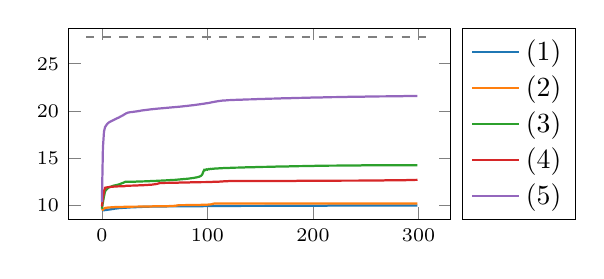
\begin{tikzpicture}

\definecolor{crimson2143940}{RGB}{214,39,40}
\definecolor{darkgray176}{RGB}{176,176,176}
\definecolor{darkorange25512714}{RGB}{255,127,14}
\definecolor{forestgreen4416044}{RGB}{44,160,44}
\definecolor{mediumpurple148103189}{RGB}{148,103,189}
\definecolor{steelblue31119180}{RGB}{31,119,180}

\begin{axis}[compar, legend pos=outer north east]
\addplot [thick, steelblue31119180]
table {%
0 9.43000030517578
1 9.44999980926514
3 9.47000026702881
4 9.48999977111816
5 9.5
6 9.52000045776367
7 9.52999973297119
9 9.56999969482422
10 9.57999992370605
13 9.64000034332275
15 9.65999984741211
16 9.68000030517578
18 9.69999980926514
19 9.69999980926514
22 9.72999954223633
23 9.72999954223633
25 9.75
26 9.75
27 9.76000022888184
28 9.76000022888184
29 9.77000045776367
30 9.77000045776367
31 9.77999973297119
32 9.77999973297119
34 9.80000019073486
35 9.80000019073486
36 9.8100004196167
38 9.8100004196167
39 9.81999969482422
40 9.81999969482422
41 9.82999992370605
44 9.82999992370605
45 9.84000015258789
48 9.84000015258789
49 9.85000038146973
54 9.85000038146973
55 9.85999965667725
61 9.85999965667725
62 9.86999988555908
71 9.86999988555908
72 9.88000011444092
82 9.88000011444092
83 9.89000034332275
96 9.89000034332275
97 9.89999961853027
112 9.89999961853027
113 9.90999984741211
131 9.90999984741211
132 9.92000007629395
154 9.92000007629395
155 9.93000030517578
181 9.93000030517578
182 9.9399995803833
213 9.9399995803833
214 9.94999980926514
251 9.94999980926514
252 9.96000003814697
295 9.96000003814697
296 9.97000026702881
299 9.97000026702881
};
\addlegendentry{$(1)$}
\addplot [thick, darkorange25512714]
table {%
0 9.4399995803833
1 9.52000045776367
2 9.64000034332275
3 9.6899995803833
4 9.72000026702881
5 9.72999954223633
6 9.75
7 9.76000022888184
8 9.76000022888184
10 9.77999973297119
11 9.77999973297119
12 9.78999996185303
14 9.78999996185303
15 9.80000019073486
16 9.80000019073486
17 9.8100004196167
20 9.8100004196167
21 9.81999969482422
24 9.81999969482422
25 9.82999992370605
29 9.82999992370605
30 9.84000015258789
34 9.84000015258789
35 9.85000038146973
40 9.85000038146973
41 9.85999965667725
47 9.85999965667725
48 9.86999988555908
53 9.86999988555908
54 9.88000011444092
59 9.88000011444092
60 9.89000034332275
63 9.89000034332275
64 9.89999961853027
66 9.89999961853027
70 9.9399995803833
72 9.97999954223633
74 10
79 10
80 10.0100002288818
87 10.0100002288818
88 10.0200004577637
93 10.0200004577637
94 10.0299997329712
97 10.0299997329712
98 10.039999961853
99 10.039999961853
103 10.0799999237061
104 10.1000003814697
106 10.1599998474121
107 10.1700000762939
170 10.1700000762939
171 10.1800003051758
299 10.1800003051758
};
\addlegendentry{$(2)$}
\addplot [thick, forestgreen4416044]
table {%
0 9.60999965667725
1 10.289999961853
2 10.9300003051758
3 11.4499998092651
4 11.6199998855591
5 11.710000038147
6 11.8199996948242
7 11.9099998474121
8 11.9399995803833
11 12.0600004196167
12 12.0900001525879
13 12.1099996566772
14 12.1400003433228
15 12.1599998474121
16 12.1899995803833
17 12.2299995422363
18 12.2799997329712
20 12.3599996566772
21 12.4099998474121
22 12.4700002670288
23 12.4799995422363
27 12.4799995422363
28 12.4899997711182
32 12.4899997711182
33 12.5
35 12.5
36 12.5100002288818
38 12.5100002288818
39 12.5200004577637
40 12.5200004577637
41 12.5299997329712
43 12.5299997329712
44 12.539999961853
45 12.539999961853
46 12.5500001907349
47 12.5500001907349
48 12.5600004196167
49 12.5600004196167
50 12.5699996948242
51 12.5699996948242
52 12.5799999237061
53 12.5799999237061
55 12.6000003814697
56 12.6000003814697
57 12.6099996566772
58 12.6099996566772
59 12.6199998855591
60 12.6199998855591
62 12.6400003433228
63 12.6400003433228
65 12.6599998474121
66 12.6599998474121
68 12.6800003051758
69 12.6800003051758
82 12.8100004196167
83 12.8299999237061
84 12.8400001525879
85 12.8599996566772
86 12.8699998855591
90 12.9499998092651
92 13.0100002288818
93 13.0500001907349
94 13.1199998855591
95 13.2299995422363
96 13.5100002288818
97 13.75
98 13.7200002670288
99 13.8000001907349
100 13.7600002288818
101 13.8299999237061
102 13.8100004196167
103 13.8500003814697
104 13.8400001525879
105 13.8699998855591
106 13.8599996566772
107 13.8800001144409
108 13.8800001144409
109 13.8900003433228
110 13.8900003433228
111 13.9099998474121
112 13.9099998474121
113 13.9200000762939
114 13.9200000762939
115 13.9300003051758
117 13.9300003051758
118 13.9399995803833
119 13.9399995803833
120 13.9499998092651
121 13.9499998092651
122 13.960000038147
124 13.960000038147
125 13.9700002670288
126 13.9700002670288
127 13.9799995422363
129 13.9799995422363
130 13.9899997711182
132 13.9899997711182
133 14
135 14
136 14.0100002288818
138 14.0100002288818
139 14.0200004577637
142 14.0200004577637
143 14.0299997329712
145 14.0299997329712
146 14.039999961853
149 14.039999961853
150 14.0500001907349
152 14.0500001907349
153 14.0600004196167
156 14.0600004196167
157 14.0699996948242
160 14.0699996948242
161 14.0799999237061
164 14.0799999237061
165 14.0900001525879
168 14.0900001525879
169 14.1000003814697
172 14.1000003814697
173 14.1099996566772
177 14.1099996566772
178 14.1199998855591
181 14.1199998855591
182 14.1300001144409
186 14.1300001144409
187 14.1400003433228
190 14.1400003433228
191 14.1499996185303
195 14.1499996185303
196 14.1599998474121
201 14.1599998474121
202 14.1700000762939
207 14.1700000762939
208 14.1800003051758
214 14.1800003051758
215 14.1899995803833
222 14.1899995803833
223 14.1999998092651
232 14.1999998092651
233 14.210000038147
245 14.210000038147
246 14.2200002670288
262 14.2200002670288
263 14.2299995422363
281 14.2299995422363
282 14.2399997711182
299 14.2399997711182
};
\addlegendentry{$(3)$}
\addplot [thick, crimson2143940]
table {%
0 9.85000038146973
1 10.7600002288818
2 11.4700002670288
3 11.8400001525879
4 11.8699998855591
5 11.8900003433228
6 11.8999996185303
7 11.9200000762939
12 11.9700002670288
13 11.9700002670288
15 11.9899997711182
16 11.9899997711182
17 12
18 12
19 12.0100002288818
21 12.0100002288818
22 12.0200004577637
23 12.0600004196167
27 12.0600004196167
28 12.0699996948242
29 12.0699996948242
30 12.0799999237061
32 12.0799999237061
33 12.0900001525879
34 12.0900001525879
35 12.1000003814697
36 12.1000003814697
37 12.1099996566772
38 12.1099996566772
39 12.1199998855591
40 12.1199998855591
42 12.1400003433228
43 12.1400003433228
45 12.1599998474121
46 12.1599998474121
48 12.1800003051758
49 12.1999998092651
50 12.210000038147
52 12.25
55 12.3400001525879
56 12.3500003814697
59 12.3500003814697
60 12.3599996566772
63 12.3599996566772
64 12.3699998855591
68 12.3699998855591
69 12.3800001144409
72 12.3800001144409
73 12.3900003433228
76 12.3900003433228
77 12.3999996185303
80 12.3999996185303
81 12.4099998474121
83 12.4099998474121
84 12.4200000762939
88 12.4200000762939
89 12.4300003051758
93 12.4300003051758
94 12.4399995803833
98 12.4399995803833
99 12.4499998092651
101 12.4499998092651
102 12.460000038147
104 12.460000038147
105 12.4700002670288
107 12.4700002670288
108 12.4799995422363
109 12.4799995422363
110 12.4899997711182
111 12.4899997711182
112 12.5
113 12.5
116 12.5299997329712
117 12.5299997329712
118 12.539999961853
119 12.539999961853
120 12.5500001907349
136 12.5500001907349
137 12.5600004196167
160 12.5600004196167
161 12.5699996948242
184 12.5699996948242
185 12.5799999237061
207 12.5799999237061
208 12.5900001525879
226 12.5900001525879
227 12.6000003814697
243 12.6000003814697
244 12.6099996566772
257 12.6099996566772
258 12.6199998855591
267 12.6199998855591
268 12.6300001144409
276 12.6300001144409
277 12.6400003433228
283 12.6400003433228
284 12.6499996185303
288 12.6499996185303
289 12.6599998474121
292 12.6599998474121
293 12.6700000762939
296 12.6700000762939
297 12.6800003051758
298 12.6800003051758
299 12.6899995803833
};
\addlegendentry{$(4)$}
\addplot [thick, mediumpurple148103189]
table {%
0 10.3500003814697
1 16.1200008392334
2 17.7999992370605
3 18.2800006866455
4 18.4400005340576
5 18.6100006103516
6 18.7099990844727
7 18.7999992370605
9 18.9200000762939
10 18.9699993133545
11 19.0300006866455
12 19.0799999237061
13 19.1399993896484
14 19.1900005340576
15 19.25
16 19.2900009155273
17 19.3600006103516
18 19.4099998474121
19 19.4799995422363
20 19.5300006866455
21 19.6100006103516
22 19.6700000762939
23 19.7399997711182
24 19.7800006866455
25 19.8299999237061
26 19.8400001525879
27 19.8700008392334
28 19.8700008392334
29 19.8899993896484
30 19.8999996185303
31 19.9200000762939
32 19.9300003051758
33 19.9500007629395
34 19.9599990844727
35 19.9899997711182
36 20
37 20.0300006866455
38 20.0400009155273
39 20.0599994659424
40 20.0699996948242
41 20.0900001525879
42 20.1000003814697
43 20.1200008392334
44 20.1299991607666
45 20.1499996185303
48 20.1800003051758
49 20.2000007629395
50 20.2000007629395
51 20.2199993133545
76 20.4699993133545
77 20.4899997711182
81 20.5300006866455
82 20.5499992370605
84 20.5699996948242
85 20.5900001525879
87 20.6100006103516
88 20.6299991607666
89 20.6399993896484
90 20.6599998474121
91 20.6700000762939
92 20.6900005340576
93 20.7000007629395
95 20.7399997711182
96 20.75
99 20.8099994659424
100 20.8199996948242
103 20.8799991607666
104 20.9099998474121
111 21.0499992370605
113 21.0699996948242
114 21.0900001525879
116 21.1100006103516
117 21.1100006103516
120 21.1399993896484
121 21.1399993896484
122 21.1499996185303
123 21.1499996185303
124 21.1599998474121
125 21.1599998474121
126 21.1700000762939
127 21.1700000762939
128 21.1800003051758
130 21.1800003051758
131 21.1900005340576
133 21.1900005340576
134 21.2000007629395
135 21.2000007629395
136 21.2099990844727
138 21.2099990844727
139 21.2199993133545
141 21.2199993133545
142 21.2299995422363
143 21.2299995422363
144 21.2399997711182
146 21.2399997711182
147 21.25
149 21.25
150 21.2600002288818
152 21.2600002288818
153 21.2700004577637
154 21.2700004577637
155 21.2800006866455
157 21.2800006866455
158 21.2900009155273
160 21.2900009155273
161 21.2999992370605
163 21.2999992370605
164 21.3099994659424
166 21.3099994659424
167 21.3199996948242
169 21.3199996948242
170 21.3299999237061
172 21.3299999237061
173 21.3400001525879
176 21.3400001525879
177 21.3500003814697
179 21.3500003814697
180 21.3600006103516
182 21.3600006103516
183 21.3700008392334
186 21.3700008392334
187 21.3799991607666
189 21.3799991607666
190 21.3899993896484
193 21.3899993896484
194 21.3999996185303
197 21.3999996185303
198 21.4099998474121
201 21.4099998474121
202 21.4200000762939
205 21.4200000762939
206 21.4300003051758
209 21.4300003051758
210 21.4400005340576
213 21.4400005340576
214 21.4500007629395
217 21.4500007629395
218 21.4599990844727
222 21.4599990844727
223 21.4699993133545
227 21.4699993133545
228 21.4799995422363
232 21.4799995422363
233 21.4899997711182
238 21.4899997711182
239 21.5
243 21.5
244 21.5100002288818
249 21.5100002288818
250 21.5200004577637
255 21.5200004577637
256 21.5300006866455
262 21.5300006866455
263 21.5400009155273
269 21.5400009155273
270 21.5499992370605
277 21.5499992370605
278 21.5599994659424
285 21.5599994659424
286 21.5699996948242
294 21.5699996948242
295 21.5799999237061
299 21.5799999237061
};
\addlegendentry{$(5)$}
\addplot [thick, gray, dashed]
table {%
-14.95 27.8502388000488
313.95 27.8502388000488
};
\end{axis}

\end{tikzpicture}
}
\end{tabular}
    \caption{$d=100$, sans passe-base}
    \label{fig:LGDlat100-s}
\end{figure}

\begin{figure}[H]\centering
	\begin{tabular}{c c c c c c}
	Target  &  $(1)$  &  $(2)$  &  $(3)$   &  $(4)$ &  $(5)$
	
	\\
	
	\multirow{2}{0.25\textwidth}[0.1\textwidth]{\includegraphics[width=0.25\textwidth]{resultats/LGD/lats/lat-100-target-g.png}}
	&
	\includegraphics[width=0.12\textwidth]{resultats/LGD/lats/lat-100_1-init-pas=0.25_filtre=g-0.6.png}
	&
	\includegraphics[width=0.12\textwidth]{resultats/LGD/lats/lat-100_2-init-pas=0.25_filtre=g-0.6.png}
	&
	\includegraphics[width=0.12\textwidth]{resultats/LGD/lats/lat-100_3-init-pas=0.25_filtre=g-0.6.png}
	&
	\includegraphics[width=0.12\textwidth]{resultats/LGD/lats/lat-100_4-init-pas=0.25_filtre=g-0.6.png}
	&
	\includegraphics[width=0.12\textwidth]{resultats/LGD/lats/lat-100_5-init-pas=0.25_filtre=g-0.6.png}
	
	\\
	
	
	&
	\includegraphics[width=0.12\textwidth]{resultats/LGD/lats/lat-100_1-guess-pas=0.25_filtre=g-0.6.png}
	&
	\includegraphics[width=0.12\textwidth]{resultats/LGD/lats/lat-100_2-guess-pas=0.25_filtre=g-0.6.png}
	&
	\includegraphics[width=0.12\textwidth]{resultats/LGD/lats/lat-100_3-guess-pas=0.25_filtre=g-0.6.png}
	&
	\includegraphics[width=0.12\textwidth]{resultats/LGD/lats/lat-100_4-guess-pas=0.25_filtre=g-0.6.png}
	&
	\includegraphics[width=0.12\textwidth]{resultats/LGD/lats/lat-100_5-guess-pas=0.25_filtre=g-0.6.png}
	
	\\ \\
	
	
	
	\multicolumn{2}{c}{Loss}  &  \multicolumn{4}{c}{PSNR{\color{white}bbbb}}
	
	\\
	
	\multicolumn{2}{c}{% This file was created with tikzplotlib v0.10.1.
\begin{tikzpicture}

\definecolor{crimson2143940}{RGB}{214,39,40}
\definecolor{darkgray176}{RGB}{176,176,176}
\definecolor{darkorange25512714}{RGB}{255,127,14}
\definecolor{forestgreen4416044}{RGB}{44,160,44}
\definecolor{steelblue31119180}{RGB}{31,119,180}

\begin{axis}[
height=\figheight,
tick align=outside,
tick pos=left,
width=\figwidth,
x grid style={darkgray176},
xmin=-14.95, xmax=313.95,
xtick style={color=black},
y grid style={darkgray176},
ymin=-0.101296673342586, ymax=4.40773429237306,
ytick style={color=black}
]
\addplot [semithick, steelblue31119180]
table {%
0 3.75274658203125
1 1.80543029308319
2 1.5655734539032
3 1.16740000247955
4 0.89233386516571
5 0.879924297332764
6 0.930036783218384
7 0.725284457206726
8 0.623056411743164
9 0.608043670654297
10 0.536373615264893
11 0.549086332321167
12 0.501133918762207
13 0.492746353149414
14 0.469798803329468
15 0.451273441314697
16 0.439534425735474
17 0.415436506271362
18 0.409218072891235
19 0.385220408439636
20 0.383259057998657
21 0.360906004905701
22 0.361929535865784
23 0.340713739395142
24 0.343735218048096
25 0.323295712471008
26 0.327728509902954
27 0.308022022247314
28 0.313466906547546
29 0.294532418251038
30 0.300674557685852
31 0.282542943954468
32 0.289127588272095
33 0.271816968917847
34 0.278636693954468
35 0.262154817581177
36 0.269040465354919
37 0.253385305404663
38 0.260199785232544
39 0.245357990264893
40 0.251997232437134
41 0.237941741943359
42 0.244336366653442
43 0.231031775474548
44 0.237146615982056
45 0.224551677703857
46 0.230381369590759
47 0.218453168869019
48 0.224013566970825
49 0.212709426879883
50 0.218027591705322
51 0.207306146621704
52 0.212413787841797
53 0.202235341072083
54 0.207162261009216
55 0.19748866558075
56 0.202260255813599
57 0.193056225776672
58 0.197693467140198
59 0.188925862312317
60 0.193444967269897
61 0.185083866119385
62 0.189497232437134
63 0.181513786315918
64 0.185831189155579
65 0.178199529647827
66 0.182427883148193
67 0.17512321472168
68 0.179268598556519
69 0.172268152236938
70 0.176335215568542
71 0.169618129730225
72 0.173611283302307
73 0.16715669631958
74 0.171079397201538
75 0.16486930847168
76 0.168725252151489
77 0.162742257118225
78 0.166534423828125
79 0.160761594772339
80 0.164493441581726
81 0.158915758132935
82 0.162590265274048
83 0.157193422317505
84 0.160813450813293
85 0.15558385848999
86 0.159151792526245
87 0.154076814651489
88 0.157595753669739
89 0.152663826942444
90 0.156136035919189
91 0.151336193084717
92 0.154763698577881
93 0.150086283683777
94 0.153471231460571
95 0.148906469345093
96 0.152250647544861
97 0.147790193557739
98 0.151094913482666
99 0.146731019020081
100 0.149998307228088
101 0.145723342895508
102 0.148954391479492
103 0.144761919975281
104 0.147957801818848
105 0.143841624259949
106 0.147003531455994
107 0.142958045005798
108 0.146087169647217
109 0.142107009887695
110 0.145204067230225
111 0.141285061836243
112 0.144351124763489
113 0.140488624572754
114 0.143524646759033
115 0.139715313911438
116 0.142722010612488
117 0.138962149620056
118 0.141940832138062
119 0.138227581977844
120 0.141178369522095
121 0.137508630752563
122 0.140432715415955
123 0.136804103851318
124 0.139702200889587
125 0.136112689971924
126 0.138985633850098
127 0.135433197021484
128 0.138281583786011
129 0.134764552116394
130 0.1375892162323
131 0.134106159210205
132 0.136907935142517
133 0.13345730304718
134 0.136236667633057
135 0.132817506790161
136 0.135575771331787
137 0.132186770439148
138 0.134924173355103
139 0.131564617156982
140 0.134282231330872
141 0.130950927734375
142 0.133649110794067
143 0.130345344543457
144 0.133025050163269
145 0.129748225212097
146 0.132410049438477
147 0.129159569740295
148 0.13180410861969
149 0.128579378128052
150 0.131206870079041
151 0.128007054328918
152 0.130618572235107
153 0.127443194389343
154 0.130039215087891
155 0.126887917518616
156 0.12946891784668
157 0.126340985298157
158 0.128907442092896
159 0.125802516937256
160 0.128355026245117
161 0.125272750854492
162 0.127811670303345
163 0.124751091003418
164 0.127277016639709
165 0.124237775802612
166 0.126751065254211
167 0.123733043670654
168 0.126234173774719
169 0.123236536979675
170 0.125725865364075
171 0.122748374938965
172 0.125226020812988
173 0.122268080711365
174 0.12473464012146
175 0.121795892715454
176 0.12425172328949
177 0.121331810951233
178 0.123777508735657
179 0.120875716209412
180 0.123311400413513
181 0.120427370071411
182 0.12285315990448
183 0.119986534118652
184 0.122402906417847
185 0.119553327560425
186 0.121960520744324
187 0.119127511978149
188 0.121525883674622
189 0.118709087371826
190 0.121098756790161
191 0.118297934532166
192 0.120679378509521
193 0.117893576622009
194 0.120266795158386
195 0.117496132850647
196 0.119861602783203
197 0.117105603218079
198 0.119463562965393
199 0.116721630096436
200 0.119072079658508
201 0.116344094276428
202 0.118687510490417
203 0.115972995758057
204 0.118309378623962
205 0.115608096122742
206 0.117937684059143
207 0.115249395370483
208 0.11757230758667
209 0.114896535873413
210 0.117213249206543
211 0.11454963684082
212 0.116860151290894
213 0.114208340644836
214 0.116512775421143
215 0.113872885704041
216 0.116171598434448
217 0.113542914390564
218 0.115835785865784
219 0.113218188285828
220 0.115505695343018
221 0.112898707389832
222 0.115181088447571
223 0.112584829330444
224 0.114861965179443
225 0.11227560043335
226 0.114547848701477
227 0.111971497535706
228 0.114238739013672
229 0.111672163009644
230 0.113934755325317
231 0.111377477645874
232 0.113635659217834
233 0.111087799072266
234 0.113341689109802
235 0.11080265045166
236 0.113052248954773
237 0.110521793365479
238 0.112767457962036
239 0.110245704650879
240 0.112487316131592
241 0.109973907470703
242 0.11221182346344
243 0.109706401824951
244 0.111940622329712
245 0.109442949295044
246 0.111673831939697
247 0.109183788299561
248 0.111411333084106
249 0.108928680419922
250 0.11115288734436
251 0.108677387237549
252 0.110898494720459
253 0.108429789543152
254 0.110648036003113
255 0.1081862449646
256 0.110401630401611
257 0.107946395874023
258 0.110159158706665
259 0.107710361480713
260 0.109920382499695
261 0.10747754573822
262 0.109685182571411
263 0.107248425483704
264 0.109453678131104
265 0.107022762298584
266 0.109225749969482
267 0.106800436973572
268 0.109001398086548
269 0.106581449508667
270 0.10878050327301
271 0.10636579990387
272 0.10856306552887
273 0.106153607368469
274 0.108348965644836
275 0.105944395065308
276 0.108138203620911
277 0.105738162994385
278 0.107930421829224
279 0.10553514957428
280 0.107726097106934
281 0.105334997177124
282 0.107524633407593
283 0.105138063430786
284 0.10732638835907
285 0.104943752288818
286 0.107131004333496
287 0.104752421379089
288 0.106938719749451
289 0.10456371307373
290 0.106749057769775
291 0.104377627372742
292 0.10656213760376
293 0.104194164276123
294 0.106377840042114
295 0.104013323783875
296 0.106196403503418
297 0.103834986686707
298 0.106017589569092
299 0.103659272193909
};
\addplot [semithick, darkorange25512714]
table {%
0 2.2857232093811
1 1.11819672584534
2 0.847241759300232
3 0.682610511779785
4 0.603812098503113
5 0.563404679298401
6 0.538540840148926
7 0.520483255386353
8 0.505867719650269
10 0.481715202331543
13 0.451143145561218
26 0.330234885215759
29 0.310048460960388
33 0.287560224533081
37 0.268314480781555
41 0.252272605895996
45 0.239408731460571
50 0.227052092552185
56 0.216138005256653
63 0.206880688667297
72 0.198204040527344
85 0.18902051448822
104 0.178947806358337
131 0.167917490005493
166 0.156930088996887
211 0.146131992340088
266 0.136187672615051
299 0.13144326210022
};
\addplot [semithick, forestgreen4416044]
table {%
0 3.24246454238892
1 2.6126663684845
2 2.21063661575317
3 1.97372162342072
4 1.80677974224091
5 1.68795359134674
6 1.59735119342804
7 1.52333331108093
8 1.46033346652985
9 1.40505647659302
10 1.3553866147995
11 1.30999958515167
12 1.26813328266144
13 1.22938990592957
14 1.19354569911957
15 1.16040515899658
16 1.12973344326019
17 1.10125482082367
18 1.07468616962433
20 1.02627289295197
22 0.982888460159302
24 0.943524122238159
26 0.907574653625488
28 0.874652624130249
30 0.844479560852051
32 0.816828489303589
34 0.791499972343445
37 0.757460594177246
40 0.727639436721802
43 0.701461791992188
46 0.678382277488708
49 0.657906770706177
53 0.633927822113037
57 0.613004088401794
62 0.590202689170837
68 0.566602230072021
74 0.546082496643066
81 0.525035619735718
90 0.501346111297607
100 0.478308439254761
111 0.456012964248657
124 0.432928085327148
138 0.4112389087677
154 0.389634490013123
172 0.368538975715637
192 0.34832227230072
214 0.329334259033203
238 0.311838150024414
265 0.295373558998108
296 0.279672265052795
299 0.278299331665039
};
\addplot [semithick, crimson2143940]
table {%
0 4.20277833938599
1 3.36980032920837
2 3.1737654209137
3 3.02927613258362
4 2.85438013076782
5 2.71658945083618
6 2.44807505607605
7 1.97598767280579
8 1.46480536460876
9 1.22065448760986
10 1.07175493240356
11 0.956554412841797
12 0.874872803688049
13 0.769594192504883
14 0.691729068756104
15 0.650597333908081
16 0.615743637084961
17 0.607254028320312
18 0.577616333961487
19 0.558917641639709
20 0.51924991607666
21 0.489432215690613
22 0.453396916389465
23 0.430678129196167
24 0.417614459991455
25 0.410112142562866
26 0.419313430786133
27 0.402889728546143
28 0.415477275848389
29 0.377632856369019
30 0.384923458099365
31 0.344594955444336
32 0.354218244552612
33 0.319965839385986
34 0.334519624710083
35 0.303719162940979
36 0.320570468902588
37 0.29047679901123
38 0.30649471282959
39 0.277312994003296
40 0.29095196723938
41 0.264227032661438
42 0.275383591651917
43 0.252097368240356
44 0.261185646057129
45 0.241414904594421
46 0.248848915100098
47 0.23219621181488
48 0.238286018371582
49 0.224247932434082
50 0.2292240858078
51 0.217350482940674
52 0.22139585018158
53 0.211322546005249
54 0.214589357376099
55 0.20602822303772
56 0.20864462852478
57 0.201366662979126
58 0.203438997268677
59 0.197259902954102
60 0.198875546455383
61 0.193645715713501
62 0.194873929023743
63 0.190471768379211
64 0.19136643409729
65 0.18769359588623
66 0.188294768333435
67 0.185271739959717
68 0.18560791015625
69 0.183171153068542
70 0.183260917663574
71 0.181359648704529
74 0.179427623748779
78 0.176508188247681
81 0.175594091415405
82 0.174248337745667
83 0.174893379211426
84 0.173292994499207
85 0.174274444580078
86 0.172418832778931
87 0.173709630966187
88 0.171602010726929
89 0.173173069953918
90 0.170822024345398
91 0.172641754150391
92 0.170061588287354
93 0.172097563743591
94 0.169307351112366
95 0.171526193618774
96 0.168549418449402
97 0.170917868614197
98 0.167781233787537
99 0.170267581939697
100 0.166999578475952
101 0.169573783874512
102 0.166204214096069
103 0.16883909702301
104 0.165396332740784
105 0.168067097663879
106 0.164578437805176
107 0.167264103889465
108 0.16375470161438
109 0.166437029838562
110 0.16292929649353
111 0.165593266487122
112 0.16210663318634
113 0.164740085601807
114 0.161290645599365
115 0.163884162902832
116 0.160485506057739
117 0.163031578063965
118 0.159694194793701
119 0.162187695503235
120 0.1589195728302
121 0.161356925964355
122 0.158164262771606
123 0.160543441772461
124 0.157430410385132
125 0.159749984741211
126 0.156718969345093
127 0.158979296684265
128 0.156030893325806
129 0.158232092857361
130 0.155366897583008
131 0.157509922981262
132 0.15472674369812
133 0.156813263893127
134 0.154110789299011
135 0.156142354011536
136 0.153518557548523
137 0.155496716499329
138 0.152949333190918
139 0.154876112937927
140 0.15240216255188
141 0.154279589653015
142 0.151876211166382
143 0.153706073760986
144 0.151370644569397
145 0.153154850006104
146 0.15088415145874
147 0.152624726295471
148 0.150415778160095
149 0.152114033699036
150 0.149963617324829
151 0.151621460914612
152 0.149526834487915
153 0.151145935058594
154 0.149104118347168
155 0.150685667991638
156 0.148693919181824
157 0.150239825248718
158 0.148295044898987
159 0.149806499481201
160 0.147906184196472
161 0.149384617805481
162 0.147526025772095
163 0.148972988128662
164 0.147153377532959
165 0.14857006072998
166 0.146787285804749
167 0.148175477981567
168 0.146426916122437
169 0.147787809371948
170 0.146071076393127
171 0.147406458854675
172 0.145719408988953
173 0.147030830383301
174 0.145371079444885
175 0.146660089492798
176 0.145025730133057
177 0.146293997764587
178 0.144682884216309
179 0.145932078361511
180 0.144342184066772
181 0.145574450492859
182 0.144003748893738
183 0.145220756530762
184 0.143667578697205
185 0.144871115684509
186 0.143333435058594
187 0.144525766372681
188 0.143002033233643
189 0.144185185432434
190 0.14267361164093
191 0.14384937286377
192 0.142348289489746
193 0.143518686294556
194 0.142026424407959
195 0.14319372177124
196 0.141708850860596
197 0.142874717712402
198 0.141395568847656
199 0.142562389373779
200 0.141087412834167
201 0.14225709438324
202 0.140784859657288
203 0.141959428787231
204 0.140488386154175
205 0.141669750213623
206 0.140198588371277
207 0.141388535499573
208 0.139915585517883
209 0.14111602306366
210 0.139640092849731
211 0.140852808952332
212 0.13937246799469
213 0.140599370002747
214 0.139113187789917
215 0.140355587005615
216 0.138862133026123
217 0.140122175216675
218 0.138620138168335
219 0.139898777008057
220 0.138386964797974
221 0.139686107635498
222 0.138163089752197
223 0.13948392868042
224 0.137948513031006
225 0.139292359352112
226 0.137743592262268
227 0.139111638069153
228 0.137548208236694
229 0.138941526412964
230 0.137362480163574
231 0.138781905174255
232 0.137186050415039
233 0.138632655143738
234 0.137019157409668
235 0.138493657112122
236 0.136861801147461
237 0.138364791870117
238 0.136713862419128
239 0.138245701789856
240 0.136574983596802
241 0.138136267662048
242 0.13644540309906
243 0.138036489486694
244 0.136325120925903
245 0.137945890426636
246 0.136213898658752
247 0.137864351272583
248 0.136111736297607
249 0.137791514396667
250 0.136018753051758
251 0.137727737426758
252 0.135934948921204
253 0.137672424316406
254 0.135860323905945
255 0.137625813484192
256 0.135795116424561
257 0.137588024139404
258 0.135739803314209
259 0.137559294700623
260 0.135694980621338
261 0.137540221214294
262 0.135661005973816
263 0.137531280517578
264 0.13563871383667
265 0.137532711029053
266 0.135628819465637
267 0.137545704841614
268 0.135632634162903
269 0.137571454048157
270 0.135651111602783
271 0.137610793113708
272 0.135685563087463
273 0.137665510177612
274 0.135737538337708
275 0.137736797332764
276 0.135808348655701
277 0.137826442718506
278 0.135899543762207
279 0.137935876846313
280 0.136012673377991
281 0.138066649436951
282 0.136148691177368
283 0.138220071792603
284 0.136308431625366
285 0.138396739959717
286 0.136491775512695
287 0.138596296310425
288 0.136698484420776
289 0.138818621635437
290 0.136926651000977
291 0.139061450958252
292 0.137173414230347
293 0.139320850372314
294 0.137434005737305
295 0.139591693878174
296 0.137702465057373
297 0.139866948127747
298 0.137970805168152
299 0.140137434005737
};
\end{axis}

\end{tikzpicture}
}
	&
	\multicolumn{4}{c}{% This file was created with tikzplotlib v0.10.1.
\begin{tikzpicture}

\definecolor{crimson2143940}{RGB}{214,39,40}
\definecolor{darkgray176}{RGB}{176,176,176}
\definecolor{darkorange25512714}{RGB}{255,127,14}
\definecolor{forestgreen4416044}{RGB}{44,160,44}
\definecolor{steelblue31119180}{RGB}{31,119,180}

\begin{axis}[
height=\figheight,
tick align=outside,
tick pos=left,
width=\figwidth,
x grid style={darkgray176},
xmin=-0.95, xmax=19.95,
xtick style={color=black},
y grid style={darkgray176},
ymin=-2.19397437572479, ymax=29.1334623098373,
ytick style={color=black}
]
\addplot [semithick, steelblue31119180]
table {%
0 11.3299999237061
1 18.4099998474121
2 23.1200008392334
3 24.5400009155273
4 24.8099994659424
5 24.7700004577637
6 24.6800003051758
7 24.5799999237061
8 24.4899997711182
9 24.4099998474121
10 24.3400001525879
11 24.2800006866455
13 24.1800003051758
14 24.1399993896484
17 24.0499992370605
19 24.0100002288818
};
\addplot [semithick, darkorange25512714]
table {%
0 10.9399995803833
1 19.8600006103516
2 24.1299991607666
3 24.8799991607666
4 24.8999996185303
5 24.8199996948242
6 24.7199993133545
7 24.6000003814697
8 24.5
10 24.3400001525879
11 24.2800006866455
13 24.1800003051758
14 24.1399993896484
17 24.0499992370605
19 24.0100002288818
};
\addplot [semithick, forestgreen4416044]
table {%
0 -0.769999980926514
1 12.7200002670288
2 19.2999992370605
3 21.7199993133545
4 22.9400005340576
5 23.3799991607666
6 23.4500007629395
7 23.4200000762939
9 23.3400001525879
10 23.3199996948242
11 23.3099994659424
12 23.3099994659424
13 23.3199996948242
14 23.3400001525879
15 23.3700008392334
16 23.3899993896484
19 23.4799995422363
};
\addplot [semithick, crimson2143940]
table {%
0 5.17000007629395
1 13.4399995803833
2 17.0699996948242
3 19.0599994659424
4 20.5699996948242
5 21.8299999237061
6 22.8099994659424
7 23.5
8 23.9300003051758
9 24.1399993896484
10 24.2199993133545
11 24.2399997711182
12 24.2399997711182
13 24.2199993133545
15 24.1599998474121
16 24.1399993896484
17 24.1100006103516
18 24.0900001525879
19 24.0599994659424
};
\addplot [semithick, gray]
table {%
-0.95 27.7094879150391
19.95 27.7094879150391
};
\end{axis}

\end{tikzpicture}
}
\end{tabular}
	\caption{$d=100$, avec passe-base}
	\label{fig:LGDlat100-g}
\end{figure}

\begin{figure}[H]\centering
	\input{resultats/LGD/lats/figure 200-s}
	\caption{$d=200$, sans passe-base}
	\label{fig:LGDlat200-s}
\end{figure}

\begin{figure}[H]\centering
	\begin{tabular}{c c c c c c}
	Target  &  $(1)$  &  $(2)$  &  $(3)$   &  $(4)$ &  $(5)$
	
	\\
	
	\multirow{2}{0.25\textwidth}[0.1\textwidth]{\includegraphics[width=0.25\textwidth]{resultats/LGD/lats/lat-200-target-g.png}}
	&
	\includegraphics[width=0.12\textwidth]{resultats/LGD/lats/lat-200_1-init-pas=8.0_filtre=g-0.6.png}
	&
	\includegraphics[width=0.12\textwidth]{resultats/LGD/lats/lat-200_2-init-pas=8.0_filtre=g-0.6.png}
	&
	\includegraphics[width=0.12\textwidth]{resultats/LGD/lats/lat-200_3-init-pas=8.0_filtre=g-0.6.png}
	&
	\includegraphics[width=0.12\textwidth]{resultats/LGD/lats/lat-200_4-init-pas=8.0_filtre=g-0.6.png}
	&
	\includegraphics[width=0.12\textwidth]{resultats/LGD/lats/lat-200_5-init-pas=8.0_filtre=g-0.6.png}
	
	\\
	
	
	&
	\includegraphics[width=0.12\textwidth]{resultats/LGD/lats/lat-200_1-guess-pas=8.0_filtre=g-0.6.png}
	&
	\includegraphics[width=0.12\textwidth]{resultats/LGD/lats/lat-200_2-guess-pas=8.0_filtre=g-0.6.png}
	&
	\includegraphics[width=0.12\textwidth]{resultats/LGD/lats/lat-200_3-guess-pas=8.0_filtre=g-0.6.png}
	&
	\includegraphics[width=0.12\textwidth]{resultats/LGD/lats/lat-200_4-guess-pas=8.0_filtre=g-0.6.png}
	&
	\includegraphics[width=0.12\textwidth]{resultats/LGD/lats/lat-200_5-guess-pas=8.0_filtre=g-0.6.png}
	
	\\ \\
	
	
	
	\multicolumn{2}{c}{Loss}  &  \multicolumn{4}{c}{PSNR{\color{white}bbbb}}
	
	\\
	
	\multicolumn{2}{c}{% This file was created with tikzplotlib v0.10.1.
\begin{tikzpicture}

\definecolor{crimson2143940}{RGB}{214,39,40}
\definecolor{darkgray176}{RGB}{176,176,176}
\definecolor{darkorange25512714}{RGB}{255,127,14}
\definecolor{forestgreen4416044}{RGB}{44,160,44}
\definecolor{steelblue31119180}{RGB}{31,119,180}

\begin{axis}[
height=\figheight,
tick align=outside,
tick pos=left,
width=\figwidth,
x grid style={darkgray176},
xmin=-14.95, xmax=313.95,
xtick style={color=black},
y grid style={darkgray176},
ymin=-0.0491541549563408, ymax=3.85769023746252,
ytick style={color=black}
]
\addplot [semithick, steelblue31119180]
table {%
0 3.68010640144348
1 3.39949631690979
2 1.76648807525635
3 1.57563400268555
4 1.45096933841705
5 1.36281454563141
7 1.15613782405853
8 1.07007730007172
10 0.949615001678467
11 0.915130138397217
12 0.891516447067261
13 0.904359102249146
14 0.854554653167725
15 0.845201253890991
16 0.830264568328857
17 0.828166007995605
18 0.814599871635437
19 0.81267237663269
20 0.801861166954041
21 0.799715757369995
22 0.791904926300049
23 0.790146350860596
24 0.784241676330566
25 0.78319263458252
26 0.778436541557312
27 0.77826452255249
28 0.773918628692627
29 0.774324774742126
30 0.769253492355347
31 0.769412875175476
32 0.762951850891113
33 0.762222766876221
34 0.755105018615723
35 0.753398895263672
36 0.746738314628601
37 0.744306683540344
38 0.73854398727417
39 0.73573625087738
40 0.730782270431519
41 0.727953553199768
42 0.723552703857422
43 0.720949649810791
44 0.716549396514893
45 0.713973522186279
47 0.699978113174438
48 0.672848701477051
49 0.678932428359985
50 0.633800268173218
51 0.63248348236084
52 0.620214700698853
53 0.633156776428223
54 0.606647610664368
55 0.607864260673523
56 0.601230502128601
57 0.610259056091309
58 0.597402572631836
59 0.605943918228149
60 0.594431400299072
61 0.604331731796265
62 0.591032266616821
63 0.60042130947113
64 0.587352275848389
65 0.595834016799927
66 0.583614945411682
67 0.590960025787354
68 0.579948425292969
69 0.586132287979126
70 0.57629919052124
71 0.581279754638672
72 0.572519779205322
73 0.576217770576477
74 0.568392753601074
75 0.570689916610718
76 0.563570857048035
77 0.564261794090271
78 0.557365536689758
79 0.555926322937012
80 0.548094272613525
81 0.543044090270996
84 0.509581804275513
86 0.493227481842041
90 0.472973108291626
95 0.450887203216553
98 0.43472146987915
100 0.423869490623474
102 0.415469646453857
106 0.403010845184326
111 0.389142870903015
115 0.382572889328003
120 0.377117156982422
129 0.368658065795898
133 0.35810661315918
136 0.343956708908081
140 0.330448746681213
145 0.322344064712524
150 0.317590355873108
159 0.312477469444275
174 0.307183027267456
202 0.29775857925415
207 0.294676780700684
222 0.280587673187256
225 0.279558062553406
228 0.277686834335327
229 0.278058528900146
230 0.276828050613403
231 0.277303695678711
232 0.27591872215271
233 0.276457190513611
234 0.27492094039917
235 0.275482177734375
236 0.273820877075195
237 0.274370670318604
238 0.272625207901001
239 0.273138999938965
240 0.271354675292969
241 0.271817922592163
242 0.270036220550537
243 0.270443439483643
244 0.268697023391724
245 0.269048690795898
246 0.267360329627991
247 0.267661213874817
248 0.26604425907135
249 0.266301274299622
250 0.264761567115784
251 0.264982342720032
252 0.26352059841156
253 0.263713479042053
254 0.262325763702393
255 0.262498378753662
256 0.261179447174072
257 0.261338949203491
258 0.26008129119873
259 0.260234117507935
261 0.259182095527649
264 0.257060527801514
267 0.256314396858215
270 0.254393219947815
273 0.253796696662903
276 0.251975178718567
279 0.251482963562012
282 0.249649405479431
283 0.249951958656311
284 0.248858690261841
285 0.249161720275879
286 0.248045086860657
287 0.248341202735901
288 0.247198939323425
289 0.247479677200317
290 0.246309995651245
291 0.24656617641449
292 0.245367765426636
293 0.2455894947052
294 0.244361162185669
295 0.244538426399231
296 0.243278503417969
297 0.243400931358337
299 0.242164731025696
};
\addplot [semithick, darkorange25512714]
table {%
0 1.65738987922668
1 3.2266047000885
2 2.20835661888123
3 1.93761301040649
4 1.78366184234619
5 1.62688362598419
6 1.43976211547852
7 1.36262428760529
9 1.17809808254242
10 1.09532189369202
11 1.04199075698853
12 0.997702598571777
13 0.950667142868042
14 0.89704430103302
15 0.840799808502197
16 0.792805194854736
17 0.789065003395081
18 0.846688270568848
19 0.784441471099854
21 0.630486845970154
22 0.60062313079834
23 0.577242612838745
24 0.555960416793823
26 0.507966995239258
27 0.486083507537842
28 0.475870370864868
29 0.475818037986755
30 0.496069669723511
31 0.520452499389648
32 0.512127161026001
33 0.439760446548462
34 0.414923071861267
35 0.401833891868591
36 0.397703766822815
37 0.388451099395752
38 0.388411164283752
39 0.383988261222839
40 0.38861095905304
41 0.384793400764465
42 0.389385104179382
43 0.379829049110413
44 0.381364345550537
45 0.368758201599121
46 0.36955738067627
47 0.359375834465027
48 0.360617399215698
49 0.352698445320129
50 0.354493379592896
51 0.347575902938843
52 0.349886894226074
53 0.342913269996643
54 0.345581293106079
55 0.337940096855164
56 0.340725064277649
57 0.332462787628174
58 0.335094094276428
59 0.326834678649902
60 0.329075813293457
61 0.321542859077454
62 0.323325872421265
63 0.316883325576782
64 0.318283319473267
65 0.312919974327087
66 0.314047336578369
67 0.309581637382507
68 0.310527086257935
69 0.306753039360046
70 0.307579755783081
71 0.304321885108948
72 0.305071353912354
73 0.302193164825439
74 0.302891135215759
75 0.300291299819946
76 0.300953030586243
77 0.298556566238403
78 0.299190640449524
79 0.296942830085754
80 0.297553300857544
81 0.295414209365845
82 0.296001195907593
83 0.293942928314209
84 0.294504523277283
85 0.292508006095886
86 0.293040871620178
87 0.291094064712524
88 0.291593790054321
89 0.289690375328064
90 0.290152430534363
91 0.288290143013
92 0.288709402084351
93 0.2868891954422
94 0.287260770797729
95 0.285485506057739
96 0.285804867744446
97 0.284079194068909
98 0.284342288970947
99 0.282671093940735
100 0.282874345779419
101 0.281262636184692
102 0.281403303146362
103 0.279855847358704
104 0.279932022094727
105 0.27845287322998
106 0.278463363647461
108 0.276999950408936
111 0.274283289909363
114 0.272668123245239
117 0.270202398300171
122 0.267102479934692
128 0.263124108314514
139 0.256230235099792
165 0.242330312728882
188 0.233508825302124
214 0.225921869277954
219 0.226001739501953
223 0.228850364685059
224 0.231322526931763
225 0.231699466705322
226 0.235517859458923
227 0.234749436378479
228 0.239452958106995
229 0.236430764198303
230 0.240861177444458
231 0.235719680786133
232 0.238932967185974
233 0.233223795890808
234 0.23513400554657
235 0.230209231376648
236 0.231216192245483
237 0.227456212043762
238 0.227952718734741
239 0.225188851356506
240 0.225422143936157
241 0.22337543964386
242 0.223478436470032
243 0.221918702125549
246 0.220745205879211
249 0.218888163566589
252 0.21820855140686
255 0.216981053352356
258 0.216687560081482
261 0.215785980224609
264 0.215937733650208
267 0.215198278427124
270 0.21584141254425
271 0.215040922164917
272 0.215885519981384
273 0.214976787567139
274 0.215919733047485
275 0.214887142181396
276 0.215909242630005
277 0.214746594429016
278 0.21582305431366
279 0.21453595161438
280 0.215640068054199
281 0.214246273040771
282 0.21535325050354
283 0.213879346847534
284 0.214969992637634
285 0.213447093963623
286 0.214509248733521
287 0.212966918945312
288 0.213995099067688
289 0.212458491325378
290 0.213453650474548
291 0.211940407752991
292 0.212907195091248
293 0.211427927017212
294 0.212373971939087
295 0.210932850837708
296 0.211866617202759
297 0.210462808609009
298 0.211392879486084
299 0.210021615028381
};
\addplot [semithick, forestgreen4416044]
table {%
0 2.90652799606323
1 2.58646440505981
2 1.83608746528625
3 1.55235946178436
5 1.22411453723907
6 1.01032400131226
7 0.916084289550781
8 0.85399341583252
9 0.814010620117188
10 0.790211915969849
13 0.731614351272583
14 0.706826329231262
15 0.675795316696167
16 0.646470785140991
19 0.574944138526917
20 0.531929731369019
21 0.464287877082825
22 0.426081895828247
23 0.399688243865967
24 0.377828121185303
25 0.358893394470215
26 0.341920852661133
27 0.326518535614014
28 0.312665343284607
29 0.300542593002319
30 0.29019558429718
32 0.273862719535828
34 0.261515259742737
36 0.251717090606689
39 0.240297913551331
42 0.231782674789429
46 0.223130464553833
52 0.213074803352356
59 0.204237818717957
68 0.195970177650452
81 0.187185168266296
83 0.187378644943237
85 0.193094611167908
86 0.200681209564209
87 0.194102883338928
88 0.198964953422546
89 0.192695260047913
90 0.196166157722473
91 0.191070795059204
92 0.193764209747314
93 0.189497947692871
94 0.191552758216858
95 0.188003301620483
96 0.189515113830566
97 0.186544895172119
98 0.187583923339844
99 0.185100317001343
100 0.185735106468201
101 0.183662414550781
102 0.18395733833313
103 0.18223237991333
104 0.182247996330261
106 0.180607318878174
109 0.178060412406921
134 0.16520369052887
135 0.165813207626343
136 0.164600133895874
137 0.165334105491638
138 0.164031744003296
139 0.164887428283691
140 0.16348659992218
141 0.164458155632019
142 0.16295337677002
143 0.164032936096191
144 0.162422895431519
145 0.163601040840149
146 0.1618891954422
147 0.163157224655151
148 0.161349892616272
149 0.162700057029724
150 0.160805463790894
151 0.162231802940369
152 0.160258531570435
153 0.161756753921509
154 0.159712195396423
155 0.161279320716858
156 0.159169673919678
157 0.160802960395813
158 0.158632636070251
159 0.160329699516296
160 0.158102512359619
161 0.159860134124756
162 0.157579302787781
163 0.159394264221191
164 0.157062768936157
165 0.158930897712708
166 0.156552076339722
167 0.158468961715698
168 0.156046986579895
169 0.158008337020874
170 0.155547142028809
171 0.157548785209656
172 0.155052781105042
173 0.157090306282043
174 0.154564023017883
175 0.156633615493774
176 0.154081463813782
177 0.156178951263428
178 0.153605461120605
179 0.15572714805603
180 0.153136491775513
181 0.155278444290161
182 0.152674555778503
183 0.154833316802979
184 0.152220249176025
185 0.154392123222351
186 0.1517733335495
187 0.153954744338989
188 0.151333689689636
189 0.153521299362183
190 0.150901079177856
191 0.153091192245483
192 0.150475144386292
193 0.152664661407471
194 0.150055408477783
195 0.152240872383118
196 0.149641156196594
197 0.151819944381714
198 0.149232029914856
199 0.151401519775391
200 0.148827314376831
201 0.150984764099121
202 0.148425698280334
203 0.150569319725037
204 0.148026704788208
205 0.15015435218811
206 0.147629022598267
207 0.149739623069763
208 0.147231936454773
209 0.149324178695679
210 0.146834254264832
211 0.148907542228699
212 0.146435260772705
213 0.148489236831665
214 0.146034002304077
215 0.14806854724884
216 0.145629644393921
217 0.147645473480225
218 0.145221829414368
219 0.147219777107239
220 0.14480996131897
221 0.146790742874146
222 0.1443932056427
223 0.146358013153076
224 0.143972158432007
225 0.145922541618347
226 0.143546223640442
227 0.14548397064209
228 0.143115878105164
229 0.145042538642883
230 0.142681241035461
231 0.144598484039307
232 0.142242431640625
233 0.144151926040649
234 0.141799926757812
235 0.14370322227478
236 0.141354084014893
237 0.143253087997437
238 0.140905976295471
239 0.142802119255066
240 0.140455484390259
241 0.142350077629089
242 0.140003442764282
243 0.141897678375244
244 0.139550685882568
245 0.141445398330688
246 0.139097452163696
247 0.14099383354187
248 0.138644337654114
249 0.140542984008789
250 0.138192176818848
251 0.140093684196472
252 0.137741327285767
253 0.139646291732788
254 0.137292504310608
255 0.139200687408447
256 0.136845469474792
257 0.138757109642029
258 0.136401295661926
259 0.13831627368927
260 0.135960102081299
261 0.13787853717804
262 0.135522603988647
263 0.137443900108337
264 0.135088801383972
265 0.137012481689453
266 0.134658694267273
267 0.136584281921387
268 0.134233117103577
269 0.136159896850586
270 0.133811712265015
271 0.135739088058472
272 0.133395195007324
273 0.135322451591492
274 0.132983326911926
275 0.134909510612488
276 0.13257622718811
277 0.134500741958618
278 0.132174253463745
279 0.134095907211304
280 0.131777286529541
281 0.133695125579834
282 0.131385207176208
283 0.133298516273499
284 0.130998373031616
285 0.132905840873718
286 0.130616307258606
287 0.132517218589783
288 0.130239486694336
289 0.132132530212402
290 0.129867553710938
291 0.131751775741577
292 0.129500865936279
293 0.131375193595886
294 0.129138946533203
295 0.13100266456604
296 0.128782033920288
297 0.13063383102417
298 0.128429651260376
299 0.130268692970276
};
\addplot [semithick, crimson2143940]
table {%
0 3.27433013916016
1 2.15141916275024
2 1.5779093503952
3 1.44807827472687
4 1.35112762451172
5 1.30105173587799
7 1.22471153736115
8 1.18338370323181
10 1.08618628978729
11 1.0482120513916
12 1.00823366641998
13 0.959881782531738
14 0.919629812240601
15 0.884634137153625
16 0.842983365058899
17 0.793495178222656
18 0.805639028549194
19 0.858284473419189
20 0.754631996154785
21 0.737125396728516
22 0.726847648620605
23 0.701433658599854
24 0.688852310180664
25 0.673883199691772
26 0.667015433311462
27 0.657734394073486
28 0.654704093933105
29 0.649169445037842
30 0.649649739265442
31 0.648463249206543
32 0.645026922225952
33 0.644170761108398
34 0.627417325973511
35 0.621903896331787
36 0.600471019744873
37 0.592319846153259
38 0.575231313705444
39 0.566770792007446
40 0.555399179458618
41 0.550884962081909
42 0.542288422584534
43 0.539475798606873
44 0.517281770706177
45 0.506843328475952
46 0.491036772727966
47 0.484905958175659
49 0.478334188461304
50 0.48267388343811
51 0.478787422180176
52 0.480922341346741
53 0.475183367729187
54 0.466984510421753
56 0.454699754714966
58 0.450355052947998
59 0.450329899787903
61 0.447613835334778
62 0.441530108451843
63 0.438369274139404
64 0.431590437889099
67 0.421071410179138
68 0.420159935951233
69 0.413992524147034
70 0.413689732551575
71 0.405237555503845
72 0.404957890510559
73 0.395872592926025
74 0.396290898323059
75 0.386945009231567
76 0.388152480125427
77 0.378128409385681
78 0.379216551780701
79 0.368839621543884
80 0.369049072265625
81 0.358893156051636
82 0.358290791511536
83 0.348625659942627
84 0.348151087760925
85 0.340011477470398
86 0.341872692108154
87 0.336538076400757
88 0.343466281890869
89 0.338452816009521
90 0.34873902797699
91 0.337954044342041
92 0.346057653427124
93 0.332503080368042
94 0.338034510612488
95 0.326400876045227
96 0.331196188926697
97 0.321815013885498
98 0.326478958129883
99 0.318461418151855
100 0.323017954826355
101 0.31570029258728
102 0.320061445236206
103 0.313133001327515
104 0.317217230796814
105 0.310580253601074
106 0.314353585243225
107 0.307995080947876
108 0.311489582061768
109 0.305393099784851
110 0.308713436126709
111 0.302810668945312
112 0.306141495704651
113 0.30030345916748
114 0.303930163383484
115 0.298001289367676
116 0.302364826202393
117 0.296278357505798
118 0.302110910415649
119 0.296181201934814
120 0.304772138595581
121 0.30031681060791
122 0.313632488250732
123 0.313233256340027
124 0.330968856811523
125 0.333672523498535
126 0.343123078346252
127 0.340104937553406
128 0.330533146858215
129 0.323531150817871
130 0.310237407684326
131 0.305840492248535
132 0.297647833824158
133 0.296418786048889
134 0.292115449905396
135 0.292920708656311
136 0.290423393249512
137 0.292078375816345
138 0.289920568466187
139 0.291498064994812
140 0.288926482200623
141 0.289979696273804
142 0.286918878555298
143 0.287495970726013
144 0.284289836883545
145 0.284648537635803
146 0.281665921211243
147 0.282004356384277
148 0.279434442520142
149 0.279824256896973
150 0.277694463729858
151 0.278121471405029
152 0.276376962661743
153 0.276788711547852
154 0.275345206260681
155 0.275684475898743
156 0.274452090263367
158 0.273577570915222
161 0.272650718688965
164 0.270642518997192
167 0.26951014995575
170 0.267747521400452
175 0.266040444374084
180 0.263978600502014
185 0.262534737586975
190 0.260632991790771
195 0.259276986122131
200 0.257510662078857
207 0.255552530288696
216 0.252692699432373
238 0.24614417552948
247 0.243234276771545
254 0.241256356239319
261 0.238715171813965
268 0.236382484436035
277 0.2327481508255
286 0.229421734809875
293 0.22672963142395
298 0.225495457649231
299 0.224904894828796
};
\end{axis}

\end{tikzpicture}
}
	&
	\multicolumn{4}{c}{% This file was created with tikzplotlib v0.10.1.
\begin{tikzpicture}

\definecolor{crimson2143940}{RGB}{214,39,40}
\definecolor{darkgray176}{RGB}{176,176,176}
\definecolor{darkorange25512714}{RGB}{255,127,14}
\definecolor{forestgreen4416044}{RGB}{44,160,44}
\definecolor{steelblue31119180}{RGB}{31,119,180}

\begin{axis}[
height=\figheight,
tick align=outside,
tick pos=left,
width=\figwidth,
x grid style={darkgray176},
xmin=-0.95, xmax=19.95,
xtick style={color=black},
y grid style={darkgray176},
ymin=-2.52663958072662, ymax=29.7394324541092,
ytick style={color=black}
]
\addplot [semithick, steelblue31119180]
table {%
0 11.3299999237061
1 17.3099994659424
2 23.1800003051758
3 25.1000003814697
4 25.4500007629395
5 25.4300003051758
6 25.3400001525879
7 25.2700004577637
8 25.1900005340576
9 25.1299991607666
10 25.0799999237061
11 25.0499992370605
12 25.0300006866455
14 25.0100002288818
19 25.0100002288818
};
\addplot [semithick, darkorange25512714]
table {%
0 10.7399997711182
1 20.5
2 23.6800003051758
3 25.1399993896484
4 25.7000007629395
5 25.8400001525879
6 25.8099994659424
8 25.6100006103516
10 25.4500007629395
11 25.3899993896484
12 25.3400001525879
14 25.2600002288818
15 25.2299995422363
18 25.1700000762939
19 25.1599998474121
};
\addplot [semithick, forestgreen4416044]
table {%
0 -1.05999994277954
1 10.960000038147
2 17.6000003814697
3 23.4500007629395
4 24.8400001525879
5 25.1200008392334
6 25.1800003051758
7 25.1800003051758
8 25.1700000762939
13 25.0699996948242
16 25.0400009155273
17 25.0400009155273
18 25.0300006866455
19 25.0300006866455
};
\addplot [semithick, crimson2143940]
table {%
0 5.19000005722046
1 12.0900001525879
2 18.3299999237061
3 22.7000007629395
4 24.9200000762939
5 25.5
6 25.5100002288818
7 25.4099998474121
8 25.3199996948242
9 25.2700004577637
10 25.2299995422363
12 25.1700000762939
13 25.1499996185303
18 25.1000003814697
19 25.1000003814697
};
\addplot [semithick, gray]
table {%
-0.95 28.2727928161621
19.95 28.2727928161621
};
\end{axis}

\end{tikzpicture}
}
\end{tabular}
	\caption{$d=200$, avec passe-base}
	\label{fig:LGDlat200-g}
\end{figure}

\begin{figure}[H]\centering
	\begin{tabular}{c c c c c c}
	Target  &  $(1)$  &  $(2)$  &  $(3)$   &  $(4)$
	
	\\
	
	\multirow{2}{0.3\textwidth}[0.122\textwidth]{\includegraphics[width=0.3\textwidth]{resultats/LGD/lats/lat-400-target-s.png}}
	&
	\includegraphics[width=0.15\textwidth]{resultats/LGD/lats/lat-400_1-init-pas=0.5_filtre=s-None.png}
	&
	\includegraphics[width=0.15\textwidth]{resultats/LGD/lats/lat-400_2-init-pas=0.5_filtre=s-None.png}
	&
	\includegraphics[width=0.15\textwidth]{resultats/LGD/lats/lat-400_3-init-pas=0.5_filtre=s-None.png}
	&
	\includegraphics[width=0.15\textwidth]{resultats/LGD/lats/lat-400_4-init-pas=0.5_filtre=s-None.png}
	
	\\
	
	
	&
	\includegraphics[width=0.15\textwidth]{resultats/LGD/lats/lat-400_1-guess-pas=0.5_filtre=s-None.png}
	&
	\includegraphics[width=0.15\textwidth]{resultats/LGD/lats/lat-400_2-guess-pas=0.5_filtre=s-None.png}
	&
	\includegraphics[width=0.15\textwidth]{resultats/LGD/lats/lat-400_3-guess-pas=0.5_filtre=s-None.png}
	&
	\includegraphics[width=0.15\textwidth]{resultats/LGD/lats/lat-400_4-guess-pas=0.5_filtre=s-None.png}
	
	\\ \\
	
	
	
	\multicolumn{2}{c}{Loss}  &  \multicolumn{4}{c}{PSNR{\color{white}bbbb}}
	
	\\
	
	\multicolumn{2}{c}{% This file was created with tikzplotlib v0.10.1.
\begin{tikzpicture}

\definecolor{crimson2143940}{RGB}{214,39,40}
\definecolor{darkgray176}{RGB}{176,176,176}
\definecolor{darkorange25512714}{RGB}{255,127,14}
\definecolor{forestgreen4416044}{RGB}{44,160,44}
\definecolor{steelblue31119180}{RGB}{31,119,180}

\begin{axis}[
height=\figheight,
tick align=outside,
tick pos=left,
width=\figwidth,
x grid style={darkgray176},
xmin=-0.95, xmax=19.95,
xtick style={color=black},
y grid style={darkgray176},
ymin=-0.733822107315063, ymax=15.4102642536163,
ytick style={color=black}
]
\addplot [semithick, steelblue31119180]
table {%
0 0
1 3.57934021949768
2 1.20454204082489
3 0.784395694732666
4 0.562789678573608
5 0.523491501808167
6 0.514550089836121
7 0.517539739608765
8 0.532423973083496
10 0.544219255447388
15 0.535241603851318
19 0.535520792007446
};
\addplot [semithick, darkorange25512714]
table {%
0 3.80692720413208
1 2.52573990821838
2 1.03409767150879
3 0.709897875785828
4 0.528878211975098
5 0.585264921188354
6 0.530767679214478
7 0.601394176483154
8 0.559814929962158
9 0.636481523513794
10 0.600366473197937
11 0.670919895172119
12 0.630861759185791
13 0.695420503616333
14 0.646950125694275
15 0.709981203079224
16 0.655313849449158
17 0.718883752822876
18 0.661153435707092
19 0.725081205368042
};
\addplot [semithick, forestgreen4416044]
table {%
0 14.6764421463013
1 4.25877475738525
2 1.65039718151093
3 1.01712310314178
4 0.514923095703125
5 0.430382013320923
6 0.335614681243896
7 0.348318457603455
8 0.302963972091675
9 0.333228230476379
10 0.325600624084473
12 0.381513833999634
13 0.393815994262695
14 0.450394034385681
15 0.437648892402649
16 0.524100303649902
17 0.495993375778198
18 0.59545636177063
19 0.569775342941284
};
\addplot [semithick, crimson2143940]
table {%
0 7.97756433486938
1 3.33323979377747
2 1.06805467605591
3 0.616891503334045
4 0.483556985855103
5 0.444188356399536
6 0.467361092567444
7 0.455363988876343
8 0.4866703748703
9 0.484414339065552
10 0.51491641998291
11 0.514228105545044
12 0.542595267295837
13 0.539293527603149
14 0.563414573669434
15 0.555485129356384
16 0.580769062042236
17 0.568020343780518
18 0.600564479827881
19 0.582879066467285
};
\end{axis}

\end{tikzpicture}
}
	&
	\multicolumn{4}{c}{% This file was created with tikzplotlib v0.10.1.
\begin{tikzpicture}

\definecolor{crimson2143940}{RGB}{214,39,40}
\definecolor{darkgray176}{RGB}{176,176,176}
\definecolor{darkorange25512714}{RGB}{255,127,14}
\definecolor{forestgreen4416044}{RGB}{44,160,44}
\definecolor{steelblue31119180}{RGB}{31,119,180}

\begin{axis}[
height=\figheight,
tick align=outside,
tick pos=left,
width=\figwidth,
x grid style={darkgray176},
xmin=-0.95, xmax=19.95,
xtick style={color=black},
y grid style={darkgray176},
ymin=-2.3828532397747, ymax=30.679918140173,
ytick style={color=black}
]
\addplot [semithick, steelblue31119180]
table {%
0 11.0500001907349
1 11.289999961853
2 17.1000003814697
3 18.9300003051758
4 18.9599990844727
5 18.2700004577637
6 17.8500003814697
7 17.5699996948242
8 17.3500003814697
9 17.2199993133545
10 17.1299991607666
11 17.0799999237061
12 17.0499992370605
13 17.0300006866455
17 16.9899997711182
19 16.9899997711182
};
\addplot [semithick, darkorange25512714]
table {%
0 10.8599996566772
1 15.1700000762939
2 19.9500007629395
3 21.0400009155273
4 20.5799999237061
5 19.8899993896484
6 19.2299995422363
7 18.7199993133545
8 18.2800006866455
9 17.9599990844727
10 17.6800003051758
11 17.4699993133545
12 17.3199996948242
13 17.2000007629395
15 17.0599994659424
16 17.0499992370605
17 17
18 17.0100002288818
19 16.9799995422363
};
\addplot [semithick, forestgreen4416044]
table {%
0 -0.879999995231628
1 10.4799995422363
2 16.1299991607666
3 19.0400009155273
4 21.2800006866455
5 22.3199996948242
6 22.8299999237061
7 22.8700008392334
8 22.7800006866455
9 22.3700008392334
10 21.8600006103516
11 21.2099990844727
12 20.6299991607666
13 20.1900005340576
14 19.8099994659424
15 19.5400009155273
16 19.2299995422363
17 18.9899997711182
19 18.4300003051758
};
\addplot [semithick, crimson2143940]
table {%
0 4.98999977111816
1 11.9899997711182
2 16.4899997711182
3 17.5200004577637
4 17.6700000762939
5 17.7299995422363
6 17.6700000762939
7 17.6299991607666
8 17.5200004577637
9 17.4400005340576
10 17.3199996948242
11 17.2299995422363
12 17.1299991607666
13 17.0599994659424
14 17
15 16.9699993133545
16 16.9599990844727
18 16.9599990844727
19 16.9699993133545
};
\addplot [semithick, gray]
table {%
-0.95 29.1770648956299
19.95 29.1770648956299
};
\end{axis}

\end{tikzpicture}
}
\end{tabular}
	\caption{$d=400$, sans passe-base}
	\label{fig:LGDlat400-s}
\end{figure}

\begin{figure}[H]\centering
	\begin{tabular}{c c c c c c}
	Target  &  $(1)$  &  $(2)$  &  $(3)$   &  $(4)$
	
	\\
	
	\multirow{2}{0.3\textwidth}[0.122\textwidth]{\includegraphics[width=0.3\textwidth]{resultats/LGD/lats/lat-400-target-g.png}}
	&
	\includegraphics[width=0.15\textwidth]{resultats/LGD/lats/lat-400_1-init-pas=10.0_filtre=g-0.6.png}
	&
	\includegraphics[width=0.15\textwidth]{resultats/LGD/lats/lat-400_2-init-pas=10.0_filtre=g-0.6.png}
	&
	\includegraphics[width=0.15\textwidth]{resultats/LGD/lats/lat-400_3-init-pas=10.0_filtre=g-0.6.png}
	&
	\includegraphics[width=0.15\textwidth]{resultats/LGD/lats/lat-400_4-init-pas=10.0_filtre=g-0.6.png}
	
	\\
	
	
	&
	\includegraphics[width=0.15\textwidth]{resultats/LGD/lats/lat-400_1-guess-pas=10.0_filtre=g-0.6.png}
	&
	\includegraphics[width=0.15\textwidth]{resultats/LGD/lats/lat-400_2-guess-pas=10.0_filtre=g-0.6.png}
	&
	\includegraphics[width=0.15\textwidth]{resultats/LGD/lats/lat-400_3-guess-pas=10.0_filtre=g-0.6.png}
	&
	\includegraphics[width=0.15\textwidth]{resultats/LGD/lats/lat-400_4-guess-pas=10.0_filtre=g-0.6.png}
	
	\\ \\
	
	
	
	\multicolumn{2}{c}{Loss}  &  \multicolumn{4}{c}{PSNR{\color{white}bbbb}}
	
	\\
	
	\multicolumn{2}{c}{% This file was created with tikzplotlib v0.10.1.
\begin{tikzpicture}

\definecolor{crimson2143940}{RGB}{214,39,40}
\definecolor{darkgray176}{RGB}{176,176,176}
\definecolor{darkorange25512714}{RGB}{255,127,14}
\definecolor{forestgreen4416044}{RGB}{44,160,44}
\definecolor{steelblue31119180}{RGB}{31,119,180}

\begin{axis}[
height=\figheight,
tick align=outside,
tick pos=left,
width=\figwidth,
x grid style={darkgray176},
xmin=-14.95, xmax=313.95,
xtick style={color=black},
y grid style={darkgray176},
ymin=-0.0914176736027003, ymax=3.79442891068757,
ytick style={color=black}
]
\addplot [semithick, steelblue31119180]
table {%
0 3.61779952049255
1 2.85077691078186
2 1.70870912075043
3 1.40848159790039
4 0.94961404800415
5 0.772785186767578
6 0.648868322372437
7 0.540170907974243
8 0.472567081451416
9 0.413415908813477
10 0.373733639717102
11 0.346029043197632
12 0.325409531593323
13 0.309199571609497
14 0.296027302742004
15 0.285008192062378
17 0.267127752304077
19 0.252488732337952
25 0.212723731994629
27 0.202598810195923
29 0.19590151309967
32 0.188756585121155
37 0.180299282073975
44 0.171729803085327
54 0.162579894065857
65 0.155390024185181
77 0.150341868400574
96 0.14547061920166
141 0.137553215026855
169 0.134117245674133
171 0.137283563613892
172 0.140833616256714
174 0.153116583824158
175 0.161050081253052
176 0.16330897808075
177 0.167381405830383
178 0.163551330566406
179 0.163136720657349
180 0.157394409179688
181 0.155059456825256
182 0.150465965270996
188 0.139683842658997
202 0.135688304901123
205 0.136192798614502
208 0.13547956943512
211 0.135878086090088
214 0.13483202457428
215 0.135349273681641
218 0.13417649269104
221 0.134321212768555
222 0.133474588394165
225 0.133648037910461
226 0.13280713558197
227 0.133336544036865
228 0.132495999336243
229 0.133042573928833
230 0.132199883460999
231 0.132763743400574
232 0.131915807723999
233 0.13249683380127
234 0.131640434265137
235 0.132236957550049
236 0.131370186805725
237 0.131980538368225
238 0.131101608276367
239 0.131724119186401
240 0.130832552909851
241 0.131465673446655
242 0.130560874938965
243 0.131202936172485
244 0.130285501480103
245 0.130935668945312
246 0.130006313323975
247 0.130663633346558
248 0.129723072052002
249 0.130387663841248
250 0.12943708896637
251 0.130108594894409
252 0.129148721694946
253 0.129827499389648
254 0.128858923912048
255 0.129544973373413
256 0.128568291664124
257 0.129261493682861
258 0.128276824951172
259 0.12897777557373
260 0.12798535823822
261 0.128693461418152
262 0.1276935338974
263 0.128408432006836
264 0.127401113510132
265 0.128122806549072
266 0.127108335494995
267 0.127836346626282
268 0.126814842224121
269 0.127548694610596
270 0.12652051448822
271 0.127259969711304
272 0.126225233078003
273 0.126969814300537
274 0.125928997993469
275 0.126678228378296
276 0.125631928443909
277 0.126385450363159
278 0.125333666801453
279 0.126091003417969
280 0.12503457069397
281 0.125795364379883
282 0.124734401702881
283 0.125498294830322
284 0.124433636665344
285 0.125200033187866
286 0.124131798744202
287 0.124900341033936
288 0.123829126358032
289 0.12459921836853
290 0.123525738716125
291 0.124296903610229
292 0.123221516609192
293 0.123993515968323
294 0.12291693687439
295 0.123688936233521
296 0.122611403465271
297 0.123382925987244
298 0.122305512428284
299 0.12307608127594
};
\addplot [semithick, darkorange25512714]
table {%
0 1.19881820678711
1 2.24546837806702
2 1.39860844612122
3 1.27772796154022
4 1.67002558708191
5 1.07856810092926
6 0.864495038986206
7 0.739245772361755
8 0.670644164085388
10 0.574567079544067
11 0.536192655563354
12 0.502589106559753
13 0.459305644035339
14 0.414448499679565
15 0.362655878067017
16 0.338363409042358
17 0.317388772964478
18 0.328148484230042
19 0.358877062797546
20 0.34430992603302
21 0.346158862113953
22 0.314743041992188
23 0.28928017616272
24 0.286068558692932
25 0.254112124443054
26 0.242078900337219
27 0.226545453071594
29 0.209108471870422
31 0.196833610534668
33 0.187049508094788
35 0.179378867149353
37 0.173848628997803
39 0.170450925827026
41 0.17003345489502
42 0.171510696411133
43 0.175640940666199
44 0.18121325969696
45 0.192472815513611
46 0.201302051544189
47 0.218476057052612
48 0.220127701759338
49 0.232133150100708
50 0.218758821487427
51 0.221761703491211
52 0.203841328620911
53 0.205952763557434
54 0.191208481788635
55 0.194560766220093
56 0.183082103729248
57 0.18672776222229
58 0.177584648132324
59 0.180998921394348
60 0.173496842384338
61 0.176505446434021
62 0.170196413993835
63 0.172762632369995
64 0.167361855506897
65 0.169499158859253
66 0.164821863174438
67 0.166563391685486
68 0.162484645843506
69 0.163871765136719
70 0.160301327705383
71 0.161377787590027
72 0.158246159553528
73 0.159055590629578
74 0.156305551528931
75 0.156889200210571
76 0.154471755027771
77 0.154866576194763
78 0.152738928794861
79 0.152977466583252
80 0.151102185249329
81 0.151212453842163
82 0.149555563926697
83 0.149561166763306
84 0.148093461990356
87 0.146561861038208
90 0.14415168762207
94 0.141831159591675
101 0.138336777687073
110 0.134135842323303
141 0.123318314552307
162 0.118466377258301
167 0.116649150848389
172 0.115359663963318
177 0.113629102706909
184 0.111974596977234
189 0.110585570335388
196 0.109400868415833
202 0.108430147171021
208 0.107648372650146
215 0.106735229492188
222 0.10637640953064
229 0.105749845504761
238 0.105305194854736
254 0.104100704193115
293 0.101610660552979
296 0.101061224937439
299 0.101270437240601
};
\addplot [semithick, forestgreen4416044]
table {%
0 2.452397108078
1 1.62380397319794
2 1.04442644119263
3 0.870412707328796
4 0.717561960220337
5 0.574076890945435
6 0.513392329216003
7 0.469755291938782
8 0.443009972572327
9 0.420446872711182
11 0.381049156188965
14 0.324390292167664
16 0.285155892372131
17 0.266772985458374
19 0.239150762557983
21 0.220113515853882
23 0.208115935325623
26 0.197966694831848
27 0.193878889083862
30 0.184481620788574
33 0.174971580505371
38 0.163299202919006
42 0.156807780265808
48 0.150060415267944
58 0.142230629920959
76 0.131327152252197
104 0.117189407348633
130 0.106628179550171
152 0.100216865539551
160 0.100133419036865
164 0.102741122245789
167 0.107653617858887
169 0.113069772720337
172 0.124518990516663
176 0.140735149383545
178 0.145347356796265
180 0.146113038063049
182 0.143384337425232
185 0.135288000106812
191 0.117699027061462
195 0.109223246574402
200 0.102199196815491
206 0.097076416015625
214 0.0931419134140015
227 0.089633584022522
251 0.0862681865692139
277 0.0852696895599365
299 0.0867253541946411
};
\addplot [semithick, crimson2143940]
table {%
0 3.46984457969666
1 2.73905992507935
2 2.20682001113892
3 1.88350546360016
4 1.7149555683136
5 1.5891820192337
6 1.50027751922607
7 1.45155680179596
8 1.38155651092529
9 1.2878143787384
10 1.18770265579224
11 1.10903179645538
12 1.04593908786774
13 1.00018787384033
14 0.945266485214233
15 0.866748332977295
16 0.792108297348022
17 0.715356588363647
18 0.645325660705566
19 0.592360138893127
20 0.558395624160767
21 0.547422289848328
22 0.587624073028564
23 0.57498037815094
24 0.623472690582275
25 0.491940975189209
26 0.48259449005127
27 0.450812578201294
28 0.447641730308533
29 0.404924631118774
30 0.394330739974976
31 0.362641453742981
32 0.34972071647644
33 0.329428672790527
34 0.318116664886475
35 0.305020213127136
37 0.287132263183594
39 0.273751854896545
41 0.263510942459106
44 0.252102255821228
47 0.243636727333069
52 0.232911825180054
59 0.221055150032043
70 0.205531358718872
83 0.189940571784973
96 0.177074432373047
110 0.166066527366638
126 0.156355619430542
145 0.147594213485718
170 0.13897979259491
203 0.130510807037354
256 0.119951009750366
299 0.112457752227783
};
\end{axis}

\end{tikzpicture}
}
	&
	\multicolumn{4}{c}{% This file was created with tikzplotlib v0.10.1.
\begin{tikzpicture}

\definecolor{crimson2143940}{RGB}{214,39,40}
\definecolor{darkgray176}{RGB}{176,176,176}
\definecolor{darkorange25512714}{RGB}{255,127,14}
\definecolor{forestgreen4416044}{RGB}{44,160,44}
\definecolor{steelblue31119180}{RGB}{31,119,180}

\begin{axis}[
height=\figheight,
tick align=outside,
tick pos=left,
width=\figwidth,
x grid style={darkgray176},
xmin=-0.95, xmax=19.95,
xtick style={color=black},
y grid style={darkgray176},
ymin=-2.3828532397747, ymax=30.679918140173,
ytick style={color=black}
]
\addplot [semithick, steelblue31119180]
table {%
0 11.3299999237061
1 14.25
2 16.9099998474121
3 19.3600006103516
4 21.0499992370605
5 23.6200008392334
6 24.4200000762939
7 25.8600006103516
8 25.7800006866455
9 26.2399997711182
10 25.9300003051758
11 25.9899997711182
12 25.7099990844727
13 25.6399993896484
14 25.4400005340576
15 25.3500003814697
16 25.2099990844727
17 25.1299991607666
18 25.0300006866455
19 24.9699993133545
};
\addplot [semithick, darkorange25512714]
table {%
0 10.8599996566772
1 20.5799999237061
2 23.1900005340576
3 25.2800006866455
4 26.25
5 25.9099998474121
6 25.9099998474121
7 25.4799995422363
8 25.3500003814697
9 25.1000003814697
10 25.0100002288818
11 24.8799991607666
12 24.8199996948242
13 24.75
15 24.6700000762939
17 24.6299991607666
18 24.6200008392334
19 24.6000003814697
};
\addplot [semithick, forestgreen4416044]
table {%
0 -0.879999995231628
1 9.92000007629395
2 13.1300001144409
3 16.1100006103516
4 18.5499992370605
5 20.3600006103516
6 23.0300006866455
7 24
8 25.6599998474121
9 25.6700000762939
10 26.2399997711182
11 25.9400005340576
12 26.0300006866455
13 25.7399997711182
14 25.6800003051758
15 25.4599990844727
16 25.3799991607666
17 25.2299995422363
18 25.1499996185303
19 25.0499992370605
};
\addplot [semithick, crimson2143940]
table {%
0 5.07999992370605
1 11.8299999237061
2 14.5600004196167
3 17.2099990844727
4 19.6499996185303
5 21.3400001525879
6 23.8400001525879
7 24.5799999237061
8 25.9200000762939
9 25.8099994659424
10 26.2299995422363
11 25.9099998474121
12 25.9500007629395
13 25.6800003051758
14 25.6100006103516
15 25.4099998474121
16 25.3299999237061
17 25.1900005340576
18 25.1100006103516
19 25.0200004577637
};
\addplot [semithick, gray]
table {%
-0.95 29.1770648956299
19.95 29.1770648956299
};
\end{axis}

\end{tikzpicture}
}
\end{tabular}
	\caption{$d=400$, avec passe-base}
	\label{fig:LGDlat400-g}
\end{figure}

\begin{figure}[H]\centering
	\begin{tabular}{c c c c c c}
	Target  &  $(1)$  &  $(2)$  &  $(3)$   &  $(4)$
	
	\\
	
	\multirow{2}{0.3\textwidth}[0.122\textwidth]{\includegraphics[width=0.3\textwidth]{resultats/LGD/lats/lat-800-target-s.png}}
	&
	\includegraphics[width=0.15\textwidth]{resultats/LGD/lats/lat-800_1-init-pas=0.75_filtre=s-None.png}
	&
	\includegraphics[width=0.15\textwidth]{resultats/LGD/lats/lat-800_2-init-pas=0.75_filtre=s-None.png}
	&
	\includegraphics[width=0.15\textwidth]{resultats/LGD/lats/lat-800_3-init-pas=0.75_filtre=s-None.png}
	&
	\includegraphics[width=0.15\textwidth]{resultats/LGD/lats/lat-800_4-init-pas=0.75_filtre=s-None.png}
	
	\\
	
	
	&
	\includegraphics[width=0.15\textwidth]{resultats/LGD/lats/lat-800_1-guess-pas=0.75_filtre=s-None.png}
	&
	\includegraphics[width=0.15\textwidth]{resultats/LGD/lats/lat-800_2-guess-pas=0.75_filtre=s-None.png}
	&
	\includegraphics[width=0.15\textwidth]{resultats/LGD/lats/lat-800_3-guess-pas=0.75_filtre=s-None.png}
	&
	\includegraphics[width=0.15\textwidth]{resultats/LGD/lats/lat-800_4-guess-pas=0.75_filtre=s-None.png}
	
	\\ \\
	
	
	
	\multicolumn{2}{c}{Loss}  &  \multicolumn{4}{c}{PSNR{\color{white}bbbb}}
	
	\\
	
	\multicolumn{2}{c}{% This file was created with tikzplotlib v0.10.1.
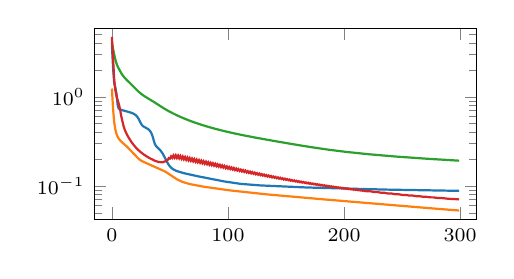
\begin{tikzpicture}

\definecolor{crimson2143940}{RGB}{214,39,40}
\definecolor{darkgray176}{RGB}{176,176,176}
\definecolor{darkorange25512714}{RGB}{255,127,14}
\definecolor{forestgreen4416044}{RGB}{44,160,44}
\definecolor{steelblue31119180}{RGB}{31,119,180}

\begin{axis}[compar,
	ymode=log]
\addplot [thick, steelblue31119180]
table {%
0 3.85001611709595
1 2.1458203792572
2 1.42304074764252
3 1.27057814598083
4 1.07568347454071
5 0.799212455749512
6 0.733221530914307
7 0.721283674240112
9 0.707787752151489
16 0.666974186897278
18 0.651615381240845
19 0.64179801940918
20 0.629560708999634
21 0.613784790039062
22 0.593032360076904
23 0.566002249717712
25 0.501725912094116
26 0.47937273979187
27 0.46651017665863
29 0.451001048088074
31 0.43555474281311
32 0.425134420394897
33 0.41105580329895
34 0.391023635864258
35 0.362361192703247
36 0.326099514961243
37 0.295191526412964
38 0.280576586723328
42 0.248737454414368
44 0.227878451347351
48 0.180903553962708
49 0.172060966491699
51 0.160104870796204
53 0.153125762939453
56 0.146742224693298
62 0.13903284072876
74 0.128426432609558
97 0.112231850624084
111 0.105488300323486
128 0.101377844810486
168 0.0961171388626099
235 0.0910736322402954
299 0.0881310701370239
};
\addplot [thick, darkorange25512714]
table {%
0 1.23822641372681
1 0.738285541534424
2 0.515761375427246
3 0.4292893409729
4 0.38191545009613
5 0.354934692382812
6 0.338408708572388
7 0.325846433639526
9 0.306785702705383
13 0.275501608848572
23 0.201859831809998
25 0.192705988883972
28 0.184560060501099
46 0.144832253456116
56 0.118885040283203
61 0.110710263252258
67 0.105042099952698
79 0.0981142520904541
101 0.0893926620483398
133 0.0805541276931763
184 0.0704268217086792
280 0.0554471015930176
299 0.0530545711517334
};
\addplot [thick, forestgreen4416044]
table {%
0 4.05598926544189
1 3.45300483703613
2 2.97763061523438
3 2.61971783638
4 2.35778474807739
5 2.18703508377075
6 2.06520247459412
7 1.95468974113464
8 1.84842002391815
9 1.76255404949188
10 1.69462144374847
11 1.63581776618958
12 1.58327627182007
13 1.53526997566223
14 1.49058413505554
16 1.40748488903046
21 1.20854544639587
22 1.17382073402405
23 1.14177072048187
24 1.11227011680603
25 1.08525025844574
26 1.06055045127869
28 1.01695835590363
30 0.978874087333679
33 0.927088260650635
37 0.862118482589722
44 0.752540469169617
46 0.725320339202881
49 0.689407587051392
52 0.657606840133667
55 0.628973245620728
59 0.595095992088318
63 0.565508365631104
67 0.539439916610718
72 0.510800004005432
77 0.485812664031982
83 0.459864139556885
89 0.437418222427368
96 0.414665579795837
104 0.392243146896362
113 0.370553493499756
124 0.347705125808716
138 0.322409272193909
155 0.295305252075195
171 0.273048043251038
186 0.255640983581543
202 0.240770101547241
221 0.226953506469727
244 0.213955640792847
273 0.201248288154602
299 0.192145466804504
};
\addplot [thick, crimson2143940]
table {%
0 4.69362020492554
1 2.7148494720459
2 1.54917848110199
3 1.17751252651215
4 1.0149405002594
5 0.90976893901825
6 0.828250408172607
7 0.726314544677734
8 0.61180305480957
9 0.536312222480774
10 0.472319364547729
11 0.429957985877991
12 0.400319814682007
13 0.376694202423096
14 0.356591105461121
15 0.338947892189026
17 0.309252738952637
19 0.285506248474121
21 0.266453266143799
23 0.251017570495605
26 0.232697129249573
29 0.218315958976746
33 0.203232884407043
37 0.191822648048401
40 0.185920238494873
43 0.184518098831177
44 0.184627890586853
45 0.187541604042053
46 0.188506722450256
47 0.194794178009033
48 0.195274114608765
49 0.205084681510925
50 0.202417969703674
51 0.214552879333496
52 0.206847906112671
53 0.219677567481995
54 0.207814335823059
55 0.220445871353149
56 0.206572294235229
57 0.218820691108704
58 0.204374670982361
59 0.216279745101929
60 0.201866745948792
61 0.213473916053772
62 0.199298739433289
63 0.210629820823669
64 0.196754813194275
65 0.207815408706665
66 0.194255113601685
67 0.205044865608215
68 0.191802024841309
69 0.202317833900452
70 0.189392685890198
71 0.199632048606873
72 0.187022805213928
73 0.196983456611633
74 0.184688091278076
75 0.194367408752441
76 0.182385087013245
77 0.191782355308533
78 0.180112361907959
79 0.189228415489197
80 0.177868366241455
81 0.186703562736511
82 0.175650596618652
83 0.184206366539001
84 0.173459053039551
85 0.181738138198853
86 0.171293258666992
87 0.179298281669617
88 0.169152617454529
89 0.176887392997742
90 0.167037963867188
91 0.174506902694702
92 0.16494882106781
93 0.172156095504761
94 0.162885546684265
95 0.169836640357971
96 0.160848617553711
97 0.167548418045044
98 0.158838629722595
99 0.165292978286743
100 0.156855821609497
101 0.163070917129517
102 0.154901623725891
103 0.160883188247681
104 0.15297532081604
105 0.158729791641235
106 0.15107786655426
107 0.156611561775208
108 0.149209976196289
109 0.154529452323914
110 0.147372007369995
111 0.152483701705933
112 0.145563960075378
113 0.150474071502686
114 0.143786668777466
115 0.148502349853516
116 0.142040610313416
117 0.146567940711975
118 0.140325665473938
119 0.144671440124512
120 0.138642072677612
121 0.14281153678894
122 0.136988997459412
123 0.140989542007446
124 0.135367751121521
125 0.139204740524292
126 0.133777260780334
127 0.137457251548767
128 0.132217884063721
129 0.135746121406555
130 0.130689024925232
131 0.134072184562683
132 0.129191517829895
133 0.132434606552124
134 0.127724409103394
135 0.130833268165588
136 0.126287460327148
137 0.129267334938049
138 0.124881029129028
139 0.127737283706665
140 0.123503923416138
141 0.126241326332092
142 0.122155427932739
143 0.124778866767883
144 0.120835781097412
145 0.123349666595459
146 0.11954402923584
147 0.12195360660553
148 0.118280410766602
149 0.120589852333069
150 0.117044448852539
151 0.119257688522339
152 0.115834832191467
153 0.117956519126892
154 0.114651560783386
155 0.116685271263123
156 0.113493919372559
157 0.115443706512451
158 0.112361907958984
159 0.11423134803772
160 0.111255049705505
161 0.113047957420349
162 0.110172152519226
163 0.111891508102417
164 0.109112620353699
165 0.110761642456055
166 0.108076214790344
167 0.109657764434814
168 0.107062339782715
169 0.108580470085144
170 0.106070995330811
171 0.107527494430542
172 0.105100989341736
173 0.106499433517456
174 0.10415244102478
175 0.105494618415833
176 0.103224039077759
177 0.104513049125671
178 0.102315545082092
179 0.103553533554077
180 0.101426720619202
181 0.102616190910339
182 0.100557088851929
183 0.101700305938721
184 0.0997061729431152
185 0.100804686546326
186 0.0988726615905762
187 0.0999287366867065
188 0.0980567932128906
189 0.0990729331970215
190 0.0972588062286377
191 0.0982364416122437
192 0.0964773893356323
193 0.097417950630188
194 0.0957117080688477
195 0.0966169834136963
196 0.0949617624282837
197 0.0958337783813477
198 0.0942277908325195
199 0.0950677394866943
200 0.0935087203979492
201 0.0943180322647095
202 0.0928041934967041
203 0.093584418296814
204 0.0921140909194946
205 0.0928663015365601
206 0.0914373397827148
207 0.0921628475189209
208 0.0907740592956543
209 0.091474175453186
210 0.0901238918304443
211 0.0907998085021973
212 0.089486837387085
213 0.090139627456665
214 0.0888618230819702
215 0.0894925594329834
216 0.0882493257522583
217 0.088858962059021
218 0.0876481533050537
220 0.0870583057403564
223 0.0870314836502075
226 0.085355281829834
229 0.0853092670440674
232 0.0837435722351074
235 0.0836825370788574
238 0.0822173357009888
241 0.082144021987915
244 0.0807691812515259
247 0.0806872844696045
250 0.0793938636779785
253 0.0793051719665527
256 0.0780863761901855
259 0.0779929161071777
262 0.0768417119979858
265 0.0767456293106079
268 0.0756555795669556
271 0.0755575895309448
274 0.0745236873626709
277 0.0744255781173706
280 0.0734424591064453
285 0.072994589805603
290 0.0717432498931885
295 0.0713222026824951
299 0.0706861019134521
};
\end{axis}

\end{tikzpicture}
}
	&
	\multicolumn{4}{c}{% This file was created with tikzplotlib v0.10.1.
\begin{tikzpicture}

\definecolor{crimson2143940}{RGB}{214,39,40}
\definecolor{darkgray176}{RGB}{176,176,176}
\definecolor{darkorange25512714}{RGB}{255,127,14}
\definecolor{forestgreen4416044}{RGB}{44,160,44}
\definecolor{steelblue31119180}{RGB}{31,119,180}

\begin{axis}[
height=\figheight,
tick align=outside,
tick pos=left,
width=\figwidth,
x grid style={darkgray176},
xmin=-0.95, xmax=19.95,
xtick style={color=black},
y grid style={darkgray176},
ymin=-2.57960711717606, ymax=31.5117500901222,
ytick style={color=black}
]
\addplot [semithick, steelblue31119180]
table {%
0 11.0500001907349
1 11.1800003051758
2 15.4399995803833
3 17.7099990844727
4 18.8500003814697
5 19.3099994659424
6 19.3700008392334
7 19.1599998474121
9 18.6399993896484
10 18.3899993896484
11 18.1599998474121
12 17.9599990844727
13 17.7999992370605
14 17.6700000762939
15 17.5599994659424
16 17.4699993133545
17 17.3999996185303
19 17.2999992370605
};
\addplot [semithick, darkorange25512714]
table {%
0 10.9399995803833
1 17.0499992370605
2 21.9500007629395
3 22.2999992370605
4 21.9200000762939
5 21.4899997711182
6 21.1499996185303
7 20.8999996185303
8 20.6800003051758
10 20.2800006866455
11 20.0400009155273
12 19.7099990844727
14 18.7700004577637
15 18.4400005340576
16 18.2399997711182
17 18.1000003814697
18 18.0200004577637
19 17.9599990844727
};
\addplot [semithick, forestgreen4416044]
table {%
0 -1.02999997138977
1 9
2 12.1800003051758
3 14.4300003051758
4 15.6499996185303
5 16.2800006866455
6 16.7199993133545
7 17.2399997711182
8 17.8999996185303
9 18.4400005340576
10 18.8500003814697
11 19.0400009155273
12 19.0799999237061
13 19
14 18.8400001525879
15 18.6299991607666
16 18.3799991607666
17 18.1399993896484
18 17.9400005340576
19 17.7999992370605
};
\addplot [semithick, crimson2143940]
table {%
0 5.19000005722046
1 10.2700004577637
2 13.2799997329712
3 14.5900001525879
4 15.2399997711182
5 15.5799999237061
6 15.9099998474121
7 16.1700000762939
8 16.3400001525879
9 16.4500007629395
10 16.5799999237061
11 16.6800003051758
12 16.6900005340576
13 16.6299991607666
14 16.5400009155273
15 16.4599990844727
16 16.4099998474121
17 16.3899993896484
18 16.3799991607666
19 16.3799991607666
};
\addplot [semithick, gray]
table {%
-0.95 29.9621429443359
19.95 29.9621429443359
};
\end{axis}

\end{tikzpicture}
}
\end{tabular}
	\caption{$d=800$, avec passe-base}
	\label{fig:LGDlat800-s}
\end{figure}

\begin{figure}[H]\centering
	\begin{tabular}{c c c c c c}
	Target  &  $(1)$  &  $(2)$  &  $(3)$   &  $(4)$
	
	\\
	
	\multirow{2}{0.3\textwidth}[0.122\textwidth]{\includegraphics[width=0.3\textwidth]{resultats/LGD/lats/lat-800-target-g.png}}
	&
	\includegraphics[width=0.15\textwidth]{resultats/LGD/lats/lat-800_1-init-pas=10.0_filtre=g-0.6.png}
	&
	\includegraphics[width=0.15\textwidth]{resultats/LGD/lats/lat-800_2-init-pas=10.0_filtre=g-0.6.png}
	&
	\includegraphics[width=0.15\textwidth]{resultats/LGD/lats/lat-800_3-init-pas=10.0_filtre=g-0.6.png}
	&
	\includegraphics[width=0.15\textwidth]{resultats/LGD/lats/lat-800_4-init-pas=10.0_filtre=g-0.6.png}
	
	\\
	
	
	&
	\includegraphics[width=0.15\textwidth]{resultats/LGD/lats/lat-800_1-guess-pas=10.0_filtre=g-0.6.png}
	&
	\includegraphics[width=0.15\textwidth]{resultats/LGD/lats/lat-800_2-guess-pas=10.0_filtre=g-0.6.png}
	&
	\includegraphics[width=0.15\textwidth]{resultats/LGD/lats/lat-800_3-guess-pas=10.0_filtre=g-0.6.png}
	&
	\includegraphics[width=0.15\textwidth]{resultats/LGD/lats/lat-800_4-guess-pas=10.0_filtre=g-0.6.png}
	
	\\ \\
	
	
	
	\multicolumn{2}{c}{Loss}  &  \multicolumn{4}{c}{PSNR{\color{white}bbbb}}
	
	\\
	
	\multicolumn{2}{c}{% This file was created with tikzplotlib v0.10.1.
\begin{tikzpicture}

\definecolor{crimson2143940}{RGB}{214,39,40}
\definecolor{darkgray176}{RGB}{176,176,176}
\definecolor{darkorange25512714}{RGB}{255,127,14}
\definecolor{forestgreen4416044}{RGB}{44,160,44}
\definecolor{steelblue31119180}{RGB}{31,119,180}

\begin{axis}[
height=\figheight,
tick align=outside,
tick pos=left,
width=\figwidth,
x grid style={darkgray176},
xmin=-0.95, xmax=19.95,
xtick style={color=black},
y grid style={darkgray176},
ymin=-0.547165866941214, ymax=15.0585420243442,
ytick style={color=black}
]
\addplot [semithick, steelblue31119180]
table {%
0 2.93553948402405
1 1.87434804439545
2 1.10162699222565
3 0.695515155792236
4 0.369987845420837
5 0.243139982223511
6 0.179080009460449
8 0.162184476852417
15 0.184467554092407
19 0.200243592262268
};
\addplot [semithick, darkorange25512714]
table {%
0 1.26624810695648
1 0.418554663658142
2 0.244757056236267
3 0.188532590866089
4 0.177584409713745
5 0.173996567726135
10 0.190012454986572
16 0.208758592605591
19 0.212993383407593
};
\addplot [semithick, forestgreen4416044]
table {%
0 14.3491916656494
1 3.53692412376404
2 2.17629098892212
3 1.30119788646698
4 0.828463077545166
5 0.442574858665466
6 0.278957962989807
7 0.191884636878967
8 0.172186493873596
9 0.162286520004272
15 0.176749229431152
19 0.193746089935303
};
\addplot [semithick, crimson2143940]
table {%
0 6.1989574432373
1 2.70222043991089
2 1.7502475976944
3 1.00837326049805
4 0.632613182067871
5 0.344910740852356
6 0.230880498886108
7 0.176201343536377
9 0.163307666778564
19 0.198582410812378
};
\end{axis}

\end{tikzpicture}
}
	&
	\multicolumn{4}{c}{% This file was created with tikzplotlib v0.10.1.
\begin{tikzpicture}

\definecolor{crimson2143940}{RGB}{214,39,40}
\definecolor{darkgray176}{RGB}{176,176,176}
\definecolor{darkorange25512714}{RGB}{255,127,14}
\definecolor{forestgreen4416044}{RGB}{44,160,44}
\definecolor{steelblue31119180}{RGB}{31,119,180}

\begin{axis}[
height=\figheight,
tick align=outside,
tick pos=left,
width=\figwidth,
x grid style={darkgray176},
xmin=-0.95, xmax=19.95,
xtick style={color=black},
y grid style={darkgray176},
ymin=-2.57960711717606, ymax=31.5117500901222,
ytick style={color=black}
]
\addplot [semithick, steelblue31119180]
table {%
0 11.3299999237061
1 14.5600004196167
2 18.4799995422363
3 21.3500003814697
4 24.9899997711182
5 26.6900005340576
6 27.5400009155273
7 27.7600002288818
8 27.8400001525879
9 27.8199996948242
10 27.7700004577637
11 27.6599998474121
12 27.5100002288818
13 27.3199996948242
16 26.6900005340576
17 26.5
18 26.3199996948242
19 26.1700000762939
};
\addplot [semithick, darkorange25512714]
table {%
0 10.9399995803833
1 22.8500003814697
2 25.7900009155273
3 27.0400009155273
4 27.4300003051758
5 27.5200004577637
6 27.4400005340576
7 27.3099994659424
8 27.1399993896484
9 26.9500007629395
11 26.5499992370605
12 26.3700008392334
13 26.2099990844727
14 26.0599994659424
15 25.9400005340576
16 25.8400001525879
17 25.7600002288818
18 25.6900005340576
19 25.6299991607666
};
\addplot [semithick, forestgreen4416044]
table {%
0 -1.02999997138977
1 10.1499996185303
2 13.5299997329712
3 17.3600006103516
4 20.2299995422363
5 24.0400009155273
6 26.1100006103516
7 27.2600002288818
8 27.6299991607666
9 27.75
10 27.7800006866455
11 27.7700004577637
12 27.7000007629395
13 27.5799999237061
14 27.4200000762939
15 27.2299995422363
18 26.6299991607666
19 26.4500007629395
};
\addplot [semithick, crimson2143940]
table {%
0 5.21000003814697
1 12.0100002288818
2 15.1099996566772
3 19.0200004577637
4 21.9400005340576
5 25.2000007629395
6 26.8199996948242
7 27.5
8 27.6599998474121
9 27.6900005340576
10 27.6200008392334
11 27.5300006866455
12 27.3899993896484
13 27.2299995422363
14 27.0499992370605
15 26.8600006103516
16 26.6800003051758
17 26.5100002288818
18 26.3500003814697
19 26.2000007629395
};
\addplot [semithick, gray]
table {%
-0.95 29.9621429443359
19.95 29.9621429443359
};
\end{axis}

\end{tikzpicture}
}
\end{tabular}
	\caption{$d=800$, sans passe-base}
	\label{fig:LGDlat800-g}
\end{figure}
\`A noter que sur la loss de la figure \figref{fig:LGD comp_size g} lees algorithmes stagnent ce qui sous entend que l'on se trouve dans des vallées (ou des crêtes). Problème qui peut être évité en ajoutant de l'inertie à la descente avec des méthodes type heavy-ball ou Nesterof. 





\newpage



\section{Comparaison avec la descente de gradient projetée}\label{sec:comparPGD}

\subsection{Le principe et les résultats}\label{sec:PGD}
\quad 

La descente de gradient projeté par auto-encodeur était sensé faire office d'algorithme de contrôle. Comme son nom l'indique, la descente de gradient projeté (PGD) consiste en une descente de gradient classique à cela près qu'à itération, le vecteur obtenu est projeté par une fonction$f$ (voir \figref{fig:pcode PGD} ci-contre). 

\begin{wrapfigure}[17]{r}{0.38\textwidth}
    \fbox{\begin{minipage}{18em}
\vspace{0.3cm}
\begin{algorithmic}[0]
    \State $x_0$ : initialisation
    \State $x$ : image à reconstruire
    \State $\rho$ : pas de descente
    \State $N$ : nombre d'itération
    \State $y\ \ll\ A(x)$
    \State
    \For{$n\in \llbracket1,N-1\rrbracket$}
        \State $\nabla F(x_n)\ \ll\ ^tA\big(Ax_n-y_0\big)$
        \State $\ \ x_{n+1}\quad  \ll\ p\big(x_n\ - \rho \nabla F(x_n)\big)$
        \EndFor
    \State
    \Return $(x_n)_{0\leq n\leq N}$
\end{algorithmic}
\vspace{0.2cm}
\end{minipage}}
    \caption{Algorithme de PGD}
    \label{fig:pcode PGD}
\end{wrapfigure}
\noindent Dans notre cas, $f$ est un auto-encoder dont on notera $f_E$ et $f_D$ les parties encodage et décodage respectivement, de sorte que :
\[f = f_D\circ f_E\]{\color{white}l}
\\
Cette méthode est tirée de l'article \cite{peng_solving_2019} de P. Peng, S. Jalali and X. Yuan, et leurs résultats étaient satisfaisant. Pourtant comme on va le voir dans la section \ref{sec:res PGD} plus bas, nous n'avons pas réussi à les reproduire.
Cela étant dit, nous allons malgré tout détailler l'algorithme et essayer de comprendre les résultats obtenus.
\\
Ce rapport étant surtout porté sur la descente de gradient depuis l'espace lattent de $f$, on ne détaillera pas les arguments mathématiques qui supportent cette méthode mais on peut tout de même essayer de se convaincre de l'intérêt de la PGD.\\
Comme expliqué plus haut, le problème est convexe ce qui assure la convergence de la descente de gradient. La difficulté étant de tomber sur le bon argmin. C'est là que composer par $f$ peut aider à diriger la descente vers le ``bon'' minimum.


\begin{itemize}
	\item Converge beaucoup plus vite
	\item Sensible à l'excès d'itérations (sûrement parce que $f$ n'est pas une vrai identité, c'est un problème classique)
	\item Très sensible au pas image-wise
	\item Robuste à l'initialisation
\end{itemize}
%\\ \\



\subsection{Comparaison avec la LGD}\label{sec:res PGD}
\begin{figure}[H]\centering
    %\input{figures/PGD/PGD 2-s}
    \caption{Résultat de la PGD avec un pas de descente $\rho=10^{-10}$, sans passe-bas}
\end{figure}

\begin{figure}[H]\centering
    %\begin{tabular}{c c c}

Image cible $\bf{x_0}$  &  Image reconstruite par PGD  &  Évolution de $F$

\\

\includegraphics[width=0.25\textwidth]{resultats (legacy)/PGD/seed21-target-pas=1e-10_filtre=g-0.6.png}
&
\includegraphics[width=0.25\textwidth]{resultats (legacy)/PGD/seed21-guess-pas=1e-10_filtre=g-0.6.png}&
% This file was created with tikzplotlib v0.10.1.
\begin{tikzpicture}

\definecolor{darkgray176}{RGB}{176,176,176}

\begin{axis}[
height=\figheight,
tick align=outside,
tick pos=left,
width=\figwidth,
x grid style={darkgray176},
xmin=-14.95, xmax=313.95,
xtick style={color=black},
y grid style={darkgray176},
ymin=3.33846267461777, ymax=4.27462569475174,
ytick style={color=black}
]
\addplot [semithick, blue]
table {%
0 3.38101553916931
1 3.92825508117676
2 4.2053689956665
3 4.2320728302002
4 4.1864185333252
5 4.11872434616089
6 4.09811353683472
7 4.09209442138672
8 4.09062051773071
9 4.08995199203491
10 4.08711194992065
12 4.08036422729492
13 4.07745313644409
14 4.07500076293945
15 4.07309627532959
16 4.07194423675537
17 4.07178068161011
18 4.07246017456055
21 4.07559776306152
23 4.07689714431763
25 4.07709217071533
29 4.07682323455811
32 4.07738208770752
36 4.07902431488037
40 4.08074569702148
43 4.08150815963745
48 4.08195686340332
61 4.08205604553223
299 4.08205652236938
};
\end{axis}

\end{tikzpicture}


\\ \\

Image cible compressée $A(\bf{x_0})$  &  Initialisation de la PGD  & Évolution de PSNR

\\

\includegraphics[width=0.25\textwidth]{resultats (legacy)/PGD/seed21-comptarg-pas=1e-10_filtre=g-0.6.png}
&
\includegraphics[width=0.25\textwidth]{resultats (legacy)/PGD/seed21-init-pas=1e-10_filtre=g-0.6.png}
&
% This file was created with tikzplotlib v0.10.1.
\begin{tikzpicture}

\definecolor{darkgray176}{RGB}{176,176,176}
\definecolor{orange}{RGB}{255,165,0}

\begin{axis}[
height=\figheight,
tick align=outside,
tick pos=left,
width=\figwidth,
x grid style={darkgray176},
xmin=-14.95, xmax=313.95,
xtick style={color=black},
y grid style={darkgray176},
ymin=8.80650033950806, ymax=10.6435004234314,
ytick style={color=black}
]
\addplot [semithick, orange]
table {%
0 10.5600004196167
1 9.5600004196167
2 9
3 8.9399995803833
4 9.01000022888184
5 9.06999969482422
6 9.07999992370605
7 9.07999992370605
8 9.06999969482422
9 9.05000019073486
12 9.05000019073486
18 8.98999977111816
19 8.97000026702881
20 8.97000026702881
24 8.93000030517578
26 8.93000030517578
27 8.92000007629395
30 8.92000007629395
31 8.90999984741211
35 8.90999984741211
36 8.89999961853027
39 8.89999961853027
40 8.89000034332275
299 8.89000034332275
};
\end{axis}

\end{tikzpicture}


\end{tabular}
    \caption{Résultat de la PGD avec un pas de descente $\rho=10^{-10}$, passe-bas gaussien ($\sigma=0.6$)}
\end{figure}

\begin{figure}[H]\centering
    %\begin{tabular}{c c c c c c c}
Target  &  $(1)$  &  $(2)$  &  $(3)$  &  $(4)$  &  $(5)$  &  $(6)$

\\

\includegraphics[width=0.12\textwidth]{resultats (legacy)/PGD/comp-pas-s1-target-pas=0.01_filtre=s-None.png}
&
\includegraphics[width=0.12\textwidth]{resultats (legacy)/PGD/comp-pas-s1_1-guess-pas=1.1_filtre=s-None.png}
&
\includegraphics[width=0.12\textwidth]{resultats (legacy)/PGD/comp-pas-s1_2-guess-pas=0.9_filtre=s-None.png}
&
\includegraphics[width=0.12\textwidth]{resultats (legacy)/PGD/comp-pas-s1_3-guess-pas=0.7_filtre=s-None.png}
&
\includegraphics[width=0.12\textwidth]{resultats (legacy)/PGD/comp-pas-s1_4-guess-pas=0.5_filtre=s-None.png}
&
\includegraphics[width=0.12\textwidth]{resultats (legacy)/PGD/comp-pas-s1_5-guess-pas=0.1_filtre=s-None.png}
&
\includegraphics[width=0.12\textwidth]{resultats (legacy)/PGD/comp-pas-s1_6-guess-pas=0.01_filtre=s-None.png}

\\
&  $\rho=1.1$  &  $\rho=0.9$  &  $\rho=0.7$  &  $\rho=0.5$  &  $\rho=0.1$  &  $\rho=0.01$

\\ \\


\multicolumn{3}{c}{\quad Évolution des loss}
&
\multicolumn{3}{c}{\qquad\qquad Évolution des PSNR}

\\

\multicolumn{3}{c}{% This file was created with tikzplotlib v0.10.1.
\begin{tikzpicture}

\definecolor{crimson2143940}{RGB}{214,39,40}
\definecolor{darkgray176}{RGB}{176,176,176}
\definecolor{darkorange25512714}{RGB}{255,127,14}
\definecolor{forestgreen4416044}{RGB}{44,160,44}
\definecolor{mediumpurple148103189}{RGB}{148,103,189}
\definecolor{sienna1408675}{RGB}{140,86,75}
\definecolor{steelblue31119180}{RGB}{31,119,180}

\begin{axis}[
height=\figheight,
tick align=outside,
tick pos=left,
width=\figwidth,
x grid style={darkgray176},
xmin=-4.95, xmax=103.95,
xtick style={color=black},
y grid style={darkgray176},
ymin=-0.264805173873901, ymax=5.56090865135193,
ytick style={color=black}
]
\addplot [semithick, steelblue31119180]
table {%
0 0
1 4.07896375656128
2 3.52517080307007
3 3.12815141677856
4 2.81518316268921
5 2.56268668174744
6 2.41218519210815
7 2.32254910469055
8 2.24398493766785
9 2.1550874710083
10 2.04974150657654
11 1.94149577617645
12 1.85119020938873
13 1.78053987026215
14 1.72163999080658
16 1.61274838447571
17 1.55523943901062
18 1.49298596382141
19 1.4247362613678
20 1.35008704662323
21 1.27169048786163
22 1.19849848747253
23 1.14036464691162
24 1.09690809249878
25 1.06362283229828
26 1.03781700134277
27 1.01737356185913
28 1.00106072425842
29 0.98879337310791
30 0.980517625808716
33 0.965440154075623
35 0.957900524139404
36 0.957945704460144
37 0.962774991989136
38 0.972147226333618
46 1.06584620475769
50 1.11546194553375
52 1.1362316608429
54 1.15210509300232
56 1.16279006004333
58 1.16916263103485
61 1.1736353635788
66 1.17550802230835
90 1.17538797855377
99 1.17537343502045
};
\addplot [semithick, darkorange25512714]
table {%
0 0
1 4.07896375656128
2 3.68217897415161
3 3.41303467750549
4 3.27746367454529
5 3.16378164291382
6 3.05855870246887
7 2.96412682533264
8 2.89624261856079
9 2.85797500610352
10 2.83769059181213
11 2.82628059387207
12 2.82035517692566
13 2.81888937950134
14 2.82101798057556
18 2.83915281295776
20 2.839919090271
24 2.83509492874146
25 2.8367612361908
26 2.84170770645142
27 2.85064959526062
31 2.89562010765076
34 2.92370295524597
35 2.93018984794617
36 2.93084073066711
37 2.92324113845825
38 2.90725541114807
39 2.88498115539551
42 2.81203198432922
43 2.79147887229919
44 2.77665281295776
45 2.7579562664032
46 2.71232795715332
47 2.63271260261536
48 2.51651525497437
49 2.37964010238647
50 2.26284599304199
51 2.18112254142761
52 2.12654852867126
53 2.08971452713013
54 2.06392884254456
55 2.04536175727844
56 2.03200602531433
57 2.02255630493164
59 2.01067805290222
60 2.00684094429016
61 2.00561332702637
62 2.00979232788086
64 2.02727031707764
65 2.03128576278687
66 2.0311872959137
68 2.02385687828064
71 2.00536942481995
75 1.9788613319397
78 1.96282684803009
83 1.94115149974823
89 1.91430306434631
93 1.89214110374451
96 1.87565422058105
99 1.86520540714264
};
\addplot [semithick, forestgreen4416044]
table {%
0 0
1 4.07896375656128
2 3.8205451965332
3 3.62880373001099
4 3.59577369689941
5 3.57894825935364
7 3.52864384651184
9 3.47441124916077
10 3.44589066505432
11 3.41447138786316
12 3.37740063667297
13 3.3326997756958
14 3.28390336036682
15 3.2418737411499
16 3.21481728553772
17 3.20173120498657
18 3.19775176048279
19 3.19886231422424
21 3.2087984085083
22 3.2165834903717
23 3.22645115852356
24 3.23891043663025
25 3.25468277931213
26 3.27456378936768
27 3.29879713058472
30 3.37813758850098
36 3.51523613929749
37 3.52785992622375
38 3.53350329399109
42 3.542884349823
43 3.54671359062195
44 3.54803013801575
46 3.53936624526978
47 3.54797315597534
48 3.57345414161682
49 3.5877788066864
50 3.58951210975647
51 3.58553290367126
55 3.56243348121643
58 3.55092120170593
59 3.54289412498474
60 3.5255331993103
61 3.49262976646423
62 3.45118856430054
63 3.42291903495789
64 3.40627121925354
68 3.35461449623108
70 3.33442378044128
72 3.32210063934326
74 3.31670355796814
76 3.31729507446289
77 3.32043409347534
78 3.32643532752991
79 3.3359112739563
81 3.36291480064392
83 3.39171957969666
85 3.41468930244446
87 3.43023324012756
89 3.44056844711304
91 3.44824767112732
93 3.45331287384033
94 3.46086668968201
95 3.45691871643066
96 3.44251346588135
97 3.42187762260437
98 3.39602041244507
99 3.36537027359009
};
\addplot [semithick, crimson2143940]
table {%
0 0
1 4.07896375656128
2 3.94823622703552
3 3.80108308792114
4 3.78965187072754
5 3.79547238349915
6 3.78107476234436
8 3.7436625957489
9 3.72878503799438
10 3.71715617179871
11 3.70839047431946
12 3.70217561721802
13 3.69829487800598
15 3.69651627540588
19 3.70093441009521
21 3.69738125801086
24 3.69032216072083
26 3.69020771980286
36 3.70123338699341
37 3.70583987236023
38 3.71418929100037
39 3.72724795341492
42 3.77587366104126
43 3.78566789627075
44 3.79075264930725
45 3.79218196868896
47 3.78928422927856
52 3.77963805198669
74 3.74674415588379
82 3.74110007286072
91 3.73915147781372
98 3.74113392829895
99 3.74187564849854
};
\addplot [semithick, mediumpurple148103189]
table {%
0 0
1 4.07896375656128
2 4.20143127441406
3 4.18282270431519
4 4.07413816452026
5 4.01319360733032
6 4.0098295211792
8 4.00828313827515
10 3.9943208694458
11 3.99805307388306
13 4.03817749023438
14 4.04082536697388
15 4.03497409820557
16 4.03643465042114
19 4.04919767379761
20 4.05767297744751
21 4.07760524749756
22 4.11900758743286
23 4.18120098114014
24 4.25132083892822
25 4.3161096572876
26 4.33346223831177
27 4.35759210586548
28 4.41550207138062
29 4.46173143386841
30 4.48590850830078
31 4.49872064590454
33 4.51173448562622
35 4.52376794815063
36 4.53285932540894
37 4.54655408859253
38 4.56601190567017
39 4.58160257339478
40 4.58052206039429
42 4.55558919906616
43 4.55141973495483
45 4.55555009841919
46 4.55513620376587
50 4.5451512336731
51 4.55182218551636
52 4.56834697723389
53 4.59388399124146
54 4.60153150558472
57 4.56292104721069
59 4.54803514480591
60 4.54122066497803
61 4.53067779541016
62 4.50368785858154
63 4.4599347114563
64 4.43334245681763
65 4.42784452438354
66 4.43072175979614
67 4.43723678588867
68 4.44729900360107
69 4.46444177627563
70 4.55684423446655
71 4.63702630996704
72 4.70514965057373
74 4.59016847610474
75 4.57998275756836
76 4.61408805847168
77 4.67671489715576
78 4.75459003448486
79 4.75405120849609
80 4.71129560470581
81 4.75442266464233
82 4.78543329238892
83 4.79236507415771
84 4.78348731994629
85 4.75929403305054
86 4.74150371551514
87 4.74146127700806
88 4.75127363204956
89 4.80999851226807
90 4.82527351379395
91 4.76644897460938
92 4.69950532913208
93 4.6431303024292
94 4.64853620529175
95 4.67958164215088
96 4.75133943557739
97 4.85158443450928
98 4.90142774581909
99 4.90428638458252
};
\addplot [semithick, sienna1408675]
table {%
0 0
1 4.07896375656128
2 4.26257085800171
3 4.29840040206909
4 4.31559228897095
5 4.29680633544922
6 4.28421878814697
7 4.26799869537354
10 4.20488739013672
11 4.19218683242798
12 4.20002508163452
13 4.2350492477417
14 4.2576265335083
15 4.26918935775757
16 4.27773427963257
17 4.28240823745728
18 4.29785299301147
19 4.35661697387695
21 4.49404048919678
23 4.59406995773315
24 4.62606239318848
25 4.63771677017212
26 4.66309595108032
27 4.6948127746582
28 4.69933652877808
30 4.68756246566772
31 4.67648220062256
32 4.660475730896
33 4.64902544021606
34 4.65869140625
35 4.67483520507812
37 4.69446039199829
38 4.67967176437378
39 4.61586284637451
40 4.57644414901733
41 4.58235645294189
42 4.61419677734375
43 4.62959957122803
44 4.61973333358765
45 4.60397577285767
48 4.56872510910034
49 4.5660080909729
50 4.57988357543945
51 4.61799669265747
52 4.73879051208496
53 4.79972267150879
54 4.75632619857788
55 4.76513814926147
56 4.82943058013916
58 5.09398937225342
59 5.20115375518799
60 5.29610347747803
61 5.24005365371704
62 5.13516235351562
63 5.0555944442749
64 4.96172857284546
65 4.83070421218872
66 4.84230327606201
67 4.92264270782471
68 4.98552894592285
69 4.98272562026978
70 4.90815019607544
71 4.87900400161743
72 4.81329298019409
73 4.73470258712769
74 4.70453357696533
75 4.69143533706665
76 4.68353652954102
77 4.68474006652832
78 4.69263648986816
80 4.71166610717773
81 4.714515209198
82 4.70982027053833
84 4.69606494903564
85 4.70591306686401
86 4.73970317840576
87 4.79891109466553
88 4.86688661575317
89 4.91673183441162
90 4.93967008590698
91 4.94825172424316
93 4.95826292037964
94 4.96681976318359
96 4.99044322967529
97 4.9943642616272
98 4.98428583145142
99 4.96689653396606
};
\end{axis}

\end{tikzpicture}
}
&
\multicolumn{4}{c}{% This file was created with tikzplotlib v0.10.1.
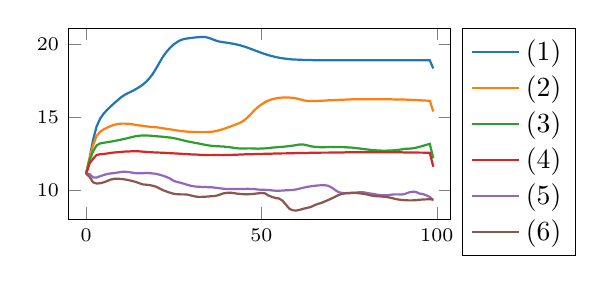
\begin{tikzpicture}

\definecolor{crimson2143940}{RGB}{214,39,40}
\definecolor{darkgray176}{RGB}{176,176,176}
\definecolor{darkorange25512714}{RGB}{255,127,14}
\definecolor{forestgreen4416044}{RGB}{44,160,44}
\definecolor{mediumpurple148103189}{RGB}{148,103,189}
\definecolor{sienna1408675}{RGB}{140,86,75}
\definecolor{steelblue31119180}{RGB}{31,119,180}

\begin{axis}[compar, legend pos=outer north east]
\addplot [thick, steelblue31119180]
table {%
0 11.1400003433228
1 12.1999998092651
2 13.460000038147
3 14.3699998855591
4 14.8999996185303
5 15.2399997711182
6 15.5
7 15.7299995422363
8 15.9499998092651
9 16.1599998474121
10 16.3600006103516
11 16.5200004577637
12 16.6499996185303
13 16.7600002288818
14 16.8899993896484
15 17.0300006866455
16 17.1900005340576
17 17.3899993896484
18 17.6399993896484
19 17.9500007629395
20 18.3400001525879
21 18.7600002288818
22 19.1599998474121
23 19.4799995422363
24 19.75
25 19.9699993133545
26 20.1399993896484
27 20.2700004577637
28 20.3400001525879
29 20.3799991607666
31 20.4400005340576
33 20.4799995422363
34 20.4699993133545
35 20.4099998474121
37 20.2299995422363
38 20.1599998474121
39 20.1200008392334
40 20.0900001525879
42 20.0100002288818
43 19.9599990844727
44 19.8999996185303
45 19.8299999237061
46 19.75
50 19.3899993896484
52 19.2299995422363
54 19.1100006103516
55 19.0599994659424
56 19.0200004577637
58 18.9599990844727
59 18.9400005340576
63 18.8999996185303
64 18.8999996185303
65 18.8899993896484
69 18.8899993896484
70 18.8799991607666
98 18.8799991607666
99 18.3299999237061
};
\addlegendentry{$(1)$}
\addplot [thick, darkorange25512714]
table {%
0 11.1400003433228
1 12.1999998092651
2 13.1000003814697
3 13.7200002670288
4 14.0100002288818
5 14.1700000762939
7 14.3900003433228
8 14.4799995422363
9 14.5299997329712
10 14.5600004196167
11 14.5600004196167
12 14.5500001907349
13 14.5200004577637
15 14.4399995803833
18 14.3500003814697
20 14.3100004196167
21 14.2799997329712
23 14.1999998092651
24 14.1700000762939
26 14.0900001525879
28 14.0299997329712
29 14.0100002288818
32 13.9799995422363
34 13.9799995422363
35 13.9899997711182
36 14.0100002288818
37 14.0500001907349
38 14.1099996566772
39 14.1800003051758
40 14.2600002288818
43 14.5299997329712
44 14.6300001144409
45 14.7700004577637
46 14.9700002670288
48 15.4700002670288
49 15.6899995803833
50 15.8699998855591
51 16.0200004577637
52 16.1399993896484
53 16.2199993133545
54 16.2800006866455
55 16.3199996948242
56 16.3400001525879
57 16.3500003814697
58 16.3400001525879
59 16.3199996948242
60 16.2800006866455
61 16.2199993133545
62 16.1499996185303
63 16.1100006103516
64 16.1000003814697
65 16.1000003814697
68 16.1299991607666
69 16.1499996185303
76 16.2199993133545
77 16.2199993133545
78 16.2299995422363
84 16.2299995422363
85 16.2199993133545
87 16.2199993133545
88 16.2099990844727
90 16.2099990844727
95 16.1599998474121
96 16.1399993896484
98 16.1200008392334
99 15.3900003433228
};
\addlegendentry{$(2)$}
\addplot [thick, forestgreen4416044]
table {%
0 11.1400003433228
1 12.0799999237061
2 12.6700000762939
3 13.0699996948242
4 13.210000038147
8 13.3699998855591
11 13.5200004577637
13 13.6400003433228
14 13.6899995803833
15 13.7299995422363
16 13.75
17 13.75
18 13.7399997711182
22 13.6599998474121
23 13.6300001144409
24 13.6099996566772
25 13.5699996948242
26 13.5200004577637
29 13.3400001525879
30 13.3000001907349
31 13.25
32 13.210000038147
34 13.1099996566772
35 13.0699996948242
36 13.039999961853
37 13.0200004577637
39 13
40 12.9700002670288
41 12.9499998092651
42 12.9099998474121
43 12.8800001144409
44 12.8599996566772
45 12.8599996566772
46 12.8699998855591
47 12.8699998855591
49 12.8500003814697
51 12.8699998855591
52 12.8900003433228
53 12.9200000762939
57 13
59 13.0600004196167
61 13.1400003433228
62 13.1300001144409
63 13.0799999237061
64 13.0200004577637
65 12.9799995422363
66 12.960000038147
67 12.9499998092651
68 12.9499998092651
69 12.960000038147
73 12.960000038147
74 12.9499998092651
75 12.9300003051758
76 12.9200000762939
81 12.7700004577637
83 12.7299995422363
85 12.710000038147
88 12.7399997711182
90 12.8000001907349
91 12.8400001525879
92 12.8500003814697
93 12.8699998855591
94 12.9099998474121
95 12.9700002670288
98 13.1800003051758
99 12.1899995803833
};
\addlegendentry{$(3)$}
\addplot [thick, crimson2143940]
table {%
0 11.1400003433228
1 11.8500003814697
2 12.1700000762939
3 12.4200000762939
4 12.4700002670288
5 12.4899997711182
6 12.5200004577637
7 12.5600004196167
8 12.5900001525879
11 12.6499996185303
14 12.6800003051758
15 12.6700000762939
17 12.6300001144409
18 12.6199998855591
19 12.6000003814697
23 12.5600004196167
24 12.539999961853
26 12.5200004577637
27 12.5
29 12.4799995422363
30 12.460000038147
32 12.4399995803833
33 12.4200000762939
34 12.4200000762939
35 12.4099998474121
36 12.4099998474121
37 12.4200000762939
38 12.4099998474121
39 12.4099998474121
40 12.4200000762939
41 12.4200000762939
46 12.4700002670288
47 12.4700002670288
49 12.4899997711182
50 12.4899997711182
52 12.5100002288818
53 12.5100002288818
54 12.5200004577637
55 12.5200004577637
56 12.5299997329712
57 12.5299997329712
58 12.539999961853
59 12.539999961853
60 12.5500001907349
61 12.5500001907349
62 12.5600004196167
63 12.5600004196167
64 12.5699996948242
66 12.5699996948242
67 12.5799999237061
69 12.5799999237061
70 12.5900001525879
73 12.5900001525879
74 12.6000003814697
90 12.6000003814697
91 12.5900001525879
94 12.5900001525879
95 12.5799999237061
96 12.5799999237061
97 12.5699996948242
98 12.5699996948242
99 11.6199998855591
};
\addlegendentry{$(4)$}
\addplot [thick, mediumpurple148103189]
table {%
0 11.1400003433228
1 11.1199998855591
2 10.8900003433228
3 10.8800001144409
4 10.9700002670288
5 11.0500001907349
6 11.1199998855591
7 11.1599998474121
8 11.1800003051758
10 11.2600002288818
11 11.2799997329712
12 11.2600002288818
14 11.1800003051758
15 11.1700000762939
16 11.1700000762939
17 11.1899995803833
18 11.1800003051758
19 11.1599998474121
20 11.1300001144409
21 11.0699996948242
22 11
23 10.9099998474121
24 10.8000001907349
25 10.6499996185303
26 10.5699996948242
27 10.5200004577637
28 10.4499998092651
29 10.3699998855591
30 10.3100004196167
31 10.2700004577637
32 10.25
36 10.210000038147
39 10.1199998855591
40 10.1000003814697
41 10.0900001525879
43 10.0900001525879
44 10.1000003814697
45 10.1000003814697
46 10.1099996566772
48 10.0900001525879
49 10.0600004196167
50 10.039999961853
51 10.039999961853
52 10.0299997329712
53 10
54 9.97999954223633
55 9.97999954223633
56 9.98999977111816
57 10.0100002288818
59 10.0299997329712
60 10.0699996948242
62 10.1899995803833
63 10.2399997711182
64 10.2799997329712
66 10.3400001525879
68 10.3599996566772
69 10.3199996948242
70 10.1999998092651
71 10.0299997329712
72 9.88000011444092
73 9.82999992370605
74 9.80000019073486
76 9.81999969482422
78 9.88000011444092
79 9.88000011444092
80 9.82999992370605
81 9.78999996185303
82 9.76000022888184
83 9.71000003814697
84 9.68000030517578
85 9.67000007629395
86 9.67000007629395
87 9.71000003814697
88 9.72999954223633
89 9.72999954223633
90 9.72000026702881
91 9.77000045776367
92 9.85999965667725
93 9.90999984741211
94 9.89999961853027
95 9.78999996185303
96 9.75
97 9.67000007629395
98 9.55000019073486
99 9.30000019073486
};
\addlegendentry{$(5)$}
\addplot [thick, sienna1408675]
table {%
0 11.1400003433228
1 10.9200000762939
2 10.5500001907349
3 10.4700002670288
4 10.4899997711182
5 10.5500001907349
6 10.6400003433228
7 10.7399997711182
8 10.789999961853
9 10.8000001907349
10 10.7799997329712
11 10.75
12 10.710000038147
14 10.5900001525879
15 10.5100002288818
16 10.4200000762939
17 10.3900003433228
18 10.3699998855591
19 10.3199996948242
20 10.25
22 10.0100002288818
23 9.92000007629395
24 9.84000015258789
25 9.77000045776367
26 9.73999977111816
27 9.72999954223633
28 9.72999954223633
29 9.71000003814697
31 9.59000015258789
32 9.5600004196167
33 9.5600004196167
34 9.56999969482422
37 9.63000011444092
38 9.69999980926514
39 9.78999996185303
40 9.82999992370605
41 9.85000038146973
42 9.81999969482422
43 9.77999973297119
45 9.73999977111816
46 9.73999977111816
47 9.75
48 9.77000045776367
49 9.80000019073486
50 9.81999969482422
51 9.80000019073486
52 9.64999961853027
53 9.5600004196167
54 9.47999954223633
55 9.44999980926514
56 9.30000019073486
58 8.73999977111816
59 8.64000034332275
60 8.63000011444092
61 8.68000030517578
62 8.75
63 8.8100004196167
64 8.85999965667725
65 8.97999954223633
66 9.06999969482422
67 9.14000034332275
69 9.34000015258789
70 9.44999980926514
72 9.6899995803833
73 9.76000022888184
74 9.8100004196167
75 9.82999992370605
76 9.84000015258789
77 9.82999992370605
79 9.77000045776367
80 9.72999954223633
81 9.67000007629395
82 9.61999988555908
83 9.60000038146973
84 9.59000015258789
85 9.56999969482422
86 9.53999996185303
87 9.48999977111816
88 9.43000030517578
89 9.38000011444092
90 9.35000038146973
91 9.32999992370605
92 9.31999969482422
93 9.31999969482422
94 9.32999992370605
95 9.35999965667725
96 9.38000011444092
98 9.39999961853027
99 9.39999961853027
};
\addlegendentry{$(6)$}
\end{axis}

\end{tikzpicture}
}
\end{tabular}
    \caption{Comparaison de la PGD avec le résultat attendu (Target) après 100 itérations et avec différent pas --- initialisation $^tA(Ax)$, sans passe-bas}
\end{figure}

\begin{figure}[H]\centering
    %\begin{tabular}{c c c c c c c}
Target  &  $(1)$  &  $(2)$  &  $(3)$  &  $(4)$  &  $(5)$  &  $(6)$

\\

\includegraphics[width=0.12\textwidth]{resultats (legacy)/PGD/comp-pas-g1-target-pas=0.5_filtre=g-0.5.png}
&
\includegraphics[width=0.12\textwidth]{resultats (legacy)/PGD/comp-pas-g1_1-guess-pas=1.1_filtre=g-0.5.png}
&
\includegraphics[width=0.12\textwidth]{resultats (legacy)/PGD/comp-pas-g1_2-guess-pas=0.9_filtre=g-0.5.png}
&
\includegraphics[width=0.12\textwidth]{resultats (legacy)/PGD/comp-pas-g1_3-guess-pas=0.7_filtre=g-0.5.png}
&
\includegraphics[width=0.12\textwidth]{resultats (legacy)/PGD/comp-pas-g1_4-guess-pas=0.5_filtre=g-0.5.png}
&
\includegraphics[width=0.12\textwidth]{resultats (legacy)/PGD/comp-pas-g1_5-guess-pas=0.1_filtre=g-0.5.png}
&
\includegraphics[width=0.12\textwidth]{resultats (legacy)/PGD/comp-pas-g1_6-guess-pas=0.01_filtre=g-0.5.png}

\\

&  $\rho=1.1$  &  $\rho=0.9$  &  $\rho=0.7$  &  $\rho=0.5$  &  $\rho=0.1$  &  $\rho=0.01$

\\ \\


\multicolumn{3}{c}{\quad Évolution des loss}
&
\multicolumn{3}{c}{\qquad\qquad Évolution des PSNR}

\\

\multicolumn{3}{c}{% This file was created with tikzplotlib v0.10.1.
\begin{tikzpicture}

\definecolor{crimson2143940}{RGB}{214,39,40}
\definecolor{darkgray176}{RGB}{176,176,176}
\definecolor{darkorange25512714}{RGB}{255,127,14}
\definecolor{forestgreen4416044}{RGB}{44,160,44}
\definecolor{mediumpurple148103189}{RGB}{148,103,189}
\definecolor{sienna1408675}{RGB}{140,86,75}
\definecolor{steelblue31119180}{RGB}{31,119,180}

\begin{axis}[
height=\figheight,
tick align=outside,
tick pos=left,
width=\figwidth,
x grid style={darkgray176},
xmin=-4.95, xmax=103.95,
xtick style={color=black},
y grid style={darkgray176},
ymin=2.27105427980423, ymax=4.27701591253281,
ytick style={color=black}
]
\addplot [semithick, steelblue31119180]
table {%
0 3.11796808242798
1 3.15118432044983
2 3.01552939414978
3 2.84774732589722
4 2.75995588302612
5 2.73878240585327
6 2.73351860046387
7 2.72573399543762
8 2.71427464485168
9 2.70477652549744
10 2.70237755775452
11 2.70297002792358
12 2.69900965690613
13 2.68789911270142
14 2.67062258720398
15 2.64913964271545
16 2.62546396255493
17 2.59937429428101
18 2.57031655311584
20 2.50738406181335
21 2.4793426990509
22 2.4574179649353
23 2.44052267074585
24 2.42700123786926
25 2.41591334342957
26 2.40676498413086
27 2.39922213554382
28 2.39300632476807
29 2.38787364959717
30 2.38361406326294
32 2.37704825401306
34 2.37229657173157
36 2.36874318122864
39 2.36492252349854
42 2.36257195472717
44 2.36234927177429
45 2.36335945129395
46 2.36629676818848
47 2.37319493293762
48 2.38594627380371
49 2.40138411521912
50 2.41227293014526
51 2.41700339317322
52 2.41823697090149
54 2.41712141036987
55 2.41559243202209
56 2.41324472427368
58 2.40651035308838
60 2.39966654777527
62 2.39470195770264
64 2.39169883728027
66 2.3901059627533
69 2.38922643661499
75 2.38944745063782
99 2.39285945892334
};
\addplot [semithick, darkorange25512714]
table {%
0 3.11796808242798
1 3.32535791397095
2 3.3224675655365
3 3.23482942581177
4 3.13118267059326
5 3.0477180480957
6 2.99429082870483
7 2.96304988861084
8 2.94067072868347
9 2.92288279533386
10 2.91210031509399
11 2.90701508522034
12 2.90518188476562
15 2.90581560134888
16 2.90258741378784
17 2.89445948600769
18 2.8795325756073
19 2.85680174827576
21 2.8011839389801
22 2.77524399757385
23 2.75248837471008
24 2.73251247406006
26 2.69666624069214
27 2.67861199378967
28 2.65926241874695
30 2.61770915985107
31 2.60020995140076
32 2.58697628974915
33 2.57683110237122
34 2.56862735748291
35 2.56180000305176
36 2.55609250068665
37 2.55135631561279
38 2.54747796058655
40 2.54188013076782
42 2.53842425346375
45 2.53533840179443
49 2.53283500671387
53 2.5319995880127
58 2.53272151947021
70 2.53503847122192
83 2.53560161590576
99 2.53566694259644
};
\addplot [semithick, forestgreen4416044]
table {%
0 3.11796808242798
1 3.4686393737793
2 3.5406768321991
3 3.50344061851501
4 3.42863726615906
5 3.34067630767822
6 3.25861430168152
7 3.20941400527954
8 3.19578289985657
9 3.19926619529724
10 3.20650839805603
12 3.21937322616577
13 3.22884202003479
16 3.26350712776184
17 3.27625799179077
19 3.30341982841492
21 3.32977271080017
24 3.37187623977661
29 3.43887281417847
30 3.4503927230835
31 3.45823550224304
32 3.46309113502502
33 3.46610140800476
34 3.46790051460266
35 3.46873712539673
37 3.46801257133484
40 3.46501088142395
42 3.46394968032837
43 3.46171116828918
44 3.45720791816711
45 3.45082831382751
47 3.43512225151062
49 3.41795372962952
50 3.41029024124146
51 3.40455055236816
52 3.40044093132019
53 3.39748907089233
54 3.39571332931519
55 3.39501857757568
57 3.39576458930969
62 3.39940118789673
65 3.39978313446045
69 3.39886236190796
73 3.39677405357361
76 3.39388060569763
78 3.3905827999115
79 3.3881983757019
80 3.38505887985229
81 3.38084435462952
82 3.37508583068848
83 3.36713671684265
84 3.35630202293396
85 3.34250068664551
86 3.32768893241882
87 3.31598830223083
88 3.31031775474548
89 3.31077694892883
90 3.31670331954956
91 3.32823538780212
92 3.34492540359497
93 3.36041283607483
94 3.36738705635071
95 3.36783909797668
96 3.36432266235352
97 3.3579638004303
99 3.3426308631897
};
\addplot [semithick, crimson2143940]
table {%
0 3.11796808242798
1 3.58576369285583
2 3.70367240905762
3 3.70745038986206
4 3.67220902442932
5 3.61500382423401
6 3.54777121543884
7 3.49231767654419
8 3.45297169685364
9 3.42684817314148
10 3.41456604003906
11 3.41643738746643
12 3.42613506317139
13 3.44117450714111
15 3.47795104980469
16 3.49490284919739
17 3.51290106773376
18 3.53240847587585
19 3.54803562164307
20 3.55762982368469
22 3.57209539413452
23 3.57982659339905
24 3.58468818664551
25 3.58658170700073
29 3.58927297592163
38 3.60024666786194
46 3.61276125907898
52 3.61830830574036
57 3.62173199653625
62 3.6237211227417
69 3.62495470046997
82 3.6255362033844
99 3.62563323974609
};
\addplot [semithick, mediumpurple148103189]
table {%
0 3.11796808242798
1 3.76111364364624
2 3.96444940567017
3 4.01592350006104
4 4.01859855651855
16 4.0185546875
99 4.0185546875
};
\addplot [semithick, sienna1408675]
table {%
0 3.11796808242798
1 3.79262447357178
2 3.99938130378723
3 4.01962184906006
5 4.01985263824463
6 4.02090549468994
7 4.03304672241211
8 4.07537746429443
9 4.09999942779541
10 4.11583471298218
11 4.13082981109619
12 4.14075517654419
13 4.1471791267395
18 4.1749062538147
20 4.18352460861206
21 4.18583583831787
22 4.18560981750488
23 4.18328380584717
25 4.17733287811279
26 4.17544078826904
28 4.17417287826538
69 4.17432069778442
99 4.17432069778442
};
\end{axis}

\end{tikzpicture}
}
&
\multicolumn{4}{c}{% This file was created with tikzplotlib v0.10.1.
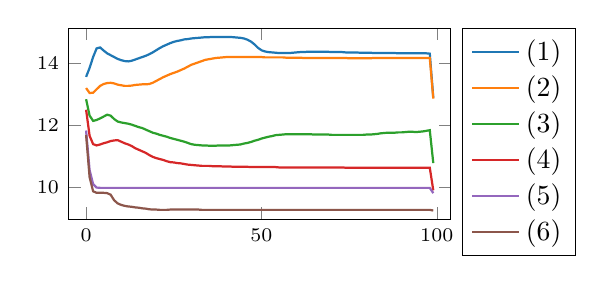
\begin{tikzpicture}

\definecolor{crimson2143940}{RGB}{214,39,40}
\definecolor{darkgray176}{RGB}{176,176,176}
\definecolor{darkorange25512714}{RGB}{255,127,14}
\definecolor{forestgreen4416044}{RGB}{44,160,44}
\definecolor{mediumpurple148103189}{RGB}{148,103,189}
\definecolor{sienna1408675}{RGB}{140,86,75}
\definecolor{steelblue31119180}{RGB}{31,119,180}

\begin{axis}[compar, legend pos=outer north east]
\addplot [thick, steelblue31119180]
table {%
0 13.5699996948242
1 13.8599996566772
2 14.210000038147
3 14.4899997711182
4 14.5200004577637
5 14.4200000762939
6 14.3299999237061
9 14.1499996185303
10 14.1099996566772
11 14.0799999237061
12 14.0699996948242
13 14.0900001525879
17 14.25
18 14.3000001907349
19 14.3599996566772
21 14.5
22 14.5600004196167
24 14.6599998474121
25 14.6999998092651
26 14.7299995422363
27 14.75
28 14.7799997329712
29 14.789999961853
30 14.8100004196167
34 14.8500003814697
35 14.8500003814697
36 14.8599996566772
41 14.8599996566772
44 14.8299999237061
45 14.8100004196167
46 14.7700004577637
47 14.710000038147
48 14.6199998855591
49 14.5100002288818
50 14.4300003051758
51 14.3900003433228
52 14.3699998855591
55 14.3400001525879
58 14.3400001525879
61 14.3699998855591
62 14.3699998855591
63 14.3800001144409
69 14.3800001144409
70 14.3699998855591
73 14.3699998855591
74 14.3599996566772
77 14.3599996566772
78 14.3500003814697
81 14.3500003814697
82 14.3400001525879
88 14.3400001525879
89 14.3299999237061
97 14.3299999237061
98 14.3199996948242
99 12.8999996185303
};
\addlegendentry{$(1)$}
\addplot [thick, darkorange25512714]
table {%
0 13.210000038147
1 13.0500001907349
2 13.0600004196167
4 13.2799997329712
5 13.3400001525879
6 13.3699998855591
7 13.3800001144409
8 13.3599996566772
9 13.3199996948242
11 13.2799997329712
12 13.2799997329712
13 13.289999961853
14 13.3100004196167
16 13.3299999237061
17 13.3299999237061
18 13.3400001525879
19 13.3800001144409
22 13.5600004196167
24 13.6599998474121
26 13.7399997711182
28 13.8400001525879
30 13.960000038147
34 14.1199998855591
37 14.1800003051758
40 14.210000038147
50 14.210000038147
51 14.1999998092651
56 14.1999998092651
57 14.1899995803833
61 14.1899995803833
62 14.1800003051758
74 14.1800003051758
75 14.1700000762939
81 14.1700000762939
82 14.1800003051758
98 14.1800003051758
99 12.8699998855591
};
\addlegendentry{$(2)$}
\addplot [thick, forestgreen4416044]
table {%
0 12.8500003814697
1 12.3199996948242
2 12.1499996185303
3 12.1800003051758
4 12.2299995422363
6 12.3500003814697
7 12.3199996948242
8 12.210000038147
9 12.1300001144409
10 12.1000003814697
12 12.0600004196167
13 12.0299997329712
15 11.9499998092651
16 11.9200000762939
19 11.7700004577637
20 11.7399997711182
21 11.6999998092651
23 11.6400003433228
24 11.6000003814697
28 11.4799995422363
30 11.3999996185303
31 11.3800001144409
33 11.3599996566772
34 11.3599996566772
35 11.3500003814697
37 11.3500003814697
38 11.3599996566772
41 11.3599996566772
44 11.3900003433228
45 11.4200000762939
46 11.4399995803833
47 11.4700002670288
48 11.5100002288818
49 11.539999961853
50 11.5799999237061
52 11.6400003433228
53 11.6599998474121
54 11.6899995803833
57 11.7200002670288
64 11.7200002670288
65 11.710000038147
69 11.710000038147
70 11.6999998092651
79 11.6999998092651
80 11.710000038147
81 11.710000038147
83 11.7299995422363
84 11.75
86 11.7700004577637
88 11.7700004577637
89 11.7799997329712
90 11.7799997329712
92 11.8000001907349
93 11.8000001907349
94 11.789999961853
96 11.8100004196167
98 11.8500003814697
99 10.789999961853
};
\addlegendentry{$(3)$}
\addplot [thick, crimson2143940]
table {%
0 12.5100002288818
1 11.6700000762939
2 11.3999996185303
3 11.3599996566772
4 11.3900003433228
5 11.4300003051758
6 11.460000038147
7 11.5
8 11.5200004577637
9 11.5299997329712
11 11.4300003051758
12 11.3900003433228
13 11.3400001525879
14 11.2700004577637
17 11.1199998855591
18 11.0500001907349
19 10.9899997711182
20 10.9499998092651
22 10.8900003433228
23 10.8500003814697
24 10.8199996948242
25 10.8100004196167
26 10.789999961853
27 10.7799997329712
29 10.7399997711182
33 10.6999998092651
35 10.6999998092651
36 10.6899995803833
38 10.6899995803833
39 10.6800003051758
41 10.6800003051758
42 10.6700000762939
46 10.6700000762939
47 10.6599998474121
54 10.6599998474121
55 10.6499996185303
73 10.6499996185303
74 10.6400003433228
98 10.6400003433228
99 9.90999984741211
};
\addlegendentry{$(4)$}
\addplot [thick, mediumpurple148103189]
table {%
0 11.8400001525879
1 10.5600004196167
2 10.1099996566772
3 10
4 9.98999977111816
98 9.98999977111816
99 9.81999969482422
};
\addlegendentry{$(5)$}
\addplot [thick, sienna1408675]
table {%
0 11.6999998092651
1 10.3299999237061
2 9.88000011444092
3 9.82999992370605
5 9.82999992370605
6 9.81999969482422
7 9.77000045776367
8 9.59000015258789
9 9.48999977111816
10 9.4399995803833
11 9.40999984741211
12 9.39000034332275
13 9.38000011444092
14 9.35999965667725
15 9.35000038146973
16 9.32999992370605
17 9.31999969482422
18 9.30000019073486
19 9.28999996185303
20 9.28999996185303
21 9.27999973297119
23 9.27999973297119
24 9.28999996185303
32 9.28999996185303
33 9.27999973297119
98 9.27999973297119
99 9.26000022888184
};
\addlegendentry{$(6)$}
\end{axis}

\end{tikzpicture}
}
\end{tabular}
    \caption{Comparaison de la PGD avec le résultat attendu (Target) après 100 itérations et avec différent pas --- initialisation $^tA(Ax)$, passe-bas gaussien ($\sigma=0.6$)}
\end{figure}




\newpage



\section{Conclusion}

Par manque de temps, il n'a pas été trop possible de trop rentrer dans la théorie mais au vue des résultats il est clair que qu'il y a quelque chose à voir.  
\\
Il a été fait le choix de de supposer $f_D$ inversible pour exprimer le fait que $f_D$ vienne qu'un auto-encodeur. Mais peut-être qu'une formalisation moins dur, pas exemple en terme de voisinage, de cette idée pourrait être moins restrictive. En particulier, avoir $\ d\big(\theta, \theta^*\big)=\big\|\theta-\theta^*\big\|_2\ $ plutôt qu'une égalité permettrait d'élargir le bassin $\Lambda_\beta$, ce qui serait plus cohérent avec les résultats
\\

A voir sur des images plus complexes mais \apriori, les modèles très résistant à l'aliasing
\\

Il faudrait faire marcher le pas adaptatif voir ajouter de l'inertie pour éviter les cas les plateaux qui arrive de temps à autre.




\newpage





\begin{annexe}
\section{Annexes}

\subsection{Auto-encodeur}\label{anx:AE}
\quad

Comme expliqué en début de rapport, section \ref{sec:forma2pb}, les auto-encodeurs utilisés, sont des réseaux MLP comptant une couche cachée de taille 1500 pour les parties encodage et décodage, et d'espace latent de taille respective 100, 200, 400 et 800. Pour reprendre ce qui a été fait par Peng \etal, tout les fonctions d'activations sont des sigmoïdes, ce qui, retrospectivement, n'était pas le plus judicieux (\cf section \ref{sec:article1/2}).
\\
Leur entraînement s'est fait sur le jeu de données MNIST sur 60 epochs avec des batchs de tailles 100.  Il est effectué par le code \texttt{training autoencoder.py} disponible sur le  \href{https://www.youtube.com/watch?v=dQw4w9WgXcQ&pp=ygUIcmlja3JvbGw%3D}{GitHub} et dont voici un résumé des performances :
\\
\begin{figure}[H]\centering
    \setlength{\tabcolsep}{3pt}
\begin{tabular}{ c c c c c c c c c }

\rotatebox[origin=lt]{90}{Input}
&
\includegraphics[width=0.11\textwidth]{resultats/auto-encoder/AE-100_1_input.png}
&
\includegraphics[width=0.11\textwidth]{resultats/auto-encoder/AE-100_2_input.png}
&
\includegraphics[width=0.11\textwidth]{resultats/auto-encoder/AE-100_3_input.png}
&
\includegraphics[width=0.11\textwidth]{resultats/auto-encoder/AE-100_4_input.png}
&
\includegraphics[width=0.11\textwidth]{resultats/auto-encoder/AE-100_5_input.png}
&
\includegraphics[width=0.11\textwidth]{resultats/auto-encoder/AE-100_6_input.png}
&
\includegraphics[width=0.11\textwidth]{resultats/auto-encoder/AE-100_7_input.png}
&
\includegraphics[width=0.11\textwidth]{resultats/auto-encoder/AE-100_8_input.png}

\\ %\hline

\rotatebox[origin=lt]{90}{\quad\ }
&
{\scriptsize PSNR=24.63}
&
{\scriptsize PSNR=28.57}
&
{\scriptsize PSNR=26.74}
&
{\scriptsize PSNR=25.1}
&
{\scriptsize PSNR=25.86}
&
{\scriptsize PSNR=25.3867}
&
{\scriptsize PSNR=27.96}
&
{\scriptsize PSNR=28.21}

\\

\rotatebox[origin=lt]{90}{\ \ 100}
&
\includegraphics[width=0.11\textwidth]{resultats/auto-encoder/AE-100_1_PSNR=24.63_output.png}
&
\includegraphics[width=0.11\textwidth]{resultats/auto-encoder/AE-100_2_PSNR=28.57_output.png}
&
\includegraphics[width=0.11\textwidth]{resultats/auto-encoder/AE-100_3_PSNR=26.74_output.png}
&
\includegraphics[width=0.11\textwidth]{resultats/auto-encoder/AE-100_4_PSNR=25.1_output.png}
&
\includegraphics[width=0.11\textwidth]{resultats/auto-encoder/AE-100_5_PSNR=25.86_output.png}
&
\includegraphics[width=0.11\textwidth]{resultats/auto-encoder/AE-100_6_PSNR=29.67_output.png}
&
\includegraphics[width=0.11\textwidth]{resultats/auto-encoder/AE-100_7_PSNR=27.96_output.png}
&
\includegraphics[width=0.11\textwidth]{resultats/auto-encoder/AE-100_8_PSNR=28.21_output.png}

\\

\rotatebox[origin=lt]{90}{\quad\ }
&
{\scriptsize PSNR=25.38}
&
{\scriptsize PSNR=29.88}
&
{\scriptsize PSNR=28.31}
&
{\scriptsize PSNR=25.17}
&
{\scriptsize PSNR=27.27}
&
{\scriptsize PSNR=31.16}
&
{\scriptsize PSNR=28.34}
&
{\scriptsize PSNR=28.1}

\\

\rotatebox[origin=lt]{90}{\ \ 200}
&
\includegraphics[width=0.11\textwidth]{resultats/auto-encoder/AE-200_1_PSNR=25.38_output.png}
&
\includegraphics[width=0.11\textwidth]{resultats/auto-encoder/AE-200_2_PSNR=29.88_output.png}
&
\includegraphics[width=0.11\textwidth]{resultats/auto-encoder/AE-200_3_PSNR=28.31_output.png}
&
\includegraphics[width=0.11\textwidth]{resultats/auto-encoder/AE-200_4_PSNR=25.17_output.png}
&
\includegraphics[width=0.11\textwidth]{resultats/auto-encoder/AE-200_5_PSNR=27.27_output.png}
&
\includegraphics[width=0.11\textwidth]{resultats/auto-encoder/AE-200_6_PSNR=31.16_output.png}
&
\includegraphics[width=0.11\textwidth]{resultats/auto-encoder/AE-200_7_PSNR=28.34_output.png}
&
\includegraphics[width=0.11\textwidth]{resultats/auto-encoder/AE-200_8_PSNR=28.1_output.png}

\\

\rotatebox[origin=lt]{90}{\quad\ }
&
{\scriptsize PSNR=26.15}
&
{\scriptsize PSNR=31.25}
&
{\scriptsize PSNR=28.97}
&
{\scriptsize PSNR=26.13}
&
{\scriptsize PSNR=27.76}
&
{\scriptsize PSNR=31.64}
&
{\scriptsize PSNR=29.69}
&
{\scriptsize PSNR=29.75}

\\

\rotatebox[origin=lt]{90}{\ \ 400}
&
\includegraphics[width=0.11\textwidth]{resultats/auto-encoder/AE-400_1_PSNR=26.15_output.png}
&
\includegraphics[width=0.11\textwidth]{resultats/auto-encoder/AE-400_2_PSNR=31.25_output.png}
&
\includegraphics[width=0.11\textwidth]{resultats/auto-encoder/AE-400_3_PSNR=28.97_output.png}
&
\includegraphics[width=0.11\textwidth]{resultats/auto-encoder/AE-400_4_PSNR=26.13_output.png}
&
\includegraphics[width=0.11\textwidth]{resultats/auto-encoder/AE-400_5_PSNR=27.76_output.png}
&
\includegraphics[width=0.11\textwidth]{resultats/auto-encoder/AE-400_6_PSNR=31.64_output.png}
&
\includegraphics[width=0.11\textwidth]{resultats/auto-encoder/AE-400_7_PSNR=29.69_output.png}
&
\includegraphics[width=0.11\textwidth]{resultats/auto-encoder/AE-400_8_PSNR=29.75_output.png}

\\

\rotatebox[origin=lt]{90}{\quad\ }
&
{\scriptsize PSNR=27.55}
&
{\scriptsize PSNR=31.21}
&
{\scriptsize PSNR=30.24}
&
{\scriptsize PSNR=27.6}
&
{\scriptsize PSNR=29.67}
&
{\scriptsize PSNR=32.97}
&
{\scriptsize PSNR=29.73}
&
{\scriptsize PSNR=30.72}

\\

\rotatebox[origin=lt]{90}{\ \ 800}
&
\includegraphics[width=0.11\textwidth]{resultats/auto-encoder/AE-800_1_PSNR=27.55_output.png}
&
\includegraphics[width=0.11\textwidth]{resultats/auto-encoder/AE-800_2_PSNR=31.21_output.png}
&
\includegraphics[width=0.11\textwidth]{resultats/auto-encoder/AE-800_3_PSNR=30.24_output.png}
&
\includegraphics[width=0.11\textwidth]{resultats/auto-encoder/AE-800_4_PSNR=27.6_output.png}
&
\includegraphics[width=0.11\textwidth]{resultats/auto-encoder/AE-800_5_PSNR=29.67_output.png}
&
\includegraphics[width=0.11\textwidth]{resultats/auto-encoder/AE-800_6_PSNR=32.97_output.png}
&
\includegraphics[width=0.11\textwidth]{resultats/auto-encoder/AE-800_7_PSNR=29.73_output.png}
&
\includegraphics[width=0.11\textwidth]{resultats/auto-encoder/AE-800_8_PSNR=30.72_output.png}

\end{tabular}
    \caption{Reconstruction par auto-encodeur des images Input en fonction de la taille de l'espace latent du dit auto-encodeur et avec les PSNR associés}
    \label{fig:AEapp}
\end{figure}
\begin{figure}[H]\centering
    \setlength{\tabcolsep}{0pt}
\begin{tabular}{r r r r r}

& &  Autoencoder 100{\color{white}bbbb}  &  Autoencoder 200{\color{white}bbbb}  &  Autoencoder 400{\color{white}bbbb}  

\\ \\

\rotatebox[origin=lt]{90}{{\color{white}bbbb}MSE}
& &
% This file was created with tikzplotlib v0.10.1.
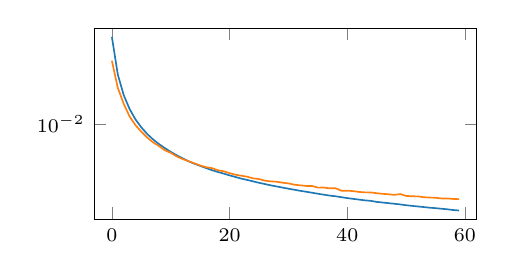
\begin{tikzpicture}

\definecolor{darkgray176}{RGB}{176,176,176}
\definecolor{darkorange25512714}{RGB}{255,127,14}
\definecolor{steelblue31119180}{RGB}{31,119,180}

\begin{axis}[compar,
ymode=log]
\addplot [semithick, steelblue31119180]
table {%
0 0.0518720038235188
1 0.02554801851511
2 0.0173378624022007
3 0.0133188515901566
4 0.0109316576272249
5 0.00939567107707262
6 0.00828651990741491
7 0.00748166767880321
8 0.00685237208381295
9 0.00635064486414194
10 0.00591443525627255
11 0.00555017963051796
12 0.00523966317996383
13 0.00495978863909841
14 0.00473269680514932
15 0.00453824829310179
17 0.00418460322543979
18 0.00404801033437252
19 0.00392276374623179
20 0.00379281048662961
21 0.00368099054321647
22 0.00356699386611581
23 0.00348103558644652
25 0.00329699576832354
26 0.00322135980241001
27 0.00314237107522786
29 0.00301361549645662
30 0.00294889183714986
31 0.00289292447268963
32 0.00283385463990271
33 0.00278664077632129
35 0.00268257665447891
37 0.00258983112871647
38 0.00255701458081603
40 0.00246976083144546
43 0.00236683199182153
44 0.00234519876539707
45 0.00229926710017025
48 0.00221881736069918
49 0.00219219038262963
50 0.00215819384902716
54 0.00206096656620502
55 0.00204216712154448
57 0.00199954304844141
58 0.0019717204850167
59 0.00195437553338706
};
\addplot [semithick, darkorange25512714]
table {%
0 0.0330518148839474
1 0.0198523905128241
2 0.0147118531167507
3 0.0115565303713083
4 0.00981095712631941
5 0.00865060556679964
6 0.00774995889514685
7 0.00707322917878628
8 0.00661052903160453
9 0.00609223870560527
10 0.00581139419227839
11 0.00543221551924944
12 0.00516849244013429
13 0.00497076008468866
15 0.00457627838477492
16 0.0044299834407866
17 0.00435137096792459
18 0.00418223068118095
19 0.00410104729235172
20 0.00395805621519685
21 0.00384121690876782
23 0.00369861349463463
24 0.00358767551369965
25 0.00353957526385784
26 0.00343360542319715
27 0.00338863302022219
28 0.00336424726992846
29 0.00330294319428504
30 0.00326295848935843
31 0.00318127800710499
33 0.00310822506435215
34 0.00310828490182757
35 0.0030126660130918
36 0.00301306950859725
37 0.00297222589142621
38 0.00297658750787377
39 0.00283884350210428
40 0.00284207612276077
41 0.00281827640719712
42 0.00277460599318147
43 0.00275322678498924
44 0.00274799601174891
45 0.00271018617786467
46 0.00267772865481675
47 0.00265605910681188
48 0.00262555666267872
49 0.0026655406691134
50 0.00257417652755976
51 0.00255639688111842
52 0.00255104713141918
53 0.00251109828241169
54 0.0024961472954601
55 0.00248667155392468
56 0.00245288014411926
57 0.0024546233471483
58 0.00243026949465275
59 0.0024220822378993
};
\end{axis}

\end{tikzpicture}

&
% This file was created with tikzplotlib v0.10.1.
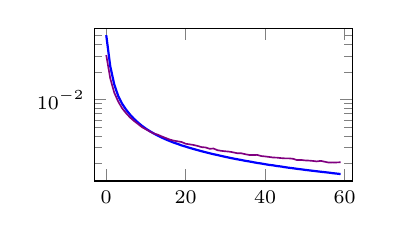
\begin{tikzpicture}

\definecolor{darkgray176}{RGB}{176,176,176}
\definecolor{darkorange25512714}{RGB}{255,127,14}
\definecolor{steelblue31119180}{RGB}{31,119,180}

\begin{axis}[speAE,
ymode=log,
ytick={0.0001,0.001,0.01,0.1,1},
yticklabels={
  \(\displaystyle {10^{-4}}\),
  \(\displaystyle {10^{-3}}\),
  \(\displaystyle {10^{-2}}\),
  \(\displaystyle {10^{-1}}\),
  \(\displaystyle {10^{0}}\)
}
]
\addplot [thick, blue]
table {%
0 0.0503827184438705
1 0.0231762751936913
2 0.014697564765811
3 0.0109478253871202
4 0.00899229943752289
5 0.00774224475026131
6 0.00684232404455543
7 0.00614844681695104
8 0.00560816191136837
9 0.00516596203669906
10 0.00480720214545727
11 0.00450789043679833
12 0.00425539258867502
13 0.00403159903362393
14 0.00384168932214379
15 0.00366993132047355
16 0.00352168921381235
17 0.00338485115207732
18 0.00327525730244815
19 0.00315655907616019
20 0.00306433159857988
21 0.00296860747039318
23 0.00280534545890987
24 0.00272952229715884
26 0.0025950912386179
27 0.00253195920959115
28 0.00247928220778704
29 0.00242134579457343
31 0.00231824209913611
33 0.00222833012230694
34 0.00218915846198797
35 0.00214463635347784
36 0.00211104960180819
38 0.00203325902111828
39 0.00200548488646746
40 0.00196877960115671
41 0.00193660240620375
42 0.00191451469436288
43 0.00188098242506385
44 0.00185941788367927
45 0.00182812963612378
46 0.00180087820626795
47 0.0017799154156819
48 0.00175378890708089
49 0.001733677694574
50 0.00170948228333145
54 0.00162926164921373
56 0.00159461738076061
57 0.00157220743130893
58 0.00155619683209807
59 0.00153788621537387
};
\addplot [semithick, violet]
table {%
0 0.0305683203041553
1 0.017071396112442
2 0.011926488019526
3 0.00952861737459898
4 0.0080207260325551
5 0.00709329778328538
6 0.00636689830571413
7 0.0058362390846014
8 0.00540540693327785
9 0.00499403430148959
11 0.0044674351811409
12 0.00425342144444585
13 0.00413477141410112
14 0.00395425315946341
16 0.00365695520304143
17 0.00355988088995218
18 0.0035015782341361
19 0.00343526271171868
20 0.0032912774477154
21 0.00324278487823904
22 0.00319049344398081
23 0.00311692943796515
24 0.00302586634643376
25 0.00299932225607336
26 0.00290136504918337
27 0.00292090233415365
28 0.00279996660538018
29 0.00275404471904039
30 0.00272374297492206
31 0.0027005102019757
32 0.00265146419405937
33 0.00259227468632162
34 0.00259035988710821
35 0.00253120018169284
36 0.00248397560790181
37 0.00248199491761625
38 0.0024878759868443
39 0.00241875112988055
40 0.00239369249902666
41 0.00236381567083299
42 0.00233046384528279
43 0.00232217158190906
44 0.00229623098857701
45 0.00228002434596419
46 0.00228015333414078
47 0.0022583685349673
48 0.00218693865463138
49 0.00219371449202299
50 0.00216764211654663
51 0.00215686019510031
52 0.00213886913843453
53 0.0021116673015058
54 0.00214252411387861
56 0.00205086614005268
57 0.00205984897911549
58 0.00205883500166237
59 0.00206905510276556
};
\end{axis}

\end{tikzpicture}

&
% This file was created with tikzplotlib v0.10.1.
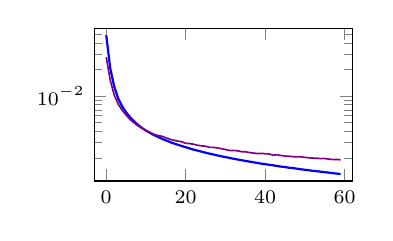
\begin{tikzpicture}

\definecolor{darkgray176}{RGB}{176,176,176}
\definecolor{darkorange25512714}{RGB}{255,127,14}
\definecolor{steelblue31119180}{RGB}{31,119,180}

\begin{axis}[speAE,
ymode=log,
ytick={0.0001,0.001,0.01,0.1,1},
yticklabels={
  \(\displaystyle {10^{-4}}\),
  \(\displaystyle {10^{-3}}\),
  \(\displaystyle {10^{-2}}\),
  \(\displaystyle {10^{-1}}\),
  \(\displaystyle {10^{0}}\)
}
]
\addplot [thick, blue]
table {%
0 0.0492035262286663
1 0.0207414887845516
2 0.0129387434571981
3 0.00945419538766146
4 0.00766767701134086
5 0.00656204577535391
6 0.00578529853373766
7 0.00518497824668884
8 0.00472294026985765
9 0.00436683231964707
10 0.00407265918329358
12 0.00362355192191899
14 0.00329436152242124
16 0.00302357808686793
18 0.0028144761454314
20 0.00263713044114411
22 0.00247619464062154
23 0.0024149629753083
25 0.00228715874254704
28 0.00212763133458793
30 0.00204079411923885
32 0.00195532198995352
35 0.00184639461804181
36 0.00181616784539074
37 0.00178282673005015
38 0.00175259064417332
39 0.00171963183674961
41 0.00166981155052781
42 0.00164510158356279
44 0.00159098510630429
45 0.00157107796985656
46 0.00154567917343229
47 0.00153023435268551
49 0.00148346740752459
50 0.00146513234358281
52 0.00142524391412735
53 0.00141107453964651
55 0.00137436343356967
56 0.00136018230114132
57 0.00134005874861032
58 0.00132755958475173
59 0.00130976806394756
};
\addplot [semithick, violet]
table {%
0 0.0276999436318874
1 0.0152005106210709
2 0.0103711616247892
3 0.00814399775117636
4 0.00693845562636852
5 0.00611581327393651
6 0.00544816395267844
7 0.00498418230563402
8 0.00461689289659262
9 0.00433709705248475
10 0.0040805097669363
11 0.00389086711220443
12 0.00370007567107677
13 0.00358308735303581
14 0.00351104489527643
15 0.00338523765094578
16 0.00325000286102295
17 0.00316429394297302
18 0.00309449038468301
19 0.00304547790437937
20 0.00292374682612717
21 0.00290122651495039
22 0.00285399938002229
23 0.00277612800709903
24 0.00273615051992238
25 0.00271024717949331
26 0.00262898951768875
27 0.0026314384303987
28 0.00259054196067154
29 0.00254159467294812
30 0.00248572020791471
31 0.00242716423235834
32 0.00242336583323777
33 0.00240683532319963
34 0.0023516824003309
35 0.00234355125576258
36 0.00229976209811866
37 0.00226869224570692
38 0.00223404658026993
39 0.00224652979522943
40 0.00222630659118295
41 0.00221177469938993
42 0.00214156811125576
43 0.00216725165955722
44 0.00212531164288521
45 0.00209872331470251
46 0.0020835162140429
47 0.00206287042237818
48 0.0020514854695648
49 0.00205233367159963
50 0.00202494696713984
51 0.00200132979080081
52 0.00198752526193857
53 0.00198013707995415
54 0.00196109595708549
55 0.00196250132285058
57 0.00191261433064938
58 0.00191620655823499
59 0.00189937290269881
};
\end{axis}

\end{tikzpicture}


\\

\rotatebox[origin=lt]{90}{{\color{white}bbbb}PSNR}
& &
% This file was created with tikzplotlib v0.10.1.
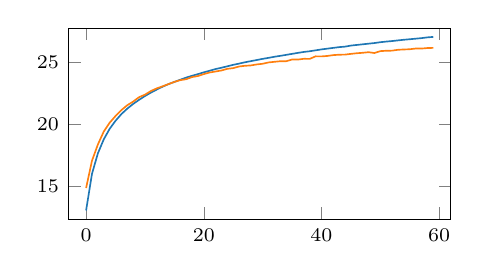
\begin{tikzpicture}

\definecolor{darkgray176}{RGB}{176,176,176}
\definecolor{darkorange25512714}{RGB}{255,127,14}
\definecolor{steelblue31119180}{RGB}{31,119,180}

\begin{axis}[compar]
\addplot [semithick, steelblue31119180]
table {%
0 12.9921646118164
1 15.9709796905518
2 17.6316299438477
3 18.7714214324951
4 19.6243877410889
5 20.2814331054688
6 20.825569152832
7 21.2693367004395
8 21.6509838104248
9 21.9818019866943
10 22.290246963501
11 22.5658435821533
12 22.8153610229492
13 23.0541896820068
14 23.2580280303955
15 23.4398918151855
17 23.7910099029541
18 23.9354858398438
19 24.0712852478027
20 24.2189025878906
21 24.3479061126709
22 24.4848308563232
23 24.5913696289062
25 24.826379776001
26 24.9274959564209
27 25.0352840423584
29 25.2175579071045
30 25.3115119934082
31 25.3935966491699
32 25.4829597473145
33 25.556453704834
36 25.7987403869629
37 25.8744373321533
38 25.9299793243408
40 26.0803718566895
43 26.2660179138184
44 26.3055362701416
45 26.3908996582031
48 26.5458984375
49 26.5972957611084
50 26.6657619476318
51 26.715425491333
52 26.7595901489258
54 26.8653030395508
55 26.9054412841797
57 26.9971542358398
58 27.0580635070801
59 27.0958271026611
};
\addplot [semithick, darkorange25512714]
table {%
0 14.8166589736938
1 17.0394096374512
2 18.3499698638916
3 19.4052104949951
4 20.12087059021
5 20.6666812896729
6 21.1473579406738
7 21.5459537506104
8 21.8410625457764
9 22.1983013153076
10 22.4017715454102
11 22.6959228515625
12 22.9133548736572
13 23.081262588501
15 23.4413452148438
16 23.5824241638184
17 23.658863067627
18 23.8318309783936
19 23.9167766571045
20 24.0732536315918
21 24.2038154602051
23 24.3677520751953
24 24.5024852752686
25 24.5585422515869
26 24.6924247741699
27 24.7486114501953
28 24.7782421112061
29 24.8595581054688
30 24.9125595092773
31 25.0220222473145
33 25.1214275360107
34 25.1195774078369
35 25.2583465576172
36 25.2555713653564
37 25.3172721862793
38 25.3094215393066
39 25.5182762145996
40 25.5110721588135
41 25.5484962463379
42 25.6167793273926
43 25.6492214202881
44 25.6571216583252
45 25.7165641784668
46 25.7686500549316
47 25.8048152923584
48 25.8545074462891
49 25.786994934082
50 25.9404563903809
51 25.9712791442871
52 25.9788265228271
53 26.0497512817383
54 26.0743026733398
55 26.0925235748291
56 26.1517753601074
57 26.1480541229248
58 26.1905174255371
59 26.2049503326416
};
\end{axis}

\end{tikzpicture}

&
% This file was created with tikzplotlib v0.10.1.
\begin{tikzpicture}

\definecolor{darkgray176}{RGB}{176,176,176}
\definecolor{darkorange25512714}{RGB}{255,127,14}
\definecolor{steelblue31119180}{RGB}{31,119,180}

\begin{axis}[
height=\figheight,
tick align=outside,
tick pos=left,
width=\figwidth,
x grid style={darkgray176},
xmin=-2.95, xmax=61.95,
xtick style={color=black},
y grid style={darkgray176},
ymin=12.3918090820312, ymax=28.8864463806152,
ytick style={color=black}
]
\addplot [semithick, steelblue31119180]
table {%
0 13.141565322876
1 16.4121437072754
2 18.3559398651123
3 19.6229076385498
4 20.4739570617676
5 21.121940612793
6 21.6586933135986
7 22.1230201721191
8 22.5214576721191
9 22.8782615661621
10 23.190357208252
11 23.4693088531494
12 23.7187671661377
13 23.9537391662598
14 24.1627216339111
15 24.3614559173584
17 24.7117385864258
18 24.8552265167236
19 25.0149211883545
20 25.1446475982666
21 25.2817459106445
23 25.5281562805176
24 25.6464061737061
26 25.8652076721191
27 25.9728870391846
28 26.0626010894775
29 26.1668891906738
31 26.3553466796875
33 26.5267696380615
34 26.6037197113037
35 26.6926212310791
36 26.7621040344238
38 26.9245300292969
39 26.9842643737793
40 27.0646324157715
41 27.1359672546387
42 27.1858768463135
43 27.2623500823975
44 27.3123149871826
45 27.3857326507568
46 27.4515209197998
47 27.502025604248
48 27.5662307739258
49 27.6161918640137
50 27.6774291992188
54 27.8856678009033
56 27.9792156219482
57 28.0409603118896
58 28.0852375030518
59 28.1366901397705
};
\addplot [semithick, darkorange25512714]
table {%
0 15.1579599380493
1 17.7009410858154
2 19.2677421569824
3 20.2477607727051
4 21.000602722168
5 21.5357780456543
6 22.0056056976318
7 22.3844528198242
8 22.7170639038086
9 23.0631332397461
11 23.5465240478516
12 23.761116027832
13 23.8813629150391
14 24.0759983062744
16 24.4174518585205
17 24.5327701568604
18 24.6020584106445
19 24.686107635498
20 24.8729763031006
22 25.0086402893066
23 25.1091575622559
24 25.2393856048584
25 25.2758560180664
26 25.4226875305176
27 25.3897819519043
28 25.5762500762939
29 25.6475467681885
30 25.6960620880127
31 25.7340679168701
32 25.8129272460938
33 25.9113426208496
34 25.9128532409668
35 26.0150375366211
36 26.0973606109619
37 26.0996189117432
38 26.0877342224121
39 26.2120475769043
40 26.2576656341553
41 26.3121719360352
42 26.3743019104004
43 26.388822555542
44 26.4381885528564
45 26.4681549072266
46 26.4669132232666
47 26.5092792510986
48 26.650764465332
49 26.6363906860352
50 26.6879081726074
51 26.709623336792
52 26.7456436157227
53 26.8024978637695
54 26.7362613677979
55 26.830005645752
56 26.9311370849609
57 26.9100170135498
58 26.911470413208
59 26.8904571533203
};
\end{axis}

\end{tikzpicture}

&
% This file was created with tikzplotlib v0.10.1.
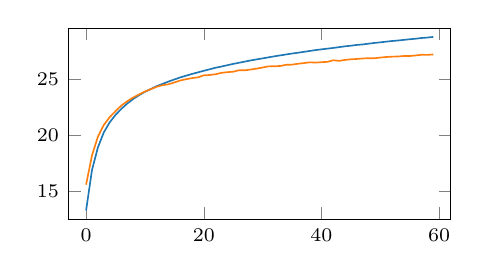
\begin{tikzpicture}

\definecolor{darkgray176}{RGB}{176,176,176}
\definecolor{darkorange25512714}{RGB}{255,127,14}
\definecolor{steelblue31119180}{RGB}{31,119,180}

\begin{axis}[compar]
\addplot [semithick, steelblue31119180]
table {%
0 13.2728042602539
1 16.8960628509521
2 18.9158535003662
3 20.2616062164307
4 21.1672916412354
5 21.8417053222656
6 22.3864879608154
7 22.8624649047852
8 23.2667961120605
9 23.6068515777588
10 23.9097938537598
12 24.4168853759766
14 24.8300304412842
16 25.2024040222168
18 25.5130214691162
20 25.7950820922852
22 26.0686435699463
23 26.1776180267334
25 26.4130954742432
28 26.7272052764893
30 26.9088249206543
32 27.0939693450928
35 27.3428802490234
36 27.413818359375
39 27.651948928833
40 27.7185516357422
42 27.8439426422119
44 27.9892120361328
45 28.0439777374268
46 28.1142082214355
47 28.157564163208
49 28.2926139831543
50 28.3467178344727
52 28.4665489196777
53 28.5100154876709
55 28.6242618560791
56 28.6696815490723
57 28.73388671875
58 28.7748146057129
59 28.8332748413086
};
\addplot [semithick, darkorange25512714]
table {%
0 15.5871000289917
1 18.2080001831055
2 19.8783931732178
3 20.9324569702148
4 21.6307258605957
5 22.1794261932373
6 22.6829452514648
7 23.0694847106934
8 23.4025821685791
10 23.9384956359863
11 24.1459331512451
12 24.3642425537109
13 24.5037326812744
14 24.5904636383057
15 24.7491874694824
16 24.9271564483643
17 25.0406379699707
18 25.1383953094482
19 25.2085819244385
20 25.3868732452393
21 25.417516708374
22 25.4887542724609
23 25.6104412078857
24 25.6722221374512
25 25.7123947143555
26 25.8468799591064
27 25.840425491333
28 25.910120010376
29 25.9917697906494
30 26.0894184112549
31 26.1942081451416
32 26.1996917724609
33 26.2298202514648
34 26.3323268890381
35 26.3461246490479
36 26.4279403686523
37 26.4865188598633
38 26.5542278289795
39 26.528959274292
40 26.5687160491943
41 26.5965518951416
42 26.738151550293
43 26.6855964660645
44 26.7709846496582
45 26.8254051208496
46 26.8574275970459
47 26.9000606536865
48 26.9245586395264
49 26.922248840332
50 26.9806575775146
51 27.0315456390381
52 27.0615119934082
53 27.0784149169922
54 27.1207332611084
55 27.1165866851807
57 27.2284736633301
58 27.2209587097168
59 27.2595596313477
};
\end{axis}

\end{tikzpicture}

\end{tabular}
    \caption{Évolution de la MSE et du PSNR par batch des auto-encodeurs au cours des epochs. En bleu sur le set d'entraînement et en violet sur celui de test}
    \label{fig:AEperf}
\end{figure}
%\\ \\



\subsection{Calcul pratique de $\bf{F}$ et de son gradient}\label{anx:gradF}
\quad

\begin{enonce}[Notation]
Comme $A$ est linéaire, dans toute la suite elle sera assimilé à matrice la représentant. Là où l'opérateur $A$ prend pour entrée un image $\bf{x}\in\R^{n\times m}$, sa représentation matricielle elle prendre un vecteur $x\in\R^{nm}$. Par souci de lisibilité on notera dans toute la suite les images sous forme de matrice en gras, leur version vectorielle en fin.
\end{enonce}

Le fait de supposer $A$ linéaire permet de calcul explicitement le gradient de $F$ à moindre coût :
\begin{equation}\label{eq:gradient}
\forall x\in\R^{nm},\qquad \nabla F(x)=\,^tA\big(Ax-y\big)
\end{equation}{\color{white}l}
Si la formule (\ref{eq:gradient}) est mathématiquement très simple, dès que $n$ et $m$ seront un peu trop grand, la taille de $A$ va très vite ralentir tout algorithme de descente et prendre énormément de place en mémoire.

Pour éviter d'avoir à construire à explicitement on passe par la transformée de Fourier. On note $\F$ (resp. $\F^{-1}$) la matrice associée à la transformée (resp. inverse) de Fourier discrète. En notant de plus $\hat{\bf{x}}=\F \bf{x}$ et $\odot$ le produit terme à terme de vecteur/matrice, $A$ s'écrit alors :
\begin{align*}\forall \bf{x}\in\R^{n\times m},\qquad A(\bf{x})=S\circ C_h(\bf{x})=S(\bf{h}*\bf{x})&=S\circ\F^{-1}\F(\bf{h}*\bf{x})\\
    &=S\circ\F^{-1}\big(\hat{\bf{h}}\odot\hat{\bf{x}}\big)\end{align*}
\\
Notons $D_h$ l'application/matrice associée au produit $\hat{h}\odot\cdot$. Comme la transformée de Fourier discrète et $D_h$ sont symétriques\footnote{comme $x$ a été aplatie, $\F$ n'est pas diagonale à proprement parler, nous y revenons plus loin}, le gradient de $F$ se réécrire comme :
\begin{align*}\forall x\in\R^{nm},\qquad \nabla F(x)=\,^tA\big(Ax-y\big)&=\,^t\Big(S\F^{-1}D_h\F\Big)\big(S\F^{-1}D_h\F x-y\big)\\
    &=\,^t\F\,^tD_h\,^t\F^{-1}\,^tS\big(S\F^{-1}D_h\F x-y\big)\\
    &=\F D_h\F^{-1}\,^tS\big(S\F^{-1}D_h\F x-y\big)\end{align*}
\\
Sous cette forme et même s'il n'en n'a pas l'air, le gradient est bien plus simple à calculer et rapide à calculer.

D'abord, la projection $S$ est très peu coûteuse en temps de calcul puisqu'elle consiste à ne garder qu'un certain nombre de pixel de l'image. Du point de vu python, il n'y a pas besoin de construire $S$, simplement de faire l'opération :
\[\forall x\in\R^{n\times m},\qquad S(x):=\texttt{Sx = x[::n//p, ::m//q]}\]

\noindent Inversement, la transposé $^tS$ à une image $y\in\R^{p\times q}$ revient à construire une image $^tSy=$\pyt{tSy} de taille $(n,m)$ remplie de 0 puis de faire la modification :
\[\forall (i,j)\in\llbracket1,p\rrbracket\times\llbracket1,q\rrbracket,\qquad \texttt{tSy[i*n//p, j*p//q] = y[i,j]}\]{\color{white}l}

Il n'y a pas besoin non plus de construire $D_h$, le produit $\hat{\bf{h}}\odot\hat{\bf{x}}$ suffit et le passage dans/hors de l'espace des fréquences est fait pas \texttt{fft}. Ainsi, il n'y a jamais besoin d'aplatir les images et dans ce cas, on a bien la symétrie de $\F$ dans le sens où, avec les conventions ne notations d'Einstein, elle vérifie :
\[\forall(i,j)\in\llbracket1,n\rrbracket\times\llbracket1,m\rrbracket,\qquad \hat{\bf{x}}^{kl}=\F_{ ij}^{kl}\bf{x}^{ij}=\F_{ ij}^{lk}\bf{x}^{ij}=\hat{\bf{x}}^{lk}\]{\color{white}l}

Enfin, comme sont nom l'indique, il est plus naturel de construire la filtre \emph{passe-bas} directement dans l'esapce de Fourier, et ce qui est dans le code. Le figure \textit{\ref{fig:passebas-g}} et \textit{\ref{fig:passebas-p}} montre l'application de $A$ et $^tA$ à une image. La figure \textit{\ref{fig:passebas-p}} en particulier mais bien en évidence l'effet de Gibbs qui apparaît parce que les fréquences sont trop brutalement coupées.
\\
\begin{figure}[H]\centering
    \begin{tabular}{l c c c l c c c l}
$x$ & & & & $Sx$ & & & & $^tS(Sx)$
\\

\includegraphics[width=0.25\textwidth]{resultats/compare_filter/seed21-x.png}
& & & &
\includegraphics[width=0.25\textwidth]{resultats/compare_filter/seed21-Ax-filtre=s.png}
& & & &
\includegraphics[width=0.25\textwidth]{resultats/compare_filter/seed21-tA(Ax)-filtre=s.png}\end{tabular}
    \caption{Application successive de $S$ et $^tS$ à une image}
    \label{fig:sousechanti}
\end{figure}

\begin{figure}[H]\centering
    \begin{tabular}{c c c c c c}

$\sigma=0.3$  &  $\sigma=0.4$  &  $\sigma=0.5$  &  $\sigma=0.6$  &  $\sigma=0.7$ & $\sigma=0.8$

\\

\includegraphics[width=0.14\textwidth]{resultats/compare_filter/seed21-f-filtre=g_param=0.3.png}
&
\includegraphics[width=0.14\textwidth]{resultats/compare_filter/seed21-f-filtre=g_param=0.4.png}
&
\includegraphics[width=0.14\textwidth]{resultats/compare_filter/seed21-f-filtre=g_param=0.5.png}
&
\includegraphics[width=0.14\textwidth]{resultats/compare_filter/seed21-f-filtre=g_param=0.6.png}
&
\includegraphics[width=0.14\textwidth]{resultats/compare_filter/seed21-f-filtre=g_param=0.7.png}
&
\includegraphics[width=0.14\textwidth]{resultats/compare_filter/seed21-f-filtre=g_param=0.8.png}

\\ \\

\includegraphics[width=0.14\textwidth]{resultats/compare_filter/seed21-x.png}
&
\includegraphics[width=0.14\textwidth]{resultats/compare_filter/seed21-x.png}
&
\includegraphics[width=0.14\textwidth]{resultats/compare_filter/seed21-x.png}
&
\includegraphics[width=0.14\textwidth]{resultats/compare_filter/seed21-x.png}
&
\includegraphics[width=0.14\textwidth]{resultats/compare_filter/seed21-x.png}
&
\includegraphics[width=0.14\textwidth]{resultats/compare_filter/seed21-x.png}

\\ \\

\includegraphics[width=0.14\textwidth]{resultats/compare_filter/seed21-Ax-filtre=g_param=0.3.png}
&
\includegraphics[width=0.14\textwidth]{resultats/compare_filter/seed21-Ax-filtre=g_param=0.4.png}
&
\includegraphics[width=0.14\textwidth]{resultats/compare_filter/seed21-Ax-filtre=g_param=0.5.png}
&
\includegraphics[width=0.14\textwidth]{resultats/compare_filter/seed21-Ax-filtre=g_param=0.6.png}
&
\includegraphics[width=0.14\textwidth]{resultats/compare_filter/seed21-Ax-filtre=g_param=0.7.png}
&
\includegraphics[width=0.14\textwidth]{resultats/compare_filter/seed21-Ax-filtre=g_param=0.8.png}

\\ \\

\includegraphics[width=0.14\textwidth]{resultats/compare_filter/seed21-tA(Ax)-filtre=g_param=0.3.png}
&
\includegraphics[width=0.14\textwidth]{resultats/compare_filter/seed21-tA(Ax)-filtre=g_param=0.4.png}
&
\includegraphics[width=0.14\textwidth]{resultats/compare_filter/seed21-tA(Ax)-filtre=g_param=0.5.png}
&
\includegraphics[width=0.14\textwidth]{resultats/compare_filter/seed21-tA(Ax)-filtre=g_param=0.6.png}
&
\includegraphics[width=0.14\textwidth]{resultats/compare_filter/seed21-tA(Ax)-filtre=g_param=0.7.png}
&
\includegraphics[width=0.14\textwidth]{resultats/compare_filter/seed21-tA(Ax)-filtre=g_param=0.8.png}
\end{tabular}
    
    \caption{En première ligne la transformée du filtres  $\hat{\bf{h}}$ gaussien d'écart type $\sigma$, en deuxième l'image $\bf{x}$ avec en dessous le produits $A(\bf{x})$ puis $tA(A\bf{x})$.}
    \label{fig:passebas-g}
\end{figure}

\begin{figure}[H]\centering
    \begin{tabular}{c c c c c c}
$a=0.9$  &  $a=0.75$  &  $a=0.6$  &  $a=0.4$  &  $a=0.25$ & $a=0.1$

\\

\includegraphics[width=0.14\textwidth]{resultats/compare_filter/seed21-f-filtre=p_param=0.9.png}
&
\includegraphics[width=0.14\textwidth]{resultats/compare_filter/seed21-f-filtre=p_param=0.75.png}
&
\includegraphics[width=0.14\textwidth]{resultats/compare_filter/seed21-f-filtre=p_param=0.6.png}
&
\includegraphics[width=0.14\textwidth]{resultats/compare_filter/seed21-f-filtre=p_param=0.4.png}
&
\includegraphics[width=0.14\textwidth]{resultats/compare_filter/seed21-f-filtre=p_param=0.25.png}
&
\includegraphics[width=0.14\textwidth]{resultats/compare_filter/seed21-f-filtre=p_param=0.1.png}
\\



\includegraphics[width=0.14\textwidth]{resultats/compare_filter/seed21-x.png}
&
\includegraphics[width=0.14\textwidth]{resultats/compare_filter/seed21-x.png}
&
\includegraphics[width=0.14\textwidth]{resultats/compare_filter/seed21-x.png}
&
\includegraphics[width=0.14\textwidth]{resultats/compare_filter/seed21-x.png}
&
\includegraphics[width=0.14\textwidth]{resultats/compare_filter/seed21-x.png}
&
\includegraphics[width=0.14\textwidth]{resultats/compare_filter/seed21-x.png}
\\



\includegraphics[width=0.14\textwidth]{resultats/compare_filter/seed21-Ax-filtre=p_param=0.9.png}
&
\includegraphics[width=0.14\textwidth]{resultats/compare_filter/seed21-Ax-filtre=p_param=0.75.png}
&
\includegraphics[width=0.14\textwidth]{resultats/compare_filter/seed21-Ax-filtre=p_param=0.6.png}
&
\includegraphics[width=0.14\textwidth]{resultats/compare_filter/seed21-Ax-filtre=p_param=0.4.png}
&
\includegraphics[width=0.14\textwidth]{resultats/compare_filter/seed21-Ax-filtre=p_param=0.25.png}
&
\includegraphics[width=0.14\textwidth]{resultats/compare_filter/seed21-Ax-filtre=p_param=0.1.png}
\\



\includegraphics[width=0.14\textwidth]{resultats/compare_filter/seed21-tA(Ax)-filtre=p_param=0.9.png}
&
\includegraphics[width=0.14\textwidth]{resultats/compare_filter/seed21-tA(Ax)-filtre=p_param=0.75.png}
&
\includegraphics[width=0.14\textwidth]{resultats/compare_filter/seed21-tA(Ax)-filtre=p_param=0.6.png}
&
\includegraphics[width=0.14\textwidth]{resultats/compare_filter/seed21-tA(Ax)-filtre=p_param=0.4.png}
&
\includegraphics[width=0.14\textwidth]{resultats/compare_filter/seed21-tA(Ax)-filtre=p_param=0.25.png}
&
\includegraphics[width=0.14\textwidth]{resultats/compare_filter/seed21-tA(Ax)-filtre=p_param=0.1.png}
\end{tabular}
    \caption{Idem qu'à la figure \ref{fig:passebas-g} avec cette fois $\hat{\bf{h}}$ qui est l'indicatrice de $[-a,a]\times[-a,a]$}
    \label{fig:passebas-p}
\end{figure}
\end{annexe}

\newpage

\bibliography{zrefs}{}
\bibliographystyle{siam}
\end{document}